\documentclass[10pt,letterpaper]{pfbook} % book class customized for perfbook
% For arxiv.org, must be on or before line 5:
\pdfoutput=1

% To accomodate change in Ghostscript 9.26 (default output: PDF 1.7)
\pdfminorversion=7

% Suppress warning emitted when multiple figures drawn by inkscape appear
% within a page. See: https://tex.stackexchange.com/questions/183149/
\ifdefined\pdfsuppresswarningpagegroup \pdfsuppresswarningpagegroup=1 \fi

% standard packages

% A more pleasant font
\usepackage[full]{textcomp} % use symbols in TS1 encoding
\usepackage{lmodern}
\usepackage[scale=0.9]{tgheros}
\usepackage[T1]{fontenc} % use postscript type 1 fonts
\usepackage[table,svgnames]{xcolor} % newtxtext v1.73 loads xcolor without options
\usepackage[defaultsups,helvratio=0.9]{newtxtext} % use nice, standard fonts for roman

% Improves the text layout
\usepackage{microtype}
\UseMicrotypeSet[protrusion]{basicmath} % disable protrusion for tt fonts
\usepackage{etoolbox}

%\usepackage{fixltx2e} % for \textsubscript, nop since Tex Live 2015
\usepackage{float}
\floatstyle{ruled}
\newfloat{listing}{tbp}{lst}[chapter]
\floatname{listing}{Listing}
\usepackage{lscape}
\usepackage{epsfig}
\usepackage{subfig}
\newsubfloat{listing}
\captionsetup{labelfont=bf}
\captionsetup[listing]{font=small,labelsep=colon}
\captionsetup[subfloat]{font=small}
% \usepackage{breakurl}
\usepackage{graphicx}
\usepackage{rotating}
\usepackage{setspace}
\usepackage[shortlabels,inline]{enumitem}
\setlist[description]{style=unboxed}
\newlist{sequence}{enumerate}{10}
\setlist[sequence]{label*=\arabic*}
%\usepackage{enumerate}
\usepackage{ifthen}
\usepackage[shortcuts]{extdash}
\usepackage{changepage}
\usepackage{listings}
\lstset{basicstyle=\ttfamily}
% \usepackage[strings]{underscore}
% \usepackage{underscore}
\usepackage{pifont} % symbols for qqz reference points and carriagereturn
\usepackage{gensymb} % symbols for both text and math modes such as \degree and \micro
\usepackage{verbatimbox}[2014/01/30] % for centering verbatim listing in figure environment
\usepackage{amsmath} % lineno v5.0 (loaded via fvextra) needs amsmath in front
\usepackage{fancyvrb}
\usepackage{fvextra}[2016/09/02]
\usepackage[bottom]{footmisc} % place footnotes under floating figures/tables
\usepackage{tabularx}
\usepackage[hyphens]{url}
\usepackage{threeparttable}
\usepackage{titlesec}[2016/03/21] % Suppress number in paragraph heading
\usepackage{fmtcount}
\usepackage{draftwatermark}[2015/02/19]
\SetWatermarkAngle{0.0}
\SetWatermarkFontSize{8pt}
\SetWatermarkScale{1.0}
\SetWatermarkLightness{.6}
\SetWatermarkHorCenter{.85\paperwidth}
\SetWatermarkVerCenter{.95\paperheight}
\SetWatermarkText{\texttt{\commitid}}
\usepackage[breakable,skins]{tcolorbox}
\usepackage[split,makeindex]{splitidx}
\usepackage[nottoc]{tocbibind}
\usepackage[columns=3,totoc,indentunit=12pt,justific=raggedright,font=small,columnsep=.15in]{idxlayout}
\usepackage{parnotes} % for footnotes in tabularx
\usepackage[bookmarks=true,bookmarksnumbered=true,pdfborder={0 0 0},linktoc=all,pdfusetitle]{hyperref}
\usepackage{footnotebackref} % to enable cross-ref of footnote
\usepackage[all]{hypcap} % for going to the top of figure and table
\usepackage{mfirstuc}[=v2.07] % v2.08 or later is not compatible with our
                              % indexing macros
% rollback glossaries related packages as well
\usepackage[toc,nopostdot,acronym]{glossaries}[=v4.49]
\usepackage{glossaries-extra}[=v1.48]
\usepackage[longragged]{glossaries-extra-stylemods}[=v1.48]

\usepackage{epigraph}[2020/01/02] % latest version prevents orphaned epigraph
\setlength{\epigraphwidth}{2.6in}
\usepackage[xspace]{ellipsis}
\usepackage{braket} % for \ket{} macro in QC section
\usepackage{siunitx} % for \num{} macro
\sisetup{group-minimum-digits=4,group-separator={,},group-digits=integer}
\usepackage{multirow}
\usepackage{noindentafter}
\NoIndentAfterCmd{\epigraph}
\usepackage[all]{nowidow}
\titleformat{\paragraph}[runin]{\normalfont\normalsize\bfseries}{}{0pt}{}

% custom packages
\newboolean{qqzbg}
\setboolean{qqzbg}{true} % overriden by target specific setting
\newcommand{\IfQqzBg}[2]{\ifthenelse{\boolean{qqzbg}}{#1}{#2}}
\newboolean{noqqz}
\setboolean{noqqz}{false}
\newcommand{\IfNoQqz}[2]{\ifthenelse{\boolean{noqqz}}{#1}{#2}}

\input{autodate} % need to input here to reflect tag state
\usepackage{qqz}
\usepackage{origpub}

% custom booleans

\newboolean{inbook}
\setboolean{inbook}{true}
\newcommand{\IfInBook}[2]{\ifthenelse{\boolean{inbook}}{#1}{#2}}
\newboolean{twocolumn}
\setboolean{twocolumn}{true}
\newcommand{\IfTwoColumn}[2]{\ifthenelse{\boolean{twocolumn}}{#1}{#2}}
\newboolean{hardcover}
\setboolean{hardcover}{false}
\newcommand{\IfHardCover}[2]{\ifthenelse{\boolean{hardcover}}{#1}{#2}}
\newboolean{ebooksize}
\setboolean{ebooksize}{false}
\newcommand{\IfEbookSize}[2]{\ifthenelse{\boolean{ebooksize}}%
  {\ignorespaces#1\ignorespaces}{\ignorespaces#2\ignorespaces}}
\newboolean{afourpaper}
\setboolean{afourpaper}{false}
\newcommand{\IfAfourPaper}[2]{\ifthenelse{\boolean{afourpaper}}{#1}{#2}}
\newboolean{sansserif}
\setboolean{sansserif}{false}
\newcommand{\IfSansSerif}[2]{\ifthenelse{\boolean{sansserif}}%
  {\ignorespaces#1\ignorespaces}{\ignorespaces#2\ignorespaces}}
\newboolean{lmttforcode}
\setboolean{lmttforcode}{true}
\newcommand{\IfLmttForCode}[2]{\ifthenelse{\boolean{lmttforcode}}{#1}{#2}}
\newboolean{tblcptop}
\setboolean{tblcptop}{true}
\newcommand{\IfTblCpTop}[2]{\ifthenelse{\boolean{tblcptop}}{#1}{#2}}
\newboolean{nimbusavail}
\setboolean{nimbusavail}{false}
\newcommand{\IfNimbusAvail}[2]{\ifthenelse{\boolean{nimbusavail}}{#1}{#2}}
\newboolean{colorlinks}
\setboolean{colorlinks}{false}
\newcommand{\IfColorLinks}[2]{\ifthenelse{\boolean{colorlinks}}{#1}{#2}}
\newboolean{toarxiv}
\setboolean{toarxiv}{false}
\newcommand{\IfToArxiv}[2]{\ifthenelse{\boolean{toarxiv}}{#1}{#2}}
\newboolean{indexon}
\setboolean{indexon}{true}
\newcommand{\IfIndexOn}[2]{\ifthenelse{\boolean{indexon}}{#1}{#2}}
\newboolean{indexhl}
\setboolean{indexhl}{false}
\newcommand{\IfIndexHl}[2]{\ifthenelse{\boolean{indexhl}}{#1}{#2}}
\newboolean{indexhier}
\setboolean{indexhier}{true}
\newcommand{\IfIndexHier}[2]{\ifthenelse{\boolean{indexhier}}{#1}{#2}}

% Tweak width params of TOC
\makeatletter
\IfEbookSize{ % for ebook size build (more than 1000 pages)
\renewcommand*\@pnumwidth{2.2em}
}{}
% default params defined in book.sty:
%  width of chapter (two digits):			1.5em
%  indent of section:					1.5em
%  width of section (three digits + one periods):	2.3em
%  indent of subsection:	  			3.8em
%  width of subsection (four digits + two periods):	3.2em
\IfSansSerif{	% sans serif (Helvetica clone)
		%  to cover section "E.10" and subsection "15.5.10",
		%  width of section:      2.4em
		%  width of subsection:   3.7em
\renewcommand*\l@section{\@dottedtocline{1}{1.5em}{2.4em}}
\renewcommand*\l@subsection{\@dottedtocline{2}{3.9em}{3.7em}}
}{		% serif (Times Roman clone)
		%  to cover subsection "15.5.10",
		%  width of subsection:   3.4em
\renewcommand*\l@subsection{\@dottedtocline{2}{3.8em}{3.4em}}
}
\makeatother

\IfEbookSize{
\usepackage[section]{placeins}
}{
\usepackage{placeins}
}
% Custom commands for index
\newindex[API Index]{api} % index for API
\newindex[People Name Index]{ppl} % index for People Name
\newcommand{\categapi}[1]{~{\scriptsize (#1)}}
\IfIndexHl{
\newcommand{\hlindex}[1]{\textcolor{DarkGreen}{#1}}
}{
\newcommand{\hlindex}[1]{#1}
}
% For consistent index entries of capitalization of "Index entry"
\newcommand{\ucindex}[1]{%
  \lowercase{\def\temp{#1}}%
  \expandafter\index\expandafter{\temp@\makefirstuc{\temp}}%
}
\newcommand{\ucindexh}[2]{%
  \lowercase{\def\temp{#1}}%
  \lowercase{\def\tempb{#2}}%
  \expandafter\index\expandafter{\temp@\makefirstuc{\temp}!\tempb}%
}
\newcommand{\ucindexhm}[2]{%
  \lowercase{\def\temp{#1}}%
  \expandafter\index\expandafter{\temp@\makefirstuc{\temp}!#2}%
}
\newcommand{\indexhraw}[2]{%
  \expandafter\index\expandafter{#1!#2}%
}
\IfIndexHier{
\newcommand{\indexh}[3]{\ucindexh{#2}{#3}}
\newcommand{\indexhr}[3]{\indexhraw{#2}{#3}}
\newcommand{\indexhmr}[3]{\ucindexhm{#2}{#3}}
}{
\newcommand{\indexh}[3]{\ucindex{#3 #2}}
\newcommand{\indexhr}[3]{\index{#1}}
\newcommand{\indexhmr}[3]{\index{#1}}
}

\newcommand{\IX}[1]{\ucindex{#1}\hlindex{#1}} % put with first letter capitalized into general index
\newcommand{\IXr}[1]{\index{#1}\hlindex{#1}} % put as is into general index
\newcommand{\IXpl}[1]{\ucindex{#1}\hlindex{#1s}} % put with first letter capitalized into general index for plural
\newcommand{\IXplr}[1]{\index{#1}\hlindex{#1s}} % put as is into general index for plural
\newcommand{\IXplx}[2]{\ucindex{#1}\hlindex{#1#2}} % put as is into general index for plural of exeptional form
\newcommand{\IXalt}[2]{\ucindex{#2}\hlindex{#1}} % put alternative with first letter capitalized into general index
\newcommand{\IXaltr}[2]{\index{#2}\hlindex{#1}} % put alternative as is into general index
\newcommand{\IXh}[2]{\indexh{#1 #2}{#2}{#1}\hlindex{#1 #2}}
\newcommand{\IXhpl}[2]{\indexh{#1 #2}{#2}{#1}\hlindex{#1 #2s}}
\newcommand{\IXhr}[2]{\indexhr{#1 #2}{#2}{#1}\hlindex{#1 #2}}
\newcommand{\IXhrpl}[2]{\indexhr{#1 #2}{#2}{#1}\hlindex{#1 #2s}}
\newcommand{\IXhmr}[2]{\indexhmr{#1 #2}{#2}{#1}\hlindex{#1 #2}}
\newcommand{\IXhmrpl}[2]{\indexhmr{#1 #2}{#2}{#1}\hlindex{#1 #2s}}
\newcommand{\IXalth}[3]{\indexh{#1}{#3}{#2}\hlindex{#1}}
\newcommand{\IXalthr}[3]{\indexhr{#1}{#3}{#2}\hlindex{#1}}
\newcommand{\IXalthmr}[3]{\indexhmr{#1}{#3}{#2}\hlindex{#1}}
% page number in bold face
\newcommand{\BF}[1]{\textbf{#1}}
\newcommand{\IXB}[1]{\ucindex{#1|BF}\hlindex{#1}} % put with first letter capitalized into general index
\newcommand{\IXBr}[1]{\index{#1|BF}\hlindex{#1}} % put as is into general index
\newcommand{\IXBpl}[1]{\ucindex{#1|BF}\hlindex{#1s}} % put with first letter capitalized into general index for plural
\newcommand{\IXBplr}[1]{\index{#1|BF}\hlindex{#1s}} % put as is into general index for plural
\newcommand{\IXBplx}[2]{\ucindex{#1|BF}\hlindex{#1#2}} % put as is into general index for plural of exeptional form
\newcommand{\IXBalt}[2]{\ucindex{#2|BF}\hlindex{#1}} % put alternative with first letter capitalized into general index
\newcommand{\IXBaltr}[2]{\index{#2|BF}\hlindex{#1}} % put alternative as is into general index
\newcommand{\IXBh}[2]{\indexh{#1 #2|BF}{#2|BF}{#1}\hlindex{#1 #2}}
\newcommand{\IXBhpl}[2]{\indexh{#1 #2|BF}{#2|BF}{#1}\hlindex{#1 #2s}}
\newcommand{\IXBhr}[2]{\indexhr{#1 #2|BF}{#2|BF}{#1}\hlindex{#1 #2}}
\newcommand{\IXBhrpl}[2]{\indexhr{#1 #2|BF}{#2|BF}{#1}\hlindex{#1 #2s}}
\newcommand{\IXBhmr}[2]{\indexhmr{#1 #2|BF}{#2|BF}{#1}\hlindex{#1 #2}}
\newcommand{\IXBhmrpl}[2]{\indexhmr{#1 #2|BF}{#2|BF}{#1}\hlindex{#1 #2s}}
\newcommand{\IXBalth}[3]{\indexh{#1|BF}{#3|BF}{#2}\hlindex{#1}}
\newcommand{\IXBalthr}[3]{\indexhr{#1|BF}{#3|BF}{#2}\hlindex{#1}}
\newcommand{\IXBalthmr}[3]{\indexhmr{#1|BF}{#3|BF}{#2}\hlindex{#1}}
% page number for Glossary items or the likes
\newcommand{\GL}[1]{\underline{#1}}
\newcommand{\IXG}[1]{\ucindex{#1|GL}\hlindex{#1}} % put with first letter capitalized into general index
\newcommand{\IXGr}[1]{\index{#1|GL}\hlindex{#1}} % put as is into general index
\newcommand{\IXGpl}[1]{\ucindex{#1|GL}\hlindex{#1s}} % put with first letter capitalized into general index for plural
\newcommand{\IXGplr}[1]{\index{#1|GL}\hlindex{#1s}} % put as is into general index for plural
\newcommand{\IXGplx}[2]{\ucindex{#1|GL}\hlindex{#1#2}} % put as is into general index for plural of exeptional form
\newcommand{\IXGalt}[2]{\ucindex{#2|GL}\hlindex{#1}} % put alternative with first letter capitalized into general index
\newcommand{\IXGaltr}[2]{\index{#2|GL}\hlindex{#1}} % put alternative as is into general index
\newcommand{\IXGh}[2]{\indexh{#1 #2|GL}{#2|GL}{#1}\hlindex{#1 #2}}
\newcommand{\IXGhpl}[2]{\indexh{#1 #2|GL}{#2|GL}{#1}\hlindex{#1 #2s}}
\newcommand{\IXGhr}[2]{\indexhr{#1 #2|GL}{#2|GL}{#1}\hlindex{#1 #2}}
\newcommand{\IXGhrpl}[2]{\indexhr{#1 #2|GL}{#2|GL}{#1}\hlindex{#1 #2s}}
\newcommand{\IXGhmr}[2]{\indexhmr{#1 #2|GL}{#2|GL}{#1}\hlindex{#1 #2}}
\newcommand{\IXGhmrpl}[2]{\indexhmr{#1 #2|GL}{#2|GL}{#1}\hlindex{#1 #2s}}
\newcommand{\IXGalth}[3]{\indexh{#1|GL}{#3|GL}{#2}\hlindex{#1}}
\newcommand{\IXGalthr}[3]{\indexhr{#1|GL}{#3|GL}{#2}\hlindex{#1}}
\newcommand{\IXGalthmr}[3]{\indexhmr{#1|GL}{#3|GL}{#2}\hlindex{#1}}
%
\newcommand{\apic}[1]{\hlindex{\co{#1}}\sindex[api]{#1@\co{#1}\categapi{c}}}
\newcommand{\apig}[1]{\hlindex{\co{#1}}\sindex[api]{#1@\co{#1}\categapi{g}}}
\newcommand{\apipx}[1]{\hlindex{\co{#1}}\sindex[api]{#1@\co{#1}\categapi{px}}}
\newcommand{\apik}[1]{\hlindex{\co{#1}}\sindex[api]{#1@\co{#1}\categapi{k}}}
\newcommand{\apikh}[1]{\hlindex{\co{#1}}\sindex[api]{#1@\co{#1}\categapi{kh}}}
\newcommand{\apipf}[1]{\hlindex{\co{#1}}\sindex[api]{#1@\co{#1}\categapi{pf}}}
\newcommand{\apiur}[1]{\hlindex{\co{#1}}\sindex[api]{#1@\co{#1}\categapi{ur}}}
\newcommand{\api}[1]{\hlindex{\co{#1}}\sindex[api]{#1@\co{#1}}}
\newcommand{\apialtc}[2]{\hlindex{\co{#1}}\sindex[api]{#2@\co{#2}\categapi{c}}}
\newcommand{\apialtg}[2]{\hlindex{\co{#1}}\sindex[api]{#2@\co{#2}\categapi{g}}}
\newcommand{\apialtk}[2]{\hlindex{\co{#1}}\sindex[api]{#2@\co{#2}\categapi{k}}}
\newcommand{\ppl}[2]{\hlindex{#1 #2}\index{#2, #1}} % forename surname in text, "surname, forename" into ppl index
\newcommand{\pplmdl}[2]{\hlindex{#1~#2}\index{#2, #1}} % for abbreviated middle name
\newcommand{\pplsur}[2]{\hlindex{#2}\index{#2, #1}} % surname in text, "surname, givenname" into ppl index
\newcommand{\pplalt}[2]{\hlindex{#1}\index{#2}} % put 1st arg in text, put 2nd arg into ppl index

\IfTwoColumn{}{
  \setboolean{colorlinks}{true}
  \IfEbookSize{}{
    \renewcommand\footnotelayout{%
      \advance\leftskip 0.0in
      \advance\rightskip 0.7in
    }
}}

\IfColorLinks{
\hypersetup{colorlinks=true,allcolors=MediumBlue}
}{}

\IfToArxiv{
\hypersetup{
    colorlinks=true,
    linkcolor=black,
    citecolor=black,
    filecolor=black,
    urlcolor=black,
}
}{}

\IfNimbusAvail{
\usepackage{nimbusmononarrow}
}{}
\renewcommand*\ttdefault{lmtt}
%msfontstub

\IfEbookSize{
  \newcommand{\OneColumnHSpace}[1]{}
}{
  \newcommand{\OneColumnHSpace}[1]{\IfTwoColumn{}{\hspace*{#1}}}
}

\IfSansSerif{
\renewcommand{\familydefault}{\sfdefault}
\normalfont
\usepackage[slantedGreek,scaled=.96]{newtxsf}
% Silence inevitable warnings on missing slanted shape
\RequirePackage[save]{silence}
\WarningFilter[sansslant]{latexfont}{Font shape `T1/qhv/m/sl'}
\ActivateWarningFilters[sansslant]
}{
\usepackage[slantedGreek]{newtxmath} % math package to be used with newtxtext
% Poor person's slanted shape for roman --- newtxtext lacks slanted shape
\AtBeginDocument{%
  \DeclareFontShape{\encodingdefault}{\rmdefault}{m}{sl}{<-> ptmro7t}{}%
  \DeclareFontShape{\encodingdefault}{\rmdefault}{b}{sl}{<-> ptmbo7t}{}%
  \DeclareFontShape{\encodingdefault}{\rmdefault}{bx}{sl}{<->ssub * ptm/b/sl}{}%
}
}
\usepackage{biolinum}
% restore \sfdefault of newtxtext
\renewcommand{\sfdefault}{qhv}

\newcommand{\LstLineNo}{\makebox[5ex][r]{\arabic{VerbboxLineNo}\hspace{2ex}}}

\usepackage{bm} % for bold math mode fonts --- should be after math mode font choice
\usepackage{booktabs}
\usepackage{arydshln}
\definecolor{lightgray}{gray}{0.9} % for coloring alternate rows in table

\fvset{fontsize=\scriptsize,obeytabs=true}
\IfTwoColumn{
\fvset{tabsize=2}
}{
\fvset{tabsize=8}
}
\DefineVerbatimEnvironment{VerbatimL}{Verbatim}%
{numbers=left,numbersep=5pt,xleftmargin=9pt}
\AfterEndEnvironment{VerbatimL}{\vspace*{-9pt}}
\DefineVerbatimEnvironment{VerbatimLL}{Verbatim}% for snippet inside list
{numbers=left,numbersep=5pt,xleftmargin=9pt}
\AfterEndEnvironment{VerbatimLL}{\vspace*{-5pt}}
\DefineVerbatimEnvironment{VerbatimN}{Verbatim}%
{numbers=left,numbersep=3pt,xleftmargin=5pt,xrightmargin=5pt,frame=single}
\DefineVerbatimEnvironment{VerbatimU}{Verbatim}%
{numbers=none,xleftmargin=5pt,xrightmargin=5pt,samepage=true,frame=single}

\IfLmttForCode{
\AtBeginEnvironment{verbatim}{\renewcommand{\ttdefault}{lmtt}}
\AtBeginEnvironment{verbbox}{\renewcommand{\ttdefault}{lmtt}}
\AtBeginEnvironment{table}{\renewcommand{\ttdefault}{lmtt}}
\AtBeginEnvironment{table*}{\renewcommand{\ttdefault}{lmtt}}
\AtBeginEnvironment{sidewaystable*}{\renewcommand{\ttdefault}{lmtt}}
\AtBeginEnvironment{minipage}{\renewcommand{\ttdefault}{lmtt}}
\AtBeginEnvironment{listing}{\renewcommand{\ttdefault}{lmtt}}
\AtBeginEnvironment{listing*}{\renewcommand{\ttdefault}{lmtt}}
\fvset{fontfamily=lmtt}
}{}

\IfTblCpTop{
\floatstyle{plaintop}
\restylefloat{table}
\addtolength{\abovecaptionskip}{-2.5pt}
\setlength{\abovetopsep}{-2pt}
}{}
\captionsetup{hangindent=20pt}
\captionsetup[listing]{hangindent=20pt}

\usepackage[capitalise,noabbrev,nosort]{cleveref}
\crefname{subsubsubappendix}{Appendix}{Appendices}
\crefname{sublisting}{Listing}{Listings}
\crefname{sequencei}{step}{steps}
\Crefname{sequencei}{Step}{Steps}
\crefname{enumi}{item}{items}
\Crefname{enumi}{Item}{Items}
\crefname{page}{page}{pages}
\Crefname{page}{Page}{Pages}
\Crefformat{equation}{Equation~#2#1#3}
\crefformat{equation}{Eq.~#2#1#3}
\newcommand{\crefrangeconjunction}{--}
\newcommand{\creflastconjunction}{, and~}

% Define \crefthro{} for "Sections~m.n through~m.p"
\newcommand{\crefthro}[2]{%
  \namecrefs{#1}~\ref{#1} through~\ref{#2}%
}
\newcommand{\Crefthro}[2]{%
  \nameCrefs{#1}~\ref{#1} through~\ref{#2}%
}

% Define \clnref{} and \Clnref{} for reference to line labels
\newcounter{lblcount}
\newcommand{\clnrefp}[2]{%
  \setcounter{lblcount}{0}% Restart label count
  \renewcommand*{\do}[1]{\stepcounter{lblcount}}% Count label
  \docsvlist{#1}% Process list and count labels
  \def\nextitem{\def\nextitem{, }}% Separator
  \ifnum\value{lblcount}=1 #2~\lnref{#1}%
  \else\ifnum\value{lblcount}=2 {#2}s~%
  \renewcommand*{\do}[1]{%
    \addtocounter{lblcount}{-1}%
    \ifnum\value{lblcount}=0 { }and~\else\nextitem\fi\lnref{##1}}% How to process each label
  \else {#2}s~%
  \renewcommand*{\do}[1]{%
    \addtocounter{lblcount}{-1}%
    \ifnum\value{lblcount}=0 , and~\else\nextitem\fi\lnref{##1}}% How to process each label
  \fi%
  \docsvlist{#1}% Process list
  \fi%
}
\newcommand{\clnrefpraw}[2]{%
  \setcounter{lblcount}{0}% Restart label count
  \renewcommand*{\do}[1]{\stepcounter{lblcount}}% Count label
  \docsvlist{#1}% Process list and count labels
  \def\nextitem{\def\nextitem{, }}% Separator
  \ifnum\value{lblcount}=1 #2~\lnrefraw{#1}%
  \else\ifnum\value{lblcount}=2 {#2}s~%
  \renewcommand*{\do}[1]{%
    \addtocounter{lblcount}{-1}%
    \ifnum\value{lblcount}=0 { }and~\else\nextitem\fi\lnrefraw{##1}}% How to process each label
  \else {#2}s~%
  \renewcommand*{\do}[1]{%
    \addtocounter{lblcount}{-1}%
    \ifnum\value{lblcount}=0 , and~\else\nextitem\fi\lnrefraw{##1}}% How to process each label
  \fi%
  \docsvlist{#1}% Process list
  \fi%
}
\newcommand{\clnref}[1]{\clnrefp{#1}{line}}
\newcommand{\Clnref}[1]{\clnrefp{#1}{Line}}
\newcommand{\clnrefr}[1]{\clnrefpraw{#1}{line}}
\newcommand{\Clnrefr}[1]{\clnrefpraw{#1}{Line}}
\newcommand{\clnrefrange}[2]{lines~\lnref{#1}\==\lnref{#2}}
\newcommand{\Clnrefrange}[2]{Lines~\lnref{#1}\==\lnref{#2}}
\newcommand{\clnrefthro}[2]{lines~\lnref{#1} through~\lnref{#2}}
\newcommand{\Clnrefthro}[2]{Lines~\lnref{#1} through~\lnref{#2}}
\newcommand{\pararef}[1]{Paragraph ``\nameref{#1}'' on Page~\pageref{#1}}
\newcommand{\Pararef}[1]{Paragraph ``\nameref{#1}'' on Page~\pageref{#1}}

% geometry setting
\newlength{\twocolumnwidth}
\newlength{\onecolumntextwidth}
\setlength{\onecolumntextwidth}{4.75in}
\setlength{\twocolumnwidth}{3.125in}
\IfTwoColumn{
  \renewcommand\floatpagefraction{.75}
  \IfHardCover{
    \usepackage[papersize={8.25in,10.75in},body={6.5in,8.25in},twocolumn,columnsep=0.25in]{geometry}
  }{
    \IfAfourPaper{
      \usepackage[a4paper,body={6.5in,8.25in},twocolumn,columnsep=0.25in]{geometry}
    }{
      \usepackage[letterpaper,body={6.5in,8.25in},twocolumn,columnsep=0.25in]{geometry}
    }}
  % Adjust indents/margins set in book.cls for twocolumn
  \setlength{\parindent}{1em}
  \setlength{\leftmargini}{2em}
  \setlength{\leftmarginv}{.5em}
  \setlength{\leftmarginvi}{.5em}
  \sloppy % prefer wide inter-word spaces to occasional horizontal overfulls
}{ % One Column
  \IfEbookSize {
    % From https://tex.stackexchange.com/questions/16735/latex-options-for-kindle
    \usepackage[papersize={4.5in,6.3in},margin=0.2in,footskip=0.2in,
      headsep=0.0335in,headheight=0.1665in,onecolumn,twoside=false]{geometry}
    \sloppy % prefer wide inter-word spaces to occasional horizontal overfulls
    \setlength{\onecolumntextwidth}{4.1in}
    \usepackage{fancyhdr}
    \fancypagestyle{plain}{%
      \fancyhf{} % clear all header and footer fields
      \renewcommand{\headrulewidth}{0pt}
      \rhead{\textcolor{Grey}{\scriptsize\thepage}}
    }
    \pagestyle{plain}
    %\pagestyle{empty}
    %\usepackage[scaled]{helvet}
    %\renewcommand{\familydefault}{\sfdefault}
    % Smaller font and tighter space for chapter title
    \titleformat{\chapter}[display]{\normalfont\bfseries}
                {\Large\chaptertitlename~\thechapter}{0pt}{\LARGE}
    \titlespacing*{\chapter}{0pt}{*1}{*2}
  }{
  \IfHardCover{
    \usepackage[papersize={8.25in,10.75in},body={4.75in,8.25in},onecolumn]{geometry}
  }{
    \IfAfourPaper{
    \usepackage[a4paper,body={4.75in,8.25in},onecolumn]{geometry}
    }{
    \usepackage[letterpaper,body={4.75in,8.25in},onecolumn]{geometry}
  }}}
  \geometry{hcentering=true} % horizontal centering for 1c layouts
}
\IfAfourPaper{
  \geometry{vcentering=true} % vertical centering for A4 paper
}{
  \geometry{vmarginratio=3:4}
}

\setcounter{topnumber}{3}
\renewcommand\topfraction{.75}
\setcounter{bottomnumber}{2}
\renewcommand\bottomfraction{.3}
\setcounter{totalnumber}{5}
\renewcommand\textfraction{.15}
\renewcommand\floatpagefraction{.6}
\setcounter{dbltopnumber}{3}
\renewcommand\dbltopfraction{.75}
\renewcommand\dblfloatpagefraction{.5}

\IfAfourPaper{
\SetWatermarkVerCenter{.92\paperheight}
}{}

\IfHardCover{
\SetWatermarkVerCenter{.95\paperheight}
}{}

\IfEbookSize{
\SetWatermarkHorCenter{.8\paperwidth}
\SetWatermarkVerCenter{.99\paperheight}
\newsavebox\ebbox
\newcommand{\ebresizewidth}[1]{\resizebox{\textwidth}{!}{#1}}
\newcommand{\ebresizewidthsw}[1]{\resizebox{.95\textheight}{!}{#1}}
\newcommand{\ebresizeverb}[2]{%
  \begin{lrbox}{\ebbox}%
    \begin{minipage}{\textwidth}%
      {#2}%
    \end{minipage}%
  \end{lrbox}%
  \resizebox{#1\textwidth}{!}{\usebox{\ebbox}}%
}
\newcommand\ebFloatBarrier{\FloatBarrier}
}{
\newcommand{\ebresizewidth}[1]{#1}
\newcommand{\ebresizewidthsw}[1]{#1}
\newcommand{\ebresizeverb}[2]{#2}
\newcommand\ebFloatBarrier{}
}

\IfTwoColumn{
\newcommand{\tcresizewidth}[1]{\resizebox{\columnwidth}{!}{#1}}
}{
\newcommand{\tcresizewidth}[1]{#1}
}

% Glossaries dictionary and custom settings
\input{glsdict}

\begin{document}

%%HTMLSKIP
\lstset{
 literate={\_}{}{0\discretionary{\_}{}{\_}}%
  {\_\_}{}{0\discretionary{\_\_}{}{\_\_}}%
  {->}{}{0\discretionary{->}{}{->}}%
}
%%HTMLNOSKIP
\newcommand{\co}[1]{\lstinline[breaklines=true,breakatwhitespace=true]{#1}}
\newcommand{\nbco}[1]{\hbox{\lstinline[breaklines=false,breakatwhitespace=false]{#1}}} % no break lines for short snippet
\newcommand{\qco}[1]{``\nbco{#1}''} % \nbco with quotation marks
\newcommand{\tco}[1]{\texttt{\detokenize{#1}}} % for code in tabular environment
% \tco{} will break at spaces but not at underscores
\newcommand{\qtco}[1]{``\hbox{\tco{#1}}''} % \tco with quotation marks
\newcommand{\lopt}[1]{\tco{-}\tco{-}\tco{#1}} % to avoid "--" to endash conversion
\newcommand{\nf}[1]{\textnormal{#1}} % to return to normal font
\newcommand{\qop}[1]{{\sffamily #1}} % QC operator such as H, T, S, etc.

\DeclareRobustCommand{\euler}{\ensuremath{\mathrm{e}}}
\DeclareRobustCommand{\O}[1]{\ensuremath{\mathcal{O}\left(#1\right)}}
\DeclareRobustCommand{\Node}[1]{Node~{\ensuremath{#1}}}
\newcommand{\Power}[1]{POWER#1}
\newcommand{\ARM}[1]{Arm{#1}}
\newcommand{\ARMv}[1]{Armv{#1}}
\newcommand{\GNUC}{GNU~C}
\newcommand{\GCC}{GCC}
%\newcommand{\GCC}{\co{gcc}} % For those who prefer "gcc"
\newcommand{\IRQ}{IRQ}
%\newcommand{\IRQ}{irq}      % For those who prefer "irq"
\newcommand{\rt}{\mbox{-rt}} % to prevent line break behind "-"

\let\epigraphorig\epigraph
\renewcommand{\epigraph}[2]{\epigraphorig{\biolinum\emph{#1}}{\biolinum\scshape\footnotesize #2}}
\IfEbookSize{
  \newcommand{\Epigraph}[2]{\epigraph{#1}{#2}}
  \raggedbottom
}{
  \newcommand{\Epigraph}[2]{\epigraphhead[65]{\epigraph{#1}{#2}}}
}

\input{ushyphex} % Hyphenation exceptions for US English from hyphenex package
\input{pfhyphex} % Hyphenation exceptions for perfbook

\title{
  Is Parallel Programming Hard, And, If So, \\
  What Can You Do About It?}
\author{
	Edited by: \\
	\\
	Paul E. McKenney \\
	Meta Platforms, Inc. \\
	\href{mailto:paulmck@kernel.org}{paulmck@kernel.org} \\
} % end author
% \date{\ }

\setcounter{secnumdepth}{4} % Enable counter for paragraph
%\fvset{fontsize=\scriptsize,numbers=left,numbersep=5pt,xleftmargin=9pt,obeytabs=true,tabsize=2}
\newcommand{\lnlblbase}{}
\newcommand{\lnlbl}[1]{\phantomsection\label{\lnlblbase:#1}}
\newlength{\lnlblraise}
\setlength{\lnlblraise}{6pt}
\AtBeginEnvironment{VerbatimN}{%
\renewcommand{\lnlbl}[1]{%
\raisebox{\lnlblraise}{\phantomsection\label{\lnlblbase:#1}}}%
}
\newcommand{\lnrefbase}{}
\newcommand{\lnref}[1]{\ref{\lnrefbase:#1}}
\newcommand{\lnrefraw}[1]{\ref{#1}}

\newenvironment{fcvlabel}[1][]{\renewcommand{\lnlblbase}{#1}%
\ignorespaces}{\ignorespacesafterend}
\newenvironment{fcvref}[1][]{\renewcommand{\lnrefbase}{#1}%
\ignorespaces}{\ignorespacesafterend}

\frontmatter

\IfEbookSize{\hypersetup{pageanchor=false}}{}
\maketitle
\IfEbookSize{\hypersetup{pageanchor=true}}{}

\IfTwoColumn{
  \onecolumn\begin{adjustwidth*}{.95in}{.8in}
  \addtolength{\parindent}{6pt}
}{}
\input{legal}
\tableofcontents
\IfTwoColumn{
  \end{adjustwidth*}\twocolumn
}{}

\mainmatter

% howto/howto.tex
% mainfile: ../perfbook.tex
% SPDX-License-Identifier: CC-BY-SA-3.0

\QuickQuizChapter{chp:How To Use This Book}{How To Use This Book}{qqzhowto}
%
\Epigraph{If you would only recognize that life is hard, things would be so
	  much easier for you.}{Louis D. Brandeis}

The purpose of this book is to help you program
shared-memory parallel systems without risking your sanity.\footnote{
	Or, perhaps more accurately, without much greater risk to your
	sanity than that incurred by non-parallel programming.
	Which, come to think of it, might not be saying all that much.}
Nevertheless, you should think of the information in this book as a
foundation on which to build, rather than as a completed cathedral.
Your mission, if you choose to accept, is to help make further progress
in the exciting field of parallel programming---progress that will
in time render this book obsolete.

Parallel programming in the 21\textsuperscript{st} century is no longer
focused solely on science, research, and grand-challenge projects.
And this is all to the good, because it means that parallel programming
is becoming an engineering discipline.
Therefore, as befits an engineering discipline, this book examines
specific parallel-programming tasks and describes how to approach them.
In some surprisingly common cases, these tasks can be automated.

This book is written in the hope that presenting the engineering
discipline underlying successful
parallel-programming projects will free a new generation of parallel hackers
from the need to slowly and painstakingly reinvent old wheels, enabling
them to instead focus their energy and creativity on new frontiers.
However, what you get from this book will be determined by what you
put into it.
It is hoped that simply reading this book will be helpful,
and that working the Quick Quizzes will be even more helpful.
However, the best results come from applying the techniques taught
in this book to real-life problems.
As always, practice makes perfect.

But no matter how you approach it, we sincerely hope that parallel
programming brings you at least as much fun, excitement, and challenge
that it has brought to us!

\section{Roadmap}
\label{sec:howto:Roadmap}
%
\epigraph{Cat:
		Where are you going? \\
	  Alice:
		Which way should I go? \\
	  Cat:
		That depends on where you are going. \\
	  Alice:
		I don't know. \\
	  Cat:
		Then it doesn't matter which way you go.}
	 {Lewis Carroll, \emph{Alice in Wonderland}}

This book is a handbook of widely applicable and heavily
used design techniques, rather than
a collection of optimal algorithms with tiny areas of applicability.
You are currently reading \cref{chp:How To Use This Book}, but
you knew that already.
\Cref{chp:Introduction} gives a high-level overview of parallel
programming.

\Cref{chp:Hardware and its Habits} introduces shared-memory
parallel hardware.
After all, it is difficult to write good parallel code unless you
understand the underlying hardware.
Because hardware constantly evolves, this chapter will always be
out of date.
We will nevertheless do our best to keep up.
\Cref{chp:Tools of the Trade} then provides a very brief overview
of common shared-memory parallel-programming primitives.

\Cref{chp:Counting} takes an in-depth look at parallelizing
one of the simplest problems imaginable, namely counting.
Because almost everyone has an excellent grasp of counting, this chapter
is able to delve into many important parallel-programming issues without
the distractions of more-typical computer-science problems.
My impression is that this chapter has seen the greatest use in
parallel-programming coursework.

\Cref{chp:Partitioning and Synchronization Design}
introduces a number of design-level methods of addressing the issues
identified in \cref{chp:Counting}.
It turns out that it is important to address parallelism at
the design level when feasible:
To paraphrase \pplsur{Edsger W.}{Dijkstra}~\cite{Dijkstra:1968:LEG:362929.362947},
``retrofitted parallelism considered grossly
suboptimal''~\cite{PaulEMcKenney2012HOTPARsuboptimal}.

The next three chapters examine three important approaches to
synchronization.
\Cref{chp:Locking} covers locking, which is still not only the
workhorse of production-quality parallel programming, but is also widely
considered to be parallel programming's worst villain.
\Cref{chp:Data Ownership} gives a brief overview of data ownership,
an often overlooked but remarkably pervasive and powerful approach.
Finally, \cref{chp:Deferred Processing} introduces a number of
deferred-processing mechanisms, including reference counting,
hazard pointers, sequence locking, and RCU\@.

\Cref{chp:Data Structures} applies the lessons of previous
chapters to hash tables, which are heavily used due
to their excellent partitionability, which (usually) leads to excellent
performance and scalability.

As many have learned to their sorrow, parallel programming without
validation is a sure path to abject failure.
\Cref{chp:Validation} covers various forms of testing.
It is of course impossible to test reliability into your program
after the fact, so \cref{chp:Formal Verification}
follows up with a brief overview of a couple of practical approaches to
formal verification.

\Cref{chp:Putting It All Together}
contains a series of moderate-sized parallel programming problems.
The difficulty of these problems vary, but should be appropriate for
someone who has mastered the material in the previous chapters.

\Cref{sec:advsync:Advanced Synchronization}
looks at advanced synchronization methods, including
non-blocking synchronization and parallel real-time computing,
while \cref{chp:Advanced Synchronization: Memory Ordering}
covers the advanced topic of memory ordering.
\Cref{chp:Ease of Use} follows up with some ease-of-use advice.
\Cref{chp:Conflicting Visions of the Future}
looks at a few possible future directions, including
shared-memory parallel system design, software and hardware transactional
memory, and functional programming for parallelism.
Finally, \cref{chp:Looking Forward and Back} reviews the material in
this book and its origins.

This chapter is followed by a number of appendices.
The most popular of these appears to be
\cref{chp:app:whymb:Why Memory Barriers?},
which delves even further into memory ordering.
\Cref{chp:app:Answers to Quick Quizzes}
contains the answers to the infamous Quick Quizzes, which are discussed in
the next section.

\section{Quick Quizzes}
\label{sec:howto:Quick Quizzes}
%
\epigraph{Undertake something difficult, otherwise you will never grow.}
	 {Abbreviated from Ronald E.~Osburn}

``Quick quizzes'' appear throughout this book, and the answers may
be found in
\cref{chp:app:Answers to Quick Quizzes} starting on
\cpageref{chp:app:Answers to Quick Quizzes}.
Some of them are based on material in which that quick quiz
appears, but others require you to think beyond that section, and,
in some cases, beyond the realm of current knowledge.
As with most endeavors, what you get out of this book is largely
determined by what you are willing to put into it.
Therefore, readers who make a genuine effort to solve a quiz before
looking at the answer
find their effort repaid handsomely with increased understanding
of parallel programming.

\QuickQuizSeries{%
\QuickQuizB{
	Where are the answers to the Quick Quizzes found?
}\QuickQuizAnswerB{
	In \cref{chp:app:Answers to Quick Quizzes} starting on
	\cpageref{chp:app:Answers to Quick Quizzes}.
	Hey, I thought I owed you an easy one!
}\QuickQuizEndB
%
\QuickQuizM{
	Some of the Quick Quiz questions seem to be from the viewpoint
	of the reader rather than the author.
	Is that really the intent?
}\QuickQuizAnswerM{
	Indeed it is!
	Many are questions that Paul E.~McKenney would probably have
	asked if he was a novice student in a class covering this material.
	It is worth noting that Paul was taught most of this material by
	parallel hardware and software, not by professors.
	In Paul's experience, professors are much more likely to provide
	answers to verbal questions than are parallel systems, recent
	advances in voice-activated assistants notwithstanding.
	Of course, we could have a lengthy debate over which of professors
	or parallel systems provide the most useful answers to these sorts
	of questions,
	but for the time being let's just agree that usefulness of
	answers varies widely across the population both of professors
	and of parallel systems.

	Other quizzes are quite similar to actual questions that have been
	asked during conference presentations and lectures covering the
	material in this book.
	A few others are from the viewpoint of the author.
}\QuickQuizEndM
%
\QuickQuizE{
	These Quick Quizzes are just not my cup of tea.
	What can I do about it?
}\QuickQuizAnswerE{
Here are a few possible strategies:

\begin{enumerate}
\item	Just ignore the Quick Quizzes and read the rest of
	the book.
	You might miss out on the interesting material in
	some of the Quick Quizzes, but the rest of the book
	has lots of good material as well.
	This is an eminently reasonable approach if your main
	goal is to gain a general understanding of the material
	or if you are skimming through the book to find a
	solution to a specific problem.
\item	Look at the answer immediately rather than investing
	a large amount of time in coming up with your own
	answer.
	This approach is reasonable when a given Quick Quiz's
	answer holds the key to a specific problem you are
	trying to solve.
	This approach is also reasonable if you want a somewhat
	deeper understanding of the material, but when you do not
	expect to be called upon to generate parallel solutions given
	only a blank sheet of paper.
\item	If you find the Quick Quizzes distracting but impossible
	to ignore, you can always clone the \LaTeX{} source for
	this book from the git archive.\footnote{
		See \cref{sec:howto:Whose Book Is This?}
		for instructions to do this.}
	You can then run the command \co{make nq}, which will
	produce a \co{perfbook-nq.pdf}.
	This PDF contains unobtrusive boxed tags where the Quick Quizzes
	would otherwise be, and gathers each chapter's Quick Quizzes
	at the end of that chapter in the classic textbook style.
\item	Learn to like (or at least tolerate) the Quick Quizzes.
	Experience indicates that quizzing yourself periodically
	while reading greatly increases comprehension and depth
	of understanding.
\end{enumerate}

Note that the quick quizzes are hyperlinked to the answers and vice versa.
Click either the ``Quick Quiz'' heading or the small black square
to move to the beginning of the answer.
From the answer, click on the heading or the small black square to
move to the beginning of the quiz, or, alternatively, click on the
small white square at the end of the answer to move to the end of the
corresponding quiz.
}\QuickQuizEndE
}

In short, if you need a deep
understanding of the material, then you should invest some time
into answering the Quick Quizzes.
Don't get me wrong, passively reading the material can be quite
valuable, but gaining full problem-solving capability really
does require that you practice solving problems.
Similarly, gaining full code-production capability really does
require that you practice producing code.

\QuickQuiz{
	If passively reading this book doesn't get me full problem-solving
	and code-production capabilities, what on earth is the point???
}\QuickQuizAnswer{
	For those preferring analogies, coding concurrent software is
	similar to playing music in that there are good uses for many
	different levels of talent and skill.
	Not everyone needs to devote their entire live to becoming a
	concert pianist.
	In fact, for every such virtuoso, there are a great many lesser
	pianists whose of music is welcomed by their friends and families.
	But these lesser pianists are probably doing something else to
	support themselves, and so it is with concurrent coding.

	One potential benefit of passively reading this book is the ability
	to read and understand modern concurrent code.
	This ability might in turn permit you to:

	\begin{enumerate}
	\item	See what the concurrent code does so that you can check
		to see if a proposed use case is valid.
	\item	Chase down a bug in concurrent code.
	\item	Use information in the concurrent code base to more
		easily chase down a bug in other code interacting with
		that code base.
	\item	Produce a fix for a bug in concurrent code.
	\item	Create a straightforward feature in a concurrent code
		base, whether coding by hand from scratch or using the
		modern ``copy-pasta'' development methodology involving
		downloading code from Internet.\footnote{
			But be careful of copyright and licensing issues!}
	\end{enumerate}

	If you are proficient with straightforward uses of locks and
	atomic operations, passively reading this book should enable
	you to successfully apply modern concurrency techniques.

	And finally, if your job is to coordinate the activities of
	developers making use of modern concurrency techniques, passively
	reading this book might help you understand what on earth they
	are talking about.
}\QuickQuizEnd

I learned this the hard way during coursework for my late-in-life
Ph.D\@.
I was studying a familiar topic, and was surprised at how few of
the chapter's exercises I could answer off the top of my head.\footnote{
	So I suppose that it was just as well that my professors refused
	to let me waive that class!}
Forcing myself to answer the questions greatly increased my
retention of the material.
So with these Quick Quizzes I am not asking you to do anything
that I have not been doing myself.

Finally, the most common learning disability is thinking that
you already understand the material at hand.
The quick quizzes can be an extremely effective cure.

\section{Alternatives to This Book}
\label{sec:Alternatives to This Book}
%
\epigraph{Between two evils I always pick the one I never tried before.}
	 {Mae West}

As \pplsur{Donald}{Knuth} learned the hard way, if you want your book
to be finite, it must be focused.
This book focuses on shared-memory parallel programming, with an
emphasis on software that lives near the bottom of the software stack,
such as operating-system kernels, parallel data-management systems,
low-level libraries, and the like.
The programming language used by this book is C.

If you are interested in other aspects of parallelism, you might well
be better served by some other book.
Fortunately, there are many alternatives available to you:

\begin{enumerate}
\item	If you prefer a more academic and rigorous treatment of
	parallel programming,
	you might like \pplsur{Maurice P.}{Herlihy}'s and \pplsur{Nir}{Shavit}'s
	textbook~\cite{HerlihyShavit2008Textbook,HerlihyShavit2020Textbook}.
	This book starts with an interesting combination
	of low-level primitives at high levels of abstraction
	from the hardware, and works its way through locking
	and simple data structures including lists, queues,
	hash tables, and counters, culminating with transactional
	memory, all in Java.
	\ppl{Michael}{Scott}'s textbook~\cite{MichaelScott2013Textbook}
	approaches similar material with more of a
	software-engineering focus, and, as far as I know, is
	the first formally published academic textbook with
	section devoted to RCU\@.

	\pplsur{Maurice P.}{Herlihy}, \pplsur{Nir}{Shavit},
	\pplsur{Victor}{Luchangco}, and \pplsur{Michael}{Spear} did
	catch up in their second edition~\cite{HerlihyShavit2020Textbook}
	by adding short sections on hazard pointers and on \acr{rcu},
	with the latter in the guise of \acr{ebr}\@.\footnote{
		Albeit an implementation that contains a reader-preemption
		bug noted by \ppl{Richard}{Bornat}.}
	They also include a brief history of both, albeit with an
	abbreviated history of \acr{rcu} that picks up almost a year after
	it was accepted into the Linux kernel and more than 20~years
	after \pplsur{H. T.}{Kung}'s and \pplsur{Philip L.}{Lehman}'s
	landmark paper~\cite{Kung80}.
	Those wishing a deeper view of the history may find it in
	this book's \cref{sec:defer:RCU Related Work}.

	However, readers who might otherwise suspect a hostile attitude
	towards RCU on the part of this textbook's first author should
	refer to the last full sentence on the first page of one of his
	papers~\cite{Balmau:2016:FRM:2935764.2935790}.
	This sentence reads ``QSBR [a particular class of RCU
	implementations] is fast and can be applied to virtually any
	data structure.''
	These are clearly not the words of someone who is hostile
	towards RCU.
\item	If you would like an academic treatment of parallel
	programming from a programming\-/language\-/pragmatics viewpoint,
	you might be interested in the concurrency chapter from
	\pplsur{Michael}{Scott}'s
	textbook~\cite{MichaelScott2006Textbook,MichaelScott2015Textbook}
	on programming-language pragmatics.
\item	If you are interested in an object-oriented patternist
	treatment of parallel programming focussing on C++,
	you might try Volumes~2 and~4 of \pplsur{Douglas C.}{Schmidt}'s POSA
	series~\cite{SchmidtStalRohnertBuschmann2000v2Textbook,
	BuschmannHenneySchmidt2007v4Textbook}.
	Volume~4 in particular has some interesting chapters
	applying this work to a warehouse application.
	The realism of this example is attested to by
	the section entitled ``Partitioning the Big Ball of Mud'',
	in which the problems inherent in parallelism often take a back
	seat to getting one's head around a real-world application.
\item	If you want to work with Linux-kernel device drivers,
	then \pplsur{Jonathan}{Corbet}'s, \pplsur{Alessandro}{Rubini}'s,
	and \pplsur{Greg}{Kroah-Hartman}'s
	``Linux Device Drivers''~\cite{CorbetRubiniKroahHartman}
	is indispensable, as is the Linux Weekly News web site
	(\url{https://lwn.net/}).
	There is a large number of books and resources on
	the more general topic of Linux kernel internals.
\item	If your primary focus is scientific and technical computing,
	and you prefer a patternist approach,
	you might try \pplsur{Timothy G.}{Mattson} et al.'s
	textbook~\cite{Mattson2005Textbook}.
	It covers Java, C/C++, OpenMP, and MPI\@.
	Its patterns are admirably focused first on design,
	then on implementation.
\item	If your primary focus is scientific and technical computing,
	and you are interested in GPUs, CUDA, and MPI, you
	might check out \ppl{Norm}{Matloff}'s ``Programming on
	Parallel Machines''~\cite{NormMatloff2017ParProcBook}.
	Of course, the GPU vendors have quite a bit of additional
	information~\cite{AMD2020ROCm,CyrilZeller2011GPGPUbasics,NVidia2017GPGPU,NVidia2017GPGPU-university}.
\item	If you are interested in POSIX Threads, you might take
	a look at \pplmdl{David R.}{Butenhof}'s book~\cite{Butenhof1997pthreads}.
	In addition,
	\ppl{W.~Richard}{Stevens}'s book~\cite{WRichardStevens1992,WRichardStevens2013}
	covers UNIX and POSIX, and \ppl{Stewart}{Weiss}'s lecture
	notes~\cite{StewartWeiss2013UNIX} provide an
	thorough and accessible introduction with a good set of
	examples.
\item	If you are interested in C++11, you might like
	\ppl{Anthony}{Williams}'s ``C++ Concurrency in Action:
	Practical Multithreading''~\cite{AnthonyWilliams2012,AnthonyWilliams2019}.
\item	If you are interested in C++, but in a Windows environment,
	you might try \ppl{Herb}{Sutter}'s ``Effective Concurrency''
	series in
	Dr.~Dobbs Journal~\cite{HerbSutter2008EffectiveConcurrency}.
	This series does a reasonable job of presenting a
	commonsense approach to parallelism.
\item	If you want to try out Intel Threading Building Blocks,
	then perhaps \ppl{James}{Reinders}'s book~\cite{Reinders2007Textbook}
	is what you are looking for.
\item	Those interested in learning how various types of multi-processor
	hardware
	cache organizations affect the implementation of kernel
	internals should take a look at \ppl{Curt}{Schimmel}'s classic
	treatment of this subject~\cite{Schimmel:1994:USM:175689}.
\item	If you are looking for a hardware view, \pplsur{John L.}{Hennessy}'s and
	\pplsur{David A.}{Patterson}'s classic
	textbook~\cite{Hennessy2017,Hennessy2011} is well worth a read.
	A ``Readers Digest'' version of this tome geared for scientific
	and technical workloads (bashing big arrays) may be found in
	\ppl{Andrew}{Chien}'s
	textbook~\cite{AndrewChien2022ComputerArchitectureScientists}.
	If you are looking for an academic textbook on memory ordering from
	a more hardware-centric viewpoint,
	that of \ppl{Daniel}{Sorin} et al.~\cite{DanielJSorin2011MemModel,%
	VijayNagarajan2020MemModel}
	is highly recommended.
	For a memory-ordering tutorial from a Linux-kernel viewpoint,
	\ppl{Paolo}{Bonzini}'s LWN series is a good place to
	start~\cite{PaoloBonzini2021lockless1,PaoloBonzini2021lockless2,PaoloBonzini2021lockless3,PaoloBonzini2021lockless4,PaoloBonzini2021lockless5,PaoloBonzini2021lockless6}.
\item	Those wishing to learn about the Rust language's
	support for low-level concurrency should refer to \ppl{Mara}{Bos}'s
	book~\cite{MaraBos2023RustAtomicsAndLocks}.
\item	Finally, those using Java might be well-served by \ppl{Doug}{Lea}'s
	textbooks~\cite{DougLea1997Textbook,Goetz2007Textbook}.
\end{enumerate}

However, if you are interested in principles of parallel design
for low-level software, especially software written in C, read on!

\section{Sample Source Code}
\label{sec:howto:Sample Source Code}
%
\epigraph{Use the source, Luke!}{Unknown Star Wars fan}

This book discusses its fair share of source code, and in many cases
this source code may be found in the \path{CodeSamples} directory
of this book's git tree.
For example, on UNIX systems, you should be able to type the following:

\begin{VerbatimU}
find CodeSamples -name rcu_rcpls.c -print
\end{VerbatimU}

This command will locate the file \path{rcu_rcpls.c}, which is called out in
\cref{chp:app:``Toy'' RCU Implementations}\@.
Non-UNIX systems have their own well-known ways of locating files by filename.

\section{Whose Book Is This?}
\label{sec:howto:Whose Book Is This?}
%
\epigraph{If you become a teacher, by your pupils you'll be taught.}
	 {Oscar Hammerstein II}

As the cover says, the editor is one Paul E.~McKenney.
However, the editor does accept contributions via the
\href{mailto:perfbook@vger.kernel.org}
{\nolinkurl{perfbook@vger.kernel.org}} email list.
These contributions can be in pretty much any form, with popular
approaches including text emails,
patches against the book's \LaTeX{} source, and even \co{git pull} requests.
Use whatever form works best for you.

To create patches or \co{git pull} requests, you will need the
\LaTeX{} source to the book, which is at
\url{git://git.kernel.org/pub/scm/linux/kernel/git/paulmck/perfbook.git},
or, alternatively,
\url{https://git.kernel.org/pub/scm/linux/kernel/git/paulmck/perfbook.git}.
You will of course also need \co{git} and \LaTeX{}, which are
available as part of most mainstream Linux distributions.
Other packages may be required, depending on the distribution you use.
The required list of packages for a few popular distributions is listed
in the file \path{FAQ-BUILD.txt} in the \LaTeX{} source to the book.

\begin{listing}
\begin{VerbatimL}[breaklines=true,breakafter=/,
        breakaftersymbolpre=\raisebox{-.7ex}{\textcolor{darkgray}{\Pisymbol{psy}{191}}},
	breaksymbolleft=\textcolor{darkgray}{\tiny\ensuremath{\hookrightarrow}},
        numbers=none,xleftmargin=0pt]
git clone git://git.kernel.org/pub/scm/linux/kernel/git/paulmck/perfbook.git
cd perfbook
# You may need to install a font. See item 1 in FAQ.txt.
make                     # -jN for parallel build
evince perfbook.pdf &    # Two-column version
make perfbook-1c.pdf
evince perfbook-1c.pdf & # One-column version for e-readers
make help                # Display other build options
\end{VerbatimL}
\caption{Creating an Up-To-Date PDF}
\label{lst:howto:Creating a Up-To-Date PDF}
\end{listing}

To create and display a current \LaTeX{} source tree of this book,
use the list of Linux commands shown in
\cref{lst:howto:Creating a Up-To-Date PDF}.
In some environments, the \co{evince} command that displays \path{perfbook.pdf}
may need to be replaced, for example, with \co{acroread}.
The \co{git clone} command need only be used the first time you
create a PDF, subsequently, you can run the commands shown in
\cref{lst:howto:Generating an Updated PDF} to pull in any updates
and generate an updated PDF\@.
The commands in
\cref{lst:howto:Generating an Updated PDF}
must be run within the \path{perfbook} directory created by the commands
shown in
\cref{lst:howto:Creating a Up-To-Date PDF}.

\begin{listing}
\begin{VerbatimL}[numbers=none,xleftmargin=0pt]
git remote update
git checkout origin/master
make                     # -jN for parallel build
evince perfbook.pdf &    # Two-column version
make perfbook-1c.pdf
evince perfbook-1c.pdf & # One-column version for e-readers
\end{VerbatimL}
\caption{Generating an Updated PDF}
\label{lst:howto:Generating an Updated PDF}
\end{listing}

PDFs of this book are sporadically posted at
\url{https://kernel.org/pub/linux/kernel/people/paulmck/perfbook/perfbook.html}
and at
\url{http://www.rdrop.com/users/paulmck/perfbook/}.

The actual process of contributing patches and sending \co{git pull}
requests is similar to that of the Linux kernel, which is documented
here:
\url{https://www.kernel.org/doc/html/latest/process/submitting-patches.html}.
One important requirement is that each patch (or commit, in the case
of a \co{git pull} request) must contain a valid \co{Signed-off-by:} line,
which has the following format:

\begin{VerbatimU}
Signed-off-by: My Name <myname@example.org>
\end{VerbatimU}

Please see \url{https://lore.kernel.org/lkml/20070116022324.GA28513@linux.vnet.ibm.com/} for an example
patch with a \co{Signed-off-by:} line.
Note well that the \co{Signed-off-by:} line has a very specific meaning,
namely that you are certifying that:

\begin{enumerate}[label={(\alph*)}]
\item	The contribution was created in whole or in part
	by me and I have the right to submit it under
	the open source license indicated in the file; or
\item	The contribution is based upon previous work
	that, to the best of my knowledge, is covered
	under an appropriate open source license and I
	have the right under that license to submit that
	work with modifications, whether created in whole
	or in part by me, under the same open source
	license (unless I am permitted to submit under
	a different license), as indicated in the file; or
\item	The contribution was provided directly to me by
	some other person who certified (a), (b) or (c)
	and I have not modified it.
\item	I understand and agree that this project and the
	contribution are public and that a record of the
	contribution (including all personal information
	I submit with it, including my sign-off) is
	maintained indefinitely and may be redistributed
	consistent with this project or the open source
	license(s) involved.
\end{enumerate}

This is quite similar to the Developer's Certificate of Origin (DCO)
1.1 used by the Linux kernel.
You must use your real name:
I unfortunately cannot accept pseudonymous or anonymous contributions.

The language of this book is American English, however, the open-source
nature of this book permits translations, and I personally encourage them.
The open-source licenses covering this book additionally allow you
to sell your translation, if you wish.
I do request that you send me a copy of the translation (hardcopy if
available), but this is a request made as a professional courtesy,
and is not in any way a prerequisite to the permission that you already
have under the Creative Commons and GPL licenses.
Please see the \co{FAQ.txt} file in the source tree for a list of
translations currently in progress.
I consider a translation effort to be ``in progress'' once at least one
chapter has been fully translated.

There are many styles under the ``American English'' rubric.
The style for this particular book is documented in
\cref{chp:app:styleguide:Style Guide}.

As noted at the beginning of this section, I am this book's editor.
However, if you choose to contribute, it will be your book as well.
In that spirit, I offer you \cref{chp:Introduction}, our introduction.

\QuickQuizAnswersChp{qqzhowto}

\input{intro/intro}
\input{cpu/cpu}
% toolsoftrade/toolsoftrade.tex
% mainfile: ../perfbook.tex
% SPDX-License-Identifier: CC-BY-SA-3.0

\QuickQuizChapter{chp:Tools of the Trade}{Tools of the Trade}{qqztoolsoftrade}
%
\Epigraph{You are only as good as your tools, and your tools are only
	  as good as you are.}{Unknown}

This chapter provides a brief introduction to some basic tools of the
parallel-programming trade, focusing mainly on those available to
user applications running on operating systems similar to Linux.
\Cref{sec:toolsoftrade:Scripting Languages} begins with
scripting languages,
\cref{sec:toolsoftrade:POSIX Multiprocessing}
describes the multi-process parallelism supported by the POSIX API and
touches on POSIX threads,
\cref{sec:toolsoftrade:Alternatives to POSIX Operations}
presents analogous operations in other environments, and finally,
\cref{sec:toolsoftrade:The Right Tool for the Job: How to Choose?}
helps to choose the tool that will get the job done.

\QuickQuiz{
	You call these tools???
	They look more like low-level synchronization primitives to me!
}\QuickQuizAnswer{
	They look that way because they are in fact low-level synchronization
	primitives.
	And they are in fact the fundamental tools for building low-level
	concurrent software.
}\QuickQuizEnd

Please note that this chapter provides but a brief introduction.
More detail is available from the references (and from the Internet),
and more information will be provided in later chapters.

\section{Scripting Languages}
\label{sec:toolsoftrade:Scripting Languages}
%
\epigraph{The supreme excellence is simplicity.}
	 {Henry Wadsworth Longfellow, simplified}
% The original:
% "In character, in manner, in style, in all things, the supreme
% excellence is simplicity."

The Linux shell scripting languages provide simple but effective ways
of managing parallelism.
For example, suppose that you had a program \co{compute_it}
that you needed to run twice with two different sets of arguments.
This can be accomplished using UNIX shell scripting as follows:

\input{CodeSamples/toolsoftrade/parallel@compute_it.fcv}

\begin{figure}
\centering
\resizebox{3in}{!}{\includegraphics{toolsoftrade/shellparallel}}
\caption{Execution Diagram for Parallel Shell Execution}
\label{fig:toolsoftrade:Execution Diagram for Parallel Shell Execution}
\end{figure}

\begin{fcvref}[ln:toolsoftrade:parallel:compute_it]
\Clnref{comp1,comp2} launch two instances of this
program, redirecting their
output to two separate files, with the \co{&} character directing the
shell to run the two instances of the program in the background.
\Clnref{wait} waits for both instances to complete, and
\clnref{cat1,cat2} display their output.
\end{fcvref}
The resulting execution is as shown in
\cref{fig:toolsoftrade:Execution Diagram for Parallel Shell Execution}:
The two instances of \co{compute_it} execute in parallel,
\co{wait} completes after both of them do, and then the two instances
of \co{cat} execute sequentially.
% @@@ Maui scheduler, load balancing, BOINC, and so on.

\QuickQuizSeries{%
\QuickQuizB{
	But this silly shell script isn't a \emph{real} parallel program!
	Why bother with such trivia???
}\QuickQuizAnswerB{
	Because you should \emph{never} forget the simple stuff!

	Please keep in mind that the title of this book is
	``Is Parallel Programming Hard, And, If So, What Can You Do About It?''.
	One of the most effective things you can do about it is to
	avoid forgetting the simple stuff!
	After all, if you choose to do parallel programming the hard
	way, you have no one but yourself to blame.
}\QuickQuizEndB
%
\QuickQuizE{
	Is there a simpler way to create a parallel shell script?
	If so, how?
	If not, why not?
}\QuickQuizAnswerE{
	One straightforward approach is the shell pipeline:

\begin{VerbatimU}
grep $pattern1 | sed -e 's/a/b/' | sort
\end{VerbatimU}

	For a sufficiently large input file,
	\co{grep} will pattern-match in parallel with \co{sed}
	editing and with the input processing of \co{sort}.
	See the file \path{parallel.sh} for a demonstration of
	shell-script parallelism and pipelining.
}\QuickQuizEndE
}

For another example, the \co{make} software-build scripting language
provides a \co{-j} option that specifies how much parallelism should be
introduced into the build process.
Thus, typing \co{make -j4} when building a Linux kernel specifies that
up to four build steps be executed concurrently.

It is hoped that these simple examples convince you that parallel
programming need not always be complex or difficult.

\QuickQuiz{
	But if script-based parallel programming is so easy, why
	bother with anything else?
}\QuickQuizAnswer{
	In fact, it is quite likely that a very large fraction of
	parallel programs in use today are script-based.
	However, script-based parallelism does have its limitations:
	\begin{enumerate}
	\item	Creation of new processes is usually quite heavyweight,
		involving the expensive \co{fork()} and \co{exec()}
		system calls.
	\item	Sharing of data, including pipelining, typically involves
		expensive file I/O.
	\item	The reliable synchronization primitives available to
		scripts also typically involve expensive file I/O.
	\item	Scripting languages are often too slow, but are often
		quite useful when coordinating execution of long-running
		programs written in lower-level programming languages.
	\end{enumerate}
	These limitations require that script-based parallelism use
	coarse-grained parallelism, with each unit of work having
	execution time of at least tens of milliseconds, and preferably
	much longer.

	Those requiring finer-grained parallelism are well advised to
	think hard about their problem to see if it can be expressed
	in a coarse-grained form.
	If not, they should consider using other parallel-programming
	environments, such as those discussed in
	\cref{sec:toolsoftrade:POSIX Multiprocessing}.
}\QuickQuizEnd

\section{POSIX Multiprocessing}
\label{sec:toolsoftrade:POSIX Multiprocessing}
%
\epigraph{A camel is a horse designed by committee.}{Unknown}

This section scratches the surface of the
POSIX environment, including pthreads~\cite{OpenGroup1997pthreads},
as this environment is readily available and widely implemented.
\Cref{sec:toolsoftrade:POSIX Process Creation and Destruction}
provides a glimpse of the POSIX \co{fork()} and related primitives,
\cref{sec:toolsoftrade:POSIX Thread Creation and Destruction}
touches on thread creation and destruction,
\cref{sec:toolsoftrade:POSIX Locking} gives a brief overview
of POSIX locking, and, finally,
\cref{sec:toolsoftrade:POSIX Reader-Writer Locking} describes a
specific lock which can be used for data that is read by many threads and only
occasionally updated.

\subsection{POSIX Process Creation and Destruction}
\label{sec:toolsoftrade:POSIX Process Creation and Destruction}

Processes are created using the \apipx{fork()} primitive, they may
be destroyed using the \apipx{kill()} primitive, they may destroy
themselves using the \apipx{exit()} primitive.
A~process executing a \co{fork()} primitive is said to be the ``parent''
of the newly created process.
A~parent may wait on its children using the \apipx{wait()} primitive.

Please note that the examples in this section are quite simple.
Real-world applications using these primitives might need to manipulate
signals, file descriptors, shared memory segments, and any number of
other resources.
In addition, some applications need to take specific actions if a given
child terminates, and might also need to be concerned with the reason
that the child terminated.
These issues can of course add substantial complexity to the code.
For more information, see any of a number of textbooks on the
subject~\cite{WRichardStevens1992,StewartWeiss2013UNIX}.

\begin{listing}
\begin{fcvlabel}[ln:toolsoftrade:forkjoin:main]
\begin{VerbatimL}[commandchars=\%\[\]]
pid = fork();%lnlbl[fork]
if (pid == 0) {%lnlbl[if]
	/* child */%lnlbl[child]
} else if (pid < 0) {%lnlbl[else]
	/* parent, upon error */%lnlbl[errora]
	perror("fork");
	exit(EXIT_FAILURE);%lnlbl[errorb]
} else {
	/* parent, pid == child ID */%lnlbl[parent]
}
\end{VerbatimL}
\end{fcvlabel}
\caption{Using the \tco{fork()} Primitive}
\label{lst:toolsoftrade:Using the fork() Primitive}
\end{listing}

\begin{fcvref}[ln:toolsoftrade:forkjoin:main]
If \co{fork()} succeeds, it returns twice, once for the parent
and again for the child.
The value returned from \co{fork()} allows the caller to tell
the difference, as shown in
\cref{lst:toolsoftrade:Using the fork() Primitive}
(\path{forkjoin.c}).
\Clnref{fork} executes the \co{fork()} primitive, and saves
its return value in local variable \co{pid}.
\Clnref{if} checks to see if \co{pid} is zero, in which case,
this is the child, which continues on to execute \clnref{child}.
As noted earlier, the child may terminate via the \co{exit()} primitive.
Otherwise, this is the parent, which checks for an error return from
the \co{fork()} primitive on \clnref{else}, and prints an error
and exits on \clnrefrange{errora}{errorb} if so.
Otherwise, the \co{fork()} has executed successfully, and the parent
therefore executes \clnref{parent} with the variable \co{pid}
containing the process ID of the child.
\end{fcvref}

\begin{listing}
\input{CodeSamples/api-pthreads/api-pthreads@waitall.fcv}
\caption{Using the \tco{wait()} Primitive}
\label{lst:toolsoftrade:Using the wait() Primitive}
\end{listing}

\begin{fcvref}[ln:api-pthreads:api-pthreads:waitall]
The parent process may use the \apipx{wait()} primitive to wait for its children
to complete.
However, use of this primitive is a bit more complicated than its shell-script
counterpart, as each invocation of \co{wait()} waits for but one child
process.
It is therefore customary to wrap \co{wait()} into a function similar
to the \apipx{waitall()} function shown in
\cref{lst:toolsoftrade:Using the wait() Primitive}
(\path{api-pthreads.h}),
with this \co{waitall()} function having semantics similar to the
shell-script \co{wait} command.
Each pass through the loop spanning \clnrefrange{loopa}{loopb}
waits on one child process.
\Clnref{wait} invokes the \co{wait()} primitive, which blocks
until a child process exits, and returns that child's process ID\@.
If the process ID is instead $-1$, this indicates that the \co{wait()}
primitive was unable to wait on a child.
If so, \clnref{ECHILD} checks for the \co{ECHILD} errno, which
indicates that there are no more child processes, so that
\clnref{break} exits the loop.
Otherwise, \clnref{perror,exit} print an error and exit.
\end{fcvref}

\QuickQuiz{
	Why does this \co{wait()} primitive need to be so complicated?
	Why not just make it work like the shell-script \co{wait} does?
}\QuickQuizAnswer{
	Some parallel applications need to take special action when
	specific children exit, and therefore need to wait for each
	child individually.
	In addition, some parallel applications need to detect the
	reason that the child died.
	As we saw in \cref{lst:toolsoftrade:Using the wait() Primitive},
	it is not hard to build a \co{waitall()} function out of
	the \co{wait()} function, but it would be impossible to
	do the reverse.
	Once the information about a specific child is lost, it is lost.
}\QuickQuizEnd

\begin{listing}
\input{CodeSamples/toolsoftrade/forkjoinvar@main.fcv}
\caption{Processes Created Via \tco{fork()} Do Not Share Memory}
\label{lst:toolsoftrade:Processes Created Via fork() Do Not Share Memory}
\end{listing}

\begin{fcvref}[ln:toolsoftrade:forkjoinvar:main]
It is critically important to note that the parent and child do \emph{not}
share memory.
This is illustrated by the program shown in
\cref{lst:toolsoftrade:Processes Created Via fork() Do Not Share Memory}
(\path{forkjoinvar.c}),
in which the child sets a global variable \co{x} to 1 on \clnref{setx},
prints a message on \clnref{print:c}, and exits on \clnref{exit:s}.
The parent continues at \clnref{waitall}, where it waits on the child,
and on \clnref{print:p} finds that its copy of the variable \co{x} is
still zero.
The output is thus as follows:
\end{fcvref}

\begin{VerbatimU}
Child process set x=1
Parent process sees x=0
\end{VerbatimU}

\QuickQuiz{
	Isn't there a lot more to \co{fork()} and \co{wait()}
	than discussed here?
}\QuickQuizAnswer{
	Indeed there is, and
	it is quite possible that this section will be expanded in
	future versions to include messaging features (such as UNIX
	pipes, TCP/IP, and shared file I/O) and memory mapping
	(such as \co{mmap()} and \co{shmget()}).
	In the meantime, there are any number of textbooks that cover
	these primitives in great detail,
	and the truly motivated can read man pages, existing parallel
	applications using these primitives, as well as the
	source code of the Linux-kernel implementations themselves.

	It is important to note that the parent process in
	\cref{lst:toolsoftrade:Processes Created Via fork() Do Not Share Memory}
	waits until after the child terminates to do its \co{printf()}.
	Using \co{printf()}'s buffered I/O concurrently to the same file
	from multiple processes is non-trivial, and is best avoided.
	If you really need to do concurrent buffered I/O,
	consult the documentation for your OS\@.
	For UNIX/Linux systems, Stewart Weiss's lecture notes provide
	a good introduction with informative
	examples~\cite{StewartWeiss2013UNIX}.
}\QuickQuizEnd

The finest-grained parallelism requires shared memory, and
this is covered in
\cref{sec:toolsoftrade:POSIX Thread Creation and Destruction}.
That said, shared-memory parallelism can be significantly more complex
than fork-join parallelism.

\subsection{POSIX Thread Creation and Destruction}
\label{sec:toolsoftrade:POSIX Thread Creation and Destruction}

\begin{fcvref}[ln:toolsoftrade:pcreate:mythread]
To create a thread within an existing process, invoke the
\apipx{pthread_create()} primitive, for example, as shown on
\clnref{create:a,create:b} of
\cref{lst:toolsoftrade:Threads Created Via pthread-create() Share Memory}
(\path{pcreate.c}).
The first argument is a pointer to a \co{pthread_t} in which to store the
ID of the thread to be created, the second \co{NULL} argument is a pointer
to an optional \co{pthread_attr_t}, the third argument is the function
(in this case, \co{mythread()})
that is to be invoked by the new thread, and the last \co{NULL} argument
is the argument that will be passed to \co{mythread()}.
\end{fcvref}

\begin{listing}
\input{CodeSamples/toolsoftrade/pcreate@mythread.fcv}
\caption{Threads Created Via \tco{pthread_create()} Share Memory}
\label{lst:toolsoftrade:Threads Created Via pthread-create() Share Memory}
\end{listing}

In this example, \co{mythread()} simply returns, but it could instead
call \apipx{pthread_exit()}.

\QuickQuiz{
	If the \co{mythread()} function in
	\cref{lst:toolsoftrade:Threads Created Via pthread-create() Share Memory}
	can simply return, why bother with \co{pthread_exit()}?
}\QuickQuizAnswer{
	In this simple example, there is no reason whatsoever.
	However, imagine a more complex example, where \co{mythread()}
	invokes other functions, possibly separately compiled.
	In such a case, \co{pthread_exit()} allows these other functions
	to end the thread's execution without having to pass some sort
	of error return all the way back up to \co{mythread()}.
}\QuickQuizEnd

\begin{fcvref}[ln:toolsoftrade:pcreate:mythread]
The \apipx{pthread_join()} primitive, shown on \clnref{join},
is analogous to
the fork-join \apipx{wait()} primitive.
It blocks until the thread specified by the \co{tid} variable completes
execution, either by invoking \apipx{pthread_exit()} or by returning from
the thread's top-level function.
The thread's exit value will be stored through the pointer passed as the
second argument to \co{pthread_join()}.
The thread's exit value is either the value passed to \co{pthread_exit()}
or the value returned by the thread's top-level function, depending on
how the thread in question exits.
\end{fcvref}

The program shown in
\cref{lst:toolsoftrade:Threads Created Via pthread-create() Share Memory}
produces output as follows, demonstrating that memory is in fact
shared between the two threads:

\begin{VerbatimU}
Child process set x=1
Parent process sees x=1
\end{VerbatimU}

Note that this program carefully makes sure that only one of the threads
stores a value to variable \co{x} at a time.
Any situation in which one thread might be storing a value to a given
variable while some other thread either loads from or stores to that
same variable is termed a \emph{\IX{data race}}.
Because the C language makes no guarantee that the results of a data race
will be in any way reasonable, we need some way of safely accessing
and modifying data concurrently, such as the locking primitives discussed
in the following section.

But your data races are benign, you say?
Well, maybe they are.
But please do everyone (yourself included) a big favor and read
\cref{sec:toolsoftrade:Shared-Variable Shenanigans}
very carefully.
As compilers optimize more and more aggressively, there are fewer and
fewer truly benign data races.

\QuickQuiz{
	If the C language makes no guarantees in presence of a data
	race, then why does the Linux kernel have so many data races?
	Are you trying to tell me that the Linux kernel is completely
	broken???
}\QuickQuizAnswer{
	Ah, but the Linux kernel is written in a carefully selected
	superset of the C language that includes special GNU
	extensions, such as asms, that permit safe execution even
	in presence of data races.
	In addition, the Linux kernel does not run on a number of
	platforms where data races would be especially problematic.
	For an example, consider embedded systems with 32-bit pointers
	and 16-bit busses.
	On such a system, a data race involving a store to and a load
	from a given pointer might well result in the load returning the
	low-order 16 bits of the old value of the pointer concatenated
	with the high-order 16 bits of the new value of the pointer.

	Nevertheless, even in the Linux kernel, data races can be
	quite dangerous and should be avoided where
	feasible~\cite{JonCorbet2012ACCESS:ONCE}.
}\QuickQuizEnd

\subsection{POSIX Locking}
\label{sec:toolsoftrade:POSIX Locking}

The POSIX standard allows the programmer to avoid data races via
``POSIX locking''.
POSIX locking features a number of primitives, the most fundamental
of which are \apipx{pthread_mutex_lock()} and \apipx{pthread_mutex_unlock()}.
These primitives operate on locks, which are of type \apipx{pthread_mutex_t}.
These locks may be declared statically and initialized with
\apipx{PTHREAD_MUTEX_INITIALIZER}, or they may be allocated dynamically
and initialized using the \apipx{pthread_mutex_init()} primitive.
The demonstration code in this section will take the former course.

The \co{pthread_mutex_lock()} primitive ``acquires'' the specified lock,
and the \co{pthread_mutex_unlock()} ``releases'' the specified lock.
Because these are ``exclusive'' locking primitives,
only one thread at a time may ``hold'' a given lock at a given time.
For example, if a pair of threads attempt to acquire the same lock
concurrently, one of the pair will be ``granted'' the lock first, and
the other will wait until the first thread releases the lock.
A simple and reasonably useful programming model permits a given data item
to be accessed only while holding the corresponding
lock~\cite{Hoare74}.

\QuickQuiz{
	What if I want several threads to hold the same lock at the
	same time?
}\QuickQuizAnswer{
	The first thing you should do is to ask yourself why you would
	want to do such a thing.
	If the answer is ``because I have a lot of data that is read
	by many threads, and only occasionally updated'', then
	POSIX reader-writer locks might be what you are looking for.
	These are introduced in
	\cref{sec:toolsoftrade:POSIX Reader-Writer Locking}.

	Another way to get the effect of multiple threads holding
	the same lock is for one thread to acquire the lock, and
	then use \co{pthread_create()} to create the other threads.
	The question of why this would ever be a good idea is left
	to the reader.
}\QuickQuizEnd

\begin{listing}
\ebresizeverb{.85}{
\input{CodeSamples/toolsoftrade/lock@reader_writer.fcv}
}
\caption{Demonstration of Exclusive Locks}
\label{lst:toolsoftrade:Demonstration of Exclusive Locks}
\end{listing}

\begin{fcvref}[ln:toolsoftrade:lock:reader_writer]
This exclusive-locking property is demonstrated using the code shown in
\cref{lst:toolsoftrade:Demonstration of Exclusive Locks}
(\path{lock.c}).
\Clnref{lock_a} defines and initializes a POSIX lock named \co{lock_a}, while
\clnref{lock_b} similarly defines and initializes a lock named \co{lock_b}.
\Clnref{x} defines and initializes a shared variable~\co{x}.
\end{fcvref}

\begin{fcvref}[ln:toolsoftrade:lock:reader_writer:reader]
\Clnrefrange{b}{e} define a function \co{lock_reader()} which repeatedly
reads the shared variable \co{x} while holding
the lock specified by \co{arg}.
\Clnref{cast} casts \co{arg} to a pointer to a \co{pthread_mutex_t}, as
required by the \co{pthread_mutex_lock()} and \co{pthread_mutex_unlock()}
primitives.
\end{fcvref}

\QuickQuizSeries{%
\QuickQuizB{
	Why not simply make the argument to \co{lock_reader()}
	on \clnrefr{ln:toolsoftrade:lock:reader_writer:reader:b} of
	\cref{lst:toolsoftrade:Demonstration of Exclusive Locks}
	be a pointer to a \co{pthread_mutex_t}?
}\QuickQuizAnswerB{
	Because we will need to pass \co{lock_reader()} to
	\co{pthread_create()}.
	Although we could cast the function when passing it to
	\co{pthread_create()}, function casts are quite a bit
	uglier and harder to get right than are simple pointer casts.
}\QuickQuizEndB
%
\QuickQuizE{
	\begin{fcvref}[ln:toolsoftrade:lock:reader_writer]
	What is the \apik{READ_ONCE()} on
	\clnref{reader:read_x,writer:inc} and the
	\apik{WRITE_ONCE()} on \clnref{writer:inc} of
	\cref{lst:toolsoftrade:Demonstration of Exclusive Locks}?
	\end{fcvref}
}\QuickQuizAnswerE{
	These macros constrain the compiler so as to prevent it from
	carrying out optimizations that would be problematic for concurrently
	accessed shared variables.
	They don't constrain the CPU at all, other than by preventing
	reordering of accesses to a given single variable.
	Note that this single-variable constraint does apply to the
	code shown in
	\cref{lst:toolsoftrade:Demonstration of Exclusive Locks}
	because only the variable \co{x} is accessed.

	For more information on \co{READ_ONCE()} and \co{WRITE_ONCE()},
	please see
	\cref{sec:toolsoftrade:Atomic Operations (gcc Classic)}.
	For more information on ordering accesses to multiple variables
	by multiple threads, please see
	\cref{chp:Advanced Synchronization: Memory Ordering}.
	In the meantime, \co{READ_ONCE(x)} has much in common with
	the \GCC\  intrinsic \co{__atomic_load_n(&x, __ATOMIC_RELAXED)}
	and \co{WRITE_ONCE(x, v)} has much in common with the \GCC\
	intrinsic \co{__atomic_store_n(&x, v, __ATOMIC_RELAXED)}.
}\QuickQuizEndE
}

\begin{fcvref}[ln:toolsoftrade:lock:reader_writer:reader]
\Clnrefrange{acq:b}{acq:e} acquire the specified
\co{pthread_mutex_t}, checking
for errors and exiting the program if any occur.
\Clnrefrange{loop:b}{loop:e} repeatedly check the value of \co{x},
printing the new value
each time that it changes.
\Clnref{sleep} sleeps for one millisecond, which allows this demonstration
to run nicely on a uniprocessor machine.
\Clnrefrange{rel:b}{rel:e} release the \co{pthread_mutex_t},
again checking for
errors and exiting the program if any occur.
Finally, \clnref{return} returns \co{NULL}, again to match the function type
required by \co{pthread_create()}.
\end{fcvref}

\QuickQuiz{
	Writing four lines of code for each acquisition and release
	of a \co{pthread_mutex_t} sure seems painful!
	Isn't there a better way?
}\QuickQuizAnswer{
	Indeed!
	And for that reason, the \co{pthread_mutex_lock()} and
	\co{pthread_mutex_unlock()} primitives are normally wrapped
	in functions that do this error checking.
	Later on, we will wrap them with the Linux kernel
	\co{spin_lock()} and \co{spin_unlock()} APIs.
}\QuickQuizEnd

\begin{fcvref}[ln:toolsoftrade:lock:reader_writer:writer]
\Clnrefrange{b}{e} of
\cref{lst:toolsoftrade:Demonstration of Exclusive Locks}
show \co{lock_writer()}, which
periodically updates the shared variable \co{x} while holding the
specified \co{pthread_mutex_t}.
As with \co{lock_reader()}, \clnref{cast} casts \co{arg} to a pointer
to \co{pthread_mutex_t},
\clnrefrange{acq:b}{acq:e} acquire the specified lock,
and \clnrefrange{rel:b}{rel:e} release it.
While holding the lock, \clnrefrange{loop:b}{loop:e}
increment the shared variable \co{x},
sleeping for five milliseconds between each increment.
Finally, \clnrefrange{rel:b}{rel:e} release the lock.
\end{fcvref}

\begin{listing}
\input{CodeSamples/toolsoftrade/lock@same_lock.fcv}
\caption{Demonstration of Same Exclusive Lock}
\label{lst:toolsoftrade:Demonstration of Same Exclusive Lock}
\end{listing}

\begin{fcvref}[ln:toolsoftrade:lock:same_lock]
\Cref{lst:toolsoftrade:Demonstration of Same Exclusive Lock}
shows a code fragment that runs \co{lock_reader()} and
\co{lock_writer()} as threads using the same lock, namely, \co{lock_a}.
\Clnrefrange{cr:reader:b}{cr:reader:e} create a thread
running \co{lock_reader()}, and then
\clnrefrange{cr:writer:b}{cr:writer:e} create a thread
running \co{lock_writer()}.
\Clnrefrange{wait:b}{wait:e} wait for both threads to complete.
The output of this code fragment is as follows:
\end{fcvref}

\begin{VerbatimU}
Creating two threads using same lock:
lock_reader(): x = 0
\end{VerbatimU}

Because both threads are using the same lock, the \co{lock_reader()}
thread cannot see any of the intermediate values of \co{x} produced
by \co{lock_writer()} while holding the lock.

\QuickQuiz{
	Is ``x = 0'' the only possible output from the code fragment
	shown in
	\cref{lst:toolsoftrade:Demonstration of Same Exclusive Lock}?
	If so, why?
	If not, what other output could appear, and why?
}\QuickQuizAnswer{
	No.
	The reason that ``x = 0'' was output was that \co{lock_reader()}
	acquired the lock first.
	Had \co{lock_writer()} instead acquired the lock first, then
	the output would have been \mbox{``x = 3''}.
	However, because the code fragment started \co{lock_reader()} first
	and because this run was performed on a multiprocessor,
	one would normally expect \co{lock_reader()} to acquire the
	lock first.
	Nevertheless, there are no guarantees, especially on a busy system.
}\QuickQuizEnd

\begin{listing}
\input{CodeSamples/toolsoftrade/lock@diff_lock.fcv}
\caption{Demonstration of Different Exclusive Locks}
\label{lst:toolsoftrade:Demonstration of Different Exclusive Locks}
\end{listing}

\Cref{lst:toolsoftrade:Demonstration of Different Exclusive Locks}
shows a similar code fragment, but this time using different locks:
\co{lock_a} for \co{lock_reader()} and \co{lock_b} for
\co{lock_writer()}.
The output of this code fragment is as follows:

\begin{VerbatimU}
Creating two threads w/different locks:
lock_reader(): x = 0
lock_reader(): x = 1
lock_reader(): x = 2
lock_reader(): x = 3
\end{VerbatimU}

Because the two threads are using different locks, they do not exclude
each other, and can run concurrently.
The \co{lock_reader()} function can therefore see the intermediate
values of \co{x} stored by \co{lock_writer()}.

\QuickQuizSeries{%
\QuickQuizB{
	Using different locks could cause quite a bit of confusion,
	what with threads seeing each others' intermediate states.
	So should well-written parallel programs restrict themselves
	to using a single lock in order to avoid this kind of confusion?
}\QuickQuizAnswerB{
	Although it is sometimes possible to write a program using a
	single global lock that both performs and scales well, such
	programs are exceptions to the rule.
	You will normally need to use multiple locks to attain good
	performance and scalability.

	One possible exception to this rule is ``transactional memory'',
	which is currently a research topic.
	Transactional\-/memory semantics can be loosely thought of as those
	of a single global lock with optimizations permitted and
	with the addition of rollback~\cite{HansJBoehm2009HOTPAR}.
}\QuickQuizEndB
%
\QuickQuizM{
	In the code shown in
	\cref{lst:toolsoftrade:Demonstration of Different Exclusive Locks},
	is \co{lock_reader()} guaranteed to see all the values produced
	by \co{lock_writer()}?
	Why or why not?
}\QuickQuizAnswerM{
	No.
	On a busy system, \co{lock_reader()} might be preempted
	for the entire duration of \co{lock_writer()}'s execution,
	in which case it would not see \emph{any} of \co{lock_writer()}'s
	intermediate states for \co{x}.
}\QuickQuizEndM
%
\QuickQuizE{
	Wait a minute here!!!
	\Cref{lst:toolsoftrade:Demonstration of Same Exclusive Lock}
	didn't initialize shared variable~\co{x},
	so why does it need to be initialized in
	\cref{lst:toolsoftrade:Demonstration of Different Exclusive Locks}?
}\QuickQuizAnswerE{
	See \clnrefr{ln:toolsoftrade:lock:reader_writer:x} of
	\cref{lst:toolsoftrade:Demonstration of Exclusive Locks}.
	Because the code in
	\cref{lst:toolsoftrade:Demonstration of Same Exclusive Lock}
	ran first, it could rely on the compile-time initialization of~\co{x}.
	The code in
	\cref{lst:toolsoftrade:Demonstration of Different Exclusive Locks}
	ran next, so it had to re-initialize~\co{x}.
}\QuickQuizEndE
}

Although there is quite a bit more to POSIX exclusive locking, these
primitives provide a good start and are in fact sufficient in a great
many situations.
The next section takes a brief look at POSIX reader-writer locking.

\subsection{POSIX Reader-Writer Locking}
\label{sec:toolsoftrade:POSIX Reader-Writer Locking}

The POSIX API provides a reader-writer lock, which is represented by
a \apipx{pthread_rwlock_t}.
As with \apipx{pthread_mutex_t}, \co{pthread_rwlock_t} may be statically
initialized via \apipx{PTHREAD_RWLOCK_INITIALIZER} or dynamically
initialized via the \apipx{pthread_rwlock_init()} primitive.
The \apipx{pthread_rwlock_rdlock()} primitive read-acquires the
specified \apipx{pthread_rwlock_t}, the \apipx{pthread_rwlock_wrlock()}
primitive write-acquires it, and the \apipx{pthread_rwlock_unlock()}
primitive releases it.
Only a single thread may write-hold a given \apipx{pthread_rwlock_t}
at any given time, but multiple threads may read-hold a given
\apipx{pthread_rwlock_t}, at least while there is no thread
currently write-holding it.

As you might expect, \IXhpl{reader-writer}{lock} are designed for read-mostly
situations.
In these situations, a reader-writer lock can provide greater scalability
than can an \IXh{exclusive}{lock} because the exclusive lock is by definition
limited to a single thread holding the lock at any given time, while
the reader-writer lock permits
an arbitrarily large number of readers to concurrently hold the lock.
However, in practice, we need to know how much additional scalability is
provided by reader-writer locks.

\begin{listing}
\input{CodeSamples/toolsoftrade/rwlockscale@reader.fcv}
\caption{Measuring Reader-Writer Lock Scalability}
\label{lst:toolsoftrade:Measuring Reader-Writer Lock Scalability}
\end{listing}

\begin{fcvref}[ln:toolsoftrade:rwlockscale:reader]
\Cref{lst:toolsoftrade:Measuring Reader-Writer Lock Scalability}
(\path{rwlockscale.c})
shows one way of measuring reader-writer lock scalability.
\Clnref{rwlock} shows the definition and initialization of the reader-writer
lock, \clnref{holdtm} shows the \co{holdtime} argument controlling the
time each thread holds the reader-writer lock,
\clnref{thinktm} shows the \co{thinktime} argument controlling the time between
the release of the reader-writer lock and the next acquisition,
\clnref{rdcnts} defines the \co{readcounts} array into which each reader thread
places the number of times it acquired the lock, and
\clnref{nrdrun} defines the \co{nreadersrunning} variable, which
determines when all reader threads have started running.

\Clnrefrange{goflag:b}{goflag:e} define \co{goflag},
which synchronizes the start and the
end of the test.
This variable is initially set to \co{GOFLAG_INIT}, then set to
\co{GOFLAG_RUN} after all the reader threads have started, and finally
set to \co{GOFLAG_STOP} to terminate the test run.
\end{fcvref}

\begin{fcvref}[ln:toolsoftrade:rwlockscale:reader:reader]
\Clnrefrange{b}{e} define \co{reader()}, which is the reader thread.
\Clnref{atmc_inc} atomically increments the \co{nreadersrunning} variable
to indicate that this thread is now running, and
\clnrefrange{wait:b}{wait:e} wait for the test to start.
The \apik{READ_ONCE()} primitive forces the compiler to fetch \co{goflag}
on each pass through the loop---the compiler would otherwise be within its
rights to assume that the value of \co{goflag} would never change.
\end{fcvref}

\QuickQuizSeries{%
\QuickQuizB{
	Instead of using \apik{READ_ONCE()} everywhere, why not just
	declare \co{goflag} as \co{volatile} on
	\clnrefr{ln:toolsoftrade:rwlockscale:reader:goflag:e} of
	\cref{lst:toolsoftrade:Measuring Reader-Writer Lock Scalability}?
}\QuickQuizAnswerB{
	A \co{volatile} declaration is in fact a reasonable alternative in
	this particular case.
	However, use of \apik{READ_ONCE()} has the benefit of clearly
	flagging to the reader that \co{goflag} is subject to concurrent
	reads and updates.
	Note that \apik{READ_ONCE()} is especially useful in cases where
	most of the accesses are protected by a lock (and thus \emph{not}
	subject to change), but where a few of the accesses are made outside
	of the lock.
	Using a \co{volatile} declaration in this case would make it harder
	for the reader to note the special accesses outside of the lock,
	and would also make it harder for the compiler to generate good
	code under the lock.
}\QuickQuizEndB
%
\QuickQuizM{
	\apik{READ_ONCE()} only affects the compiler, not the CPU\@.
	Don't we also need memory barriers to make sure
	that the change in \co{goflag}'s value propagates to the
	CPU in a timely fashion in
	\cref{lst:toolsoftrade:Measuring Reader-Writer Lock Scalability}?
}\QuickQuizAnswerM{
	No, memory barriers are not needed and won't help here.
	Memory barriers only enforce ordering among multiple memory
	references:
	They absolutely do not guarantee to expedite the propagation
	of data from one part of the system to another.\footnote{
		There have been persistent rumors of hardware in which
		memory barriers actually do expedite propagation of data,
		but no confirmed sightings.}
	This leads to a quick rule of thumb:
	You do not need memory barriers unless you are using more
	than one variable to communicate between multiple threads.

	But what about \co{nreadersrunning}?
	Isn't that a second variable used for communication?
	Indeed it is, and there really are the needed memory-barrier
	instructions buried in \apig{__sync_fetch_and_add()},
	which make sure that the thread proclaims its presence
	before checking to see if it should start.
}\QuickQuizEndM
%
\QuickQuizE{
	Would it ever be necessary to use \apik{READ_ONCE()} when accessing
	a per-thread variable, for example, a variable declared using
	\GCC's \apig{__thread} storage class?
}\QuickQuizAnswerE{
	It depends.
	If the per-thread variable was accessed only from its thread,
	and never from a signal handler, then no.
	Otherwise, it is quite possible that \apik{READ_ONCE()} is needed.
	We will see examples of both situations in
	\cref{sec:count:Signal-Theft Limit Counter Implementation}.

	This leads to the question of how one thread can gain access to
	another thread's \apig{__thread} variable, and the answer is that
	the second thread must store a pointer to its \apig{__thread}
	variable somewhere that the first thread has access to.
	One common approach is to maintain a linked list with one
	element per thread, and to store the address of each thread's
	\apig{__thread} variable in the corresponding element.
}\QuickQuizEndE
}

\begin{fcvref}[ln:toolsoftrade:rwlockscale:reader:reader]
The loop spanning \clnrefrange{loop:b}{loop:e} carries out the performance test.
\Clnrefrange{acq:b}{acq:e} acquire the lock,
\clnrefrange{hold:b}{hold:e} hold the lock for the specified
number of microseconds,
\clnrefrange{rel:b}{rel:e} release the lock,
and \clnrefrange{think:b}{think:e} wait for the specified
number of microseconds before re-acquiring the lock.
\Clnref{count} counts this lock acquisition.

\Clnref{mov_cnt} moves the lock-acquisition count to this thread's element of the
\co{readcounts[]} array, and \clnref{return} returns, terminating this thread.
\end{fcvref}

\begin{figure}
\centering
\resizebox{3in}{!}{\includegraphics{CodeSamples/toolsoftrade/rwlockscale}}
\caption{Reader-Writer Lock Scalability vs.\@ Microseconds in Critical Section on 8-Socket System With Intel Xeon Platinum 8176 CPUs @ 2.10GHz}
\label{fig:toolsoftrade:Reader-Writer Lock Scalability vs. Microseconds in Critical Section}
\end{figure}

\Cref{fig:toolsoftrade:Reader-Writer Lock Scalability vs. Microseconds in Critical Section}
shows the results of running this test on a 224-core Xeon system
with two hardware threads per core for a total of 448 software-visible
CPUs.
The \co{thinktime} parameter was zero for all these tests, and the
\co{holdtime} parameter set to values ranging from one microsecond (``1us''
on the graph) to 10,000\,microseconds (``10000us'' on the graph).
The actual value plotted is:
\begin{equation}
	\frac{L_N}{N L_1}
\end{equation}
where $N$ is the number of threads in the current run,
$L_N$ is the total number of lock acquisitions by all $N$ threads in the
current run, and
$L_1$ is the number of lock acquisitions in a single-threaded run.
Given ideal hardware and software scalability, this value will always
be 1.0.

As can be seen in the figure, reader-writer locking scalability is
decidedly non-ideal, especially for smaller sizes of \IXpl{critical
section}.
To see why read-acquisition can be so slow, consider
that all the acquiring threads must update the \co{pthread_rwlock_t}
data structure.
Therefore, if all 448 executing threads attempt to
read-acquire the reader-writer lock concurrently, they must update
this underlying \co{pthread_rwlock_t} one at a time.
One lucky thread might do so almost immediately, but the least-lucky
thread must wait for all the other 447 threads to do their updates.
This situation will only get worse as you add CPUs.
Note also the logscale y-axis.
Even though the 10,000\,microsecond trace appears quite ideal, it has
in fact degraded by about 10\,\% from ideal.

\QuickQuizSeries{%
\QuickQuizB{
	Isn't comparing against single-CPU throughput a bit harsh?
}\QuickQuizAnswerB{
	Not at all.
	In fact, this comparison was, if anything, overly lenient.
	A more balanced comparison would be against single-CPU
	throughput with the locking primitives commented out.
}\QuickQuizEndB
%
\QuickQuizM{
	But one microsecond is not a particularly small size for
	a critical section.
	What do I do if I need a much smaller critical section, for
	example, one containing only a few instructions?
}\QuickQuizAnswerM{
	If the data being read \emph{never} changes, then you do not
	need to hold any locks while accessing it.
	If the data changes sufficiently infrequently, you might be
	able to checkpoint execution, terminate all threads, change
	the data, then restart at the checkpoint.

	Another approach is to keep a single exclusive lock per
	thread, so that a thread read-acquires the larger aggregate
	reader-writer lock by acquiring its own lock, and write-acquires
	by acquiring all the per-thread locks~\cite{WilsonCHsieh92a}.
	This can work quite well for readers, but causes writers
	to incur increasingly large overheads as the number of threads
	increases.

	Some other ways of efficiently handling very small critical
	sections are described in \cref{chp:Deferred Processing}.
}\QuickQuizEndM
%
\QuickQuizE{
	The system used is a few years old, and new hardware should
	be faster.
	So why should anyone worry about reader-writer locks being slow?
}\QuickQuizAnswerE{
	In general, newer hardware is improving.
	However, it will need to improve several orders of magnitude
	to permit reader-writer lock to achieve ideal performance on
	448 CPUs.
	Worse yet, the greater the number of CPUs, the larger the
	required performance improvement.
	The performance problems of reader-writer locking are therefore
	very likely to be with us for quite some time to come.
}\QuickQuizEndE
}

Despite these limitations, reader-writer locking is quite useful in many
cases, for example when the readers must do high-latency file or network I/O\@.
There are alternatives, some of which will be presented in
\cref{chp:Counting,chp:Deferred Processing}.

\subsection{Atomic Operations (\GCC\ Classic)}
\label{sec:toolsoftrade:Atomic Operations (gcc Classic)}

\Cref{fig:toolsoftrade:Reader-Writer Lock Scalability vs. Microseconds in Critical Section}
shows that the overhead of reader-writer locking is most severe for the
smallest critical sections, so it would be nice to have some other way
of protecting tiny critical sections.
One such way uses \IX{atomic} operations.
\begin{fcvref}[ln:toolsoftrade:rwlockscale:reader:reader]
We have seen an atomic operation already, namely the
\apig{__sync_fetch_and_add()} primitive on \clnref{atmc_inc} of
\cref{lst:toolsoftrade:Measuring Reader-Writer Lock Scalability}.
This primitive atomically adds the value of its second argument to
the value referenced by its first argument, returning the old value
(which was ignored in this case).
If a pair of threads concurrently execute \co{__sync_fetch_and_add()} on
the same variable, the resulting value of the variable will include
the result of both additions.
\end{fcvref}

The \GNUC\ compiler offers a number of additional atomic operations,
including \apig{__sync_fetch_and_sub()},
\apig{__sync_fetch_and_or()},
\apig{__sync_fetch_and_and()},
\apig{__sync_fetch_and_xor()}, and
\apig{__sync_fetch_and_nand()}, all of which return the old value.
If you instead need the new value, you can instead use the
\apig{__sync_add_and_fetch()},
\apig{__sync_sub_and_fetch()},
\apig{__sync_or_and_fetch()},
\apig{__sync_and_and_fetch()},
\apig{__sync_xor_and_fetch()}, and
\apig{__sync_nand_and_fetch()} primitives.

\QuickQuiz{
	Is it really necessary to have both sets of primitives?
}\QuickQuizAnswer{
	Strictly speaking, no.
	One could implement any member of the second set using the
	corresponding member of the first set.
	For example, one could implement \apig{__sync_nand_and_fetch()}
	in terms of \apig{__sync_fetch_and_nand()} as follows:

\begin{VerbatimU}
tmp = v;
ret = __sync_fetch_and_nand(p, tmp);
ret = ~ret & tmp;
\end{VerbatimU}

	It is similarly possible to implement \apig{__sync_fetch_and_add()},
	\apig{__sync_fetch_and_sub()}, and \apig{__sync_fetch_and_xor()}
	in terms of their post-value counterparts.

	However, the alternative forms can be quite convenient, both
	for the programmer and for the compiler/library implementor.
}\QuickQuizEnd

The classic \IXacrml{cas} operation is provided by a pair of
primitives, \apig{__sync_bool_compare_and_swap()} and
\apig{__sync_val_compare_and_swap()}.
Both of these primitives atomically update a location to a new value,
but only if its prior value was equal to the specified old value.
The first variant returns 1 if the operation succeeded and 0 if it
failed, for example, if the prior value was not equal to the specified
old value.
The second variant returns the prior value of the location, which, if
equal to the specified old value, indicates that the operation succeeded.
Either of the \acrml{cas} operation is ``universal'' in the sense
that any atomic operation on a single location can be implemented in
terms of \acrml{cas}, though the earlier operations are often
more efficient where they apply.
The \acrml{cas} operation is also capable of serving as the basis
for a wider set of atomic operations, though the more elaborate of
these often suffer from complexity, scalability, and performance
problems~\cite{MauriceHerlihy90a}.

\QuickQuiz{
	Given that these atomic operations will often be able to
	generate single atomic instructions that are directly
	supported by the underlying instruction set, shouldn't
	they be the fastest possible way to get things done?
}\QuickQuizAnswer{
	Unfortunately, no.
	See \cref{chp:Counting} for some stark counterexamples.
}\QuickQuizEnd

The \apig{__sync_synchronize()} primitive issues a ``\IX{memory barrier}'',
which constrains both the compiler's and the CPU's ability to reorder
operations, as discussed in
\cref{chp:Advanced Synchronization: Memory Ordering}.
In some cases, it is sufficient to constrain the compiler's ability
to reorder operations, while allowing the CPU free rein, in which
case the \apik{barrier()} primitive may be used.
\begin{fcvref}[ln:toolsoftrade:lock:reader_writer:reader]
In some cases, it is only necessary to ensure that the compiler
avoids optimizing away a given memory read, in which case the
\apik{READ_ONCE()} primitive may be used, as it was on \clnref{read_x} of
\cref{lst:toolsoftrade:Demonstration of Exclusive Locks}.
\end{fcvref}
Similarly, the \apik{WRITE_ONCE()} primitive may be used to prevent the
compiler from optimizing away a given memory write.
These last three primitives are not provided directly by \GCC,
but may be implemented straightforwardly as shown in
\cref{lst:toolsoftrade:Compiler Barrier Primitive (for GCC)},
and all three are discussed at length in
\cref{sec:toolsoftrade:Accessing Shared Variables}.
Alternatively, \apialtk{READ_ONCE(x)}{READ_ONCE()} has much in common with
the \GCC\  intrinsic
\apialtg{__atomic_load_n(&x, __ATOMIC_RELAXED)}{__atomic_load_n()}
and \apik{WRITE_ONCE()} has much in common with the \GCC\ 
intrinsic \apialtg{__atomic_store_n(&x, v, __ATOMIC_RELAXED)}{__atomic_store_n()}.

\begin{listing}
\input{CodeSamples/api-pthreads/api-pthreads@compiler_barrier.fcv}
\caption{Compiler Barrier Primitive (for \GCC)}
\label{lst:toolsoftrade:Compiler Barrier Primitive (for GCC)}
\end{listing}

\QuickQuiz{
	What happened to \apikh{ACCESS_ONCE()}?
}\QuickQuizAnswer{
	In the 2018 v4.15 release, the Linux kernel's \apikh{ACCESS_ONCE()} was
	replaced by \apik{READ_ONCE()} and \apik{WRITE_ONCE()} for reads and
	writes, respectively~\cite{JonCorbet2012ACCESS:ONCE,
	JonathanCorbet2014ACCESS:ONCEcompilerBugs,
	MarkRutland2017ACCESS:ONCE:remove}.
	\apikh{ACCESS_ONCE()} was introduced as a helper in RCU code, but was
	promoted to core API soon afterward~\cite{
	PaulEMcKenney2007ACCESS:ONCE:rcu,
	LinusTorvalds2008ACCESS:ONCE:move}.
	Linux kernel's \apik{READ_ONCE()} and \apik{WRITE_ONCE()} have
	evolved into complex forms that look quite different than
	the original \apikh{ACCESS_ONCE()} implementation due to the
	need to support access-once semantics for large structures,
	but with the possibility of load/store tearing if the structure
	cannot be loaded and stored with a single machine instruction.
}\QuickQuizEnd

\subsection{Atomic Operations (C11)}
\label{sec:toolsoftrade:Atomic Operations (C11)}

The C11 standard added \IX{atomic} operations,
including loads (\apic{atomic_load()}),
stores (\apic{atomic_store()}),
memory barriers (\apic{atomic_thread_fence()} and
\apic{atomic_signal_fence()}), and read-modify-write atomics.
The read-modify-write atomics include
\apic{atomic_fetch_add()},
\apic{atomic_fetch_sub()},
\apic{atomic_fetch_and()},
\apic{atomic_fetch_xor()},
\apic{atomic_exchange()},
\apic{atomic_compare_exchange_strong()},
and
\apic{atomic_compare_exchange_weak()}.
These operate in a manner similar to those described in
\cref{sec:toolsoftrade:Atomic Operations (gcc Classic)},
but with the addition of memory-order arguments to \co{_explicit}
variants of all of the operations.
Without memory-order arguments, all the atomic operations are
fully ordered, and the arguments permit weaker orderings.
For example, ``\apialtc{atomic_load_explicit(&a, memory_order_relaxed)}
{atomic_load_explicit()}''
is vaguely similar to the Linux kernel's ``\apik{READ_ONCE()}''.\footnote{
	Memory ordering is described in more detail in
	\cref{chp:Advanced Synchronization: Memory Ordering} and
	\cref{chp:app:whymb:Why Memory Barriers?}.}

\subsection{Atomic Operations (Modern \GCC)}
\label{sec:toolsoftrade:Atomic Operations (Modern gcc)}

One restriction of the C11 atomics is that they apply only to special
atomic types, which can be problematic.
The \GNUC\ compiler therefore provides \IX{atomic} intrinsics, including
\apig{__atomic_load()},
\apig{__atomic_load_n()},
\apig{__atomic_store()},
\apig{__atomic_store_n()},
\apig{__atomic_thread_fence()}, etc.
These intrinsics offer the same semantics as their C11 counterparts,
but may be used on plain non-atomic objects.
Some of these intrinsics may be passed a memory-order argument from
this list:
\apig{__ATOMIC_RELAXED},
\apig{__ATOMIC_CONSUME},
\apig{__ATOMIC_ACQUIRE},
\apig{__ATOMIC_RELEASE},
\apig{__ATOMIC_ACQ_REL}, and
\apig{__ATOMIC_SEQ_CST}.

\subsection{Per-Thread Variables}
\label{sec:toolsoftrade:Per-Thread Variables}

Per-thread variables, also called thread-specific data, thread-local
storage, and other less-polite names, are used extremely
heavily in concurrent code, as will be explored in
\cref{chp:Counting,chp:Data Ownership}.
POSIX supplies the \apipx{pthread_key_create()} function to create a
per-thread variable (and return the corresponding key),
\apipx{pthread_key_delete()} to delete the per-thread variable corresponding
to key,
\apipx{pthread_setspecific()} to set the value of the current thread's
variable corresponding to the specified key,
and \apipx{pthread_getspecific()} to return that value.

A number of compilers (including \GCC) provide a \apig{__thread} specifier
that may be used in a variable definition to designate that variable
as being per-thread.
The name of the variable may then be used normally to access the
value of the current thread's instance of that variable.
Of course, \apig{__thread} is much easier to use than the POSIX
thread-specific data, and so \co{__thread} is usually preferred for
code that is to be built only with \GCC\ or other compilers supporting
\co{__thread}.

Fortunately, the C11 standard introduced a \apic{_Thread_local} keyword
that can be used in place of \apig{__thread}.
In the fullness of time, this new keyword should combine the ease of use
of \co{__thread} with the portability of POSIX thread-specific data.

\section{Alternatives to POSIX Operations}
\label{sec:toolsoftrade:Alternatives to POSIX Operations}
%
\epigraph{The strategic marketing paradigm of Open Source is a massively
	  parallel drunkard's walk filtered by a Darwinistic process.}
	 {Bruce Perens}

Unfortunately, threading operations, locking primitives, and atomic
operations were in reasonably wide use long before the various standards
committees got around to them.
As a result, there is considerable variation in how these operations
are supported.
It is still quite common to find these operations implemented in
assembly language, either for historical reasons or to obtain better
performance in specialized circumstances.
For example, \GCC's \co{__sync_} family of primitives all provide full
memory-ordering semantics, which in the past motivated many developers
to create their own implementations for situations where the full memory
ordering semantics are not required.
The following sections show some alternatives from the Linux kernel
and some historical primitives used by this book's sample code.

\subsection{Organization and Initialization}
\label{sec:toolsoftrade:Organization and Initialization}

Although many environments do not require any special initialization
code, the code samples in this book start with a call to \apipf{smp_init()},
which initializes a mapping from \apipx{pthread_t} to consecutive integers.
The userspace RCU library\footnote{
	See \cref{sec:defer:Read-Copy Update (RCU)} for more information
	on RCU\@.}
similarly requires a call to \apiur{rcu_init()}.
Although these calls can be hidden in environments (such as that of
\GCC) that support constructors,
most of the RCU flavors supported by the userspace RCU library
also require each thread invoke \apiur{rcu_register_thread()} upon thread
creation and \apiur{rcu_unregister_thread()} before thread exit.

In the case of the Linux kernel, it is a philosophical question as to
whether the kernel does not require calls to special initialization
code or whether the kernel's boot-time code is in fact the required
initialization code.

\subsection{Thread Creation, Destruction, and Control}
\label{sec:toolsoftrade:Thread Creation; Destruction; and Control}

The Linux kernel uses
\apik{struct task_struct} pointers to track kthreads,
\apik{kthread_create()} to create them,
\apik{kthread_should_stop()} to externally suggest that they stop
(which has no POSIX equivalent),\footnote{
	POSIX environments can work around the lack of
	\apik{kthread_should_stop()} by using a properly synchronized
	boolean flag in conjunction with \co{pthread_join()}.}
\apik{kthread_stop()} to wait for them to stop, and
\apik{schedule_timeout_interruptible()} for a timed wait.
There are quite a few additional kthread-management APIs, but this
provides a good start, as well as good search terms.

The CodeSamples API focuses on ``threads'', which are a locus of
control.\footnote{
	There are many other names for similar software constructs, including
	``process'', ``task'', ``fiber'', ``event'', ``execution agent'',
	and so on.
	Similar design principles apply to all of them.}
Each such thread has an identifier of type \apipf{thread_id_t},
and no two threads running at a given time will have the same
identifier.
Threads share everything except for per-thread local state,\footnote{
	How is that for a circular definition?}
which includes program counter and stack.

The thread API is shown in
\cref{lst:toolsoftrade:Thread API}, and members are described in the
following section.

\begin{listing}
\begin{VerbatimL}[numbers=none,xleftmargin=2pt]
int smp_thread_id(void)
thread_id_t create_thread(void *(*func)(void *), void *arg)
for_each_thread(t)
for_each_running_thread(t)
void *wait_thread(thread_id_t tid)
void wait_all_threads(void)
\end{VerbatimL}
\caption{Thread API}
\label{lst:toolsoftrade:Thread API}
\end{listing}

\subsubsection{API Members}

\begin{description}[style=nextline]
\item[\tco{create_thread()}]
The \apipf{create_thread()} primitive creates a new thread,
starting the new thread's execution
at the function \co{func} specified by \apipf{create_thread()}'s
first argument, and passing it the argument specified by
\apipf{create_thread()}'s second argument.
This newly created thread will terminate when it returns from the
starting function specified by \co{func}.
The \apipf{create_thread()} primitive returns the \apipf{thread_id_t}
corresponding to the newly created child thread.

This primitive will abort the program if more than \apipf{NR_THREADS}
threads are created, counting the one implicitly created by running
the program.
\apipf{NR_THREADS} is a compile-time constant that may be modified,
though some systems may have an upper bound for the allowable number
of threads.

\item[\tco{smp_thread_id()}]
Because the \apipf{thread_id_t} returned from \apipf{create_thread()} is
system-dependent, the \apipf{smp_thread_id()} primitive returns a thread
index corresponding to the thread making the request.
This index is guaranteed to be less than the maximum number of threads
that have been in existence since the program started,
and is therefore useful for bitmasks, array indices, and
the like.

\item[\tco{for_each_thread()}]
The \apipf{for_each_thread()} macro loops through all threads that exist,
including all threads that \emph{would} exist if created.
This macro is useful for handling the per-thread variables
introduced in \cref{sec:toolsoftrade:Per-Thread Variables}.

\item[\tco{for_each_running_thread()}]
The \apipf{for_each_running_thread()}
macro loops through only those threads that currently exist.
It is the caller's responsibility to synchronize with thread
creation and deletion if required.

\item[\tco{wait_thread()}]
The \apipf{wait_thread()} primitive waits for completion of the thread
specified by the \co{thread_id_t} passed to it.
This in no way interferes with the execution of the specified thread;
instead, it merely waits for it.
Note that \apipf{wait_thread()} returns the value that was returned by
the corresponding thread.

\item[\tco{wait_all_threads()}]
The \apipf{wait_all_threads()}
primitive waits for completion of all currently running threads.
It is the caller's responsibility to synchronize with thread creation
and deletion if required.
However, this primitive is normally used to clean up at the end of
a run, so such synchronization is normally not needed.

\end{description}

\subsubsection{Example Usage}

\Cref{lst:toolsoftrade:Example Child Thread} (\path{threadcreate.c})
shows an example hello-world-like child thread.
As noted earlier, each thread is allocated its own stack, so
each thread has its own private \co{arg} argument and \co{myarg} variable.
Each child simply prints its argument and its \apipf{smp_thread_id()}
before exiting.
Note that the \co{return} statement on
\clnrefr{ln:intro:threadcreate:thread_test:return} terminates the thread,
returning a \co{NULL} to whoever invokes \apipf{wait_thread()} on this
thread.

\begin{listing}
\input{CodeSamples/intro/threadcreate@thread_test.fcv}
\caption{Example Child Thread}
\label{lst:toolsoftrade:Example Child Thread}
\end{listing}

\begin{fcvref}[ln:intro:threadcreate:main]
The parent program is shown in
\cref{lst:toolsoftrade:Example Parent Thread}.
It invokes \co{smp_init()} to initialize the threading system on
\clnref{smp_init},
parses arguments on \clnrefrange{parse:b}{parse:e},
and announces its presence on \clnref{announce}.
It creates the specified number of child threads on
\clnrefrange{create:b}{create:e},
and waits for them to complete on \clnref{wait}.
Note that \apipf{wait_all_threads()} discards the threads return values,
as in this case they are all \co{NULL}, which is not very interesting.
\end{fcvref}

\begin{listing}
\input{CodeSamples/intro/threadcreate@main.fcv}
\caption{Example Parent Thread}
\label{lst:toolsoftrade:Example Parent Thread}
\end{listing}

\QuickQuiz{
	What happened to the Linux-kernel equivalents to \apipx{fork()}
	and \apipx{wait()}?
}\QuickQuizAnswer{
	They don't really exist.
	All tasks executing within the Linux kernel share memory,
	at least unless you want to do a huge amount of memory-mapping
	work by hand.
}\QuickQuizEnd

\subsection{Locking}
\label{sec:toolsoftrade:Locking}

A good starting subset of the Linux kernel's locking API is shown in
\cref{lst:toolsoftrade:Locking API},
each API element being described in the following section.
This book's CodeSamples locking API closely follows that of the Linux kernel.

\begin{listing}
\begin{VerbatimL}[numbers=none]
void spin_lock_init(spinlock_t *sp);
void spin_lock(spinlock_t *sp);
int spin_trylock(spinlock_t *sp);
void spin_unlock(spinlock_t *sp);
\end{VerbatimL}
\caption{Locking API}
\label{lst:toolsoftrade:Locking API}
\end{listing}

\subsubsection{API Members}

\begin{description}[style=nextline]

\item[\tco{spin_lock_init()}]
The \apik{spin_lock_init()} primitive initializes the specified
\apik{spinlock_t} variable, and must be invoked before
this variable is passed to any other spinlock primitive.

\item[\tco{spin_lock()}]
The \apik{spin_lock()} primitive acquires the specified spinlock,
if necessary, waiting until the spinlock becomes available.
In some environments, such as pthreads, this waiting will involve
blocking, while in others, such as the Linux kernel, it might involve
a CPU-bound spin loop.

The key point is that only one thread may hold a spinlock at any
given time.

\item[\tco{spin_trylock()}]
The \apik{spin_trylock()} primitive acquires the specified spinlock,
but only if it is immediately available.
It returns \co{true} if it was able to acquire the spinlock and
\co{false} otherwise.

\item[\tco{spin_unlock()}]
The \apik{spin_unlock()} primitive releases the specified spinlock,
allowing other threads to acquire it.

\end{description}

% \emph{@@@ likely need to add reader-writer locking.}

\subsubsection{Example Usage}

A spinlock named \co{mutex} may be used to protect a variable
\co{counter} as follows:

\begin{VerbatimU}
spin_lock(&mutex);
counter++;
spin_unlock(&mutex);
\end{VerbatimU}

\QuickQuiz{
	What problems could occur if the variable \co{counter} were
	incremented without the protection of \co{mutex}?
}\QuickQuizAnswer{
	On CPUs with load-store architectures, incrementing \co{counter}
	might compile into something like the following:

\begin{VerbatimU}
LOAD counter,r0
INC r0
STORE r0,counter
\end{VerbatimU}

	On such machines, two threads might simultaneously load the
	value of \co{counter}, each increment it, and each store the
	result.
	The new value of \co{counter} will then only be one greater
	than before, despite two threads each incrementing it.
}\QuickQuizEnd

However, the \apik{spin_lock()} and \apik{spin_unlock()} primitives
do have performance consequences, as will be seen in
\cref{chp:Data Structures}.

\subsection{Accessing Shared Variables}
\label{sec:toolsoftrade:Accessing Shared Variables}

It was not until 2011 that the C standard defined semantics for concurrent
read/write access to shared variables.
However, concurrent C code was being written at least a quarter century
earlier~\cite{Beck85,Inman85}.
This raises the question as to what today's greybeards did back
in long-past pre-C11 days.
A short answer to this question is ``they lived dangerously''.

\begin{listing}
\begin{fcvlabel}[ln:toolsoftrade:Living Dangerously Early 1990s Style]
\begin{VerbatimL}[commandchars=\\\{\}]
ptr = global_ptr;\lnlbl{temp}
if (ptr != NULL && ptr < high_address)
	do_low(ptr);
\end{VerbatimL}
\end{fcvlabel}
\caption{Living Dangerously Early 1990s Style}
\label{lst:toolsoftrade:Living Dangerously Early 1990s Style}
\end{listing}

\begin{listing}
\begin{fcvlabel}[ln:toolsoftrade:C Compilers Can Invent Loads]
\begin{VerbatimL}[commandchars=\\\{\}]
if (global_ptr != NULL &&\lnlbl{if:a}
    global_ptr < high_address)\lnlbl{if:b}
	do_low(global_ptr);\lnlbl{do_low}
\end{VerbatimL}
\end{fcvlabel}
\caption{C Compilers Can Invent Loads}
\label{lst:toolsoftrade:C Compilers Can Invent Loads}
\end{listing}

At least they would have been living dangerously had they been using
2021 compilers.
In (say) the early 1990s, compilers did fewer optimizations, in part
because there were fewer compiler writers and in part due to the
relatively small memories of that era.
Nevertheless, problems did arise, as shown in
\cref{lst:toolsoftrade:Living Dangerously Early 1990s Style},
which the compiler is within its rights to transform into
\cref{lst:toolsoftrade:C Compilers Can Invent Loads}.
As you can see, the temporary on
\clnrefr{ln:toolsoftrade:Living Dangerously Early 1990s Style:temp} of
\cref{lst:toolsoftrade:Living Dangerously Early 1990s Style}
has been optimized away, so that \co{global_ptr} will be loaded
up to three times.

\QuickQuiz{
	What is wrong with loading
	\cref{lst:toolsoftrade:Living Dangerously Early 1990s Style}'s
	\co{global_ptr} up to three times?
}\QuickQuizAnswer{
	Suppose that \co{global_ptr} is initially non-\co{NULL},
	but that some other thread sets \co{global_ptr} to \co{NULL}.
	\begin{fcvref}[ln:toolsoftrade:C Compilers Can Invent Loads]
	Suppose further that \clnref{if:a} of the transformed code
	(\cref{lst:toolsoftrade:C Compilers Can Invent Loads})
	executes just before \co{global_ptr} is set to \co{NULL} and
	\clnref{if:b} just after.
	Then \clnref{if:a} will conclude that
	\co{global_ptr} is non-\co{NULL},
	\clnref{if:b} will conclude that it is less than
	\co{high_address},
	so that \clnref{do_low} passes \co{do_low()} a \co{NULL} pointer,
	which \co{do_low()} just might not be prepared to deal with.
	\end{fcvref}

	Your editor made exactly this mistake in the DYNIX/ptx
	kernel's memory allocator in the early 1990s.
	Tracking down the bug consumed a holiday weekend not just
	for your editor, but also for several of his colleagues.
	In short, this is not a new problem, nor is it likely to
	go away on its own.
}\QuickQuizEnd

\Cref{sec:toolsoftrade:Shared-Variable Shenanigans}
describes additional problems caused by plain accesses,
\cref{sec:toolsoftrade:A Volatile Solution,%
sec:toolsoftrade:Assembling the Rest of a Solution}
describe some pre-C11 solutions.
Of course, where practical, direct C-language memory references
should be replaced by the primitives described in
\cref{sec:toolsoftrade:Atomic Operations (gcc Classic)}
or (especially)
\cref{sec:toolsoftrade:Atomic Operations (C11)}.
Use these primitives to avoid \IXpl{data race}, that is, ensure that if
there are multiple concurrent C-language accesses to a given variable,
all of those accesses are loads.

\subsubsection{Shared-Variable Shenanigans}
\label{sec:toolsoftrade:Shared-Variable Shenanigans}
\OriginallyPublished{sec:toolsoftrade:Shared-Variable Shenanigans}{Shared-Variable Shenanigans}{Linux Weekly News}{JadeAlglave2019WhoAfraidCompiler}
%
Given code that does \IXalt{plain loads and stores}{plain access},\footnote{
	That is, normal loads and stores instead of C11 atomics, inline
	assembly, or volatile accesses.}
the compiler is within
its rights to assume that the affected variables are neither accessed
nor modified by any other thread.
This assumption allows the compiler to carry out a large number of
transformations, including load tearing, store tearing,
load fusing, store fusing, code reordering, invented loads,
invented stores, store-to-load transformations, and dead-code elimination,
all of which work just fine in single-threaded code.
But concurrent code can be broken by each of these transformations,
or shared-variable shenanigans, as described below.

\begin{description}[labelsep=.4em]
\item[Load tearing] occurs when the compiler uses multiple load
instructions for a single access.
For example, the compiler could in theory compile the load from
\co{global_ptr} (see
\clnrefr{ln:toolsoftrade:Living Dangerously Early 1990s Style:temp} of
\cref{lst:toolsoftrade:Living Dangerously Early 1990s Style})
as a series of one-byte loads.
If some other thread was concurrently setting \co{global_ptr} to
\co{NULL}, the result might have all but one byte of the pointer
set to zero, thus forming a ``wild pointer''.
Stores using such a wild pointer could corrupt arbitrary
regions of memory, resulting in rare and difficult-to-debug crashes.

Worse yet, on (say) an 8-bit system with 16-bit pointers, the compiler
might have no choice but to use a pair of 8-bit instructions to access
a given pointer.
Because the C standard must support all manner of systems, the standard
cannot rule out load tearing in the general case.

\item[Store tearing] occurs when the compiler uses multiple store
instructions for a single access.
For example, one thread might store \co{0x12345678} to a four-byte integer
variable at the same time another thread stored \co{0xabcdef00}.
If the compiler used 16-bit stores for either access, the result
might well be \co{0x1234ef00}, which could come as quite a surprise to
code loading from this integer.
Nor is this a strictly theoretical issue.
For example, there are CPUs that feature small immediate instruction
fields, and on such CPUs, the compiler might split a 64-bit store into
two 32-bit stores in order to reduce the overhead of explicitly forming
the 64-bit constant in a register, even on a 64-bit CPU\@.
There are historical reports of this actually happening in
the wild (e.g.~\cite{KonstantinKhlebnikov2013gccstoretearing}),
but there is also a recent
report~\cite{WillDeacon2019StoreTearingReport}.\footnote{
	Note that this tearing can happen even on properly aligned
	and machine-word-sized accesses, and in this particular case,
	even for volatile stores.
	Some might argue that this behavior constitutes a bug in the
	compiler, but either way it illustrates the perceived value of
	store tearing from a compiler-writer viewpoint.
}

Of course, the compiler simply has no choice but to tear some stores
in the general case, given
the possibility of code using 64-bit integers running on a 32-bit system.
But for properly aligned machine-sized stores, \apik{WRITE_ONCE()} will
prevent store tearing.

\begin{listing}
\begin{fcvlabel}[ln:toolsoftrade:Preventing Load Fusing]
\begin{VerbatimLL}[commandchars=\\\{\}]
while (!need_to_stop)
	do_something_quickly();
\end{VerbatimLL}
\end{fcvlabel}
\caption{Inviting Load Fusing}
\label{lst:toolsoftrade:Inviting Load Fusing}
\end{listing}

\begin{listing}
\begin{fcvlabel}[ln:toolsoftrade:C Compilers Can Fuse Loads]
\begin{VerbatimLL}[commandchars=\\\[\]]
if (!need_to_stop)
	for (;;) {\lnlbl[loop:b]
		do_something_quickly();
		do_something_quickly();
		do_something_quickly();
		do_something_quickly();
		do_something_quickly();
		do_something_quickly();
		do_something_quickly();
		do_something_quickly();
		do_something_quickly();
		do_something_quickly();
		do_something_quickly();
		do_something_quickly();
		do_something_quickly();
		do_something_quickly();
		do_something_quickly();
		do_something_quickly();
	}\lnlbl[loop:e]
\end{VerbatimLL}
\end{fcvlabel}
\caption{C Compilers Can Fuse Loads}
\label{lst:toolsoftrade:C Compilers Can Fuse Loads}
\end{listing}

\item[Load fusing] occurs when the compiler uses the result of a
prior load from a given variable instead of repeating the load.
Not only is this sort of optimization just fine in single-threaded
code, it is often just fine in multithreaded code.
Unfortunately, the word ``often'' hides some truly annoying exceptions.

For example, suppose that a real-time system needs to invoke a
function named \co{do_something_quickly()} repeatedly until the
variable \co{need_to_stop} was set, and that the compiler can see
that \co{do_something_quickly()} does not store to \co{need_to_stop}.
One (unsafe) way to code this is shown in
\cref{lst:toolsoftrade:Inviting Load Fusing}.
The compiler might reasonably unroll this loop sixteen times in order
to reduce the per-invocation of the backwards branch at the end of the
loop.
Worse yet, because the compiler knows that \co{do_something_quickly()}
does not store to \co{need_to_stop}, the compiler could quite reasonably
decide to check this variable only once, resulting in the code shown in
\cref{lst:toolsoftrade:C Compilers Can Fuse Loads}.
\begin{fcvref}[ln:toolsoftrade:C Compilers Can Fuse Loads]
Once entered, the loop on
\clnrefrange{loop:b}{loop:e} will never exit, regardless of how
many times some other thread stores a non-zero value to \co{need_to_stop}.
\end{fcvref}
The result will at best be consternation, and might well also
include severe physical damage.

\begin{listing}
\begin{fcvlabel}[ln:toolsoftrade:C Compilers Can Fuse Non-Adjacent Loads]
\begin{VerbatimLL}[commandchars=\\\[\]]
int *gp; \lnlbl[gp]

void t0(void)
{
	WRITE_ONCE(gp, &myvar); \lnlbl[wgp]
}

void t1(void)
{
	p1 = gp; \lnlbl[p1]
	do_something(p1);
	p2 = READ_ONCE(gp); \lnlbl[p2]
	if (p2) { \lnlbl[if]
		do_something_else();
		p3 = *gp; \lnlbl[p3]
	}
}
\end{VerbatimLL}
\end{fcvlabel}
\caption{C Compilers Can Fuse Non-Adjacent Loads}
\label{lst:toolsoftrade:C Compilers Can Fuse Non-Adjacent Loads}
\end{listing}

\begin{fcvref}[ln:toolsoftrade:C Compilers Can Fuse Non-Adjacent Loads]
The compiler can fuse loads across surprisingly large spans of code.
For example, in
\cref{lst:toolsoftrade:C Compilers Can Fuse Non-Adjacent Loads},
\co{t0()} and \co{t1()} run concurrently, and \co{do_something()} and
\co{do_something_else()} are inline functions.
\Clnref{gp} declares pointer \co{gp}, which C initializes to \co{NULL}
by default.
At some point, \clnref{wgp} of \co{t0()} stores a non-\co{NULL}
pointer to \co{gp}.
Meanwhile, \co{t1()} loads from \co{gp} three times on
\clnref{p1,p2,p3}.
Given that \clnref{if} finds that \co{gp} is non-\co{NULL}, one might
hope that the dereference on \clnref{p3} would be guaranteed never
to fault.
Unfortunately, the compiler is within its rights to fuse the read on
\clnref{p1,p3}, which means that if \clnref{p1}
loads \co{NULL} and \clnref{p2} loads \co{&myvar}, \clnref{p3}
could load \co{NULL}, resulting in a fault.\footnote{
	\ppl{Will}{Deacon} reports that this happened in the Linux kernel.}
Note that the intervening \apik{READ_ONCE()} does not prevent the other
two loads from being fused, despite the fact that all three are loading
from the same variable.
\end{fcvref}

\QuickQuiz{
	Why does it matter whether \co{do_something()} and
	\co{do_something_else()} in
	\cref{lst:toolsoftrade:C Compilers Can Fuse Non-Adjacent Loads}
	are inline functions?
}\QuickQuizAnswer{
	\begin{fcvref}[ln:toolsoftrade:C Compilers Can Fuse Non-Adjacent Loads]
	Because \co{gp} is not a static variable, if either
	\co{do_something()} or \co{do_something_else()} were separately
	compiled, the compiler would have to assume that either or both
	of these two functions might change the value of \co{gp}.
	This possibility would force the compiler to reload \co{gp}
	on \clnref{p3}, thus avoiding the \co{NULL}-pointer dereference.
	\end{fcvref}
}\QuickQuizEnd

\item[Store fusing] can occur when the compiler notices a pair of successive
stores to a given variable with no intervening loads from that variable.
In this case, the compiler is within its rights to omit the first store.
This is never a problem in single-threaded code, and in fact it is
usually not a problem in correctly written concurrent code.
After all, if the two stores are executed in quick succession, there is
very little chance that some other thread could load the value from the
first store.

\begin{listing}
\begin{fcvlabel}[ln:toolsoftrade:C Compilers Can Fuse Stores]
\begin{VerbatimLL}[commandchars=\\\[\]]
void shut_it_down(void)
{
	status = SHUTTING_DOWN; /* BUGGY!!! */\lnlbl[store:a]
	start_shutdown();
	while (!other_task_ready) /* BUGGY!!! */\lnlbl[loop:b]
		continue;\lnlbl[loop:e]
	finish_shutdown();\lnlbl[finish]
	status = SHUT_DOWN; /* BUGGY!!! */\lnlbl[store:b]
	do_something_else();
}

void work_until_shut_down(void)
{
	while (status != SHUTTING_DOWN) /* BUGGY!!! */\lnlbl[until:loop:b]
		do_more_work();\lnlbl[until:loop:e]
	other_task_ready = 1; /* BUGGY!!! */\lnlbl[other:store]
}
\end{VerbatimLL}
\end{fcvlabel}
\caption{C Compilers Can Fuse Stores}
\label{lst:toolsoftrade:C Compilers Can Fuse Stores}
\end{listing}

However, there are exceptions, for example as shown in
\cref{lst:toolsoftrade:C Compilers Can Fuse Stores}.
\begin{fcvref}[ln:toolsoftrade:C Compilers Can Fuse Stores]
The function \co{shut_it_down()} stores to the shared
variable \co{status} on \clnref{store:a,store:b},
and so assuming that neither
\co{start_shutdown()} nor \co{finish_shutdown()} access \co{status},
the compiler could reasonably remove the store to \co{status} on
\clnref{store:a}.
Unfortunately, this would mean that \co{work_until_shut_down()} would
never exit its loop spanning
\clnref{until:loop:b,until:loop:e}, and thus would never set
\co{other_task_ready}, which would in turn mean that \co{shut_it_down()}
would never exit its loop spanning
\clnref{loop:b,loop:e}, even if
the compiler chooses not to fuse the successive loads from
\co{other_task_ready} on \clnref{loop:b}.

And there are more problems with the code in
\cref{lst:toolsoftrade:C Compilers Can Fuse Stores},
including code reordering.

\item[Code reordering] is a common compilation technique used to
combine common subexpressions, reduce register pressure, and
improve utilization of the many functional units available on
modern superscalar microprocessors.
It is also another reason why the code in
\cref{lst:toolsoftrade:C Compilers Can Fuse Stores}
is buggy.
For example, suppose that the \co{do_more_work()} function on
\clnref{until:loop:e}
does not access \co{other_task_ready}.
Then the compiler would be within its rights to move the assignment
to \co{other_task_ready} on
\clnref{other:store} to precede \clnref{until:loop:b}, which might
be a great disappointment for anyone hoping that the last call to
\co{do_more_work()} on \clnref{until:loop:e} happens before the call to
\co{finish_shutdown()} on \clnref{finish}.
\end{fcvref}

It might seem futile to prevent the compiler from changing the order of
accesses in cases where the underlying hardware is free to reorder them.
However, modern machines have \emph{exact exceptions} and
\emph{exact interrupts}, meaning that any interrupt or exception will
appear to have happened at a specific place in the instruction
stream.
This means that the handler will see the effect of all prior
instructions, but won't see the effect of any subsequent instructions.
\apik{READ_ONCE()} and \apik{WRITE_ONCE()} can therefore be used to
control communication between interrupted code and interrupt handlers,
independent of the ordering provided by the underlying hardware.\footnote{
	That said, the various standards committees would prefer that
	you use atomics or variables of type \apic{sig_atomic_t}, instead
	of \apik{READ_ONCE()} and \apik{WRITE_ONCE()}.}

\item[Invented loads] were illustrated by the code in
\cref{lst:toolsoftrade:Living Dangerously Early 1990s Style,%
lst:toolsoftrade:C Compilers Can Invent Loads},
in which the compiler optimized away a temporary variable,
thus loading from a shared variable more often than intended.

Invented loads can be a performance hazard.
These hazards can occur when a load of variable in a ``hot''
cacheline is hoisted out of an \co{if} statement.
These hoisting optimizations are not uncommon, and can cause significant
increases in cache misses, and thus significant degradation of
both performance and scalability.

\item[Invented stores] can occur in a number of situations.
\begin{fcvref}[ln:toolsoftrade:C Compilers Can Fuse Stores]
For example, a compiler emitting code for \co{work_until_shut_down()} in
\cref{lst:toolsoftrade:C Compilers Can Fuse Stores}
might notice that \co{other_task_ready} is not accessed by
\co{do_more_work()}, and stored to on \clnref{other:store}.
If \co{do_more_work()} was a complex inline function, it might be
necessary to do a register spill, in which case one attractive
place to use for temporary storage is \co{other_task_ready}.
After all, there are no accesses to it, so what is the harm?

Of course, a non-zero store to this variable at just the wrong time
would result in the \co{while} loop on
\clnref{loop:b} terminating
prematurely, again allowing \co{finish_shutdown()} to run
concurrently with \co{do_more_work()}.
Given that the entire point of this \co{while} appears to be to
prevent such concurrency, this is not a good thing.
\end{fcvref}

\begin{listing}
\begin{fcvlabel}[ln:toolsoftrade:Inviting an Invented Store]
\begin{VerbatimLL}[commandchars=\\\{\}]
if (condition)
	a = 1;
else
	do_a_bunch_of_stuff(&a);
\end{VerbatimLL}
\end{fcvlabel}
\caption{Inviting an Invented Store}
\label{lst:toolsoftrade:Inviting an Invented Store}
\end{listing}

\begin{listing}
\begin{fcvlabel}[ln:toolsoftrade:Compiler Invents an Invited Store]
\begin{VerbatimLL}[commandchars=\\\[\]]
a = 1;\lnlbl[store:uncond]
if (!condition) {
	a = 0;\lnlbl[store:cond]
	do_a_bunch_of_stuff(&a);
}
\end{VerbatimLL}
\end{fcvlabel}
\caption{Compiler Invents an Invited Store}
\label{lst:toolsoftrade:Compiler Invents an Invited Store}
\end{listing}

Using a stored-to variable as a temporary might seem outlandish,
but it is permitted by the standard.
Nevertheless, readers might be justified in wanting a less
outlandish example, which is provided by
\cref{lst:toolsoftrade:Inviting an Invented Store,%
lst:toolsoftrade:Compiler Invents an Invited Store}.

A compiler emitting code for
\cref{lst:toolsoftrade:Inviting an Invented Store}
might know that the value of \co{a} is initially zero,
which might be a strong temptation to optimize away one branch
by transforming this code to that in
\cref{lst:toolsoftrade:Compiler Invents an Invited Store}.
\begin{fcvref}[ln:toolsoftrade:Compiler Invents an Invited Store]
Here, \clnref{store:uncond} unconditionally stores \co{1} to \co{a}, then
resets the value back to zero on
\clnref{store:cond} if \co{condition} was not set.
This transforms the if-then-else into an if-then, saving one branch.
\end{fcvref}

\QuickQuiz{
	Ouch!
	So can't the compiler invent a store to a normal variable pretty
	much any time it likes?
}\QuickQuizAnswer{
	Thankfully, the answer is no.
	This is because the compiler is forbidden from introducing data races.
	The case of inventing a store just before a normal store is
	quite special:
	It is not possible for some other entity, be it CPU, thread,
	signal handler, or interrupt handler, to be able to see the
	invented store unless the code already has a data race, even
	without the invented store.
	And if the code already has a data race, it already invokes
	the dreaded spectre of undefined behavior, which allows the
	compiler to generate pretty much whatever code it wants,
	regardless of the wishes of the developer.

	But if the original store is volatile, as in \apik{WRITE_ONCE()},
	for all the compiler knows, there might be a side effect
	associated with the store that could signal some other thread,
	allowing data-race-free access to the variable.
	By inventing the store, the compiler might be introducing a
	data race, which it is not permitted to do.

	Furthermore, in
	\cref{lst:toolsoftrade:Compiler Invents an Invited Store},
	the address of that variable is passed to
	\co{do_a_bunch_of_stuff()}.
	If the compiler can see this function's definition, and
	notes that \co{a} is unconditionally stored to without
	any synchronization operations, then the compiler can be
	quite sure that it is not introducing a data race in this
	case.

	In the case of \co{volatile} and atomic variables, the compiler
	is specifically forbidden from inventing writes.
}\QuickQuizEnd

Finally, pre-C11 compilers could invent writes to unrelated
variables that happened to be adjacent to written-to
variables~\cite[Section 4.2]{Boehm:2005:TCI:1064978.1065042}.
This variant of invented stores has been outlawed by the prohibition
against compiler optimizations that invent data races.

\begin{listing}
\begin{fcvlabel}[ln:toolsoftrade:Inviting a Store-to-Load Conversion]
\begin{VerbatimLL}[commandchars=\\\[\]]
r1 = p;\lnlbl[load:p]
if (unlikely(r1))\lnlbl[if]
	do_something_with(r1);\lnlbl[dsw]
barrier();\lnlbl[barrier]
p = NULL;\lnlbl[null]
\end{VerbatimLL}
\end{fcvlabel}
\caption{Inviting a Store-to-Load Conversion}
\label{lst:toolsoftrade:Inviting a Store-to-Load Conversion}
\end{listing}

\item[Store-to-load transformations] can occur when the compiler notices
that a plain store might not actually change the value in memory.
\begin{fcvref}[ln:toolsoftrade:Inviting a Store-to-Load Conversion]
For example, consider
\cref{lst:toolsoftrade:Inviting a Store-to-Load Conversion}.
\Clnref{load:p} fetches \co{p}, but the \qco{if} statement on
\clnref{if} also tells the compiler that the developer thinks that
\co{p} is usually zero.\footnote{
	The \apik{unlikely()} function provides this hint to the compiler,
	and different compilers provide different ways of implementing
	\co{unlikely()}.}
The \apik{barrier()} statement on \clnref{barrier} forces the compiler
to forget the value of \co{p}, but one could imagine a compiler
choosing to remember the hint---or getting an additional hint via
feedback-directed optimization.
Doing so would cause the compiler to realize that \clnref{null}
is often an expensive no-op.
\end{fcvref}

\begin{listing}
\begin{fcvlabel}[ln:toolsoftrade:Compiler Converts a Store to a Load]
\begin{VerbatimLL}[commandchars=\\\[\]]
r1 = p;\lnlbl[load:p]
if (unlikely(r1))\lnlbl[if]
	do_something_with(r1);\lnlbl[dsw]
barrier();\lnlbl[barrier]
if (p != NULL)\lnlbl[if1]
	p = NULL;\lnlbl[null]
\end{VerbatimLL}
\end{fcvlabel}
\caption{Compiler Converts a Store to a Load}
\label{lst:toolsoftrade:Compiler Converts a Store to a Load}
\end{listing}

\begin{fcvref}[ln:toolsoftrade:Compiler Converts a Store to a Load]
Such a compiler might therefore guard the store of \co{NULL}
with a check, as shown on \clnref{if1,null} of
\cref{lst:toolsoftrade:Compiler Converts a Store to a Load}.
Although this transformation is often desirable, it could be problematic
if the actual store was required for ordering.
For example, a write memory barrier (Linux kernel \apik{smp_wmb()}) would
order the store, but not the load.
This situation might suggest use of \apik{smp_store_release()} over
\apik{smp_wmb()}.
\end{fcvref}

\item[Dead-code elimination] can occur when the compiler notices that
the value from a load is never used, or when a variable is stored to,
but never loaded from.
This can of course eliminate an access to a shared variable, which
can in turn defeat a memory-ordering primitive, which could cause your
concurrent code to act in surprising ways.
Experience thus far indicates that relatively few such surprises will
be at all pleasant.
Elimination of store-only variables is especially dangerous in cases
where external code locates the variable via symbol tables:
The compiler is necessarily ignorant of such external-code accesses,
and might thus eliminate a variable that the external code relies upon.

\end{description}

Reliable concurrent code clearly needs a way to cause the compiler to
preserve the number, order, and type of important accesses to shared
memory, a topic taken up by
\cref{sec:toolsoftrade:A Volatile Solution,%
sec:toolsoftrade:Assembling the Rest of a Solution},
which are up next.

\subsubsection{A Volatile Solution}
\label{sec:toolsoftrade:A Volatile Solution}

Although it is now much maligned, before the advent of C11 and
C++11~\cite{PeteBecker2011N3242}, the \apic{volatile} keyword was an
indispensable tool in the parallel programmer's toolbox.
This raises the question of exactly what \co{volatile} means,
a question that is not answered with excessive precision even
by more recent versions of this standard~\cite{RichardSmith2019N4800}.\footnote{
	JF Bastien thoroughly documented the history and use cases
	for the \co{volatile} keyword in
	C++~\cite{JFBastien2018DeprecatingVolatile}.}
This version guarantees that ``Accesses through \co{volatile}
\co{glvalues} are evaluated strictly according to the rules of the
abstract machine'',
that \co{volatile} accesses are side effects,
that they are one of the four forward-progress indicators,
and that their exact semantics are implementation-defined.
Perhaps the clearest guidance is provided by this non-normative note:

\begin{quote}
	\apic{volatile} is a hint to the implementation to avoid
	aggressive optimization involving the object because the value
	of the object might be changed by means undetectable by an
	implementation.
	Furthermore, for some implementations, \apic{volatile} might indicate
	that special hardware instructions are required to access
	the object.
	See 6.8.1 for detailed semantics.
	In general, the semantics of \apic{volatile} are intended to be the
	same in C++ as they are in C.
\end{quote}

This wording might be reassuring to those writing low-level code, except
for the fact that compiler writers are free to completely ignore
non-normative notes.
Parallel programmers might instead reassure themselves that compiler
writers would like to avoid breaking device drivers (though perhaps
only after a few ``frank and open'' discussions with device-driver
developers), and device drivers impose at least the following
constraints~\cite{PaulEMcKenney2016P0124R6-LKMM}:

\begin{enumerate}
\item	Implementations are forbidden from tearing an aligned volatile
	access when machine instructions of that access's size and type
	are available.\footnote{
		Note that this leaves unspecified what to do with 128-bit
		loads and stores on CPUs having 128-bit CAS but not
		128-bit loads and stores.}
	Concurrent code relies on this constraint to avoid unnecessary
	load and store tearing.
\item	Implementations must not assume anything about the semantics of
	a volatile access, nor, for any volatile access that returns a
	value, about the possible set of values that might be
	returned.\footnote{
		This is strongly implied by the implementation-defined
		semantics called out above.}
	Concurrent code relies on this constraint to avoid optimizations
	that are inapplicable given that other processors might be
	concurrently accessing the location in question.
\item	Aligned machine-sized non-mixed-size volatile accesses interact
	naturally with volatile assembly-code sequences before and after.
	This is necessary because some devices must be accessed using
	a combination of volatile MMIO accesses and special-purpose
	assembly-language instructions.
	Concurrent code relies on this constraint in order to achieve
	the desired ordering properties from combinations of volatile
	accesses and other means discussed in
	\cref{sec:toolsoftrade:Assembling the Rest of a Solution}.
\end{enumerate}

Concurrent code also relies on the first two constraints to avoid
undefined behavior that could result due to data races if any of the
accesses to a given object was either non-atomic or non-volatile,
assuming that all accesses are aligned and machine-sized.
The semantics of mixed-size accesses to the same locations are more
complex, and are left aside for the time being.

So how does \apic{volatile} stack up against the earlier examples?

\begin{listing}
\begin{fcvlabel}[ln:toolsoftrade:Avoiding Danger, 2018 Style]
\begin{VerbatimL}[commandchars=\\\{\}]
ptr = READ_ONCE(global_ptr);\lnlbl{temp}
if (ptr != NULL && ptr < high_address)
	do_low(ptr);
\end{VerbatimL}
\end{fcvlabel}
\caption{Avoiding Danger, 2018 Style}
\label{lst:toolsoftrade:Avoiding Danger; 2018 Style}
\end{listing}

Using \apik{READ_ONCE()} on
\clnrefr{ln:toolsoftrade:Living Dangerously Early 1990s Style:temp} of
\cref{lst:toolsoftrade:Living Dangerously Early 1990s Style}
avoids invented loads,
resulting in the code shown in
\cref{lst:toolsoftrade:Avoiding Danger; 2018 Style}.

\begin{listing}
\begin{fcvlabel}[ln:toolsoftrade:Preventing Load Fusing]
\begin{VerbatimL}[commandchars=\\\{\}]
while (!READ_ONCE(need_to_stop))
	do_something_quickly();
\end{VerbatimL}
\end{fcvlabel}
\caption{Preventing Load Fusing}
\label{lst:toolsoftrade:Preventing Load Fusing}
\end{listing}

As shown in
\cref{lst:toolsoftrade:Preventing Load Fusing},
\apik{READ_ONCE()} can also prevent the loop unrolling in
\cref{lst:toolsoftrade:C Compilers Can Fuse Loads}.

\begin{listing}
\begin{fcvlabel}[ln:toolsoftrade:Preventing Store Fusing and Invented Stores]
\begin{VerbatimL}[commandchars=\\\[\]]
void shut_it_down(void)
{
	WRITE_ONCE(status, SHUTTING_DOWN); /* BUGGY!!! */\lnlbl[store:a]
	start_shutdown();
	while (!READ_ONCE(other_task_ready)) /* BUGGY!!! */\lnlbl[loop:b]
		continue;\lnlbl[loop:e]
	finish_shutdown();\lnlbl[finish]
	WRITE_ONCE(status, SHUT_DOWN); /* BUGGY!!! */\lnlbl[store:b]
	do_something_else();
}

void work_until_shut_down(void)
{
	while (READ_ONCE(status) != SHUTTING_DOWN) /* BUGGY!!! */\lnlbl[until:loop:b]
		do_more_work();\lnlbl[until:loop:e]
	WRITE_ONCE(other_task_ready, 1); /* BUGGY!!! */\lnlbl[other:store]
}
\end{VerbatimL}
\end{fcvlabel}
\caption{Preventing Store Fusing and Invented Stores}
\label{lst:toolsoftrade:Preventing Store Fusing and Invented Stores}
\end{listing}

\apik{READ_ONCE()} and \apik{WRITE_ONCE()} can also be used to prevent the
store fusing and invented stores that were shown in
\cref{lst:toolsoftrade:C Compilers Can Fuse Stores},
with the result shown in
\cref{lst:toolsoftrade:Preventing Store Fusing and Invented Stores}.
However, this does nothing to prevent code reordering, which requires
some additional tricks taught in
\cref{sec:toolsoftrade:Assembling the Rest of a Solution}.

\begin{listing}
\begin{fcvlabel}[ln:toolsoftrade:Disinviting an Invented Store]
\begin{VerbatimL}[commandchars=\\\{\}]
if (condition)
	WRITE_ONCE(a, 1);
else
	do_a_bunch_of_stuff();
\end{VerbatimL}
\end{fcvlabel}
\caption{Disinviting an Invented Store}
\label{lst:toolsoftrade:Disinviting an Invented Store}
\end{listing}

Finally, \apik{WRITE_ONCE()} can be used to prevent the store invention
shown in
\cref{lst:toolsoftrade:Inviting an Invented Store},
with the resulting code shown in
\cref{lst:toolsoftrade:Disinviting an Invented Store}.

To summarize, the \apic{volatile} keyword can prevent load
tearing and store tearing in cases where the loads and stores are
machine-sized and properly aligned.
It can also prevent load fusing, store fusing, invented loads, and
invented stores.
However, although it does prevent the compiler from reordering \apic{volatile}
accesses with each other, it does nothing to prevent the
CPU from reordering these accesses.
Furthermore, it does nothing to prevent either compiler or CPU from
reordering non-\co{volatile} accesses with each other or with
\co{volatile} accesses.
Preventing these types of reordering requires the techniques described
in the next section.

\subsubsection{Assembling the Rest of a Solution}
\label{sec:toolsoftrade:Assembling the Rest of a Solution}

Additional ordering has traditionally been provided by recourse to
assembly language, for example, \GCC\ asm directives.
Oddly enough, these directives need not actually contain assembly language,
as exemplified by the \apik{barrier()} macro shown in
\cref{lst:toolsoftrade:Compiler Barrier Primitive (for GCC)}.

\begin{listing}
\begin{fcvlabel}[ln:toolsoftrade:Preventing C Compilers From Fusing Loads]
\begin{VerbatimL}[commandchars=\\\[\]]
while (!need_to_stop) {
	barrier(); \lnlbl[b1]
	do_something_quickly();
	barrier(); \lnlbl[b2]
}
\end{VerbatimL}
\end{fcvlabel}
\caption{Preventing C Compilers From Fusing Loads}
\label{lst:toolsoftrade:Preventing C Compilers From Fusing Loads}
\end{listing}

In the \apik{barrier()} macro, the \co{__asm__} introduces the asm
directive, the \co{__volatile__} prevents the compiler from optimizing
the asm away, the empty string specifies that no actual instructions
are to be emitted, and the final \co{"memory"} tells the compiler that
this do-nothing asm can arbitrarily change memory.
In response, the compiler will avoid moving any memory references across
the \apik{barrier()} macro.
This means that the real-time-destroying loop unrolling shown in
\cref{lst:toolsoftrade:C Compilers Can Fuse Loads}
can be prevented by adding \apik{barrier()} calls as shown on
\clnrefr{ln:toolsoftrade:Preventing C Compilers From Fusing Loads:b1,%
ln:toolsoftrade:Preventing C Compilers From Fusing Loads:b2}
of
\cref{lst:toolsoftrade:Preventing C Compilers From Fusing Loads}.
These two lines of code prevent the compiler from pushing the load from
\co{need_to_stop} into or past \co{do_something_quickly()} from either
direction.

\begin{listing}
\begin{fcvlabel}[ln:toolsoftrade:Preventing Reordering]
\begin{VerbatimL}[commandchars=\\\[\]]
void shut_it_down(void)
{
	WRITE_ONCE(status, SHUTTING_DOWN);
	smp_mb(); \lnlbl[mb1]
	start_shutdown();
	while (!READ_ONCE(other_task_ready))\lnlbl[loop:b]
		continue;
	smp_mb(); \lnlbl[mb2]
	finish_shutdown();
	smp_mb(); \lnlbl[mb3]
	WRITE_ONCE(status, SHUT_DOWN);
	do_something_else();
}

void work_until_shut_down(void)
{
	while (READ_ONCE(status) != SHUTTING_DOWN) {
		smp_mb(); \lnlbl[mb4]
		do_more_work();
	}
	smp_mb(); \lnlbl[mb5]
	WRITE_ONCE(other_task_ready, 1);\lnlbl[other:store]
}
\end{VerbatimL}
\end{fcvlabel}
\caption{Preventing Reordering}
\label{lst:toolsoftrade:Preventing Reordering}
\end{listing}

However, this does nothing to prevent the CPU from reordering the
references.
In many cases, this is not a problem because the hardware can only do
a certain amount of reordering.
However, there are cases such as
\cref{lst:toolsoftrade:C Compilers Can Fuse Stores} where the
hardware must be constrained.
\Cref{lst:toolsoftrade:Preventing Store Fusing and Invented Stores}
prevented store fusing and invention, and
\cref{lst:toolsoftrade:Preventing Reordering}
further prevents the remaining reordering by addition of
\apik{smp_mb()} on
\begin{fcvref}[ln:toolsoftrade:Preventing Reordering]
\clnref{mb1,mb2,mb3,mb4,mb5}.
\end{fcvref}
The \apik{smp_mb()} macro is similar to \apik{barrier()} shown in
\cref{lst:toolsoftrade:Compiler Barrier Primitive (for GCC)},
but with the empty string replaced by a string containing the
instruction for a full memory barrier, for example, \co{"mfence"}
on x86 or \co{"sync"} on PowerPC.

\QuickQuiz{
	But aren't full memory barriers very heavyweight?
	Isn't there a cheaper way to enforce the ordering needed in
	\cref{lst:toolsoftrade:Preventing Reordering}?
}\QuickQuizAnswer{
	As is often the case, the answer is ``it depends''.
	However, if only two threads are accessing the \co{status}
	and \co{other_task_ready} variables, then the
	\apik{smp_store_release()} and \apik{smp_load_acquire()}
	functions discussed in
	\cref{sec:toolsoftrade:Atomic Operations}
	will suffice.
}\QuickQuizEnd

Ordering is also provided by some read-modify-write atomic
operations, some of which are presented in
\cref{sec:toolsoftrade:Atomic Operations}.
In the general case, memory ordering can be quite subtle, as
discussed in
\cref{chp:Advanced Synchronization: Memory Ordering}.
The next section covers an alternative to memory ordering, namely
limiting or even entirely avoiding data races.

\subsubsection{Avoiding Data Races}
\label{sec:toolsoftrade:Avoiding Data Races}

\begin{quote}
``Doctor, it hurts my head when I think about concurrently accessing
shared variables!''

``Then stop concurrently accessing shared variables!!!''
\end{quote}

The doctor's advice might seem unhelpful, but
one time-tested way to avoid concurrently accessing shared variables
is access those variables only when holding a particular lock, as will
be discussed in \cref{chp:Locking}.
Another way is to access a given ``shared'' variable only from a given
CPU or thread, as will be discussed in
\cref{chp:Data Ownership}.
It is possible to combine these two approaches, for example, a given
variable might be modified only by a given CPU or thread while holding a
particular lock, and might be read either from that same CPU or thread
on the one hand, or from some other CPU or thread while holding that
same lock on the other.
In all of these situations, all accesses to the shared variables may
be plain C-language accesses.

Here is a list of situations
allowing plain loads and stores for some accesses to a given variable,
while requiring markings (such as \apik{READ_ONCE()} and \apik{WRITE_ONCE()})
for other accesses to that same variable:

\begin{enumerate}
\item	A shared variable is only modified by a given owning CPU or
	thread, but is read by other CPUs or threads.
	All stores must use \apik{WRITE_ONCE()}.
	The owning CPU or thread may use plain loads.
	Everything else must use \apik{READ_ONCE()} for loads.
\item	A shared variable is only modified while holding a given
	lock, but is read by code not holding that lock.
	All stores must use \apik{WRITE_ONCE()}.
	CPUs or threads holding the lock may use plain loads.
	Everything else must use \apik{READ_ONCE()} for loads.
\item	A shared variable is only modified while holding a given
	lock by a given owning CPU or thread, but is read by other
	CPUs or threads or by code not holding that lock.
	All stores must use \apik{WRITE_ONCE()}.
	The owning CPU or thread may use plain loads, as may any
	CPU or thread holding the lock.
	Everything else must use \apik{READ_ONCE()} for loads.
\item	A shared variable is only accessed by a given CPU or thread
	and by a signal or interrupt handler running in that CPU's
	or thread's context.
	The handler can use plain loads and stores, as can any code
	that has prevented the handler from being invoked, that is,
	code that has blocked signals and/or interrupts.
	All other code must use \apik{READ_ONCE()} and \apik{WRITE_ONCE()}.
\item	A shared variable is only accessed by a given CPU or thread
	and by a signal or interrupt handler running in that CPU's
	or thread's context, and the handler always restores the values of any
	variables that it has written before return.
	The handler can use plain loads and stores, as can any code
	that has prevented the handler from being invoked, that is,
	code that has blocked signals and/or interrupts.
	All other code can use plain loads, but must use \apik{WRITE_ONCE()}
	to prevent store tearing, store fusing, and invented stores.
\end{enumerate}

\QuickQuiz{
	What needs to happen if an interrupt or signal handler
	might itself be interrupted?
}\QuickQuizAnswer{
	Then that interrupt handler must follow the same rules that
	are followed by other interrupted code.
	Only those handlers that cannot be themselves interrupted
	or that access no variables shared with an interrupting handler
	may safely use plain accesses, and even then only if those
	variables cannot be concurrently accessed by some other CPU or
	thread.
}\QuickQuizEnd

In most other cases, loads from and stores to a shared variable must
use \apik{READ_ONCE()} and \apik{WRITE_ONCE()} or stronger, respectively.
But it bears repeating that neither \apik{READ_ONCE()} nor \apik{WRITE_ONCE()}
provide any ordering guarantees other than within the compiler.
See the above
\cref{sec:toolsoftrade:Assembling the Rest of a Solution} or
\cref{chp:Advanced Synchronization: Memory Ordering}
for information on such guarantees.

Examples of many of these data-race-avoidance patterns are presented in
\cref{chp:Counting}.

\subsection{Atomic Operations}
\label{sec:toolsoftrade:Atomic Operations}

The Linux kernel provides a wide variety of \IX{atomic} operations, but
those defined on type \apik{atomic_t} provide a good start.
Normal non-tearing reads and stores are provided by
\apik{atomic_read()} and \apik{atomic_set()}, respectively.
\IX{Acquire load} is provided by \apik{smp_load_acquire()} and
\IX{release store} by \apik{smp_store_release()}.

Non-value-returning fetch-and-add operations are provided by
\apik{atomic_add()}, \apik{atomic_sub()}, \apik{atomic_inc()}, and
\apik{atomic_dec()}, among others.
An atomic decrement that returns a reached-zero indication is provided
by both \apik{atomic_dec_and_test()} and \apik{atomic_sub_and_test()}.
An atomic add that returns the new value is provided by
\apik{atomic_add_return()}.
Both \apik{atomic_add_unless()} and \apik{atomic_inc_not_zero()} provide
conditional atomic operations, where nothing happens unless the
original value of the atomic variable is different than the value
specified (these are very handy for managing
\IXalt{reference counters}{reference count}, for example).

An atomic exchange operation is provided by \apik{atomic_xchg()}, and
the celebrated \acrmf{cas} operation is provided by
\apik{atomic_cmpxchg()}.
Both of these return the old value.
Many additional atomic RMW primitives are available in the Linux kernel,
see the \path{Documentation/atomic_t.txt} file in the Linux-kernel
source tree.\footnote{
	As of Linux kernel v5.11.
}

This book's CodeSamples API closely follows that of the Linux kernel.

\subsection{Per-CPU Variables}
\label{sec:toolsoftrade:Per-CPU Variables}

The Linux kernel uses \apik{DEFINE_PER_CPU()} to define a per-CPU variable,
\apik{this_cpu_ptr()} to form a reference to this CPU's instance of a
given per-CPU variable, \apik{per_cpu()} to access a specified CPU's
instance of a given per-CPU variable, along with many other special-purpose
per-CPU operations.

\Cref{lst:toolsoftrade:Per-Thread-Variable API}
shows this book's per-thread-variable API, which is patterned
after the Linux kernel's per-CPU-variable API\@.
This API provides the per-thread equivalent of global variables.
Although this API is, strictly speaking, not necessary,\footnote{
	You could instead use \apig{__thread} or \apic{_Thread_local}.}
it can provide a good userspace analogy to Linux kernel code.

\begin{listing}
\begin{VerbatimL}[numbers=none]
DEFINE_PER_THREAD(type, name)
DECLARE_PER_THREAD(type, name)
per_thread(name, thread)
__get_thread_var(name)
init_per_thread(name, v)
\end{VerbatimL}
\caption{Per-Thread-Variable API}
\label{lst:toolsoftrade:Per-Thread-Variable API}
\end{listing}

\QuickQuiz{
	How could you work around the lack of a per-thread-variable
	API on systems that do not provide it?
}\QuickQuizAnswer{
	One approach would be to create an array indexed by
	\apipf{smp_thread_id()}, and another would be to use a hash
	table to map from \apipf{smp_thread_id()} to an array
	index---which is in fact what this
	set of APIs does in pthread environments.

	Another approach would be for the parent to allocate a structure
	containing fields for each desired per-thread variable, then
	pass this to the child during thread creation.
	However, this approach can impose large software-engineering
	costs in large systems.
	To see this, imagine if all global variables in a large system
	had to be declared in a single file, regardless of whether or
	not they were C static variables!
}\QuickQuizEnd

\subsubsection{API Members}

\begin{description}[style=nextline]
\item[\tco{DEFINE_PER_THREAD()}]

The \apipf{DEFINE_PER_THREAD()} primitive defines a per-thread variable.
Unfortunately, it is not possible to provide an initializer in the way
permitted by the Linux kernel's \apik{DEFINE_PER_CPU()} primitive,
but there is an \apipf{init_per_thread()} primitive that permits easy
runtime initialization.

\item[\tco{DECLARE_PER_THREAD()}]
The \apipf{DECLARE_PER_THREAD()} primitive is a declaration in the C sense,
as opposed to a definition.
Thus, a \apipf{DECLARE_PER_THREAD()} primitive may be used to access
a per-thread variable defined in some other file.

\item[\tco{per_thread()}]
The \apipf{per_thread()} primitive accesses the specified thread's variable.

\item[\tco{__get_thread_var()}]
The \apipf{__get_thread_var()} primitive accesses the current thread's variable.

\item[\tco{init_per_thread()}]
The \apipf{init_per_thread()} primitive sets all threads' instances of
the specified variable to the specified value.
The Linux kernel accomplishes this via normal C initialization,
relying in clever use of linker scripts and code executed during
the CPU-online process.

\end{description}

\subsubsection{Usage Example}

Suppose that we have a counter that is incremented very frequently
but read out quite rarely.
As will become clear in
\cref{sec:count:Statistical Counters},
it is helpful to implement such a counter using a per-thread variable.
Such a variable can be defined as follows:

\begin{VerbatimU}
DEFINE_PER_THREAD(int, counter);
\end{VerbatimU}

The counter must be initialized as follows:

\begin{VerbatimU}
init_per_thread(counter, 0);
\end{VerbatimU}

A thread can increment its instance of this counter as follows:

\begin{VerbatimU}
p_counter = &__get_thread_var(counter);
WRITE_ONCE(*p_counter, *p_counter + 1);
\end{VerbatimU}

The value of the counter is then the sum of its instances.
A snapshot of the value of the counter can thus be collected
as follows:

\begin{VerbatimU}
for_each_thread(t)
  sum += READ_ONCE(per_thread(counter, t));
\end{VerbatimU}

Again, it is possible to gain a similar effect using other mechanisms,
but per-thread variables combine convenience and high performance,
as will be shown in more detail in
\cref{sec:count:Statistical Counters}.

\QuickQuiz{
	What do you do if you need a per-thread (not per-CPU!) variable
	in the Linux kernel?
}\QuickQuizAnswer{
	First, needing a per-thread variable is less likely than
	you might think.
	Per-CPU variables can often do a per-thread variable's job.
	For example, if you only need to do addition, bitwise AND,
	bitwise OR, exchange, or compare-and-exchange, then the
	\co{this_cpu_add()},
	\co{this_cpu_add_return()},
	\co{this_cpu_and()},
	\co{this_cpu_or()},
	\co{this_cpu_xchg()},
	\co{this_cpu_cmpxchg()}, and
	\co{this_cpu_cmpxchg_double()}
	operations, respectively, will do the job cheaply and atomically
	with respect to context switches, interrupt handlers, and softirq
	handlers, but \emph{not} non-maskable interrupts.

	Second, within a preemption-disabled region of code, for
	example, one surrounded by the \co{preempt_disable()} and
	\co{preempt_enable()} macros, the current task is guaranteed to
	remain executing on the current CPU\@.
	Therefore, while within one such region, any series of accesses
	to per-CPU variables is atomic with respect to context switches,
	though not with respect to interrupt handlers, softirq handlers,
	and non-maskable interrupts.
	But please be aware that a preemption-disabled region of code
	that runs for more than a few microseconds will not be looked upon
	with favor by people attempting to construct real-time systems.

	Third, a field added to the \co{task_struct} structure acts
	as set of per-task variables.
	However, there are those who keep a close eye on the size of
	this structure, and these people are likely to ask hard
	questions about the need for any added fields.
	Therefore, if your field is being added for some facility
	that is only built into some kernels, you should definitely
	place your new \co{task_struct} fields under an appropriate
	\co{#ifdef}.

	Fourth and finally, your per-task variable might instead
	be located in some other structure and protected by some
	synchronization mechanism that is already in use.
	For example, if your code must hold a given lock, can accesses
	to this storage instead be protected by that lock?
	The fact that this is at the end of the list notwithstanding,
	you should look into this possibility first, not last!
}\QuickQuizEnd

\section{The Right Tool for the Job:
					How to Choose?}
\label{sec:toolsoftrade:The Right Tool for the Job: How to Choose?}
%
\epigraph{If you get stuck, change your tools; it may free your thinking.}
	 {Paul Arden, abbreviated}

As a rough rule of thumb, use the simplest tool that will get the job done.
If you can, simply program sequentially.
If that is insufficient, try using a shell script to mediate parallelism.
If the resulting shell-script \co{fork()}/\co{exec()} overhead
(about 480 microseconds for a minimal C program on an Intel Core Duo
laptop) is too
large, try using the C-language \apipx{fork()} and \apipx{wait()} primitives.
If the overhead of these primitives (about 80 microseconds for a minimal
child process) is still too large, then you
might need to use the POSIX threading primitives, choosing the appropriate
locking and/or atomic-operation primitives.
If the overhead of the POSIX threading primitives (typically sub-microsecond)
is too great, then the primitives introduced in
\cref{chp:Deferred Processing} may be required.
Of course, the actual overheads will depend not only on your hardware,
but most critically on the manner in which you use the primitives.
Furthermore, always remember that inter-process communication and
message-passing can be good alternatives to shared-memory multithreaded
execution, especially when your code makes good use of the design
principles called out in
\cref{chp:Partitioning and Synchronization Design}.

\QuickQuiz{
	Wouldn't the shell normally use \apipx{vfork()} rather than
	\apipx{fork()}?
}\QuickQuizAnswer{
	It might well do that, however, checking is left as an exercise
	for the reader.
	But in the meantime, I hope that we can agree that \apipx{vfork()}
	is a variant of \apipx{fork()}, so that we can use \apipx{fork()}
	as a generic term covering both.
}\QuickQuizEnd

Because concurrency was added to the C standard several decades after
the C language was first used to build concurrent systems, there are
a number of ways of concurrently accessing shared variables.
All else being equal, the C11 standard operations described in
\cref{sec:toolsoftrade:Atomic Operations (C11)}
should be your first stop.
If you need to access a given shared variable both with \IXplx{plain access}{es}
and atomically, then the modern \GCC\ atomics described in
\cref{sec:toolsoftrade:Atomic Operations (Modern gcc)}
might work well for you.
If you are working on an old codebase that uses the classic \GCC\ \co{__sync}
API, then you should review
\cref{sec:toolsoftrade:Atomic Operations (gcc Classic)}
as well as the relevant \GCC\ documentation.
If you are working on the Linux kernel or similar codebase that
combines use of the \apic{volatile} keyword with inline assembly,
or if you need dependencies to provide ordering, look at the material
presented in \cref{sec:toolsoftrade:Accessing Shared Variables}
as well as that in
\cref{chp:Advanced Synchronization: Memory Ordering}.

Whatever approach you take, please keep in mind that randomly hacking
multi-threaded code is a spectacularly bad idea, especially given that
shared-memory parallel systems use your own perceived intelligence
against you:
The smarter you think you are, the deeper a hole you will dig for yourself
before you realize that you are in trouble~\cite{DeadlockEmpire2016}.
Therefore, it is necessary to make the right design choices as well as
the correct choice of individual primitives, as will be discussed at
length in subsequent chapters.

\QuickQuizAnswersChp{qqztoolsoftrade}

% count/count.tex
% mainfile: ../perfbook.tex
% SPDX-License-Identifier: CC-BY-SA-3.0

\QuickQuizChapter{chp:Counting}{Counting}{qqzcount}
%
\Epigraph{As easy as 1, 2, 3!}{Unknown}

Counting is perhaps the simplest and most natural thing a computer can do.
However, counting efficiently and scalably on a large
shared-memory multiprocessor can be quite challenging.
Furthermore, the simplicity of the underlying concept of counting
allows us to explore the fundamental issues of concurrency without
the distractions
of elaborate data structures or complex synchronization primitives.
Counting therefore provides an excellent introduction to
parallel programming.

This chapter covers a number of special cases for which there are simple,
fast, and scalable counting algorithms.
But first, let us find out how much you already know about concurrent
counting.

\EQuickQuiz{
	Why should efficient and scalable counting be hard???
	After all, computers have special hardware for the sole purpose
	of doing counting!!!
}\EQuickQuizAnswer{
	Because the straightforward counting algorithms, for example,
	atomic operations on a shared counter, either are slow and scale
	badly, or are inaccurate, as will be seen in
	\cref{sec:count:Why Isn't Concurrent Counting Trivial?}.
}\EQuickQuizEnd

\EQuickQuiz{
	{\bfseries Network-packet counting problem.}
	Suppose that you need to collect statistics on the number
	of networking packets transmitted and received.
	Packets might be transmitted or received by any CPU on the system.
	Suppose further that your system is capable of
	handling millions of packets per second per CPU, and that
	a systems-monitoring package reads the count every five seconds.
	How would you implement this counter?
}\EQuickQuizAnswer{
	Hint:
	The act of updating the counter must be blazingly fast, but
	because the counter is read out only about once in five million
	updates, the act of reading out the counter can be quite slow.
	In addition, the value read out normally need not be all that
	accurate---after all, since the counter is updated a thousand
	times per millisecond, we should be able to work with a value
	that is within a few thousand counts of the ``true value'',
	whatever ``true value'' might mean in this context.
	However, the value read out should maintain roughly the same
	absolute error over time.
	For example, a 1\,\% error might be just fine when the count
	is on the order of a million or so, but might be absolutely
	unacceptable once the count reaches a trillion.
	See \cref{sec:count:Statistical Counters}.
}\EQuickQuizEnd

\QuickQuizLabel{\QcountQstatcnt}

\EQuickQuiz{
	{\bfseries Approximate structure-allocation limit problem.}
	Suppose that you need to maintain a count of the number of
	structures allocated in order to fail any allocations
	once the number of structures in use exceeds a limit
	(say, 10,000).
	Suppose further that the structures are short-lived, the
	limit is rarely exceeded, and a ``sloppy'' approximate limit
	is acceptable.
}\EQuickQuizAnswer{
	Hint:
	The act of updating the counter must again be blazingly
	fast, but the counter is read out each time that the
	counter is increased.
	However, the value read out need not be accurate
	\emph{except} that it must distinguish approximately
	between values below the limit and values greater than or
	equal to the limit.
	See \cref{sec:count:Approximate Limit Counters}.
}\EQuickQuizEnd

\QuickQuizLabel{\QcountQapproxcnt}

\EQuickQuiz{
	{\bfseries Exact structure-allocation limit problem.}
	Suppose that you need to maintain a count of the number of
	structures allocated in order to fail any allocations
	once the number of structures in use exceeds an exact limit
	(again, say 10,000).
	Suppose further that these structures are short-lived,
	and that the limit is rarely exceeded, that there is almost
	always at least one structure in use, and suppose further
	still that it is necessary to know exactly when this counter reaches
	zero, for example, in order to free up some memory
	that is not required unless there is at least one structure
	in use.
}\EQuickQuizAnswer{
	Hint:
	The act of updating the counter must once again be blazingly
	fast, but the counter is read out each time that the
	counter is increased.
	However, the value read out need not be accurate
	\emph{except} that it absolutely must distinguish perfectly
	between values between the limit and zero on the one hand,
	and values that either are less than or equal to zero or
	are greater than or equal to the limit on the other hand.
	See \cref{sec:count:Exact Limit Counters}.
}\EQuickQuizEnd

\QuickQuizLabel{\QcountQexactcnt}

\EQuickQuiz{
	{\bfseries Removable I/O device access-count problem.}
	Suppose that you need to maintain a \IX{reference count} on a
	heavily used removable mass-storage device, so that you
	can tell the user when it is safe to remove the device.
	As usual, the user indicates a desire to remove the device, and
	the system tells the user when it is safe to do so.
}\EQuickQuizAnswer{
	Hint:
	Yet again, the act of updating the counter must be blazingly
	fast and scalable in order to avoid slowing down I/O operations,
	but because the counter is read out only when the
	user wishes to remove the device, the counter read-out
	operation can be extremely slow.
	Furthermore, there is no need to be able to read out
	the counter at all unless the user has already indicated
	a desire to remove the device.
	In addition, the value read out need not be accurate
	\emph{except} that it absolutely must distinguish perfectly
	between non-zero and zero values, and even then only when
	the device is in the process of being removed.
	However, once it has read out a zero value, it must act
	to keep the value at zero until it has taken some action
	to prevent subsequent threads from gaining access to the
	device being removed.
	See \cref{sec:count:Applying Exact Limit Counters}.
}\EQuickQuizEnd

\QuickQuizLabel{\QcountQIOcnt}

\Cref{sec:count:Why Isn't Concurrent Counting Trivial?}
shows why counting is non-trivial.
\Cref{sec:count:Statistical Counters,sec:count:Approximate Limit Counters}
investigate network-packet counting and approximate structure-allocation
limits, respectively.
\Cref{sec:count:Exact Limit Counters}
takes on exact structure-allocation limits.
Finally, \cref{sec:count:Parallel Counting Discussion}
presents performance measurements and discussion.

\Cref{sec:count:Why Isn't Concurrent Counting Trivial?,%
sec:count:Statistical Counters}
contain introductory material, while the remaining sections
are more advanced.

\section{Why Isn't Concurrent Counting Trivial?}
\label{sec:count:Why Isn't Concurrent Counting Trivial?}
%
\epigraph{Seek simplicity, and distrust it.}{Alfred North Whitehead}

Let's start with something simple, for example, the straightforward
use of arithmetic shown in
\cref{lst:count:Just Count!} (\path{count_nonatomic.c}).
\begin{fcvref}[ln:count:count_nonatomic:inc-read]
Here, we have a counter on \clnref{counter}, we increment it on
\clnref{inc}, and we read out its value on \clnref{read}.
What could be simpler?
\end{fcvref}

\QuickQuiz{
	One thing that could be simpler is \co{++} instead of that
	concatenation of \co{READ_ONCE()} and \co{WRITE_ONCE()}.
	Why all that extra typing???
}\QuickQuizAnswer{
	See \cref{sec:toolsoftrade:Shared-Variable Shenanigans}
	on \cpageref{sec:toolsoftrade:Shared-Variable Shenanigans}
	for more information on how the compiler can cause trouble,
	as well as how \co{READ_ONCE()} and \co{WRITE_ONCE()} can avoid
	this trouble.
}\QuickQuizEnd

\begin{listing}
\input{CodeSamples/count/count_nonatomic@inc-read.fcv}
\caption{Just Count!}
\label{lst:count:Just Count!}
\end{listing}

This approach has the additional advantage of being blazingly fast if
you are doing lots of reading and almost no incrementing, and on small
systems, the performance is excellent.

There is just one large fly in the ointment:
This approach can lose counts.
On my six-core x86 laptop, a short run invoked \co{inc_count()}
285,824,000 times, but the final value of the counter was only
35,385,525.
Although approximation does have a large place in computing, loss of
87\,\% of the counts is a bit excessive.

\QuickQuizSeries{%
\QuickQuizB{
	But can't a smart compiler prove that
	\clnrefr{ln:count:count_nonatomic:inc-read:inc}
	of
	\cref{lst:count:Just Count!}
	is equivalent to the \co{++} operator and produce an x86
	add-to-memory instruction?
	And won't the CPU cache cause this to be atomic?
}\QuickQuizAnswerB{
	Although the \co{++} operator \emph{could} be atomic, there
	is no requirement that it be so unless it is applied to a
	C11 \co{_Atomic} variable.
	And indeed, in the absence of \co{_Atomic}, \GCC\ often
	chooses to load the value to a register, increment
	the register, then store the value to memory, which is
	decidedly non-atomic.

	Furthermore, note the volatile casts in
	\co{READ_ONCE()} and \co{WRITE_ONCE()}, which tell
	the compiler that the location might well be an MMIO
	device register.
	Because MMIO registers are not cached, it would be unwise for
	the compiler to assume that the increment operation is atomic.
}\QuickQuizEndB
%
\QuickQuizE{
	The 8-figure accuracy on the number of failures indicates
	that you really did test this.
	Why would it be necessary to test such a trivial program,
	especially when the bug is easily seen by inspection?
}\QuickQuizAnswerE{
	Not only are there very few
	trivial parallel programs, and most days I am
	not so sure that there are many trivial sequential programs, either.

	No matter how small or simple the program, if you haven't tested
	it, it does not work.
	And even if you have tested it, Murphy's Law says that there will
	be at least a few bugs still lurking.

	Furthermore, while proofs of correctness certainly do have their
	place, they never will replace testing, including the
	\path{counttorture.h} test setup used here.
	After all, proofs are only as good as the assumptions that they
	are based on.
	Finally, proofs can be every bit as buggy as are programs!
}\QuickQuizEndE
}

\begin{listing}
\input{CodeSamples/count/count_atomic@inc-read.fcv}
\caption{Just Count Atomically!}
\label{lst:count:Just Count Atomically!}
\end{listing}

\begin{figure}
\centering
\resizebox{2.5in}{!}{\includegraphics{CodeSamples/count/atomic_hps.pdf}}
\caption{Atomic Increment Scalability on x86}
\label{fig:count:Atomic Increment Scalability on x86}
\end{figure}

The straightforward way to count accurately is to use \IX{atomic} operations,
as shown in
\cref{lst:count:Just Count Atomically!} (\path{count_atomic.c}).
\begin{fcvref}[ln:count:count_atomic:inc-read]
\Clnref{counter} defines an atomic variable,
\clnref{inc} atomically increments it, and
\clnref{read} reads it out.
\end{fcvref}
Because this is atomic, it keeps perfect count.
However, it is slower:
On my six-core x86 laptop, it is more than
twenty times slower than non-atomic increment, even
when only a single thread is incrementing.\footnote{
	Interestingly enough, non-atomically incrementing a counter will
	advance the counter more quickly than atomically incrementing
	the counter.
	Of course, if your only goal is to make the counter increase
	quickly, an easier approach is to simply assign a large value
	to the counter.
	Nevertheless, there is likely to be a role for algorithms that
	use carefully relaxed notions of correctness in order to gain
	greater performance and
	scalability~\cite{Andrews91textbook,Arcangeli03,10.5555/3241639.3241645,DavidUngar2011unsync}.}

This poor performance should not be a surprise, given the discussion in
\cref{chp:Hardware and its Habits},
nor should it be a surprise that the performance of atomic increment
gets slower as the number of CPUs and threads increase, as shown in
\cref{fig:count:Atomic Increment Scalability on x86}.
In this figure, the horizontal dashed line resting on the x~axis
is the ideal performance that would be achieved
by a perfectly scalable algorithm:
With such an algorithm, a given increment would incur the same
overhead that it would in a single-threaded program.
Atomic increment of a single global variable is clearly
decidedly non-ideal, and gets multiple orders of magnitude worse with
additional CPUs.

\QuickQuizSeries{%
\QuickQuizB{
	Why doesn't the horizontal dashed line on the x~axis meet the
	diagonal line at $x=1$?
}\QuickQuizAnswerB{
	Because of the overhead of the atomic operation.
	The dashed line on the x~axis represents the overhead of
	a single \emph{non-atomic} increment.
	After all, an \emph{ideal} algorithm would not only scale
	linearly, it would also incur no performance penalty compared
	to single-threaded code.

	This level of idealism may seem severe, but if it is good
	enough for \ppl{Linus}{Torvalds}, it is good enough for you.
}\QuickQuizEndB
%
\QuickQuizE{
	But atomic increment is still pretty fast.
	And incrementing a single variable in a tight loop sounds
	pretty unrealistic to me, after all, most of the program's
	execution should be devoted to actually doing work, not accounting
	for the work it has done!
	Why should I care about making this go faster?
}\QuickQuizAnswerE{
	In many cases, atomic increment will in fact be fast enough
	for you.
	In those cases, you should by all means use atomic increment.
	That said, there are many real-world situations where
	more elaborate counting algorithms are required.
	The canonical example of such a situation is counting packets
	and bytes in highly optimized networking stacks, where it is
	all too easy to find much of the execution time going into
	these sorts of accounting tasks, especially on large
	multiprocessors.

	In addition, as noted at the beginning of this chapter,
	counting provides an excellent view of the
	issues encountered in shared-memory parallel programs.
}\QuickQuizEndE
}

\begin{figure}
\centering
\resizebox{3in}{!}{\includegraphics{count/GlobalInc}}
\caption{Data Flow For Global Atomic Increment}
\label{fig:count:Data Flow For Global Atomic Increment}
\end{figure}

\begin{figure}
\centering
\resizebox{3.2in}{!}{\includegraphics{cartoons/r-2014-One-one-thousand}}
\caption{Waiting to Count}
\ContributedBy{fig:count:Waiting to Count}{Melissa Broussard}
\end{figure}

For another perspective on global atomic increment, consider
\cref{fig:count:Data Flow For Global Atomic Increment}.
In order for each CPU to get a chance to increment a given
global variable, the \IX{cache line} containing that variable must
circulate among all the CPUs, as shown by the red arrows.
Such circulation will take significant time, courtesy of the finite speed
of light and the non-zero size of atoms, laws of physics that were discussed in
\cref{sec:cpu:Hardware Free Lunch?}.
This slow circulation will in turn result in the poor performance seen in
\cref{fig:count:Atomic Increment Scalability on x86},
or as more fancifully depicted in
\cref{fig:count:Waiting to Count}.
The following sections discuss high-performance counting, which
avoids the delays inherent in such circulation.

\QuickQuiz{
	But why can't CPU designers simply ship the addition operation to the
	data, avoiding the need to circulate the cache line containing
	the global variable being incremented?
}\QuickQuizAnswer{
	It might well be possible to do this in some cases.
	However, there are a few complications:
	\begin{enumerate}
	\item	If the value of the variable is required, then the
		thread will be forced to wait for the operation
		to be shipped to the data, and then for the result
		to be shipped back.
	\item	If the atomic increment must be ordered with respect
		to prior and/or subsequent operations, then the thread
		will be forced to wait for the operation to be shipped
		to the data, and for an indication that the operation
		completed to be shipped back.
	\item	Shipping operations among CPUs will likely require
		more lines in the system interconnect, which will consume
		more die area and more electrical power.
	\end{enumerate}
	But what if neither of the first two conditions holds?
	Then you should think carefully about the algorithms discussed
	in \cref{sec:count:Statistical Counters}, which achieve
	near-ideal performance on commodity hardware.

\begin{figure}
\centering
\resizebox{3in}{!}{\includegraphics{count/GlobalTreeInc}}
\caption{Data Flow For Global Combining-Tree Atomic Increment}
\label{fig:count:Data Flow For Global Combining-Tree Atomic Increment}
\end{figure}

	If either or both of the first two conditions hold, there is
	\emph{some} hope for improved hardware.
	One could imagine the hardware implementing a combining tree,
	so that the increment requests from multiple CPUs are combined
	by the hardware into a single addition when the combined request
	reaches the hardware.
	The hardware could also apply an order to the requests, thus
	returning to each CPU the return value corresponding to its
	particular atomic increment.
	This results in instruction latency that varies as $\O{\log N}$,
	where $N$ is the number of CPUs, as shown in
	\cref{fig:count:Data Flow For Global Combining-Tree Atomic Increment}.
	Some say that a few CPUs with this sort of hardware optimization
	were in production use in the 1990s and started to reappear in
	2011.\footnote{
		The first reader to send a citable reference confirming
		or invalidating this statement will be mentioned in a
		future version of this footnote.}

	This is a great improvement over the $\O{N}$ performance
	of current hardware shown in
	\cref{fig:count:Data Flow For Global Atomic Increment},
	and it is possible that hardware latencies might decrease
	further if innovations such as three-dimensional fabrication prove
	practical.
	Nevertheless, we will see that in some important special cases,
	software can do \emph{much} better.
}\QuickQuizEnd

\section{Statistical Counters}
\label{sec:count:Statistical Counters}
%
\epigraph{Facts are stubborn things, but statistics are pliable.}
	 {Mark Twain}

This section covers the common special case of statistical counters, where
the count is updated extremely frequently and the value is read out
rarely, if ever.
These will be used to solve the network-packet counting problem
posed in \QuickQuizRef{\QcountQstatcnt}.

\subsection{Design}

Statistical counting is typically handled by providing a counter per
thread (or CPU, when running in the kernel), so that each thread
updates its own counter, as was foreshadowed in
\cref{sec:toolsoftrade:Per-CPU Variables}
on \cpageref{sec:toolsoftrade:Per-CPU Variables}.
The aggregate value of the counters is read out by simply summing up
all of the threads' counters,
relying on the commutative and associative properties of addition.
This is an example of the Data Ownership pattern that will be introduced in
\cref{sec:SMPdesign:Data Ownership}
on \cpageref{sec:SMPdesign:Data Ownership}.

\QuickQuiz{
	But doesn't the fact that C's ``integers'' are limited in size
	complicate things?
}\QuickQuizAnswer{
	No, because modulo addition is still commutative and associative.
	At least as long as you use unsigned integers.
	Recall that in the C standard, overflow of signed integers results
	in undefined behavior, never mind the fact that machines that
	do anything other than wrap on overflow are quite rare these days.
	Unfortunately, compilers frequently carry out optimizations that
	assume that signed integers will not overflow, so if your code
	allows signed integers to overflow, you can run into trouble
	even on modern twos-complement hardware.

	That said, one potential source of additional complexity arises
	when attempting to gather (say) a 64-bit sum from 32-bit
	per-thread counters.
	Dealing with this added complexity is left as
	an exercise for the reader, for whom some of the techniques
	introduced later in this chapter could be quite helpful.
}\QuickQuizEnd

\subsection{Array-Based Implementation}
\label{sec:count:Array-Based Implementation}

One way to provide per-thread variables is to allocate an array with
one element per
thread (presumably cache aligned and padded to avoid false sharing).

\QuickQuiz{
	An array???
	But doesn't that limit the number of threads?
}\QuickQuizAnswer{
	It can, and in this toy implementation, it does.
	But it is not that hard to come up with an alternative
	implementation that permits an arbitrary number of threads,
	for example, using C11's \co{_Thread_local} facility,
	as shown in
	\cref{sec:count:Per-Thread-Variable-Based Implementation}.
}\QuickQuizEnd

\begin{listing}
\input{CodeSamples/count/count_stat@inc-read.fcv}
\caption{Array-Based Per-Thread Statistical Counters}
\label{lst:count:Array-Based Per-Thread Statistical Counters}
\end{listing}

Such an array can be wrapped into per-thread primitives, as shown in
\cref{lst:count:Array-Based Per-Thread Statistical Counters}
(\path{count_stat.c}).
\begin{fcvref}[ln:count:count_stat:inc-read]
\Clnref{define} defines an array containing a set of per-thread counters of
type \co{unsigned long} named, creatively enough, \co{counter}.

\Clnrefrange{inc:b}{inc:e}
show a function that increments the counters, using the
\apipf{__get_thread_var()} primitive to locate the currently running
thread's element of the \co{counter} array.
Because this element is modified only by the corresponding thread,
non-atomic increment suffices.
However, this code uses \co{WRITE_ONCE()} to prevent destructive compiler
optimizations.
For but one example, the compiler is within its rights to use a
to-be-stored-to location as temporary storage, thus writing what
would be for all intents and purposes garbage to that location
just before doing the desired store.
This could of course be rather confusing to anything attempting to
read out the count.
The use of \co{WRITE_ONCE()} prevents this optimization and others besides.

\QuickQuiz{
	What other nasty optimizations could \GCC\ apply?
}\QuickQuizAnswer{
	See \cref{sec:toolsoftrade:Shared-Variable Shenanigans,%
	sec:memorder:Compile-Time Consternation}
	for more information.
	One nasty optimization would be to apply common subexpression
	elimination to successive calls to the \co{read_count()} function,
	which might come as a surprise to code expecting changes in the
	values returned from successive calls to that function.
}\QuickQuizEnd

\Clnrefrange{read:b}{read:e}
show a function that reads out the aggregate value of the counter,
using the \apipf{for_each_thread()} primitive to iterate over the list of
currently running threads, and using the \apipf{per_thread()} primitive
to fetch the specified thread's counter.
This code also uses \co{READ_ONCE()} to ensure that the compiler doesn't
optimize these loads into oblivion.
For but one example, a pair of consecutive calls to \co{read_count()}
might be inlined, and an intrepid optimizer might notice that the same
locations were being summed and thus incorrectly conclude that it would
be simply wonderful to sum them once and use the resulting value twice.
This sort of optimization might be rather frustrating to people expecting
later \co{read_count()} calls to account for the activities of other
threads.
The use of \co{READ_ONCE()} prevents this optimization and others besides.
\end{fcvref}

\QuickQuizSeries{%
\QuickQuizB{
	How does the per-thread \co{counter} variable in
	\cref{lst:count:Array-Based Per-Thread Statistical Counters}
	get initialized?
}\QuickQuizAnswerB{
	The C standard specifies that the initial value of
	global variables is zero, unless they are explicitly initialized,
	thus implicitly initializing all the instances of \co{counter}
	to zero.
	Besides, in the common case where the user is interested only in
	differences between consecutive reads from statistical counters,
	the initial value is irrelevant.
}\QuickQuizEndB
%
\QuickQuizE{
	How is the code in
	\cref{lst:count:Array-Based Per-Thread Statistical Counters}
	supposed to permit more than one counter?
}\QuickQuizAnswerE{
	Indeed, this toy example does not support more than one counter.
	Modifying it so that it can provide multiple counters is left
	as an exercise to the reader.
}\QuickQuizEndE
}

\begin{figure}
\centering
\resizebox{3in}{!}{\includegraphics{count/PerThreadInc}}
\caption{Data Flow For Per-Thread Increment}
\label{fig:count:Data Flow For Per-Thread Increment}
\end{figure}

This approach scales linearly with increasing number of updater threads
invoking \co{inc_count()}.
As is shown by the green arrows on each CPU in
\cref{fig:count:Data Flow For Per-Thread Increment},
the reason for this is that each CPU can make rapid progress incrementing
its thread's variable, without any expensive cross-system communication.
In other words, the updating of per-CPU counters is not inconvenienced
by slow light and big atoms\footnote{
	Again, see \cref{sec:cpu:Hardware Free Lunch?}.}
to anywhere near the degree as is the atomic incrementing of a single
global counter.
As such, this section solves the network-packet counting problem presented
at the beginning of this chapter.

\QuickQuiz{
	The read operation takes time to sum up the per-thread values,
	and during that time, the counter could well be changing.
	This means that the value returned by
	\co{read_count()} in
	\cref{lst:count:Array-Based Per-Thread Statistical Counters}
	will not necessarily be exact.
	Assume that the counter is being incremented at rate
	$r$ counts per unit time, and that \co{read_count()}'s
	execution consumes $\Delta$ units of time.
	What is the expected error in the return value?
}\QuickQuizAnswer{
	Let's do worst-case analysis first, followed by a less
	conservative analysis.

	In the worst case, the read operation completes immediately,
	but is then delayed for $\Delta$ time units before returning,
	in which case the worst-case error is simply $r \Delta$.

	This worst-case behavior is rather unlikely, so let us instead
	consider the case where the reads from each of the $N$
	counters is spaced equally over the time period $\Delta$.
	There will be $N+1$ intervals of duration $\frac{\Delta}{N+1}$
	between the $N$ reads.
	The rate $r$ of increments is expected to be spread evenly over
	the $N$ counters, for $\frac{r}{N}$ increments per unit time
	for each individual counter.
	The error due to the delay after the read from the last thread's
	counter will be given by $\frac{r \Delta}{N \left( N + 1 \right)}$,
	the second-to-last thread's counter by
	$\frac{2 r \Delta}{N \left( N + 1 \right)}$,
	the third-to-last by
	$\frac{3 r \Delta}{N \left( N + 1 \right)}$,
	and so on.
	The total error is given by the sum of the errors due to the
	reads from each thread's counter, which is:

	\begin{equation}
		\frac{r \Delta}{N \left( N + 1 \right)}
			\sum_{i = 1}^N i
	\end{equation}

	Expressing the summation in closed form yields:

	\begin{equation}
		\frac{r \Delta}{N \left( N + 1 \right)}
			\frac{N \left( N + 1 \right)}{2}
	\end{equation}

	Canceling yields the intuitively expected result:

	\begin{equation}
		\frac{r \Delta}{2}
	\label{eq:count:CounterErrorAverage}
	\end{equation}

	It is important to remember that error continues accumulating
	as the caller executes code making use of the count returned
	by the read operation.
	For example, if the caller spends time $t$ executing some
	computation based on the result of the returned count, the
	worst-case error will have increased to $r \left(\Delta + t\right)$.

	The expected error will have similarly increased to:

	\begin{equation}
		r \left( \frac{\Delta}{2} + t \right)
	\end{equation}

	Of course, it is sometimes unacceptable for the counter to
	continue incrementing during the read operation.
	\Cref{sec:count:Applying Exact Limit Counters}
	discusses a way to handle this situation.

	Thus far, we have been considering a counter that is only
	increased, never decreased.
	If the counter value is being changed by $r$ counts per unit
	time, but in either direction, we should expect the error
	to reduce.
	However, the worst case is unchanged because although the
	counter \emph{could} move in either direction, the worst
	case is when the read operation completes immediately,
	but then is delayed for $\Delta$ time units, during which
	time all the changes in the counter's value move it in
	the same direction, again giving us an absolute error
	of $r \Delta$.

	There are a number of ways to compute the average error,
	based on a variety of assumptions about the patterns of
	increments and decrements.
	For simplicity, let's assume that the $f$ fraction of
	the operations are decrements, and that the error of interest
	is the deviation from the counter's long-term trend line.
	Under this assumption, if $f$ is less than or equal to 0.5,
	each decrement will be canceled by an increment, so that
	$2f$ of the operations will cancel each other, leaving
	$1-2f$ of the operations being uncanceled increments.
	On the other hand, if $f$ is greater than 0.5, $1-f$ of
	the decrements are canceled by increments, so that the
	counter moves in the negative direction by $-1+2\left(1-f\right)$,
	which simplifies to $1-2f$, so that the counter moves an average
	of $1-2f$ per operation in either case.
	Therefore, that the long-term
	movement of the counter is given by $\left( 1-2f \right) r$.
	Plugging this into
	\cref{eq:count:CounterErrorAverage} yields:

	\begin{equation}
		\frac{\left( 1 - 2 f \right) r \Delta}{2}
	\end{equation}

	All that aside, in most uses of statistical counters, the
	error in the value returned by \co{read_count()} is
	irrelevant.
	This irrelevance is due to the fact that the time required
	for \co{read_count()} to execute is normally extremely
	small compared to the time interval between successive
	calls to \co{read_count()}.
}\QuickQuizEnd

\QuickQuizLabel{\StatisticalCounterAccuracy}

However, many implementations provide cheaper mechanisms for
per-thread data that are free from arbitrary array-size limits.
This is the topic of the next section.

\subsection{Per-Thread-Variable-Based Implementation}
\label{sec:count:Per-Thread-Variable-Based Implementation}

The C language, since C11, features a \apic{_Thread_local} storage class that
provides per-thread storage.\footnote{
	\GCC\ provides its own \apig{__thread} storage class, which was used
	in previous versions of this book.
	The two methods for specifying a thread-local variable are
	interchangeable when using \GCC\@.}
This can be used as shown in
\cref{lst:count:Per-Thread Statistical Counters} (\path{count_end.c})
to implement
a statistical counter that not only scales well and avoids arbitrary
thread-number limits, but that also incurs little or no performance
penalty to incrementers compared to simple non-atomic increment.

\begin{listing}
\input{CodeSamples/count/count_end@whole.fcv}
\caption{Per-Thread Statistical Counters}
\label{lst:count:Per-Thread Statistical Counters}
\end{listing}

\begin{fcvref}[ln:count:count_end:whole]
\Clnrefrange{var:b}{var:e} define needed variables:
\co{counter} is the per-thread counter
variable, the \co{counterp[]} array allows threads to access each others'
counters, \co{finalcount} accumulates the total as individual threads exit,
and \co{final_mutex} coordinates between threads accumulating the total
value of the counter and exiting threads.
\end{fcvref}

\QuickQuiz{
	Doesn't that explicit \co{counterp} array in
	\cref{lst:count:Per-Thread Statistical Counters}
	reimpose an arbitrary limit on the number of threads?
	Why doesn't the C language provide a \co{per_thread()} interface, similar
	to the Linux kernel's \co{per_cpu()} primitive, to allow
	threads to more easily access each others' per-thread variables?
}\QuickQuizAnswer{
	Why indeed?

	To be fair, user-mode thread-local storage faces some challenges
	that the Linux kernel gets to ignore.
	When a user-level thread exits, its per-thread variables all
	disappear, which complicates the problem of per-thread-variable
	access, particularly before the advent of user-level RCU
	(see \cref{sec:defer:Read-Copy Update (RCU)}).
	In contrast, in the Linux kernel, when a CPU goes offline,
	that CPU's per-CPU variables remain mapped and accessible.

	Similarly, when a new user-level thread is created, its
	per-thread variables suddenly come into existence.
	In contrast, in the Linux kernel, all per-CPU variables are
	mapped and initialized at boot time, regardless of whether
	the corresponding CPU exists yet, or indeed, whether the
	corresponding CPU will ever exist.

	A key limitation that the Linux kernel imposes is a compile-time
	maximum bound on the number of CPUs, namely, \co{CONFIG_NR_CPUS},
	along with a typically tighter boot-time bound of \co{nr_cpu_ids}.
	In contrast, in user space, there is not necessarily a hard-coded
	upper limit on the number of threads.

	Of course, both environments must handle dynamically loaded
	code (dynamic libraries in user space, kernel modules in the
	Linux kernel), which increases the complexity of per-thread
	variables.

	These complications make it significantly harder for user-space
	environments to provide access to other threads' per-thread
	variables.
	Nevertheless, such access is highly useful, and it is hoped
	that it will someday appear.

	In the meantime, textbook examples such as this one can use
	arrays whose limits can be easily adjusted by the user.
	Alternatively, such arrays can be dynamically allocated and
	expanded as needed at runtime.
	Finally, variable-length data structures such as linked
	lists can be used, as is done in the userspace RCU
	library~\cite{MathieuDesnoyers2009URCU,MathieuDesnoyers2012URCU}.
	This last approach can also reduce \IX{false sharing} in some cases.
}\QuickQuizEnd

\begin{fcvref}[ln:count:count_end:whole:inc]
The \co{inc_count()} function used by updaters is quite simple, as can
be seen on \clnrefrange{b}{e}.
\end{fcvref}

\begin{fcvref}[ln:count:count_end:whole:read]
The \co{read_count()} function used by readers is a bit more complex.
\Clnref{acquire} acquires a lock to exclude exiting threads, and
\clnref{release} releases it.
\Clnref{sum:init} initializes the sum to the count accumulated by those threads that
have already exited, and
\clnrefrange{loop:b}{loop:e} sum the counts being accumulated
by threads currently running.
Finally, \clnref{return} returns the sum.
\end{fcvref}

\QuickQuizSeries{%
\QuickQuizB{
	\begin{fcvref}[ln:count:count_end:whole:read]
	Doesn't the check for \co{NULL} on \clnref{check} of
	\cref{lst:count:Per-Thread Statistical Counters}
	add extra branch mispredictions?
	Why not have a variable set permanently to zero, and point
	unused counter-pointers to that variable rather than setting
	them to \co{NULL}?
	\end{fcvref}
}\QuickQuizAnswerB{
	This is a reasonable strategy.
	Checking for the performance difference is left as an exercise
	for the reader.
	However, please keep in mind that the fastpath is not
	\co{read_count()}, but rather \co{inc_count()}.
}\QuickQuizEndB
%
\QuickQuizE{
	Why on earth do we need something as heavyweight as a \emph{lock}
	guarding the summation in the function \co{read_count()} in
	\cref{lst:count:Per-Thread Statistical Counters}?
}\QuickQuizAnswerE{
	Remember, when a thread exits, its per-thread variables disappear.
	Therefore, if we attempt to access a given thread's per-thread
	variables after that thread exits, we will get a segmentation
	fault.
	The lock coordinates summation and thread exit, preventing this
	scenario.

	Of course, we could instead read-acquire a reader-writer lock,
	but \cref{chp:Deferred Processing} will introduce even
	lighter-weight mechanisms for implementing the required coordination.

	Another approach would be to use an array instead of a per-thread
	variable, which, as Alexey Roytman notes, would eliminate
	the tests against \co{NULL}.
	However, array accesses are often slower than accesses to
	per-thread variables, and use of an array would imply a
	fixed upper bound on the number of threads.
	Also, note that neither tests nor locks are needed on the
	\co{inc_count()} fastpath.
}\QuickQuizEndE
}

\begin{fcvref}[ln:count:count_end:whole:reg]
\Clnrefrange{b}{e} show the \co{count_register_thread()}
function, which
must be called by each thread before its first use of this counter.
This function simply sets up this thread's element of the \co{counterp[]}
array to point to its per-thread \co{counter} variable.
\end{fcvref}

\QuickQuiz{
	Why on earth do we need to acquire the lock in
	\co{count_register_thread()} in
	\cref{lst:count:Per-Thread Statistical Counters}?
	It is a single properly aligned machine-word store to a location
	that no other thread is modifying, so it should be atomic anyway,
	right?
}\QuickQuizAnswer{
	This lock could in fact be omitted, but better safe than
	sorry, especially given that this function is executed only at
	thread startup, and is therefore not on any critical path.
	Now, if we were testing on machines with thousands of CPUs,
	we might need to omit the lock, but on machines with ``only''
	a hundred or so CPUs, there is no need to get fancy.
}\QuickQuizEnd

\begin{fcvref}[ln:count:count_end:whole:unreg]
\Clnrefrange{b}{e} show the \co{count_unregister_thread()}
function, which
must be called prior to exit by each thread that previously called
\co{count_register_thread()}.
\Clnref{acquire} acquires the lock, and
\clnref{release} releases it, thus excluding any
calls to \co{read_count()} as well as other calls to
\co{count_unregister_thread()}.
\Clnref{add} adds this thread's \co{counter} to the global
\co{finalcount},
and then \clnref{NULL} \co{NULL}s out its \co{counterp[]} array entry.
A subsequent call to \co{read_count()} will see the exiting thread's
count in the global \co{finalcount}, and will skip the exiting thread
when sequencing through the \co{counterp[]} array, thus obtaining
the correct total.
\end{fcvref}

This approach gives updaters almost exactly the same performance as
a non-atomic add, and also scales linearly.
On the other hand, concurrent reads contend for a single global lock,
and therefore perform poorly and scale abysmally.
However, this is not a problem for statistical counters, where incrementing
happens often and readout happens almost never.
Of course, this approach is considerably more complex than the
array-based scheme, due to the fact that a given thread's per-thread
variables vanish when that thread exits.

\QuickQuiz{
	Fine, but the Linux kernel doesn't have to acquire a lock
	when reading out the aggregate value of per-CPU counters.
	So why should user-space code need to do this???
}\QuickQuizAnswer{
	Remember, the Linux kernel's per-CPU variables are always
	accessible, even if the corresponding CPU is offline---even
	if the corresponding CPU never existed and never will exist.

\begin{listing}
\input{CodeSamples/count/count_tstat@whole.fcv}
\caption{Per-Thread Statistical Counters With Lockless Summation}
\label{lst:count:Per-Thread Statistical Counters With Lockless Summation}
\end{listing}

	One workaround is to ensure that each thread continues to exist
	until all threads are finished, as shown in
	\cref{lst:count:Per-Thread Statistical Counters With Lockless Summation}
	(\path{count_tstat.c}).
	Analysis of this code is left as an exercise to the reader,
	however, please note that it requires tweaks in the
	\path{counttorture.h} counter-evaluation scheme.
	(Hint:
		See \co{#ifndef KEEP_GCC_THREAD_LOCAL}.)
	\Cref{chp:Deferred Processing} will introduce
	synchronization mechanisms that handle this situation in a much
	more graceful manner.
}\QuickQuizEnd

Both the array-based and \co{_Thread_local}-based approaches offer excellent
update-side performance and scalability.
However, these benefits result in large read-side expense for large
numbers of threads.
The next section shows one way to reduce read-side expense while
still retaining the update-side scalability.

\subsection{Eventually Consistent Implementation}
\label{sec:count:Eventually Consistent Implementation}

One way to retain update-side scalability while greatly improving
read-side performance is to weaken consistency requirements.
The counting algorithm in the previous section is guaranteed to
return a value between the value that an ideal counter would have
taken on near the beginning of \co{read_count()}'s execution and
that near the end of \co{read_count()}'s execution.
\emph{Eventual consistency}~\cite{WernerVogels:2009:EventuallyConsistent}
provides a weaker guarantee:
In absence of calls to \co{inc_count()}, calls to
\co{read_count()} will eventually return an accurate count.

We exploit eventual consistency by maintaining a global counter.
However, updaters only manipulate their per-thread counters.
A separate thread is provided to transfer counts from the per-thread
counters to the global counter.
Readers simply access the value of the global counter.
If updaters are active, the value used by the readers will be out of
date, however, once updates cease, the global counter will eventually
converge on the true value---hence this approach qualifies as
eventually consistent.

\begin{listing}
\ebresizeverb{.9}{\input{CodeSamples/count/count_stat_eventual@whole.fcv}}
\caption{Array-Based Per-Thread Eventually Consistent Counters}
\label{lst:count:Array-Based Per-Thread Eventually Consistent Counters}
\end{listing}

\begin{fcvref}[ln:count:count_stat_eventual:whole]
The implementation is shown in
\cref{lst:count:Array-Based Per-Thread Eventually Consistent Counters}
(\path{count_stat_eventual.c}).
\Clnrefrange{per_thr_cnt}{glb_cnt}
show the per-thread variable and the global variable that
track the counter's value, and \clnref{stopflag} shows \co{stopflag}
which is used to coordinate termination (for the case where we want
to terminate the program with an accurate counter value).
The \co{inc_count()} function shown on
\clnrefrange{inc:b}{inc:e} is similar to its
counterpart in
\cref{lst:count:Array-Based Per-Thread Statistical Counters}.
The \co{read_count()} function shown on
\clnrefrange{read:b}{read:e} simply returns the
value of the \co{global_count} variable.

However, the \co{count_init()} function on
\clnrefrange{init:b}{init:e}
creates the \co{eventual()} thread shown on
\clnrefrange{eventual:b}{eventual:e}, which
cycles through all the threads,
summing the per-thread local \co{counter} and storing the
sum to the \co{global_count} variable.
The \co{eventual()} thread waits an arbitrarily chosen one millisecond
between passes.

The \co{count_cleanup()} function on
\clnrefrange{cleanup:b}{cleanup:e} coordinates termination.
The call to \co{smp_load_acquire()} here and the call to \co{smp_store_release()}
in \co{eventual()} ensure that all updates to \co{global_count} are visible
to code following the call to \co{count_cleanup()}.

This approach gives extremely fast counter read-out while still
supporting linear counter-update scalability.
However, this excellent read-side performance and update-side scalability
comes at the cost of the additional thread running \co{eventual()}.
\end{fcvref}

\QuickQuizSeries{%
\QuickQuizB{
	Why doesn't \co{inc_count()} in
	\cref{lst:count:Array-Based Per-Thread Eventually Consistent Counters}
	need to use atomic instructions?
	After all, we now have multiple threads accessing the per-thread
	counters!
}\QuickQuizAnswerB{
	Because one of the two threads only reads, and because the
	variable is aligned and machine-sized, non-atomic instructions
	suffice.
	That said, the \co{READ_ONCE()} macro is used to prevent
	compiler optimizations that might otherwise prevent the
	counter updates from becoming visible to
	\co{eventual()}.\footnote{
		A simple definition of \co{READ_ONCE()} is shown in
		\cref{lst:toolsoftrade:Compiler Barrier Primitive (for GCC)}.}

	An older version of this algorithm did in fact use atomic
	instructions, kudos to Ersoy Bayramoglu for pointing out that
	they are in fact unnecessary.
	However, note that on a 32-bit system,
	the per-thread \co{counter} variables
	might need to be limited to 32 bits in order to sum them accurately,
	but with a 64-bit \co{global_count} variable to avoid overflow.
	In this case, it is necessary to zero the per-thread
	\co{counter} variables periodically in order to avoid overflow,
	which does require atomic instructions.
	It is extremely important to note that this zeroing cannot
	be delayed too long or overflow of the smaller per-thread
	variables will result.
	This approach therefore imposes real-time requirements on the
	underlying system, and in turn must be used with extreme care.

	In contrast, if all variables are the same size, overflow
	of any variable is harmless because the eventual sum
	will be modulo the word size.
}\QuickQuizEndB
%
\QuickQuizM{
	Won't the single global thread in the function \co{eventual()} of
	\cref{lst:count:Array-Based Per-Thread Eventually Consistent Counters}
	be just as severe a bottleneck as a global lock would be?
}\QuickQuizAnswerM{
	In this case, no.
	What will happen instead is that as the number of threads increases,
	the estimate of the counter
	value returned by \co{read_count()} will become more inaccurate.
}\QuickQuizEndM
%
\QuickQuizM{
	Won't the estimate returned by \co{read_count()} in
	\cref{lst:count:Array-Based Per-Thread Eventually Consistent Counters}
	become increasingly
	inaccurate as the number of threads rises?
}\QuickQuizAnswerM{
	Yes.
	If this proves problematic, one fix is to provide multiple
	\co{eventual()} threads, each covering its own subset of
	the other threads.
	In more extreme cases, a tree-like hierarchy of
	\co{eventual()} threads might be required.
}\QuickQuizEndM
%
\QuickQuizM{
	Given that in the eventually\-/consistent algorithm shown in
	\cref{lst:count:Array-Based Per-Thread Eventually Consistent Counters}
	both reads and updates have extremely low overhead
	and are extremely scalable, why would anyone bother with the
	implementation described in
	\cref{sec:count:Array-Based Implementation},
	given its costly read-side code?
}\QuickQuizAnswerM{
	The thread executing \co{eventual()} consumes CPU time.
	As more of these eventually\-/consistent counters are added,
	the resulting \co{eventual()} threads will eventually
	consume all available CPUs.
	This implementation therefore suffers a different sort of
	scalability limitation, with the scalability limit being in
	terms of the number of eventually consistent counters rather
	than in terms of the number of threads or CPUs.

	Of course, it is possible to make other tradeoffs.
	For example, a single thread could be created to handle all
	eventually\-/consistent counters, which would limit the
	overhead to a single CPU, but would result in increasing
	update-to-read latencies as the number of counters increased.
	Alternatively, that single thread could track the update rates
	of the counters, visiting the frequently\-/updated counters
	more frequently.
	In addition, the number of threads handling the counters could
	be set to some fraction of the total number of CPUs, and
	perhaps also adjusted at runtime.
	Finally, each counter could specify its latency, and
	deadline\-/scheduling techniques could be used to provide
	the required latencies to each counter.

	There are no doubt many other tradeoffs that could be made.
}\QuickQuizEndM
%
\QuickQuizE{
	What is the accuracy of the estimate returned by \co{read_count()} in
	\cref{lst:count:Array-Based Per-Thread Eventually Consistent Counters}?
}\QuickQuizAnswerE{
	A straightforward way to evaluate this estimate is to use the
	analysis derived in \QuickQuizARef{\StatisticalCounterAccuracy},
	but set $\Delta$ to the interval between the beginnings of
	successive runs of the \co{eventual()} thread.
	Handling the case where a given counter has multiple \co{eventual()}
	threads is left as an exercise for the reader.
}\QuickQuizEndE
}

\subsection{Discussion}

These three implementations show that it is possible to obtain
near-uniprocessor performance for statistical counters, despite running
on a parallel machine.

\QuickQuizSeries{%
\QuickQuizB{
	What fundamental difference is there between counting packets
	and counting the total number of bytes in the packets, given
	that the packets vary in size?
}\QuickQuizAnswerB{
	When counting packets, the counter is only incremented by the
	value one.
	On the other hand, when counting bytes, the counter might
	be incremented by largish numbers.

	Why does this matter?
	Because in the increment-by-one case, the value returned will
	be exact in the sense that the counter must necessarily have
	taken on that value at some point in time, even if it is impossible
	to say precisely when that point occurred.
	In contrast, when counting bytes, two different threads might
	return values that are inconsistent with any global ordering
	of operations.

	To see this, suppose that thread~0 adds the value three to its
	counter, thread~1 adds the value five to its counter, and
	threads~2 and~3 sum the counters.
	If the system is ``weakly ordered'' or if the compiler
	uses aggressive optimizations, thread~2 might find the
	sum to be three and thread~3 might find the sum to be five.
	The only possible global orders of the sequence of values
	of the counter are 0,3,8 and 0,5,8, and neither order is
	consistent with the results obtained.

	If you missed this one, you are not alone.
	Michael Scott used this question to stump Paul E.~McKenney
	during Paul's Ph.D. defense.
}\QuickQuizEndB
%
\QuickQuizE{
	Given that the reader must sum all the threads' counters, this
	counter-read operation could take a long time given large numbers
	of threads.
	Is there any way that the increment operation can remain
	fast and scalable while allowing readers to also enjoy
	not only reasonable performance and scalability, but also
	good accuracy?
}\QuickQuizAnswerE{
	One approach would be to maintain a global approximation
	to the value, similar to the approach described in
	\cref{sec:count:Eventually Consistent Implementation}.
	Updaters would increment their per-thread variable, but when it
	reached some predefined limit, atomically add it to a global
	variable, then zero their per-thread variable.
	This would permit a tradeoff between average increment overhead
	and accuracy of the value read out.
	In particular, it would allow sharp bounds on the read-side
	inaccuracy.

	Another approach makes use of the fact that readers often care
	only about certain transitions in value, not in the exact value.
	This approach is examined in
	\cref{sec:count:Approximate Limit Counters}.

	The reader is encouraged to think up and try out other approaches,
	for example, using a combining tree.
}\QuickQuizEndE
}

Given what has been presented in this section, you should now be able
to answer the Quick Quiz about statistical counters for networking
near the beginning of this chapter.

\section{Approximate Limit Counters}
\label{sec:count:Approximate Limit Counters}
%
\epigraph{An approximate answer to the right problem is worth a good deal
	  more than an exact answer to an approximate problem.}
	 {John Tukey}

Another special case of counting involves limit-checking.
For example, as noted in the approximate structure-allocation limit
problem in \QuickQuizRef{\QcountQapproxcnt},
suppose that you need to maintain a count of the number of
structures allocated in order to fail any allocations once the number
of structures in use exceeds a limit, in this case, 10,000.
Suppose further that these structures are short-lived, that this
limit is rarely exceeded, and that this limit is approximate in
that it is OK either to exceed it sometimes by some bounded amount
or to fail to reach it sometimes, again by some bounded amount.
See \cref{sec:count:Exact Limit Counters}
if you instead need the limit to be exact.

\subsection{Design}

One possible design for limit counters is to divide the limit of 10,000
by the number of threads, and give each thread a fixed pool of structures.
For example, given 100 threads, each thread would manage its own pool
of 100 structures.
This approach is simple, and in some cases works well, but it does not
handle the common case where a given structure is allocated by one
thread and freed by another~\cite{McKenney93}.
On the one hand, if a given thread takes credit for any structures it
frees, then the thread doing most of the allocating runs out
of structures, while the threads doing most of the freeing have lots
of credits that they cannot use.
On the other hand, if freed structures are credited to the CPU that
allocated them, it will be necessary for CPUs to manipulate each
others' counters, which will require expensive \IX{atomic} instructions
or other means of communicating between threads.\footnote{
	That said, if each structure will always be freed
	by the same CPU (or thread) that allocated it, then
	this simple partitioning approach works extremely well.}

In short, for many important workloads, we cannot fully partition the counter.
Given that partitioning the counters was what brought the excellent
update-side performance for the three schemes discussed in
\cref{sec:count:Statistical Counters}, this might be grounds
for some pessimism.
However, the eventually consistent algorithm presented in
\cref{sec:count:Eventually Consistent Implementation}
provides an interesting hint.
Recall that this algorithm kept two sets of books, a
per-thread \co{counter} variable for updaters and a \co{global_count}
variable for readers, with an \co{eventual()} thread that periodically
updated \co{global_count} to be eventually consistent with the values
of the per-thread \co{counter}.
The per-thread \co{counter} perfectly partitioned the counter value, while
\co{global_count} kept the full value.

For limit counters, we can use a variation on this theme where we
\emph{partially partition} the counter.
For example, consider four threads with each having not only a
per-thread \co{counter}, but also a per-thread maximum value (call
it \co{countermax}).

But then what happens if a given thread needs to increment its
\co{counter}, but \co{counter} is equal to its \co{countermax}?
The trick here is to move half of that thread's \co{counter} value
to a \co{globalcount}, then increment \co{counter}.
For example, if a given thread's \co{counter} and \co{countermax}
variables were both equal to 10, we do the following:

\begin{enumerate}
\item	Acquire a global lock.
\item	Add five to \co{globalcount}.
\item	To balance out the addition, subtract five from this
	thread's \co{counter}.
\item	Release the global lock.
\item	Increment this thread's \co{counter}, resulting in a value of six.
\end{enumerate}

Although this procedure still requires a global lock, that lock need only be
acquired once for every five increment operations, greatly reducing
that lock's level of \IXalt{contention}{lock contention}.
We can reduce this contention as low as we wish by increasing the
value of \co{countermax}.
However, the corresponding penalty for increasing the value of
\co{countermax} is reduced accuracy of \co{globalcount}.
To see this, note that on a four-CPU system, if \co{countermax}
is equal to ten, \co{globalcount} will be in error by at most
40 counts.
In contrast, if \co{countermax} is increased to 100, \co{globalcount}
might be in error by as much as 400 counts.

This raises the question of just how much we care about \co{globalcount}'s
deviation from the aggregate value of the counter, where this aggregate value
is the sum of \co{globalcount} and each thread's \co{counter} variable.
The answer to this question depends on how far the aggregate value is
from the counter's limit (call it \co{globalcountmax}).
The larger the difference between these two values, the larger \co{countermax}
can be without risk of exceeding the \co{globalcountmax} limit.
This means that the
value of a given thread's \co{countermax} variable can be set
based on this difference.
When far from the limit, the \co{countermax} per-thread variables are
set to large values to optimize for performance and scalability, while
when close to the limit, these same variables are set to small values
to minimize the error in the checks against the \co{globalcountmax} limit.

This design is an example of \emph{parallel fastpath}, which is an important
design pattern in which the common case executes with no expensive
instructions and no interactions between threads, but where occasional
use is also made of a more conservatively designed
(and higher overhead) global algorithm.
This design pattern is covered in more detail in
\cref{sec:SMPdesign:Parallel Fastpath}.

\subsection{Simple Limit Counter Implementation}
\label{sec:count:Simple Limit Counter Implementation}

\begin{fcvref}[ln:count:count_lim:variable]
\Cref{lst:count:Simple Limit Counter Variables}
shows both the per-thread and global variables used by this
implementation.
The per-thread \co{counter} and \co{countermax} variables are the
corresponding thread's local counter and the upper bound on that
counter, respectively.
The \co{globalcountmax} variable on
\clnref{globalcountmax} contains the upper
bound for the aggregate counter, and the \co{globalcount} variable
on \clnref{globalcount} is the global counter.
The sum of \co{globalcount} and each thread's \co{counter} gives
the aggregate value of the overall counter.
The \co{globalreserve} variable on
\clnref{globalreserve} is at least the sum of all of the
per-thread \co{countermax} variables.
\end{fcvref}
The relationship among these variables is shown by
\cref{fig:count:Simple Limit Counter Variable Relationships}:
\begin{enumerate}
\item	The sum of \co{globalcount} and \co{globalreserve} must
	be less than or equal to \co{globalcountmax}.
\item	The sum of all threads' \co{countermax} values must be
	less than or equal to \co{globalreserve}.
\item	Each thread's \co{counter} must be less than or equal to
	that thread's \co{countermax}.
\end{enumerate}

\begin{listing}
\input{CodeSamples/count/count_lim@variable.fcv}
\caption{Simple Limit Counter Variables}
\label{lst:count:Simple Limit Counter Variables}
\end{listing}

\begin{figure}
\centering
\resizebox{2.5in}{!}{\includegraphics{count/count_lim}}
\caption{Simple Limit Counter Variable Relationships}
\label{fig:count:Simple Limit Counter Variable Relationships}
\end{figure}

Each element of the \co{counterp[]} array references the corresponding
thread's \co{counter} variable, and, finally, the \co{gblcnt_mutex}
spinlock guards all of the global variables, in other words, no thread
is permitted to access or modify any of the global variables unless it
has acquired \co{gblcnt_mutex}.

\begin{listing}
\input{CodeSamples/count/count_lim@add_sub_read.fcv}
\caption{Simple Limit Counter Add, Subtract, and Read}
\label{lst:count:Simple Limit Counter Add; Subtract; and Read}
\end{listing}

\Cref{lst:count:Simple Limit Counter Add; Subtract; and Read}
shows the \co{add_count()}, \co{sub_count()}, and \co{read_count()}
functions (\path{count_lim.c}).

\QuickQuiz{
	Why does
	\cref{lst:count:Simple Limit Counter Add; Subtract; and Read}
	provide \co{add_count()} and \co{sub_count()} instead of the
	\co{inc_count()} and \co{dec_count()} interfaces show in
	\cref{sec:count:Statistical Counters}?
}\QuickQuizAnswer{
	Because structures come in different sizes.
	Of course, a limit counter corresponding to a specific size
	of structure might still be able to use
	\co{inc_count()} and \co{dec_count()}.
}\QuickQuizEnd

\begin{fcvref}[ln:count:count_lim:add_sub_read:add]
\Clnrefrange{b}{e} show \co{add_count()},
which adds the specified value \co{delta}
to the counter.
\Clnref{checklocal} checks to see if there is room for
\co{delta} on this thread's
\co{counter}, and, if so,
\clnref{add} adds it and \clnref{return:ls} returns success.
This is the \co{add_counter()} fastpath, and it does no atomic operations,
references only per-thread variables, and should not incur any cache misses.
\end{fcvref}

\begin{listing}
\begin{VerbatimL}[firstnumber=3]
	if (counter + delta <= countermax) {
		WRITE_ONCE(counter, counter + delta);
		return 1;
	}
\end{VerbatimL}
\caption{Intuitive Fastpath}
\label{lst:count:Intuitive Fastpath}
\end{listing}

\QuickQuiz{
	What is with the strange form of the condition on
	\clnrefr{ln:count:count_lim:add_sub_read:add:checklocal} of
	\cref{lst:count:Simple Limit Counter Add; Subtract; and Read}?
	Why not the more intuitive form of the fastpath shown in
	\cref{lst:count:Intuitive Fastpath}?
}\QuickQuizAnswer{
	Two words.
	``Integer overflow.''

	Try the formulation in \cref{lst:count:Intuitive Fastpath}
	with \co{counter} equal to~10 and
	\co{delta} equal to \co{ULONG_MAX}.
	Then try it again with the code shown in
	\cref{lst:count:Simple Limit Counter Add; Subtract; and Read}.

	A good understanding of integer overflow will be required for
	the rest of this example, so if you have never dealt with
	integer overflow before, please try several examples to get
	the hang of it.
	Integer overflow can sometimes be more difficult to get right
	than parallel algorithms!
}\QuickQuizEnd

\begin{fcvref}[ln:count:count_lim:add_sub_read:add]
If the test on
\clnref{checklocal} fails, we must access global variables, and thus
must acquire \co{gblcnt_mutex} on
\clnref{acquire}, which we release on \clnref{release:f}
in the failure case or on \clnref{release:s} in the success case.
\Clnref{globalize} invokes \co{globalize_count()}, shown in
\cref{lst:count:Simple Limit Counter Utility Functions},
which clears the thread-local variables, adjusting the global variables
as needed, thus simplifying global processing.
(But don't take \emph{my} word for it, try coding it yourself!)
\Clnref{checkglb:b,checkglb:e} check to see
if addition of \co{delta} can be accommodated,
with the meaning of the expression preceding the less-than sign shown in
\cref{fig:count:Simple Limit Counter Variable Relationships}
as the difference in height of the two red (leftmost) bars.
If the addition of \co{delta} cannot be accommodated, then
\clnref{release:f} (as noted earlier) releases \co{gblcnt_mutex} and
\clnref{return:gf}
returns indicating failure.

Otherwise, we take the slowpath.
\Clnref{addglb} adds \co{delta} to \co{globalcount}, and then
\clnref{balance} invokes \co{balance_count()} (shown in
\cref{lst:count:Simple Limit Counter Utility Functions})
in order to update both the global and the per-thread variables.
This call to \co{balance_count()}
will usually set this thread's \co{countermax} to re-enable the fastpath.
\Clnref{release:s} then releases
\co{gblcnt_mutex} (again, as noted earlier), and, finally,
\clnref{return:gs} returns indicating success.
\end{fcvref}

\QuickQuiz{
	Why does \co{globalize_count()} zero the per-thread variables,
	only to later call \co{balance_count()} to refill them in
	\cref{lst:count:Simple Limit Counter Add; Subtract; and Read}?
	Why not just leave the per-thread variables non-zero?
}\QuickQuizAnswer{
	That is in fact what an earlier version of this code did.
	But addition and subtraction are extremely cheap, and handling
	all of the special cases that arise is quite complex.
	Again, feel free to try it yourself, but beware of integer
	overflow!
}\QuickQuizEnd

\begin{fcvref}[ln:count:count_lim:add_sub_read:sub]
\Clnrefrange{b}{e} show \co{sub_count()},
which subtracts the specified
\co{delta} from the counter.
\Clnref{checklocal} checks to see if the per-thread counter can accommodate
this subtraction, and, if so, \clnref{sub} does the subtraction and
\clnref{return:ls} returns success.
These lines form \co{sub_count()}'s fastpath, and, as with
\co{add_count()}, this fastpath executes no costly operations.

If the fastpath cannot accommodate subtraction of \co{delta},
execution proceeds to the slowpath on
\clnrefrange{acquire}{return:gs}.
Because the slowpath must access global state, \clnref{acquire}
acquires \co{gblcnt_mutex}, which is released either by \clnref{release:f}
(in case of failure) or by \clnref{release:s} (in case of success).
\Clnref{globalize} invokes \co{globalize_count()}, shown in
\cref{lst:count:Simple Limit Counter Utility Functions},
which again clears the thread-local variables, adjusting the global variables
as needed.
\Clnref{checkglb} checks to see if the counter can accommodate subtracting
\co{delta}, and, if not, \clnref{release:f} releases \co{gblcnt_mutex}
(as noted earlier) and \clnref{return:gf} returns failure.
\end{fcvref}

\QuickQuizSeries{%
\QuickQuizB{
	Given that \co{globalreserve} counted against us in \co{add_count()},
	why doesn't it count for us in \co{sub_count()} in
	\cref{lst:count:Simple Limit Counter Add; Subtract; and Read}?
}\QuickQuizAnswerB{
	The \co{globalreserve} variable tracks the sum of all threads'
	\co{countermax} variables.
	The sum of these threads' \co{counter} variables might be anywhere
	from zero to \co{globalreserve}.
	We must therefore take a conservative approach, assuming that
	all threads' \co{counter} variables are full in \co{add_count()}
	and that they are all empty in \co{sub_count()}.

	But remember this question, as we will come back to it later.
}\QuickQuizEndB
%
\QuickQuizE{
	Suppose that one thread invokes \co{add_count()} shown in
	\cref{lst:count:Simple Limit Counter Add; Subtract; and Read},
	and then another thread invokes \co{sub_count()}.
	Won't \co{sub_count()} return failure even though the value of
	the counter is non-zero?
}\QuickQuizAnswerE{
	Indeed it will!
	In many cases, this will be a problem, as discussed in
	\cref{sec:count:Simple Limit Counter Discussion}, and
	in those cases the algorithms from
	\cref{sec:count:Exact Limit Counters}
	will likely be preferable.
}\QuickQuizEndE
}

\begin{fcvref}[ln:count:count_lim:add_sub_read:sub]
If, on the other hand, \clnref{checkglb} finds that the counter \emph{can}
accommodate subtracting \co{delta}, we complete the slowpath.
\Clnref{subglb} does the subtraction and then
\clnref{balance} invokes \co{balance_count()} (shown in
\cref{lst:count:Simple Limit Counter Utility Functions})
in order to update both global and per-thread variables
(hopefully re-enabling the fastpath).
Then \clnref{release:s} releases \co{gblcnt_mutex}, and
\clnref{return:gs} returns success.
\end{fcvref}

\QuickQuiz{
	Why have both \co{add_count()} and \co{sub_count()} in
	\cref{lst:count:Simple Limit Counter Add; Subtract; and Read}?
	Why not simply pass a negative number to \co{add_count()}?
}\QuickQuizAnswer{
	Given that \co{add_count()} takes an \co{unsigned} \co{long}
	as its argument, it is going to be a bit tough to pass it a
	negative number.
	And unless you have some anti-matter memory, there is little
	point in allowing negative numbers when counting the number
	of structures in use!

	All kidding aside, it would of course be possible to combine
	\co{add_count()} and \co{sub_count()}, however, the \co{if}
	conditions on the combined function would be more complex
	than in the current pair of functions, which would in turn
	mean slower execution of these fast paths.
}\QuickQuizEnd

\begin{fcvref}[ln:count:count_lim:add_sub_read:read]
\Clnrefrange{b}{e} show \co{read_count()},
which returns the aggregate value
of the counter.
It acquires \co{gblcnt_mutex} on \clnref{acquire}
and releases it on \clnref{release},
excluding global operations from \co{add_count()} and \co{sub_count()},
and, as we will see, also excluding thread creation and exit.
\Clnref{initsum} initializes local variable \co{sum} to the value of
\co{globalcount}, and then the loop spanning
\clnrefrange{loop:b}{loop:e} sums the
per-thread \co{counter} variables.
\Clnref{return} then returns the sum.
\end{fcvref}

\begin{listing}
\input{CodeSamples/count/count_lim@utility.fcv}
\caption{Simple Limit Counter Utility Functions}
\label{lst:count:Simple Limit Counter Utility Functions}
\end{listing}

\Cref{lst:count:Simple Limit Counter Utility Functions}
shows a number of utility functions used by the \co{add_count()},
\co{sub_count()}, and \co{read_count()} primitives shown in
\cref{lst:count:Simple Limit Counter Add; Subtract; and Read}.

\begin{fcvref}[ln:count:count_lim:utility:globalize]
\Clnrefrange{b}{e} show \co{globalize_count()},
which zeros the current thread's
per-thread counters, adjusting the global variables appropriately.
It is important to note that this function does not change the aggregate
value of the counter, but instead changes how the counter's current value
is represented.
\Clnref{add} adds the thread's \co{counter} variable to \co{globalcount},
and \clnref{zero} zeroes \co{counter}.
Similarly, \clnref{sub} subtracts the per-thread \co{countermax} from
\co{globalreserve}, and \clnref{zeromax} zeroes \co{countermax}.
It is helpful to refer to
\cref{fig:count:Simple Limit Counter Variable Relationships}
when reading both this function and \co{balance_count()}, which is next.
\end{fcvref}

\begin{fcvref}[ln:count:count_lim:utility:balance]
\Clnrefrange{b}{e} show \co{balance_count()},
which is roughly speaking
the inverse of \co{globalize_count()}.
This function's job is to set the current thread's
\co{countermax} variable to the largest value that avoids the risk
of the counter exceeding the \co{globalcountmax} limit.
Changing the current thread's \co{countermax} variable of course
requires corresponding adjustments to \co{counter}, \co{globalcount}
and \co{globalreserve}, as can be seen by referring back to
\cref{fig:count:Simple Limit Counter Variable Relationships}.
By doing this, \co{balance_count()} maximizes use of
\co{add_count()}'s and \co{sub_count()}'s low-overhead fastpaths.
As with \co{globalize_count()}, \co{balance_count()} is not permitted
to change the aggregate value of the counter.

\Clnrefrange{share:b}{share:e} compute this thread's share of
that portion of
\co{globalcountmax} that is not already covered by either
\co{globalcount} or \co{globalreserve}, and assign the
computed quantity to this thread's \co{countermax}.
\Clnref{adjreserve} makes the corresponding adjustment to \co{globalreserve}.
\Clnref{middle} sets this thread's \co{counter} to the middle of the range
from zero to \co{countermax}.
\Clnref{check} checks to see whether \co{globalcount} can in fact accommodate
this value of \co{counter}, and, if not,
\clnref{adjcounter} decreases \co{counter}
accordingly.
Finally, in either case,
\clnref{adjglobal} makes the corresponding adjustment to
\co{globalcount}.
\end{fcvref}

\QuickQuiz{
	\begin{fcvref}[ln:count:count_lim:utility:balance]
	Why set \co{counter} to \co{countermax / 2} in \clnref{middle} of
	\cref{lst:count:Simple Limit Counter Utility Functions}?
	Wouldn't it be simpler to just take \co{countermax} counts?
	\end{fcvref}
}\QuickQuizAnswer{
	\begin{fcvref}[ln:count:count_lim:utility:balance]
	First, it really is reserving \co{countermax} counts
	(see \clnref{adjreserve}), however,
	it adjusts so that only half of these are actually in use
	by the thread at the moment.
	This allows the thread to carry out at least \co{countermax / 2}
	increments or decrements before having to refer back to
	\co{globalcount} again.

	Note that the accounting in \co{globalcount} remains accurate,
	thanks to the adjustment in \clnref{adjglobal}.
	\end{fcvref}
}\QuickQuizEnd

\begin{figure*}
\centering
\IfEbookSize{
\resizebox{\textwidth}{!}{\includegraphics{count/globbal}}
}{
\resizebox{5in}{!}{\includegraphics{count/globbal}}
}
\caption{Schematic of Globalization and Balancing}
\label{fig:count:Schematic of Globalization and Balancing}
\end{figure*}

It is helpful to look at a schematic depicting how the relationship
of the counters changes with the execution of first
\co{globalize_count()} and then \co{balance_count()}, as shown in
\cref{fig:count:Schematic of Globalization and Balancing}.
Time advances from left to right, with the leftmost configuration
roughly that of
\cref{fig:count:Simple Limit Counter Variable Relationships}.
The center configuration shows the relationship of these same counters
after \co{globalize_count()} is executed by thread~0.
As can be seen from the figure, thread~0's \co{counter} (``c~0'' in
the figure) is added to \co{globalcount}, while the value of
\co{globalreserve} is reduced by this same amount.
Both thread~0's \co{counter} and its \co{countermax}
(``cm~0'' in the figure) are reduced to zero.
The other three threads' counters are unchanged.
Note that this change did not affect the overall value of the counter,
as indicated by the bottommost dotted line connecting the leftmost
and center configurations.
In other words, the sum of \co{globalcount} and the four threads'
\co{counter} variables is the same in both configurations.
Similarly, this change did not affect the sum of \co{globalcount} and
\co{globalreserve}, as indicated by the upper dotted line.

The rightmost configuration shows the relationship of these counters
after \co{balance_count()} is executed, again by thread~0.
One-quarter of the remaining count, denoted by the vertical line extending
up from all three configurations, is added to thread~0's
\co{countermax} and half of that to thread~0's \co{counter}.
The amount added to thread~0's \co{counter} is also subtracted from
\co{globalcount} in order to avoid changing the overall value of the
counter (which is again the sum of \co{globalcount} and the three
threads' \co{counter} variables), again as indicated by the lowermost
of the two dotted lines connecting the center and rightmost configurations.
The \co{globalreserve} variable is also adjusted so that this variable
remains equal to the sum of the four threads' \co{countermax}
variables.
Because thread~0's \co{counter} is less than its \co{countermax},
thread~0 can once again increment the counter locally.

\QuickQuiz{
	In \cref{fig:count:Schematic of Globalization and Balancing},
	even though a quarter of the remaining count up to the limit is
	assigned to thread~0, only an eighth of the remaining count is
	consumed, as indicated by the uppermost dotted line connecting
	the center and the rightmost configurations.
	Why is that?
}\QuickQuizAnswer{
	The reason this happened is that thread~0's \co{counter} was
	set to half of its \co{countermax}.
	Thus, of the quarter assigned to thread~0, half of that quarter
	(one eighth) came from \co{globalcount}, leaving the other half
	(again, one eighth) to come from the remaining count.

	There are two purposes for taking this approach:
	\begin{enumerate*}[(1)]
	\item To allow thread~0 to use the fastpath for decrements as
	well as increments and
	\item To reduce the inaccuracies if all threads are monotonically
	incrementing up towards the limit.
	\end{enumerate*}
	To see this last point, step through the algorithm and watch
	what it does.
}\QuickQuizEnd

\begin{fcvref}[ln:count:count_lim:utility:register]
\Clnrefrange{b}{e} show \co{count_register_thread()},
which sets up state for
newly created threads.
This function simply installs
a pointer to the newly created thread's \co{counter} variable into
the corresponding entry of the \co{counterp[]} array under the protection
of \co{gblcnt_mutex}.
\end{fcvref}

\begin{fcvref}[ln:count:count_lim:utility:unregister]
Finally, \clnrefrange{b}{e} show \co{count_unregister_thread()},
which tears down
state for a soon-to-be-exiting thread.
\Clnref{acquire} acquires \co{gblcnt_mutex} and
\clnref{release} releases it.
\Clnref{globalize} invokes \co{globalize_count()}
to clear out this thread's
counter state, and \clnref{clear} clears this thread's entry in the
\co{counterp[]} array.
\end{fcvref}

\subsection{Simple Limit Counter Discussion}
\label{sec:count:Simple Limit Counter Discussion}

This type of counter is quite fast when aggregate values are near zero,
with some overhead due to the comparison and branch in both
\co{add_count()}'s and \co{sub_count()}'s fastpaths.
However, the use of a per-thread \co{countermax} reserve means that
\co{add_count()} can fail even when
the aggregate value of the counter is nowhere near \co{globalcountmax}.
Similarly, \co{sub_count()} can fail
even when the aggregate value of the counter is nowhere near zero.

In many cases, this is unacceptable.
Even if the \co{globalcountmax} is intended to be an approximate limit,
there is usually a limit to exactly how much approximation can be tolerated.
One way to limit the degree of approximation is to impose an upper limit
on the value of the per-thread \co{countermax} instances.
This task is undertaken in the next section.

\subsection{Approximate Limit Counter Implementation}
\label{sec:count:Approximate Limit Counter Implementation}

Because this implementation (\path{count_lim_app.c}) is quite similar to
that in the previous section
(\cref{lst:count:Simple Limit Counter Variables,%
lst:count:Simple Limit Counter Add; Subtract; and Read,%
lst:count:Simple Limit Counter Utility Functions}),
only the changes are shown here.
\Cref{lst:count:Approximate Limit Counter Variables}
is identical to
\cref{lst:count:Simple Limit Counter Variables},
with the addition of \co{MAX_COUNTERMAX}, which sets the maximum
permissible value of the per-thread \co{countermax} variable.

\begin{listing}
\input{CodeSamples/count/count_lim_app@variable.fcv}
\caption{Approximate Limit Counter Variables}
\label{lst:count:Approximate Limit Counter Variables}
\end{listing}

\begin{listing}
\input{CodeSamples/count/count_lim_app@balance.fcv}
\caption{Approximate Limit Counter Balancing}
\label{lst:count:Approximate Limit Counter Balancing}
\end{listing}

\begin{fcvref}[ln:count:count_lim_app:balance]
Similarly,
\cref{lst:count:Approximate Limit Counter Balancing}
is identical to the \co{balance_count()} function in
\cref{lst:count:Simple Limit Counter Utility Functions},
with the addition of
\clnref{enforce:b,enforce:e}, which enforce the
\co{MAX_COUNTERMAX} limit on the per-thread \co{countermax} variable.
\end{fcvref}

\subsection{Approximate Limit Counter Discussion}

These changes greatly reduce the limit inaccuracy seen in the previous version,
but present another problem:
Any given value of \co{MAX_COUNTERMAX} will cause a workload-dependent
fraction of accesses to fall off the fastpath.
As the number of threads increase, non-fastpath execution will become both
a performance and a scalability problem.
However, we will defer this problem and turn instead to counters
with exact limits.

\section{Exact Limit Counters}
\label{sec:count:Exact Limit Counters}
%
\epigraph{Exactitude can be expensive.
	  Spend wisely.}{Unknown}

To solve the exact structure-allocation limit problem noted in
\QuickQuizRef{\QcountQexactcnt},
we need a limit counter that can tell exactly when its limits are
exceeded.
One way of implementing such a limit counter is to
cause threads that have reserved counts to give them up.
One way to do this is to use \IX{atomic} instructions.
Of course, atomic instructions will slow down the fastpath, but on the
other hand, it would be silly not to at least give them a try.

\subsection{Atomic Limit Counter Implementation}
\label{sec:count:Atomic Limit Counter Implementation}

Unfortunately,
if one thread is to safely remove counts from another thread,
both threads will need to atomically manipulate that thread's
\co{counter} and \co{countermax} variables.
The usual way to do this is to combine these two variables into a
single variable,
for example, given a 32-bit variable, using the high-order 16 bits to
represent \co{counter} and the low-order 16 bits to represent
\co{countermax}.

\QuickQuiz{
	Why is it necessary to atomically manipulate the thread's
	\co{counter} and \co{countermax} variables as a unit?
	Wouldn't it be good enough to atomically manipulate them
	individually?
}\QuickQuizAnswer{
	This might well be possible, but great care is required.
	Note that removing \co{counter} without first zeroing
	\co{countermax} could result in the corresponding thread
	increasing \co{counter} immediately after it was zeroed,
	completely negating the effect of zeroing the counter.

	The opposite ordering, namely zeroing \co{countermax} and then
	removing \co{counter}, can also result in a non-zero
	\co{counter}.
	To see this, consider the following sequence of events:

	\begin{enumerate}
	\item	Thread~A fetches its \co{countermax}, and finds that
		it is non-zero.
	\item	Thread~B zeroes Thread~A's \co{countermax}.
	\item	Thread~B removes Thread~A's \co{counter}.
	\item	Thread~A, having found that its \co{countermax}
		is non-zero, proceeds to add to its \co{counter},
		resulting in a non-zero value for \co{counter}.
	\end{enumerate}

	Again, it might well be possible to atomically manipulate
	\co{countermax} and \co{counter} as separate variables,
	but it is clear that great care is required.
	It is also quite likely that doing so will slow down the
	fastpath.

	Exploring these possibilities are left as exercises for
	the reader.
}\QuickQuizEnd

\begin{listing}
\input{CodeSamples/count/count_lim_atomic@var_access.fcv}
\caption{Atomic Limit Counter Variables and Access Functions}
\label{lst:count:Atomic Limit Counter Variables and Access Functions}
\end{listing}

\begin{fcvref}[ln:count:count_lim_atomic:var_access:var]
The variables and access functions for a simple atomic limit counter
are shown in
\cref{lst:count:Atomic Limit Counter Variables and Access Functions}
(\path{count_lim_atomic.c}).
The \co{counter} and \co{countermax} variables in earlier algorithms
are combined into the single variable \co{counterandmax} shown on
\clnref{candmax}, with \co{counter} in the upper half and \co{countermax} in
the lower half.
This variable is of type \apik{atomic_t}, which has an underlying
representation of \co{int}.

\Clnrefrange{def:b}{def:e} show the definitions for \co{globalcountmax}, \co{globalcount},
\co{globalreserve}, \co{counterp}, and \co{gblcnt_mutex}, all of which
take on roles similar to their counterparts in
\cref{lst:count:Approximate Limit Counter Variables}.
\Clnref{CM_BITS} defines \co{CM_BITS}, which gives the number of bits in each half
of \co{counterandmax}, and \clnref{MAX_CMAX} defines \co{MAX_COUNTERMAX}, which
gives the maximum value that may be held in either half of
\co{counterandmax}.
\end{fcvref}

\QuickQuiz{
	In what way does
	\clnrefr{ln:count:count_lim_atomic:var_access:var:CM_BITS} of
	\cref{lst:count:Atomic Limit Counter Variables and Access Functions}
	violate the C standard?
}\QuickQuizAnswer{
	It assumes eight bits per byte.
	This assumption does hold for all current commodity microprocessors
	that can be easily assembled into shared-memory multiprocessors,
	but certainly does not hold for all computer systems that have
	ever run C code.
	(What could you do instead in order to comply with the C standard?
	What drawbacks would it have?)
}\QuickQuizEnd

\begin{fcvref}[ln:count:count_lim_atomic:var_access:split_int]
\Clnrefrange{b}{e} show the \co{split_counterandmax_int()}
function, which,
when given the underlying \co{int} from the
\co{atomic_t counterandmax} variable, splits it into its
\co{counter} (\co{c})
and \co{countermax} (\co{cm}) components.
\Clnref{msh} isolates the most-significant half of this \co{int},
placing the result as specified by argument \co{c},
and \clnref{lsh} isolates the least-significant half of this \co{int},
placing the result as specified by argument \co{cm}.
\end{fcvref}

\begin{fcvref}[ln:count:count_lim_atomic:var_access:split]
\Clnrefrange{b}{e} show the \co{split_counterandmax()} function, which
picks up the underlying \co{int} from the specified variable
on \clnref{int}, stores it as specified by the \co{old} argument on
\clnref{old}, and then invokes \co{split_counterandmax_int()} to split
it on \clnref{split_int}.
\end{fcvref}

\QuickQuiz{
	Given that there is only one \co{counterandmax} variable,
	why bother passing in a pointer to it on
	\clnrefr{ln:count:count_lim_atomic:var_access:split:func} of
	\cref{lst:count:Atomic Limit Counter Variables and Access Functions}?
}\QuickQuizAnswer{
	There is only one \co{counterandmax} variable \emph{per thread}.
	Later, we will see code that needs to pass other threads'
	\co{counterandmax} variables to \co{split_counterandmax()}.
}\QuickQuizEnd

\begin{fcvref}[ln:count:count_lim_atomic:var_access:merge]
\Clnrefrange{b}{e} show the \co{merge_counterandmax()} function, which
can be thought of as the inverse of \co{split_counterandmax()}.
\Clnref{merge} merges the \co{counter} and \co{countermax}
values passed in \co{c} and \co{cm}, respectively, and returns
the result.
\end{fcvref}

\QuickQuiz{
	Why does \co{merge_counterandmax()} in
	\cref{lst:count:Atomic Limit Counter Variables and Access Functions}
	return an \co{int} rather than storing directly into an
	\co{atomic_t}?
}\QuickQuizAnswer{
	Later, we will see that we need the \co{int} return to pass
	to the \co{atomic_cmpxchg()} primitive.
}\QuickQuizEnd

\begin{listing}
\ebresizeverb{.81}{\input{CodeSamples/count/count_lim_atomic@add_sub.fcv}}
\caption{Atomic Limit Counter Add and Subtract}
\label{lst:count:Atomic Limit Counter Add and Subtract}
\end{listing}

\Cref{lst:count:Atomic Limit Counter Add and Subtract}
shows the \co{add_count()} and \co{sub_count()} functions.

\begin{fcvref}[ln:count:count_lim_atomic:add_sub:add]
\Clnrefrange{b}{e} show \co{add_count()}, whose fastpath spans
\clnrefrange{fast:b}{return:fs},
with the remainder of the function being the slowpath.
\Clnrefrange{fast:b}{loop:e} of the fastpath form a compare-and-swap
(CAS) loop, with
the \apik{atomic_cmpxchg()} primitive on
\clnrefrange{atmcmpex}{loop:e} performing the
actual CAS\@.
\Clnref{split} splits the current thread's \co{counterandmax} variable into its
\co{counter} (in \co{c}) and \co{countermax} (in \co{cm}) components,
while placing the underlying \co{int} into \co{old}.
\Clnref{check} checks whether the amount \co{delta} can be accommodated
locally (taking care to avoid integer overflow), and if not,
\clnref{goto} transfers to the slowpath.
Otherwise, \clnref{merge} combines an updated \co{counter} value with the
original \co{countermax} value into \co{new}.
The \co{atomic_cmpxchg()} primitive on
\clnrefrange{atmcmpex}{loop:e} then atomically
compares this thread's \co{counterandmax} variable to \co{old},
updating its value to \co{new} if the comparison succeeds.
If the comparison succeeds, \clnref{return:fs} returns success, otherwise,
execution continues in the loop at \clnref{fast:b}.
\end{fcvref}

\QuickQuizSeries{%
\QuickQuizB{
	Yecch!
	Why the ugly \co{goto} on
	\clnrefr{ln:count:count_lim_atomic:add_sub:add:goto} of
	\cref{lst:count:Atomic Limit Counter Add and Subtract}?
	Haven't you heard of the \co{break} statement???
}\QuickQuizAnswerB{
	Replacing the \co{goto} with a \co{break} would require keeping
	a flag to determine whether or not
	\clnrefr{ln:count:count_lim_atomic:add_sub:add:return:fs}
	should return, which
	is not the sort of thing you want on a fastpath.
	If you really hate the \co{goto} that much, your best bet would
	be to pull the fastpath into a separate function that returned
	success or failure, with ``failure'' indicating a need for the
	slowpath.
	This is left as an exercise for goto-hating readers.
}\QuickQuizEndB
%
\QuickQuizE{
	\begin{fcvref}[ln:count:count_lim_atomic:add_sub:add]
	Why would the \co{atomic_cmpxchg()} primitive at
	\clnrefrange{atmcmpex}{loop:e} of
	\cref{lst:count:Atomic Limit Counter Add and Subtract}
	ever fail?
	After all, we picked up its old value on \clnref{split} and have not
	changed it!
	\end{fcvref}
}\QuickQuizAnswerE{
	\begin{fcvref}[ln:count:count_lim_atomic:add_sub:add]
	Later, we will see how the \co{flush_local_count()} function in
	\cref{lst:count:Atomic Limit Counter Utility Functions 1}
	might update this thread's \co{counterandmax} variable concurrently
	with the execution of the fastpath on
	\clnrefrange{fast:b}{loop:e} of
	\cref{lst:count:Atomic Limit Counter Add and Subtract}.
	\end{fcvref}
}\QuickQuizEndE
}

\begin{fcvref}[ln:count:count_lim_atomic:add_sub:add]
\Clnrefrange{slow:b}{return:ss} of
\cref{lst:count:Atomic Limit Counter Add and Subtract}
show \co{add_count()}'s slowpath, which is protected by \co{gblcnt_mutex},
which is acquired on \clnref{acquire} and released on
\clnref{release:f,release:s}.
\Clnref{globalize} invokes \co{globalize_count()},
which moves this thread's
state to the global counters.
\Clnrefrange{checkglb:b}{checkglb:e} check whether
the \co{delta} value can be accommodated by
the current global state, and, if not, \clnref{flush} invokes
\co{flush_local_count()} to flush all threads' local state to the
global counters, and then
\clnrefrange{checkglb:nb}{checkglb:ne} recheck whether \co{delta} can
be accommodated.
If, after all that, the addition of \co{delta} still cannot be accommodated,
then \clnref{release:f} releases \co{gblcnt_mutex} (as noted earlier), and
then \clnref{return:sf} returns failure.

Otherwise, \clnref{addglb} adds \co{delta} to the global counter,
\clnref{balance}
spreads counts to the local state if appropriate, \clnref{release:s} releases
\co{gblcnt_mutex} (again, as noted earlier), and finally,
\clnref{return:ss}
returns success.
\end{fcvref}

\begin{fcvref}[ln:count:count_lim_atomic:add_sub:sub]
\Clnrefrange{b}{e} of
\cref{lst:count:Atomic Limit Counter Add and Subtract}
show \co{sub_count()}, which is structured similarly to
\co{add_count()}, having a fastpath on
\clnrefrange{fast:b}{fast:e} and a slowpath on
\clnrefrange{slow:b}{slow:e}.
A line-by-line analysis of this function is left as an exercise to
the reader.
\end{fcvref}

\begin{listing}
\input{CodeSamples/count/count_lim_atomic@read.fcv}
\caption{Atomic Limit Counter Read}
\label{lst:count:Atomic Limit Counter Read}
\end{listing}

\begin{fcvref}[ln:count:count_lim_atomic:read]
\Cref{lst:count:Atomic Limit Counter Read} shows \co{read_count()}.
\Clnref{acquire} acquires \co{gblcnt_mutex} and
\clnref{release} releases it.
\Clnref{initsum} initializes local variable \co{sum} to the value of
\co{globalcount}, and the loop spanning
\clnrefrange{loop:b}{loop:e} adds the
per-thread counters to this sum, isolating each per-thread counter
using \co{split_counterandmax} on \clnref{split}.
Finally, \clnref{return} returns the sum.
\end{fcvref}

\begin{listing}
\input{CodeSamples/count/count_lim_atomic@utility1.fcv}
\caption{Atomic Limit Counter Utility Functions 1}
\label{lst:count:Atomic Limit Counter Utility Functions 1}
\end{listing}

\begin{listing}
\input{CodeSamples/count/count_lim_atomic@utility2.fcv}
\caption{Atomic Limit Counter Utility Functions 2}
\label{lst:count:Atomic Limit Counter Utility Functions 2}
\end{listing}

\Cref{lst:count:Atomic Limit Counter Utility Functions 1,%
lst:count:Atomic Limit Counter Utility Functions 2}
show the utility functions
\co{globalize_count()},
\co{flush_local_count()},
\co{balance_count()},
\co{count_register_thread()}, and
\co{count_unregister_thread()}.
\begin{fcvref}[ln:count:count_lim_atomic:utility1:globalize]
The code for \co{globalize_count()} is shown on
\clnrefrange{b}{e}
of \cref{lst:count:Atomic Limit Counter Utility Functions 1}, and
is similar to that of previous algorithms, with the addition of
\clnref{split}, which is now required to split out \co{counter} and
\co{countermax} from \co{counterandmax}.
\end{fcvref}

\begin{fcvref}[ln:count:count_lim_atomic:utility1:flush]
The code for \co{flush_local_count()}, which moves all threads' local
counter state to the global counter, is shown on
\clnrefrange{b}{e}.
\Clnref{checkrsv} checks to see if the value of
\co{globalreserve} permits
any per-thread counts, and, if not, \clnref{return:n} returns.
Otherwise, \clnref{initzero} initializes local variable \co{zero} to a combined
zeroed \co{counter} and \co{countermax}.
The loop spanning \clnrefrange{loop:b}{loop:e} sequences
through each thread.
\Clnref{checkp} checks to see if the current thread has counter state,
and, if so, \clnrefrange{atmxchg}{glbrsv} move that state
to the global counters.
\Clnref{atmxchg} atomically fetches the current thread's state
while replacing it with zero.
\Clnref{split} splits this state into its \co{counter}
(in local variable \co{c})
and \co{countermax} (in local variable \co{cm}) components.
\Clnref{glbcnt} adds this thread's \co{counter} to \co{globalcount}, while
\clnref{glbrsv} subtracts this thread's \co{countermax} from \co{globalreserve}.
\end{fcvref}

\QuickQuizSeries{%
\QuickQuizB{
	What stops a thread from simply refilling its
	\co{counterandmax} variable immediately after
	\co{flush_local_count()} on
	\clnrefr{ln:count:count_lim_atomic:utility1:flush:b} of
	\cref{lst:count:Atomic Limit Counter Utility Functions 1}
	empties it?
}\QuickQuizAnswerB{
	This other thread cannot refill its \co{counterandmax}
	until the caller of \co{flush_local_count()} releases the
	\co{gblcnt_mutex}.
	By that time, the caller of \co{flush_local_count()} will have
	finished making use of the counts, so there will be no problem
	with this other thread refilling---assuming that the value
	of \co{globalcount} is large enough to permit a refill.
}\QuickQuizEndB
%
\QuickQuizE{
	What prevents concurrent execution of the fastpath of either
	\co{add_count()} or \co{sub_count()} from interfering with
	the \co{counterandmax} variable while
	\co{flush_local_count()} is accessing it on
	\clnrefr{ln:count:count_lim_atomic:utility1:flush:atmxchg} of
	\cref{lst:count:Atomic Limit Counter Utility Functions 1}?
}\QuickQuizAnswerE{
	Nothing.
	Consider the following three cases:
	\begin{enumerate}
	\item	If \co{flush_local_count()}'s \co{atomic_xchg()} executes
		before the \co{split_counterandmax()} of either fastpath,
		then the fastpath will see a zero \co{counter} and
		\co{countermax}, and will thus transfer to the slowpath
		(unless of course \co{delta} is zero).
	\item	If \co{flush_local_count()}'s \co{atomic_xchg()} executes
		after the \co{split_counterandmax()} of either fastpath,
		but before that fastpath's \co{atomic_cmpxchg()},
		then the \co{atomic_cmpxchg()} will fail, causing the
		fastpath to restart, which reduces to case~1 above.
	\item	If \co{flush_local_count()}'s \co{atomic_xchg()} executes
		after the \co{atomic_cmpxchg()} of either fastpath,
		then the fastpath will (most likely) complete successfully
		before \co{flush_local_count()} zeroes the thread's
		\co{counterandmax} variable.
	\end{enumerate}
	Either way, the race is resolved correctly.
}\QuickQuizEndE
}

\begin{fcvref}[ln:count:count_lim_atomic:utility2]
\Clnrefrange{balance:b}{balance:e} on
\cref{lst:count:Atomic Limit Counter Utility Functions 2}
show the code for \co{balance_count()}, which refills
the calling thread's local \co{counterandmax} variable.
This function is quite similar to that of the preceding algorithms,
with changes required to handle the merged \co{counterandmax} variable.
Detailed analysis of the code is left as an exercise for the reader,
as it is with the \co{count_register_thread()} function starting on
\clnref{register:b} and the \co{count_unregister_thread()} function starting on
\clnref{unregister:b}.
\end{fcvref}

\QuickQuizSeries{%
\QuickQuizB{
	How can
	\clnrefr{ln:count:count_lim_atomic:utility2:balance:atmcset} of
	\co{balance_count()} in
	\cref{lst:count:Atomic Limit Counter Utility Functions 2}
	work correctly in face of concurrent \co{flush_local_count()}
	updates to this variable?
}\QuickQuizAnswerB{
	It wouldn't work if they were executed concurrently!
	But no worries.
	The callers of both \co{balance_count()} and
	\co{flush_local_count()} hold \co{gblcnt_mutex}, so
	only one may be executing at a given time.
}\QuickQuizEndB
%
\QuickQuizE{
	Does the \co{atomic_set()} primitive in \co{balance_count()}
	really need to be atomic?
}\QuickQuizAnswerE{
	No, it does not.
	As far as the code in question is concerned,
	the \co{atomic_set()} updates the per-thread variable
	\co{counterandmax} of its own, whose value can only be updated
	either from its own thread's fastpaths or from slowpaths of all
	updaters.
	As the \co{atomic_set()} is in the slowpath, it can never
	race with other atomic operations.

	So, even if this code is ported to an ISA where a plain store
	to an \co{atomic_t} can interfere with atomic read-modify-write
	operations, a non-atomic \co{atomic_set()} should work.

	That said, such an optimization in slowpaths which is effective
	only for those peculiar ISAs might not be worth bothering.
}\QuickQuizEndE
}			% End of \QuickQuizSeries

The next section qualitatively evaluates this design.
\ebFloatBarrier

\subsection{Atomic Limit Counter Discussion}

This is the first implementation that actually allows the counter to
be run all the way to either of its limits, but it does so at the
expense of adding atomic operations to the fastpaths, which slow down
the fastpaths significantly on some systems.
Although some workloads might tolerate this slowdown, it is worthwhile
looking for algorithms with better write-side performance.
One such algorithm uses a signal handler to steal counts from other
threads.
Because signal handlers run in the context of the signaled thread,
atomic operations are not necessary, as shown in the next section.

\QuickQuiz{
	But signal handlers can be migrated to some other
	CPU while running.
	Doesn't this possibility require that atomic instructions
	and memory barriers are required to reliably communicate
	between a thread and a signal handler that interrupts that
	thread?
}\QuickQuizAnswer{
	No.
	If the signal handler is migrated to another CPU, then the
	interrupted thread is also migrated along with it.
}\QuickQuizEnd

\subsection{Signal-Theft Limit Counter Design}
\label{sec:count:Signal-Theft Limit Counter Design}

Even though per-thread state will now be manipulated only by the
corresponding thread, there will still need to be synchronization
with the signal handlers.
This synchronization is provided by the state machine shown in
\cref{fig:count:Signal-Theft State Machine}.

\begin{figure}
\centering
\resizebox{2in}{!}{\includegraphics{count/sig-theft}}
\caption{Signal-Theft State Machine}
\label{fig:count:Signal-Theft State Machine}
\end{figure}

The state machine starts out in the IDLE state, and when \co{add_count()}
or \co{sub_count()} find that the combination of the local thread's count
and the global count cannot accommodate the request, the corresponding
slowpath sets each thread's \co{theft} state to REQ (unless that thread
has no count, in which case it transitions directly to READY)\@.
Only the slowpath, which holds the \co{gblcnt_mutex} lock, is permitted to
transition from the IDLE state, as indicated by the green color.\footnote{
	For those with black-and-white versions of this book,
	IDLE and READY are green, REQ is red, and ACK is blue.}
The slowpath then sends a signal to each thread, and the corresponding
signal handler checks the corresponding thread's \co{theft} and
\co{counting} variables.
If the \co{theft} state is not REQ, then the signal handler is not
permitted to change the state, and therefore simply returns.
Otherwise, if the \co{counting} variable is set, indicating that
the current thread's fastpath is in progress, the signal handler
sets the \co{theft} state to ACK, otherwise to READY\@.

If the \co{theft} state is ACK,
only the fastpath is permitted to change
the \co{theft} state, as indicated by the blue color.
When the fastpath completes, it sets the \co{theft} state to READY\@.

Once the slowpath sees a thread's \co{theft} state is READY, the
slowpath is permitted to steal that thread's count.
The slowpath then sets that thread's \co{theft} state to IDLE\@.

\QuickQuizSeries{%
\QuickQuizB{
	In \cref{fig:count:Signal-Theft State Machine}, why is
	the REQ \co{theft} state colored red?
}\QuickQuizAnswerB{
	To indicate that only the fastpath is permitted to change the
	\co{theft} state, and that if the thread remains in this
	state for too long, the thread running the slowpath will
	resend the POSIX signal.
}\QuickQuizEndB
%
\QuickQuizE{
	In \cref{fig:count:Signal-Theft State Machine}, what is
	the point of having separate REQ and ACK \co{theft} states?
	Why not simplify the state machine by collapsing
	them into a single REQACK state?
	Then whichever of the signal handler or the fastpath gets there
	first could set the state to READY\@.
}\QuickQuizAnswerE{
	Reasons why collapsing the REQ and ACK states would be a very
	bad idea include:
	\begin{enumerate}
	\item	The slowpath uses the REQ and ACK states to determine
		whether the signal should be retransmitted.
		If the states were collapsed, the slowpath would have
		no choice but to send redundant signals, which would
		have the unhelpful effect of needlessly slowing down
		the fastpath.
	\item	The following race would result:
		\begin{enumerate}
		\item	The slowpath sets a given thread's state to REQACK.
		\item	That thread has just finished its fastpath, and
			notes the REQACK state.
		\item	The thread receives the signal, which also notes
			the REQACK state, and, because there is no fastpath
			in effect, sets the state to READY\@.
		\item	The slowpath notes the READY state, steals the
			count, and sets the state to IDLE, and completes.
		\item	The fastpath sets the state to READY, disabling
			further fastpath execution for this thread.
		\end{enumerate}
		The basic problem here is that the combined REQACK state
		can be referenced by both the signal handler and the
		fastpath.
		The clear separation maintained by the four-state
		setup ensures orderly state transitions.
	\end{enumerate}
	That said, you might well be able to make a three-state setup
	work correctly.
	If you do succeed, compare carefully to the four-state setup.
	Is the three-state solution really preferable, and why or why not?
}\QuickQuizEndE
}

\subsection{Signal-Theft Limit Counter Implementation}
\label{sec:count:Signal-Theft Limit Counter Implementation}

\begin{fcvref}[ln:count:count_lim_sig:data]
\Cref{lst:count:Signal-Theft Limit Counter Data}
(\path{count_lim_sig.c})
shows the data structures used by the signal-theft based counter
implementation.
\Clnrefrange{value:b}{value:e} define the states and values
for the per-thread theft state machine
described in the preceding section.
\Clnrefrange{var:b}{var:e} are similar to earlier implementations,
with the addition of
\clnref{maxp,theftp} to allow remote access to a
thread's \co{countermax}
and \co{theft} variables, respectively.
\end{fcvref}

\begin{listing}
\ebresizeverb{.9}{\input{CodeSamples/count/count_lim_sig@data.fcv}}
\caption{Signal-Theft Limit Counter Data}
\label{lst:count:Signal-Theft Limit Counter Data}
\end{listing}

\begin{fcvref}[ln:count:count_lim_sig:migration:globalize]
\Cref{lst:count:Signal-Theft Limit Counter Value-Migration Functions}
shows the functions responsible for migrating counts between per-thread
variables and the global variables.
\Clnrefrange{b}{e} show \co{globalize_count()},
which is identical to earlier
implementations.
\end{fcvref}
\begin{fcvref}[ln:count:count_lim_sig:migration:flush_sig]
\Clnrefrange{b}{e} show \co{flush_local_count_sig()},
which is the signal
handler used in the theft process.
\Clnref{check:REQ,return:n} check to see if
the \co{theft} state is REQ, and, if not
returns without change.
\Clnref{set:ACK} sets the \co{theft} state to ACK, and, if
\clnref{check:fast} sees that
this thread's fastpaths are not running, \clnref{set:READY} uses
\co{smp_store_release()} to set the \co{theft}
state to READY, further ensuring that any change to \co{counter} in
the fastpath happens before this change of \co{theft} to READY\@.
\end{fcvref}

\begin{listing}
\ebresizeverb{.839}{\input{CodeSamples/count/count_lim_sig@migration.fcv}}
\caption{Signal-Theft Limit Counter Value-Migration Functions}
\label{lst:count:Signal-Theft Limit Counter Value-Migration Functions}
\end{listing}

\QuickQuiz{
	In \cref{lst:count:Signal-Theft Limit Counter Value-Migration Functions},
	doesn't \co{flush_local_count_sig()} need stronger memory barriers?
}\QuickQuizAnswer{
	No, that \co{smp_store_release()} suffices because this code
	communicates only with \co{flush_local_count()}, and there is
	no need for store-to-load ordering.
}\QuickQuizEnd

\begin{fcvref}[ln:count:count_lim_sig:migration:flush]
\Clnrefrange{b}{e} show \co{flush_local_count()}, which is called from the
slowpath to flush all threads' local counts.
The loop spanning
\clnrefrange{loop:b}{loop:e} advances the \co{theft} state for each
thread that has local count, and also sends that thread a signal.
\Clnref{skip} skips any non-existent threads.
Otherwise, \clnref{checkmax} checks to see if the current thread holds any local
count, and, if not, \clnref{READY} sets the thread's \co{theft} state to READY
and \clnref{next} skips to the next thread.
Otherwise, \clnref{REQ} sets the thread's \co{theft} state to REQ and
\clnref{signal} sends the thread a signal.
\end{fcvref}

\QuickQuizSeries{%
\QuickQuizB{
	In \cref{lst:count:Signal-Theft Limit Counter Value-Migration Functions},
	why is it safe for
	\clnrefr{ln:count:count_lim_sig:migration:flush:checkmax}
	to directly access the other thread's
	\co{countermax} variable?
}\QuickQuizAnswerB{
	Because the other thread is not permitted to change the value
	of its \co{countermax} variable unless it holds the
	\co{gblcnt_mutex} lock.
	But the caller has acquired this lock, so it is not possible
	for the other thread to hold it, and therefore the other thread
	is not permitted to change its \co{countermax} variable.
	We can therefore safely access it---but not change it.
}\QuickQuizEndB
%
\QuickQuizM{
	In \cref{lst:count:Signal-Theft Limit Counter Value-Migration Functions},
	why doesn't
	\clnrefr{ln:count:count_lim_sig:migration:flush:signal}
	check for the current thread sending itself
	a signal?
}\QuickQuizAnswerM{
	There is no need for an additional check.
	The caller of \co{flush_local_count()} has already invoked
	\co{globalize_count()}, so the check on
	\clnrefr{ln:count:count_lim_sig:migration:flush:checkmax}
	will have succeeded, skipping the later \co{pthread_kill()}.
}\QuickQuizEndM
%
\QuickQuizE{
	The code shown in
	\cref{lst:count:Signal-Theft Limit Counter Data,%
	lst:count:Signal-Theft Limit Counter Value-Migration Functions}
	works with \GCC\ and POSIX\@.
	What would be required to make it also conform to the ISO C standard?
}\QuickQuizAnswerE{
	The \co{theft} variable must be of type \co{sig_atomic_t}
	to guarantee that it can be safely shared between the signal
	handler and the code interrupted by the signal.
}\QuickQuizEndE
}

\begin{fcvref}[ln:count:count_lim_sig:migration:flush]
The loop spanning \clnrefrange{loop2:b}{loop2:e} waits until each
thread reaches READY state,
then steals that thread's count.
\Clnrefrange{skip:nonexist}{next2} skip any non-existent threads,
and the loop spanning
\clnrefrange{loop3:b}{loop3:e} waits until the current
thread's \co{theft} state becomes READY\@.
\Clnref{block} blocks for a millisecond to avoid priority-inversion problems,
and if \clnref{check:REQ} determines that the thread's signal has not yet arrived,
\clnref{signal2} resends the signal.
Execution reaches \clnref{thiev:b} when the thread's \co{theft} state becomes
READY, so \clnrefrange{thiev:b}{thiev:e} do the thieving.
\Clnref{IDLE} then sets the thread's \co{theft} state back to IDLE\@.
\end{fcvref}

\QuickQuiz{
	In \cref{lst:count:Signal-Theft Limit Counter Value-Migration Functions},
	why does \clnrefr{ln:count:count_lim_sig:migration:flush:signal2}
	resend the signal?
}\QuickQuizAnswer{
	Because many operating systems over several decades have
	had the property of losing the occasional signal.
	Whether this is a feature or a bug is debatable, but
	irrelevant.
	The obvious symptom from the user's viewpoint will not be
	a kernel bug, but rather a user application hanging.

	\emph{Your} user application hanging!
}\QuickQuizEnd

\begin{fcvref}[ln:count:count_lim_sig:migration:balance]
\Clnrefrange{b}{e} show \co{balance_count()}, which is similar to that of
earlier examples.
\end{fcvref}

\begin{listing}
\input{CodeSamples/count/count_lim_sig@add.fcv}
\caption{Signal-Theft Limit Counter Add Function}
\label{lst:count:Signal-Theft Limit Counter Add Function}
\end{listing}

\begin{listing}
\input{CodeSamples/count/count_lim_sig@sub.fcv}
\caption{Signal-Theft Limit Counter Subtract Function}
\label{lst:count:Signal-Theft Limit Counter Subtract Function}
\end{listing}

\begin{fcvref}[ln:count:count_lim_sig:add]
\Cref{lst:count:Signal-Theft Limit Counter Add Function}
shows the \co{add_count()} function.
The fastpath spans \clnrefrange{fast:b}{return:fs}, and the slowpath
\clnrefrange{acquire}{return:ss}.
\Clnref{fast:b} sets the per-thread \co{counting} variable to 1 so that
any subsequent signal handlers interrupting this thread will
set the \co{theft} state to ACK rather than READY, allowing this
fastpath to complete properly.
\Clnref{barrier:1} prevents the compiler from reordering any of the fastpath body
to precede the setting of \co{counting}.
\Clnref{check:b,check:e} check to see
if the per-thread data can accommodate
the \co{add_count()} and if there is no ongoing theft in progress,
and if so \clnref{add:f} does the fastpath addition and
\clnref{fasttaken} notes that
the fastpath was taken.

In either case, \clnref{barrier:2} prevents the compiler from reordering the
fastpath body to follow \clnref{clearcnt}, which permits any subsequent signal
handlers to undertake theft.
\Clnref{barrier:3} again disables compiler reordering, and then
\clnref{check:ACK}
checks to see if the signal handler deferred the \co{theft}
state-change to READY, and, if so, \clnref{READY} uses
\co{smp_store_release()} to set the \co{theft} state to
READY, further ensuring that
any CPU that sees the READY state also sees the effects
of \clnref{add:f}.
If the fastpath addition at \clnref{add:f} was executed, then
\clnref{return:fs} returns
success.
\end{fcvref}

\begin{listing}
\input{CodeSamples/count/count_lim_sig@read.fcv}
\caption{Signal-Theft Limit Counter Read Function}
\label{lst:count:Signal-Theft Limit Counter Read Function}
\end{listing}

\begin{fcvref}[ln:count:count_lim_sig:add]
Otherwise, we fall through to the slowpath starting at \clnref{acquire}.
The structure of the slowpath is similar to those of earlier examples,
so its analysis is left as an exercise to the reader.
\end{fcvref}
Similarly, the structure of \co{sub_count()} on
\cref{lst:count:Signal-Theft Limit Counter Subtract Function}
is the same
as that of \co{add_count()}, so the analysis of \co{sub_count()} is also
left as an exercise for the reader, as is the analysis of
\co{read_count()} in
\cref{lst:count:Signal-Theft Limit Counter Read Function}.

\begin{listing}
\input{CodeSamples/count/count_lim_sig@initialization.fcv}
\caption{Signal-Theft Limit Counter Initialization Functions}
\label{lst:count:Signal-Theft Limit Counter Initialization Functions}
\end{listing}

\begin{fcvref}[ln:count:count_lim_sig:initialization:init]
\Clnrefrange{b}{e} of
\cref{lst:count:Signal-Theft Limit Counter Initialization Functions}
show \co{count_init()}, which set up \co{flush_local_count_sig()}
as the signal handler for \co{SIGUSR1},
enabling the \apipx{pthread_kill()} calls in \co{flush_local_count()}
to invoke \co{flush_local_count_sig()}.
The code for thread registry and unregistry is similar to that of
earlier examples, so its analysis is left as an exercise for the
reader.
\end{fcvref}

\subsection{Signal-Theft Limit Counter Discussion}

The signal-theft implementation runs more than eight times as fast as the
atomic implementation on my six-core x86 laptop.
Is it always preferable?

The signal-theft implementation would be vastly preferable on Pentium-4
systems, given their slow atomic instructions, but the old 80386-based
Sequent Symmetry systems would do much better with the shorter path
length of the atomic implementation.
However, this increased update-side performance comes at the
prices of higher read-side overhead:
Those POSIX signals are not free.
If ultimate performance is of the essence, you will need to measure
them both on the system that your application is to be deployed on.

\QuickQuiz{
	Not only are POSIX signals slow, sending one to each thread
	simply does not scale.
	What would you do if you had (say) 10,000 threads and needed
	the read side to be fast?
}\QuickQuizAnswer{
	One approach is to use the techniques shown in
	\cref{sec:count:Eventually Consistent Implementation},
	summarizing an approximation to the overall counter value in
	a single variable.
	Another approach would be to use multiple threads to carry
	out the reads, with each such thread interacting with a
	specific subset of the updating threads.
}\QuickQuizEnd

This is but one reason why high-quality APIs are so important:
They permit implementations to be changed as required by ever-changing
hardware performance characteristics.

\QuickQuiz{
	What if you want an exact limit counter to be exact only for
	its lower limit, but to allow the upper limit to be inexact?
}\QuickQuizAnswer{
	One simple solution is to overstate the upper limit by the
	desired amount.
	The limiting case of such overstatement results in the
	upper limit being set to the largest value that the counter is
	capable of representing.
}\QuickQuizEnd

\subsection{Applying Exact Limit Counters}
\label{sec:count:Applying Exact Limit Counters}

Although the exact limit counter implementations presented in this
section can be very useful, they are not much help if the counter's value
remains near zero at all times, as it might when counting the number
of outstanding accesses to an I/O device.
The high overhead of such near-zero counting is especially painful
given that we normally don't care how many references there are.
As noted in the removable I/O device access-count problem posed by
\QuickQuizRef{\QcountQIOcnt},
the number of accesses is irrelevant except in those rare cases when
someone is actually trying to remove the device.

One simple solution to this problem is to add a large ``bias''
(for example, one billion) to the
counter in order to ensure that the value is far enough from zero that
the counter can operate efficiently.
When someone wants to remove the device, this bias is subtracted from
the counter value.
Counting the last few accesses will be quite inefficient,
but the important point is that the many prior accesses will have been
counted at full speed.

\QuickQuiz{
	What else had you better have done when using a biased counter?
}\QuickQuizAnswer{
	You had better have set the upper limit to be large enough
	accommodate the bias, the expected maximum number of accesses,
	and enough ``slop'' to allow the counter to work efficiently
	even when the number of accesses is at its maximum.
}\QuickQuizEnd

Although a biased counter can be quite helpful and useful, it is only a
partial solution to the removable I/O device access-count problem
called out on
\cpageref{chp:Counting}.
When attempting to remove a device, we must not only know the precise
number of current I/O accesses, we also need to prevent any future
accesses from starting.
One way to accomplish this is to read-acquire a reader-writer lock
when updating the counter, and to write-acquire that same reader-writer
lock when checking the counter.
Code for doing I/O might be as follows:

\begin{fcvlabel}[ln:count:inline:I/O]
\begin{VerbatimN}[commandchars=\\\[\]]
read_lock(&mylock);		\lnlbl[acq]
if (removing) {			\lnlbl[check]
	read_unlock(&mylock);	\lnlbl[rel1]
	cancel_io();		\lnlbl[cancel]
} else {
	add_count(1);		\lnlbl[inc]
	read_unlock(&mylock);	\lnlbl[rel2]
	do_io();		\lnlbl[do]
	sub_count(1);		\lnlbl[dec]
}
\end{VerbatimN}
\end{fcvlabel}

\begin{fcvref}[ln:count:inline:I/O]
\Clnref{acq} read-acquires the lock, and either
\clnref{rel1} or~\lnref{rel2} releases it.
\Clnref{check} checks to see if the device is being removed, and, if so,
\clnref{rel1} releases the lock and
\clnref{cancel} cancels the I/O, or takes whatever
action is appropriate given that the device is to be removed.
Otherwise, \clnref{inc} increments the access count,
\clnref{rel2} releases the
lock, \clnref{do} performs the I/O, and
\clnref{dec} decrements the access count.
\end{fcvref}

\QuickQuiz{
	This is ridiculous!
	We are \emph{read}-acquiring a reader-writer lock to
	\emph{update} the counter?
	What are you playing at???
}\QuickQuizAnswer{
	Strange, perhaps, but true!
	Almost enough to make you think that the name
	``reader-writer lock'' was poorly chosen, isn't it?
}\QuickQuizEnd

The code to remove the device might be as follows:

\begin{fcvlabel}[ln:count:inline:remove]
\begin{VerbatimN}[commandchars=\\\[\]]
write_lock(&mylock);		\lnlbl[acq]
removing = 1;			\lnlbl[note]
sub_count(mybias);
write_unlock(&mylock);		\lnlbl[rel]
while (read_count() != 0)	\lnlbl[loop:b]
	poll(NULL, 0, 1);	\lnlbl[loop:e]
remove_device();		\lnlbl[remove]
\end{VerbatimN}
\end{fcvlabel}

\begin{fcvref}[ln:count:inline:remove]
\Clnref{acq} write-acquires the lock and
\clnref{rel} releases it.
\Clnref{note} notes that the device is being removed, and the loop spanning
\clnrefrange{loop:b}{loop:e} waits for any I/O operations to complete.
Finally, \clnref{remove} does any additional processing needed to prepare for
device removal.
\end{fcvref}

\QuickQuiz{
	What other issues would need to be accounted for in a real system?
}\QuickQuizAnswer{
	A huge number!

	Here are a few to start with:

	\begin{enumerate}
	\item	There could be any number of devices, so that the
		global variables are inappropriate, as are the
		lack of arguments to functions like \co{do_io()}.
	\item	Polling loops can be problematic in real systems,
		wasting CPU time and energy.
		In many cases, an event-driven design is far better,
		for example, where the last completing I/O wakes up the
		device-removal thread.
	\item	The I/O might fail, and so \co{do_io()} will likely
		need a return value.
	\item	If the device fails, the last I/O might never complete.
		In such cases, there might need to be some sort of
		timeout to allow error recovery.
	\item	Both \co{add_count()} and \co{sub_count()} can
		fail, but their return values are not checked.
	\item	Reader-writer locks do not scale well.
		One way of avoiding the high read-acquisition costs
		of reader-writer locks is presented in
		\cref{chp:Locking,chp:Deferred Processing}.
	\end{enumerate}
}\QuickQuizEnd

\section{Parallel Counting Discussion}
\label{sec:count:Parallel Counting Discussion}
%
\epigraph{This idea that there is generality in the specific is of
	  far-reaching importance.}
	 {Douglas R. Hofstadter}

This chapter has presented the reliability, performance, and
scalability problems with traditional counting primitives.
The C-language \co{++} operator is not guaranteed to function reliably in
multithreaded code, and atomic operations to a single variable neither
perform nor scale well.
This chapter therefore presented a number of counting algorithms that
perform and scale extremely well in certain special cases.

It is well worth reviewing the lessons from these counting algorithms.
To that end,
\cref{sec:count:Parallel Counting Validation}
overviews requisite validation,
\cref{sec:count:Parallel Counting Performance}
summarizes performance and scalability,
\cref{sec:count:Parallel Counting Specializations}
discusses the need for specialization,
and finally,
\cref{sec:count:Parallel Counting Lessons}
enumerates lessons learned and calls attention to later chapters that
will expand on these lessons.

\begin{table*}
\rowcolors{4}{}{lightgray}
\renewcommand*{\arraystretch}{1.1}
\small
\centering
\newcommand{\NA}{\cellcolor{white}}
\ebresizewidth{
\begin{tabular}{lrcS[table-format=2.1]S[table-format=3.0]S[table-format=4.0]
		  S[table-format=6.0]S[table-format=6.0]}
	\toprule
	\multirow{2}{*}{\begin{picture}(60,15)(0,-3)\put(0,0){Algorithm}
			\put(14,-10){(\path{count_*.c})}\end{picture}} &
	    & \multirow{2}{*}{\begin{picture}(6,50)(0,-24)\rotatebox{90}{Exact?}\end{picture}} &
		\multicolumn{1}{c}{\multirow{2}{*}{\begin{picture}(30,15)(0,-3)
			\put(0,0){Updates}\put(15,-10){(ns)}\end{picture}}} &
			\multicolumn{4}{c}{Reads (ns)} \\
	\cmidrule{5-8}
	    & Section & & &
				   \multicolumn{1}{r}{1 CPU} &
				      \multicolumn{1}{r}{8 CPUs} &
					 \multicolumn{1}{r}{64 CPUs} &
					    \multicolumn{1}{r}{420 CPUs} \\
		\midrule
		\path{stat} & \ref{sec:count:Array-Based Implementation} & \NA &
		 6.3 & 294 & 303   & 315     &    612 \\
	\path{stat_eventual} & \ref{sec:count:Eventually Consistent Implementation} & \NA &
		 6.4 &   1 &   1   &   1     &      1 \\
	\path{end} & \ref{sec:count:Per-Thread-Variable-Based Implementation} & \NA &
		 2.9 & 301 & 6 309 & 147 594 & 239 683 \\
	\path{end_rcu} & \ref{sec:together:RCU and Per-Thread-Variable-Based Statistical Counters} & \NA &
		 2.9 & 454 &   481 &     508 &   2 317 \\
	\midrule
	\path{lim} & \ref{sec:count:Simple Limit Counter Implementation} &
		N &  3.2 & 435 & 6 678 & 156 175 & 239 422 \\
	\path{lim_app} & \ref{sec:count:Approximate Limit Counter Implementation} &
		N &  2.4 & 485 & 7 041 & 173 108 & 239 682 \\
	\path{lim_atomic} & \ref{sec:count:Atomic Limit Counter Implementation} &
		Y & 19.7 & 513 & 7 085 & 199 957 & 239 450 \\
	\path{lim_sig} & \ref{sec:count:Signal-Theft Limit Counter Implementation} &
		Y &  4.7 & 519 & 6 805 & 120 000 & 238 811 \\
	\bottomrule
\end{tabular}
}
\caption{Statistical/Limit Counter Performance on x86}
\label{tab:count:Statistical/Limit Counter Performance on x86}
\end{table*}

\subsection{Parallel Counting Validation}
\label{sec:count:Parallel Counting Validation}

Many of the algorithms in this section are quite simple, so much so
that it is tempting to declare them to be correct by construction or
by inspection.
Unfortunately, it is all too easy for those carrying out the construction
or the inspection to become overconfident, tired, confused, or just plain
sloppy, all of which can result in bugs.
And early implementations of these limit counters have in fact contained
bugs, in some cases aided and abetted by the complexities inherent in
maintaining a 64-bit count on a 32-bit system.
Therefore, validation is not optional, even for the simple algorithms
presented in this chapter.

The statistical counters are tested for acting like counters
(``\path{counttorture.h}''), that is, that the aggregate sum in
the counter changes by the sum of the amounts added by the various
update-side threads.

The limit counters are also tested for acting like counters
(``\path{limtorture.h}''), and additionally checked for their ability
to accommodate the specified limit.

Both of these test suites produce performance data that is used
in \cref{sec:count:Parallel Counting Performance}.

Although this level of validation is good and sufficient for textbook
implementations such as these, it would be wise to apply additional
validation before putting similar algorithms into production.
\Cref{chp:Validation} describes additional approaches to testing, and
given the simplicity of most of these counting algorithms, most of
the techniques described in \cref{chp:Formal Verification} can also
be quite helpful.

\subsection{Parallel Counting Performance}
\label{sec:count:Parallel Counting Performance}

The top half of \cref{tab:count:Statistical/Limit Counter Performance on x86}
shows the performance of the four parallel statistical counting
algorithms.
All four algorithms provide near-perfect linear scalability for updates.
The per-thread-variable implementation (\path{count_end.c})
is significantly faster on
updates than the array-based implementation
(\path{count_stat.c}), but is slower at reads on large numbers of core,
and suffers severe \IX{lock contention} when there are many parallel readers.
This contention can be addressed using the deferred-processing
techniques introduced in
\cref{chp:Deferred Processing},
as shown on the \path{count_end_rcu.c} row of
\cref{tab:count:Statistical/Limit Counter Performance on x86}.
Deferred processing also shines on the \path{count_stat_eventual.c} row,
courtesy of eventual consistency.

\QuickQuizSeries{%
\QuickQuizB{
	On the \path{count_stat.c} row of
	\cref{tab:count:Statistical/Limit Counter Performance on x86},
	we see that the read-side scales linearly with the number of
	threads.
	How is that possible given that the more threads there are,
	the more per-thread counters must be summed up?
}\QuickQuizAnswerB{
	The read-side code must scan the entire fixed-size array, regardless
	of the number of threads, so there is no difference in performance.
	In contrast, in the last two algorithms, readers must do more
	work when there are more threads.
	In addition, the last two algorithms interpose an additional
	level of indirection because they map from integer thread ID
	to the corresponding \co{_Thread_local} variable.
}\QuickQuizEndB
%
\QuickQuizE{
	Even on the fourth row of
	\cref{tab:count:Statistical/Limit Counter Performance on x86},
	the read-side performance of these statistical counter
	implementations is pretty horrible.
	So why bother with them?
}\QuickQuizAnswerE{
	``Use the right tool for the job.''

	As can be seen from
	\cref{fig:count:Atomic Increment Scalability on x86},
	single-variable atomic increment need not apply for any job
	involving heavy use of parallel updates.
	In contrast, the algorithms shown in the top half of
	\cref{tab:count:Statistical/Limit Counter Performance on x86}
	do an excellent job of handling update-heavy situations.
	Of course, if you have a read-mostly situation, you should
	use something else, for example, an eventually consistent design
	featuring a single atomically incremented
	variable that can be read out using a single load,
	similar to the approach used in
	\cref{sec:count:Eventually Consistent Implementation}.
}\QuickQuizEndE
}

The bottom half of \cref{tab:count:Statistical/Limit Counter Performance on x86}
shows the performance of the parallel limit-counting algorithms.
Exact enforcement of the limits incurs a substantial update-side
performance penalty, although on this x86 system that penalty can be
reduced by substituting signals for atomic operations.
All of these implementations suffer from read-side lock contention
in the face of concurrent readers.

\QuickQuizSeries{%
\QuickQuizB{
	Given the performance data shown in the bottom half of
	\cref{tab:count:Statistical/Limit Counter Performance on x86},
	we should always prefer signals over atomic operations, right?
}\QuickQuizAnswerB{
	That depends on the workload.
	Note that on a 64-core system, you need more than
	one hundred non-atomic operations (with roughly
	a 40-nanosecond performance gain) to make up for even one
	signal (with almost a 5-\emph{microsecond} performance loss).
	Although there are no shortage of workloads with far greater
	read intensity, you will need to consider your particular
	workload.

	In addition, although memory barriers have historically been
	expensive compared to ordinary instructions, you should
	check this on the specific hardware you will be running.
	The properties of computer hardware do change over time,
	and algorithms must change accordingly.
}\QuickQuizEndB
%
\QuickQuizE{
	Can advanced techniques be applied to address the lock
	contention for readers seen in the bottom half of
	\cref{tab:count:Statistical/Limit Counter Performance on x86}?
}\QuickQuizAnswerE{
	One approach is to give up some update-side performance, as is
	done with scalable non-zero indicators
	(SNZI)~\cite{FaithEllen:2007:SNZI}.
	There are a number of other ways one might go about this, and these
	are left as exercises for the reader.
	Any number of approaches that apply hierarchy, which replace
	frequent global-lock acquisitions with local lock acquisitions
	corresponding to lower levels of the hierarchy, should work quite well.
}\QuickQuizEndE
}

In short, this chapter has demonstrated a number of counting algorithms
that perform and scale extremely well in a number of special cases.
But must our parallel counting be confined to special cases?
Wouldn't it be better to have a general algorithm that operated
efficiently in all cases?
The next section looks at these questions.

\subsection{Parallel Counting Specializations}
\label{sec:count:Parallel Counting Specializations}

The fact that these algorithms only work well in their respective special
cases might be considered a major problem with parallel programming in
general.
After all, the C-language \co{++} operator works just fine in single-threaded
code, and not just for special cases, but in general, right?

This line of reasoning does contain a grain of truth, but is in essence
misguided.
The problem is not parallelism as such, but rather scalability.
To understand this, first consider the C-language \co{++} operator.
The fact is that it does \emph{not} work in general, only for a restricted
range of numbers.
If you need to deal with 1,000-digit decimal numbers, the C-language \co{++}
operator will not work for you.

\QuickQuiz{
	The \co{++} operator works just fine for 1,000-digit numbers!
	Haven't you heard of operator overloading???
}\QuickQuizAnswer{
	In the C++ language, you might well be able to use \co{++}
	on a 1,000-digit number, assuming that you had access to a
	class implementing such numbers.
	But as of 2021, the C language does not permit operator overloading.
}\QuickQuizEnd

This problem is not specific to arithmetic.
Suppose you need to store and query data.
Should you use an ASCII file?
XML\@?
A relational database?
A linked list?
A dense array?
A B-tree?
A radix tree?
Or one of the plethora of other data
structures and environments that permit data to be stored and queried?
It depends on what you need to do, how fast you need it done, and how
large your data set is---even on sequential systems.

Similarly, if you need to count, your solution will depend on how large
of numbers you need to work with, how many CPUs need to be manipulating
a given number concurrently, how the number is to be used, and what
level of performance and scalability you will need.

Nor is this problem specific to software.
The design for a bridge meant to allow people to walk across a small brook
might be a simple as a single wooden plank.
But you would probably not use a plank to span the kilometers-wide mouth of
the Columbia River, nor would such a design be advisable for bridges
carrying concrete trucks.
In short, just as bridge design must change with increasing span and load,
so must software design change as the number of CPUs increases.
That said, it would be good to automate this process, so that the
software adapts to changes in hardware configuration and in workload.
There has in fact been some research into this sort of
automation~\cite{Appavoo03a,Soules03a}, and the Linux kernel does some
boot-time reconfiguration, including limited binary rewriting.
This sort of adaptation will become increasingly important as the
number of CPUs on mainstream systems continues to increase.

In short, as discussed in
\cref{chp:Hardware and its Habits},
the laws of physics constrain parallel software just as surely as they
constrain mechanical artifacts such as bridges.
These constraints force specialization, though in the case of software
it might be possible to automate the choice of specialization to
fit the hardware and workload in question.

Of course, even generalized counting is quite specialized.
We need to do a great number of other things with computers.
The next section relates what we have learned from counters to
topics taken up later in this book.

\subsection{Parallel Counting Lessons}
\label{sec:count:Parallel Counting Lessons}

The opening paragraph of this chapter promised that our study of counting
would provide an excellent introduction to parallel programming.
This section makes explicit connections between the lessons from
this chapter and the material presented in a number of later chapters.

The examples in this chapter have shown that an important scalability
and performance tool is \emph{partitioning}.
The counters might be fully partitioned, as in the statistical counters
discussed in \cref{sec:count:Statistical Counters},
or partially partitioned as in the limit counters discussed in
\cref{sec:count:Approximate Limit Counters,%
sec:count:Exact Limit Counters}.
Partitioning will be considered in far greater depth in
\cref{chp:Partitioning and Synchronization Design},
and partial parallelization in particular in
\cref{sec:SMPdesign:Parallel Fastpath}, where it is called
\emph{parallel fastpath}.

\QuickQuiz{
	But if we are going to have to partition everything, why bother
	with shared-memory multithreading?
	Why not just partition the problem completely and run as
	multiple processes, each in its own address space?
}\QuickQuizAnswer{
	Indeed, multiple processes with separate address spaces can be
	an excellent way to exploit parallelism, as the proponents of
	the fork-join methodology and the Erlang language would be very
	quick to tell you.
	However, there are also some advantages to shared-memory parallelism:
	\begin{enumerate}
	\item	Only the most performance-critical portions of the
		application must be partitioned, and such portions
		are usually a small fraction of the application.
	\item	Although cache misses are quite slow compared to
		individual register-to-register instructions,
		they are typically considerably faster than
		inter-process-communication primitives, which in
		turn are considerably faster than things like
		TCP/IP networking.
	\item	Shared-memory multiprocessors are readily available
		and quite inexpensive, so, in stark contrast to the
		1990s, there is little cost penalty for use of
		shared-memory parallelism.
	\end{enumerate}
	As always, use the right tool for the job!
}\QuickQuizEnd

The partially partitioned counting algorithms used locking to
guard the global data, and locking is the subject of
\cref{chp:Locking}.
In contrast, the partitioned data tended to be fully under the control of
the corresponding thread, so that no synchronization whatsoever was required.
This \emph{data ownership} will be introduced in
\cref{sec:SMPdesign:Data Ownership}
and discussed in more detail in
\cref{chp:Data Ownership}.

Because integer addition and subtraction are extremely cheap
compared to typical synchronization operations, achieving reasonable
scalability requires synchronization operations be used sparingly.
One way of achieving this is to batch the addition and subtraction
operations, so that a great many of these cheap operations are handled
by a single synchronization operation.
Batching optimizations of one sort or another are used by each of
the counting algorithms listed in
\cref{tab:count:Statistical/Limit Counter Performance on x86}.

Finally, the eventually consistent statistical counter discussed in
\cref{sec:count:Eventually Consistent Implementation}
showed how deferring activity (in that case, updating the global
counter) can provide substantial performance and scalability benefits.
This approach allows common case code to use much cheaper synchronization
operations than would otherwise be possible.
\Cref{chp:Deferred Processing} will examine a number of additional
ways that deferral can improve performance, scalability, and even
real-time response.

Summarizing the summary:

\begin{enumerate}
\item	Partitioning promotes performance and scalability.
\item	Partial partitioning, that is, partitioning applied only to
	common code paths, works almost as well.
\item	Partial partitioning can be applied to code (as in
	\cref{sec:count:Statistical Counters}'s statistical
	counters' partitioned updates and non-partitioned reads), but also
	across time (as in
	\cref{sec:count:Approximate Limit Counters}'s and
	\cref{sec:count:Exact Limit Counters}'s
	limit counters running fast when far from
	the limit, but slowly when close to the limit).
\item	Partitioning across time often batches updates locally
	in order to reduce the number of expensive global operations,
	thereby decreasing synchronization overhead, in turn
	improving performance and scalability.
	All the algorithms shown in
	\cref{tab:count:Statistical/Limit Counter Performance on x86}
	make heavy use of batching.
\item	Read-only code paths should remain read-only:
	Spurious synchronization writes to shared memory kill performance
	and scalability, as seen in the \path{count_end.c} row of
	\cref{tab:count:Statistical/Limit Counter Performance on x86}.
\item	Judicious use of delay promotes performance and scalability, as
	seen in \cref{sec:count:Eventually Consistent Implementation}.
\item	Parallel performance and scalability is usually a balancing act:
	Beyond a certain point, optimizing some code paths will degrade
	others.
	The \path{count_stat.c} and \path{count_end_rcu.c} rows of
	\cref{tab:count:Statistical/Limit Counter Performance on x86}
	illustrate this point.
\item	Different levels of performance and scalability will affect
	algorithm and data-structure design, as do a large number of
	other factors.
	\Cref{fig:count:Atomic Increment Scalability on x86}
	illustrates this point:
	Atomic increment might be completely acceptable for a two-CPU
	system, but nevertheless be completely inadequate for an eight-CPU system.
	% @@@ Rework the above sentence.
\end{enumerate}

\begin{figure}
\centering
\resizebox{3in}{!}{\includegraphics{count/FourTaskOrderOpt}}
\caption{Optimization and the Four Parallel-Programming Tasks}
\label{fig:count:Optimization and the Four Parallel-Programming Tasks}
\end{figure}

Summarizing still further, we have the ``big three'' methods of
increasing performance and scalability, namely
(1)~\emph{partitioning} over CPUs or threads,
(2)~\emph{batching} so that more work can be done by each expensive
synchronization operation, and
(3)~\emph{weakening} synchronization operations where feasible.
As a rough rule of thumb, you should apply these methods in this order,
as was noted earlier in the discussion of
\cref{fig:intro:Ordering of Parallel-Programming Tasks}
on
\cpageref{fig:intro:Ordering of Parallel-Programming Tasks}.
The partitioning optimization applies to the
``Resource Partitioning and Replication'' bubble,
the batching optimization to the ``Work Partitioning'' bubble,
and the weakening optimization to the ``Parallel Access Control'' bubble,
as shown in
\cref{fig:count:Optimization and the Four Parallel-Programming Tasks}.
Of course, if you are using special-purpose hardware such as
digital signal processors (DSPs), field-programmable gate arrays (FPGAs),
or general-purpose graphical processing units (GPGPUs), you may need
to pay close attention to the ``Interacting With Hardware'' bubble
throughout the design process.
For example, the structure of a GPGPU's hardware threads and memory
connectivity might richly reward very careful partitioning
and batching design decisions.

In short, as noted at the beginning of this chapter, the simplicity
of counting have allowed us to explore many
fundamental concurrency issues without the distraction of
complex synchronization primitives or elaborate data structures.
Such synchronization primitives and data structures are covered
in later chapters.

\QuickQuizAnswersChp{qqzcount}

\input{SMPdesign/SMPdesign}
\input{locking/locking.tex}
\input{owned/owned.tex}
\input{defer/defer.tex}
\input{datastruct/datastruct.tex}
\input{debugging/debugging}
\input{formal/formal}
\input{together/together.tex}
\input{advsync/advsync.tex}
% memorder/memorder.tex
% mainfile: ../perfbook.tex
% SPDX-License-Identifier: CC-BY-SA-3.0

\QuickQuizChapter{chp:Advanced Synchronization: Memory Ordering}{Advanced Synchronization: Memory Ordering}{qqzmemorder}
\OriginallyPublished{chp:Advanced Synchronization: Memory Ordering}{Advanced Synchronization: Memory Ordering}{the Linux kernel}{Howells2009membartxt}
\OriginallyPublished{chp:Advanced Synchronization: Memory Ordering}{Advanced Synchronization: Memory Ordering}{Linux Weekly News}{JadeAlglave2017LWN-LKMM-1,JadeAlglave2017LWN-LKMM-2}
\OriginallyPublished{chp:Advanced Synchronization: Memory Ordering}{Advanced Synchronization: Memory Ordering}{ASPLOS '18}{Alglave:2018:FSC:3173162.3177156}
%
\Epigraph{The art of progress is to preserve order amid change and to preserve change amid order.}{Alfred North Whitehead}

Causality and sequencing are deeply intuitive, and hackers often
have a strong grasp of these concepts.
These intuitions can be quite helpful when writing, analyzing, and
debugging not only sequential code, but also parallel code that makes
use of standard mutual-exclusion mechanisms such as locking.
Unfortunately, these intuitions break down completely in complex
concurrent code, such as that in  the Linux-kernel, which often uses
weakly ordered atomic operations and memory barriers.
One example of such code implements the standard mutual-exclusion
mechanisms themselves, while another example implements fast
paths that use weaker synchronization.
Insults to intuition notwithstanding, some argue that weakness is a
virtue~\cite{JadeAlglave2013-WeaknessIsVirtue}.
Vice or virtue, this chapter will help you gain an understanding of
memory ordering, that, with practice, will be sufficient to implement
synchronization primitives and performance-critical fast paths.

First, \cref{sec:memorder:Memory-Model Intuitions}
provides some reliable intuitions and useful rules of thumb, which can
often provide a useful alternative to learning the full Linux-kernel
memory model (LKMM)\@.
However, those working on fast-paths or concurrency primitives will
need the additional detail provided by the following sections.
\Cref{sec:memorder:Ordering: Why and How?}
will demonstrate that real computer systems can reorder memory references,
give some reasons why they do so, and provide some information on how
to prevent undesired reordering.
\Cref{sec:memorder:Tricks and Traps,%
sec:memorder:Compile-Time Consternation}
will cover the types of pain that hardware and compilers, respectively,
can inflict on unwary parallel programmers.
\Cref{sec:memorder:Higher-Level Primitives}
gives an overview of the benefits of modeling memory ordering at
higher levels of abstraction.
Finally,
\cref{sec:memorder:Hardware Specifics}
follows up with more detail on a few representative hardware platforms.

\QuickQuiz{
	This chapter has been rewritten since the first edition,
	and heavily edited since the second edition.
	Did memory ordering change all \emph{that} since 2014,
	let alone since 2021?
}\QuickQuizAnswer{
	The earlier memory-ordering section had its roots in a pair of
	Linux Journal articles~\cite{PaulMcKenney2005i,PaulMcKenney2005j}
	dating back to 2005.
	Since then, the C and C++ memory models~\cite{PeteBecker2011N3242}
	have been formalized
	(and critiqued~\cite{MarkBatty2013OOTA-WorkingNote,Boehm:2014:OGA:2618128.2618134,Vafeiadis:2015:CCO:2775051.2676995,conf/esop/BattyMNPS15,Lahav:2017:RSC:3140587.3062352,OlivierGiroux2017-P0668R1}),
	executable formal memory models for computer systems have become the
	norm~\cite{Maranget2012TutorialARMPower,PaulEMcKenney2011ppcmem,test6-pdf,JadeAlglave2011ppcmem,Alglave:2013:SVW:2450268.2450306,JadeAlglave2013-cav,Alglave:2014:HCM:2594291.2594347,PaulEMcKenney2014weakaxiom,Flur:2017:MCA:3093333.3009839,ARMv8A:2017},
	and there is even a memory model for the Linux
	kernel~\cite{JadeAlglave2017LWN-LKMM-1,JadeAlglave2017LWN-LKMM-2,Alglave:2018:FSC:3173162.3177156},
	along with a paper describing differences between the C11 and
	Linux memory models~\cite{PaulEMcKenney2016P0124R6-LKMM}.

	The \IXacrf{kcsan}~\cite{MarcoElver2020FearDataRaceDetector1,MarcoElver2020FearDataRaceDetector2},
	based in part on
	RacerD~\cite{SamBlackshear2018RacerD}
	and implementing \IXacr{lkmm}, has also been added to the Linux kernel
	and is now heavily used.

	Finally, there are now better ways of describing the Linux-kernel
	memory model (LKMM).

	Given all this progress, substantial change was required.
}\QuickQuizEnd

\section{Memory-Model Intuitions}
\label{sec:memorder:Memory-Model Intuitions}
%
\epigraph{Almost all people are intelligent.
	  It is method that they lack.}
	 {F. W. Nichol}

This section is for people who would like to avoid learning all the
details of the Linux-kernel memory model (LKMM), the better to get on with
their concurrency lives.
The good news is that learning a very small fraction of LKMM can get
you most of its benefits.
% @@@ \cref{tab:memorder:Linux-Kernel Memory-Ordering Cheat Sheet}
% @@@ and \cref{sec:memorder:Basic Rules of Thumb},
% @@@ summarizing the intervening discussion with some appeals to transitive
% @@@ intuitions and with more sophisticated rules of thumb.

But first, it is necessary to understand the temporal and non-temporal
nature of communication from one thread to another when using memory
as the communications medium, as will be discussed in detail in
\cref{sec:memorder:Multicopy Atomicity}.
The key point is that although loads and stores are conceptually simple,
on real multicore hardware significant periods of time are required for
their effects to become visible to all other threads.
Strange though it might seem, this means that a given store's value
might not be returned by a load that happens later in wall-clock time,
and it also means that a given store's value might be overwritten by a
store that happens earlier in wall-clock time.

The simple and intuitive case occurs when one thread loads a value that
some other thread stored.
This straightforward cause-and-effect case exhibits temporal behavior, so
that the software can safely assume that the store instruction completed
before the load instruction started.
In real life, the load instruction might well have started quite some
time before the store instruction did, but all modern hardware must
carefully hide such cases from the software.
Software will thus see the expected temporal cause-and-effect
behavior when one thread loads a value that some other thread stores,
as will be discussed in \cref{sec:memorder:Happens-Before}.

This intuitive temporal behavior provides the basis for the next section's
transitive intuitions.

\subsection{Transitive Intuitions}
\label{sec:memorder:Transitive Intuitions}

This section lists intuitions regarding single threads or variables,
locking, release-acquire chains, RCU, and fully ordered code.

\subsubsection{Singular Intuitive Bliss}
\label{sec:memorder:Singular Intuitive Bliss}

A program that has only one variable or only one thread will see
all accesses in order.
There is quite a bit of code that can attain adequate performance
when running single-threaded on modern computer systems, but
this book is primarily about software that needs multiple CPUs.
On, then, to the next section.

\subsubsection{Locking Intuitions}
\label{sec:memorder:Locking Intuitions}

Another transitive intuition involves that much-maligned workhorse,
locking, as will be described in more detail in
\cref{sec:memorder:Locking},
to say nothing of
\cref{chp:Locking}.
This section contains a graphical description followed by a verbal
description.

\begin{figure*}
\centering
\resizebox{\onecolumntextwidth}{!}{\includegraphics{memorder/locktrans}}
\caption{Locking Intuitions}
\label{fig:memorder:Locking Intuitions}
\end{figure*}

The graphical description is shown in
\cref{fig:memorder:Locking Intuitions},
which shows a lock being acquired and released by CPUs~0, 1, and~2
in that order.
The solid black arrows depict the unlock-lock ordering.
The dotted lines emanating from them to the wide green arrows
show the effects on ordering.
In particular:

\begin{enumerate}
\item	The fact that CPU~0's unlock precedes CPU~1's lock ensures that
	any access executed by CPU~0 within or before its critical
	section will be seen by accesses executed by CPU~1 within
	and after its critical section.
\item	The fact that CPU~0's unlock precedes CPU~2's lock ensures that
	any access executed by CPU~0 within or before its critical
	section will be seen by accesses executed by CPU~2 within
	and after its critical section.
\item	The fact that CPU~1's unlock precedes CPU~2's lock ensures that
	any access executed by CPU~1 within or before its critical
	section will be seen by accesses executed by CPU~2 within and
	after its critical section.
\end{enumerate}

In short, lock-based ordering is transitive through CPUs~0, 1, and~2.
A key point is that this ordering extends beyond the critical sections,
so that everything before an earlier lock release is seen by everything
after a later lock acquisition.

For those who prefer words to diagrams, code holding a given lock will
see the accesses in all prior critical sections for that same lock,
transitively.
And if such code sees the accesses in a given critical section, it will
also see the accesses in all of that CPU's code preceding
that critical section.
In other words, when a CPU releases a given lock, all
of that lock's subsequent critical sections will see the accesses in
all of that CPU's code preceding that lock release.

Inversely, code holding a given lock will be protected from seeing the
accesses in any subsequent critical sections for that same lock, again,
transitively.
And if such code is protected against seeing the accesses in a given
critical section, it will also be protected against seeing the accesses
in all of that CPU's code following that critical section.
In other words, when a CPU acquires a given lock, all of
that lock's previous critical sections will be protected from seeing
the accesses in all of that CPU's code following that lock
acquisition.

But what does it mean to ``see accesses'' and exactly what accesses
are seen?

To start, an access is either a load or a store, possibly occurring as part
of a read-modify-write operation.

If a CPU's code prior to its release of a given lock contains
an access A to a given variable, then for an access B to that same variable
contained in any CPU's code following a later acquisition
of that same lock:

\begin{enumerate}
\item	If A and B are both loads, then B will return either the same
	value that A did or some later value.
\item	If A is a load and B is a store, then B will overwrite either the
	value loaded by A or some later value.
\item	If A is a store and B is a load, then B will return either the
	value stored by A or some later value.
\item	If A and B are both stores, then B will overwrite either the value
	stored by A or some later value.
\end{enumerate}

Here, ``some later value'' is shorthand for ``the value stored by some
intervening access''.

\QuickQuiz{
	But what about reader-writer locking?
}\QuickQuizAnswer{
	Reader-writer locking works the same as does exclusive locking,
	with the proviso that ordering is guaranteed only between a
	pair of conflicting critical sections.
	This means that a read-side critical section will be ordered
	before a later write-side critical section and vice versa.
	But this also means that there is no guarantee of ordering
	between a pair of read-side critical sections unless there is
	an intervening write-side critical section.

	As of mid-2023, LKMM does not yet model reader-writer locking,
	but this is on the to-do list.
}\QuickQuizEnd

Locking is strongly intuitive, which is one reason why it has survived
so many attempts to eliminate it.
This is also one reason why you should use it where it applies.

\subsubsection{Release-Acquire Intuitions}
\label{sec:memorder:Release-Acquire Intuitions}

Release-acquire chains also behave in a transitively intuitive manner
not unlike that of locking, except that release-acquire chains do not
provide mutual exclusion.
This section also contains a graphical description followed by a verbal
description.

\begin{figure*}
\centering
\resizebox{\onecolumntextwidth}{!}{\includegraphics{memorder/relacqtrans}}
\caption{Release-Acquire Intuitions}
\label{fig:memorder:Release-Acquire Intuitions}
\end{figure*}

The graphical description is shown in
\cref{fig:memorder:Release-Acquire Intuitions},
which shows a release-acquire chain extending through CPUs~0, 1, and~2.
The solid black arrows depict the release-acquire ordering.
The dotted lines emanating from them to the wide green arrows show the
effects on ordering.

\begin{enumerate}
\item	The fact that CPU~0's release of A is read by CPU~1's acquire of A
	ensures that any accesses executed by CPU~0 prior to its release
	will be seen by any accesses executed by CPU~1 after its acquire.
\item	The fact that CPU~1's release of B is read by CPU~2's acquire of B
	ensures that any accesses executed by CPU~1 prior to its release
	will be seen by any accesses executed by CPU~2 after its acquire.
\item	Note also that CPU~0's release of A is read by CPU~1's acquire of
	A, which precedes CPU 1's release of B, which is read by CPU~2's
	acquire of B\@.
	Taken together, all this ensures that any accesses executed by
	CPU~0 prior to its release will be seen by any accesses executed
	by CPU~2 after its acquire.
\end{enumerate}

This illustrates that properly constructed release-acquire ordering is
transitive through CPUs~0, 1, and~2, and in fact may be extended through
as many CPUs as needed.\footnote{
	But please note that stray stores to either A or B can break
	the release-acquire chain, as illustrated by
	\cref{lst:memorder:A Release-Acquire Chain With Added Store (Ordering?)}.}

For those who prefer words to diagrams, when an acquire loads the value
stored by a release, discussed in
\cref{sec:memorder:Release-Acquire Chains},
then the code following that release will see all accesses preceding
the acquire.
More precisely, if CPU~0 does an acquire that loads the value stored by
CPU~1's release, than all the subsequent accesses executed by CPU~0 will
see the all of CPU~1's accesses prior to its release.

Similarly, the accesses preceding that release access will be protected
from seeing the accesses following the acquire access.
(More precision is left as an exercise to the reader.)

Releases and acquires can be chained, for example CPU~0's release
stores the value loaded by CPU~1's acquire, a later release by CPU~1
stores the value loaded by CPU~2's acquire, and so on.
The accesses following a given acquire will see the accesses preceding
each prior release in the chain, and, inversely, the accesses preceding a
given release will be protected from seeing the accesses following each
later acquire in the chain.
Some long-chain examples will be illustrated by
\cref{lst:memorder:Long LB Release-Acquire Chain,%
lst:memorder:Long ISA2 Release-Acquire Chain,%
lst:memorder:Long Z6.2 Release-Acquire Chain}
on
\cpagerefrange{lst:memorder:Long LB Release-Acquire Chain}{lst:memorder:Long Z6.2 Release-Acquire Chain},
respectively.

The seeing and not seeing of accesses works the same way as described in
\cref{sec:memorder:Locking Intuitions}.

However, as will be illustrated by
\cref{lst:memorder:A Release-Acquire Chain With Added Store (Ordering?)}
on
\cpageref{lst:memorder:A Release-Acquire Chain With Added Store (Ordering?)},
the acquire access must load exactly what was stored by the release access.
Any intervening store that is not itself part of that same release-acquire
chain will break the chain.
And again, release-acquire chains do not provide mutual exclusion.

Nevertheless, properly constructed release-acquire chains are transitive,
intuitive, and useful.

\subsubsection{RCU Intuitions}
\label{sec:memorder:RCU Intuitions}

As noted in \cref{sec:defer:RCU Fundamentals} on
\cpageref{sec:defer:RCU Fundamentals}, RCU provides a number
of ordering guarantees.

The first is the publish-subscribe mechanism described in
\cref{sec:defer:Publish-Subscribe Mechanism}
on
\cpageref{sec:defer:Publish-Subscribe Mechanism}.
This resembles the acquire-release chains discussed in the previous
section, but substitutes a member of the \co{rcu_dereference()} family
of primitives for the \co{smp_load_acquire()}.
Unlike \co{smp_load_acquire()}, the ordering implied by
\co{rcu_dereference()} applies only to subsequent accesses that
dereference the pointer returned by that \co{rcu_dereference()}
as shown in
\cref{fig:defer:Publication/Subscription Constraints}
on
\cpageref{fig:defer:Publication/Subscription Constraints}.

The second guarantee says that if any part of an RCU read-side
critical section precedes the beginning of a grace period, then
the entirety of that critical section precedes the end of that
grace period, as shown in
\cref{fig:defer:RCU Reader and Later Grace Period}
on
\cpageref{fig:defer:RCU Reader and Later Grace Period}.

The third guarantee says that if any part of an RCU read-side critical
section follows the end of a grace period, then the entirety of that
critical section follows the beginning of that grace period, as shown in
\cref{fig:defer:RCU Reader and Earlier Grace Period}
on
\cpageref{fig:defer:RCU Reader and Earlier Grace Period}.

Both of these two guarantees are discussed in
\cref{sec:defer:Wait For Pre-Existing RCU Readers}
on
\cpageref{sec:defer:Wait For Pre-Existing RCU Readers},
with more examples shown in
\cref{fig:defer:RCU Reader Within Grace Period,%
fig:defer:Summary of RCU Grace-Period Ordering Guarantees}
on
\cpageref{fig:defer:RCU Reader Within Grace Period,fig:defer:Summary of RCU Grace-Period Ordering Guarantees}.
These two guarantees have further version-maintenance consequences that
are discussed in
\cref{sec:defer:Maintain Multiple Versions of Recently Updated Objects}
on
\cpageref{sec:defer:Maintain Multiple Versions of Recently Updated Objects}.

These guarantees will be discussed somewhat more formally in
\cref{sec:memorder:RCU}
on
\cpageref{sec:memorder:RCU}.

Much of the sophistication of RCU lies not in its guarantees, but in its
use cases, which are the subject of
\cref{sec:defer:RCU Usage}
starting on
\cpageref{sec:defer:RCU Usage}.

\subsubsection{Fully Ordered Intuitions}
\label{sec:memorder:Fully Ordered Intuitions}

A more extreme example of transitivity places at least one \co{smp_mb()}
between each pair of accesses.
All accesses seen by any given access will also be seen by all later
accesses.

The resulting program will be fully ordered, if somewhat slow.
Such programs will be sequentially consistent and much loved by
formal-verification experts who specialize in tried-and-true 1980s
proof techniques.
But slow or not, \co{smp_mb()} is always there when you need it!

Nevertheless, there are situations that cannot be addressed by these
intuitive approaches.
The next section therefore presents a more complete, if less transitive,
set of rules of thumb.

\subsection{Rules of Thumb}
\label{sec:memorder:Rules of Thumb}

The transitive intuitions presented in the previous section are
very appealing, at least as memory models go.
Unfortunately, hardware is under no obligation to provide temporal
cause-and-effect illusions when one thread's store overwrites a value either
loaded or stored by some other thread.
It is quite possible that, from the software's viewpoint, an earlier store
will overwrite a later store's value, but only if those two stores were
executed by different threads, as will be illustrated by
\cref{fig:memorder:Store-to-Store is Counter-Temporal}
on
\cpageref{fig:memorder:Store-to-Store is Counter-Temporal}.
Similarly, a later load might well read a value overwritten by an
earlier store, but again only if that load and store were executed by
different threads, as will be illustrated by
\cref{fig:memorder:Load-to-Store is Counter-Temporal}
on
\cpageref{fig:memorder:Load-to-Store is Counter-Temporal}.
This counter-intuitive behavior occurs due to the need to buffer
stores in order to achieve adequate performance, as will be discussed in
\cref{sec:memorder:Propagation}
on
\cpageref{sec:memorder:Propagation}.

\begin{figure}
\centering
\resizebox{.5\onecolumntextwidth}{!}{\includegraphics{memorder/ifthen}}
\caption{If-Then Nature of Memory Ordering}
\label{fig:memorder:If-Then Nature of Memory Ordering}
\end{figure}

As a result, situations where one thread reads a value written by some
other thread can make do with far weaker ordering than can situations
where one thread overwrites a value loaded or stored by some other thread.
These differences are captured by the following rules of thumb.
However, it is important to note that none of these rules involve
mutual exclusion.
There is instead an if-then nature to these rules, as illustrated by
\cref{fig:memorder:If-Then Nature of Memory Ordering}.
In the figure, if CPU~1's reference to Y follows that of CPU~1,
and if both CPUs provide sufficient ordering between their two
accesses, then CPU~0's access to X will also precede that of
CPU~1.

The first rule of thumb is that memory-ordering operations are only
required where there is a possibility of interaction between at least
two variables shared among at least two threads, which underlies the
singular intuitive bliss presented in
\cref{sec:memorder:Singular Intuitive Bliss}.
In light of the intervening material, this single sentence encapsulates
many of the basic rules of thumb that will be presented in
\cref{sec:memorder:Basic Rules of Thumb}
on
\cpageref{sec:memorder:Basic Rules of Thumb},
for example, keeping in mind that ``memory-barrier pairing'' is a
two-thread special case of ``cycle''.
And, as always, if a single-threaded program will provide sufficient
performance, why bother with parallelism?\footnote{
	Hobbyists and researchers should of course feel free to ignore
	this and many other cautions.}
After all, avoiding parallelism also avoids the added cost and complexity
of memory-ordering operations.

The second rule of thumb involves load-buffering situations:
If all thread-to-thread communication in a given cycle use store-to-load
links (that is, the next thread's load returns the value stored by
the previous thread), minimal ordering suffices.
Minimal ordering includes dependencies and acquires as well as all stronger
ordering operations.
Because a lock acquisition must load the lock-word value stored by any
prior release of that lock, this rule of thumb underlies the locking
intuitions presented in
\cref{sec:memorder:Locking Intuitions}.

The third rule of thumb involves release-acquire chains:
If all but one of the links in a given cycle is a store-to-load
link, it is sufficient to use release-acquire pairs for each of
those store-to-load links, as will be illustrated by
\cref{lst:memorder:Long ISA2 Release-Acquire Chain,%
lst:memorder:Long Z6.2 Release-Acquire Chain}
starting on
\cpageref{lst:memorder:Long ISA2 Release-Acquire Chain}.
This rule underlies the release-acquire intuitions presented in
\cref{sec:memorder:Release-Acquire Intuitions}.

You can replace a given acquire with a dependency in environments permitting
this, keeping in mind that the C11 standard's memory model does \emph{not}
fully respect dependencies.
Therefore, a dependency leading to a load must be headed by
a \co{READ_ONCE()} or an \co{rcu_dereference()}:
A plain C-language load is not sufficient.
In addition, carefully review
\cref{sec:memorder:Address- and Data-Dependency Difficulties,%
sec:memorder:Control-Dependency Calamities},
on
\cpageref{sec:memorder:Address- and Data-Dependency Difficulties,%
sec:memorder:Control-Dependency Calamities},
because a dependency broken by your compiler will not order anything.
The two threads sharing the sole non-store-to-load link can
sometimes substitute \co{WRITE_ONCE()} plus \co{smp_wmb()} for
\co{smp_store_release()} on the one hand,
and \co{READ_ONCE()} plus \co{smp_rmb()} for \co{smp_load_acquire()}
on the other.
However, the wise developer will check such substitutions carefully,
for example, using the \co{herd} tool as described in
\cref{sec:formal:Axiomatic Approaches}
on
\cpageref{sec:formal:Axiomatic Approaches}.

\QuickQuiz{
	Why is it necessary to use heavier-weight ordering for
	load-to-store and store-to-store links, but not for
	store-to-load links?
	What on earth makes store-to-load links so special???
}\QuickQuizAnswer{
	Recall that load-to-store and store-to-store links can be
	counter-temporal, as illustrated by
	\cref{fig:memorder:Load-to-Store is Counter-Temporal,%
	fig:memorder:Store-to-Store is Counter-Temporal} in
	\cref{sec:memorder:Propagation}.
	This counter-temporal nature of load-to-store and store-to-store
	links necessitates strong ordering.

	In constrast, store-to-load links are temporal, as illustrated by
	\cref{lst:memorder:Load-Buffering Data-Dependency Litmus Test,%
	lst:memorder:Load-Buffering Control-Dependency Litmus Test}.
	This temporal nature of store-to-load links permits use of
	minimal ordering.
}\QuickQuizEnd

The fourth and final rule of thumb identifies where full memory barriers
(or stronger) are required:
If a given cycle contains two or more non-store-to-load links (that is, a
total of two or more links that are either load-to-store or store-to-store
links), you will need at least one full barrier between each pair of
non-store-to-load links in that cycle, as will be illustrated by
\cref{lst:memorder:W+WRC Litmus Test With More Barriers}
on
\cpageref{lst:memorder:W+WRC Litmus Test With More Barriers}
and most especially by the example presented in
\cref{sec:memorder:A Counter-Intuitive Case Study}
on
\cpageref{sec:memorder:A Counter-Intuitive Case Study}.
% @@@ \cref{lst:memorder:W+WRC Litmus Test With More Barriers}
% @@@ as well as in the answer to
% @@@ \QuickQuizARef{\MemorderQQLitmusTestR}.
Full barriers include \co{smp_mb()}, successful full-strength non-\co{void}
atomic RMW operations, and other atomic RMW operations in conjunction with
either \co{smp_mb__before_atomic()} or \co{smp_mb__after_atomic()}.
Any of RCU's grace-period-wait primitives (\co{synchronize_rcu()} and
friends) also act as full barriers, but at far greater expense than
\co{smp_mb()}.
With strength comes expense, though full barriers
usually hurt performance more than they hurt scalability.
The extreme logical endpoint of this rule of thumb underlies the
fully ordered intuitions presented in
\cref{sec:memorder:Fully Ordered Intuitions}.

Recapping the rules:

\begin{enumerate}
\item	Memory-ordering operations are required only if at least
	two variables are shared by at least two threads.
\item	If all links in a cycle are store-to-load links, then
	minimal ordering suffices.
\item	If all but one of the links in a cycle are store-to-load links,
	then each store-to-load link may use a release-acquire pair.
\item	Otherwise, at least one full barrier is required between
	each pair of non-store-to-load links.
\end{enumerate}

Note that an architecture is permitted to provide stronger guarantees, as
will be discussed in
\cref{sec:memorder:Hardware Specifics},
but these guarantees may only be relied upon in code that runs only for
that architecture.
In addition, more accurate memory models~\cite{Alglave:2018:FSC:3173162.3177156}
may give stronger guarantees with lower-overhead operations than do
these rules of thumb, albeit at the expense of greater complexity.
In these more formal memory-ordering papers, a store-to-load link is an
example of a reads-from (rf) link, a load-to-store link is an example
of a from-reads (fr) link, and a store-to-store link is an example of
a coherence (co) link.

One final word of advice:
Use of raw memory-ordering primitives is a last resort.
It is almost always better to use existing primitives, such as locking
or RCU, thus letting those primitives do the memory ordering for you.

With that said, the next section describes why hardware misorders memory
references and some of the things that you can do about it.

\section{Ordering:
		   Why and How?}
\label{sec:memorder:Ordering: Why and How?}
%
\epigraph{Nothing is orderly till people take hold of it.
	  Everything in creation lies around loose.}
	 {Henry Ward Beecher, updated}

One motivation for memory ordering can be seen in the trivial-seeming
litmus test in
\cref{lst:memorder:Memory Misordering: Store-Buffering Litmus Test}
(\path{C-SB+o-o+o-o.litmus}),
which at first glance might
appear to guarantee that the \co{exists} clause never triggers.\footnote{
	Purists would instead insist that the \co{exists} clause is
	never \emph{satisfied}, but we use ``trigger'' here by
	analogy with assertions.}
After all, if \nbco{0:r2=0} as shown in the \co{exists} clause,\footnote{
	That is, Thread~\co{P0()}'s instance of local variable \co{r2}
	equals zero.
	See \cref{sec:formal:Anatomy of a Litmus Test}
	for documentation of litmus-test nomenclature.}
we might hope that Thread~\co{P0()}'s load from~\co{x1} into \co{r2}
must have happened before Thread~\co{P1()}'s store to~\co{x1}, which
might raise further hopes that Thread~\co{P1()}'s load from~\co{x0}
into \co{r2} must happen after Thread~\co{P0()}'s store to~\co{x0},
so that \nbco{1:r2=2}, thus never triggering the \co{exists} clause.
The example is symmetric, so similar reasoning might lead
us to hope that \nbco{1:r2=0} guarantees that \nbco{0:r2=2}.
Unfortunately, the lack of memory barriers dashes these hopes.
The CPU is within its rights to reorder
the statements within both Thread~\co{P0()} and Thread~\co{P1()},
even on relatively strongly ordered systems such as x86.

\begin{listing}
\input{CodeSamples/formal/litmus/C-SB+o-o+o-o@whole.fcv}
\caption{Memory Misordering:
			     Store-Buffering Litmus Test}
\label{lst:memorder:Memory Misordering: Store-Buffering Litmus Test}
\end{listing}

\QuickQuiz{
	The compiler can also reorder Thread~\co{P0()}'s and
	Thread~\co{P1()}'s memory accesses in
	\cref{lst:memorder:Memory Misordering: Store-Buffering Litmus Test},
	right?
}\QuickQuizAnswer{
	In general, compiler optimizations carry out more extensive
	and profound reorderings than CPUs can.
	However, in this case, the volatile accesses in
	\co{READ_ONCE()} and \co{WRITE_ONCE()}
	prevent the compiler from reordering.
	And also from doing much else as well, so the examples in this
	chapter will be making heavy use of
	\co{READ_ONCE()} and \co{WRITE_ONCE()}.
	See \cref{sec:memorder:Compile-Time Consternation}
	for more detail on the need for \co{READ_ONCE()} and \co{WRITE_ONCE()}.
}\QuickQuizEnd

This willingness to reorder can be confirmed using tools such as
\co{litmus7}~\cite{Alglave:2014:HCM:2594291.2594347},
which found that the counter-intuitive ordering happened
314 times out of 100,000,000 trials on an x86 laptop.
Oddly enough, the perfectly legal outcome where both loads return the
value 2 occurred less frequently, in this case, only 167 times.\footnote{
	Please note that results are sensitive to the exact hardware
	configuration,
	how heavily the system is loaded, and much else besides.
	So why not try it out on your own system?}
The lesson here is clear:
Increased counter-intuitivity does not necessarily imply decreased probability!
% Run on June 23, 2017:
% litmus7 -r 1000 -carch X86 C-SB+o-o+o-o.litmus
% Test C-SB+o-o+o-o Allowed
% Histogram (4 states)
% 314   *>0:r2=0; 1:r2=0;
% 49999625:>0:r2=2; 1:r2=0;
% 49999894:>0:r2=0; 1:r2=2;
% 167   :>0:r2=2; 1:r2=2;

The following sections show exactly how this intuition breaks down,
and then put forward some mental models of memory ordering that can help
you avoid these pitfalls.

\Cref{sec:memorder:Why Hardware Misordering?}
gives a brief overview of why hardware misorders memory accesses, and then
\cref{sec:memorder:How to Force Ordering?}
gives an equally brief overview of how you can thwart such misordering.
Finally, \cref{sec:memorder:Basic Rules of Thumb}
lists some basic rules of thumb, which will be further refined in
later sections.
These sections focus on hardware reordering, but rest assured that compilers
reorder much more aggressively than hardware ever dreamed of doing.
Compiler-induced reordering will be taken up in
\cref{sec:memorder:Compile-Time Consternation}.

\subsection{Why Hardware Misordering?}
\label{sec:memorder:Why Hardware Misordering?}

But why does memory misordering happen in the first place?
Can't CPUs keep track of ordering on their own?
Isn't that why we have computers in the first place, to keep track of things?

\begin{figure*}
\centering
\resizebox{\textwidth}{!}{\includegraphics{memorder/Intel_Core2_arch}}
\caption{Intel Core 2 Architecture}
\ContributedBy{fig:memorder:Intel Core 2 Architecture}{Wikipedia user “I, Appaloosa” CC BY-SA 3.0, reformatted}
\end{figure*}

Many people do indeed expect their computers to keep track of things,
but many also insist that they keep track of things quickly.
In fact, so intense is the focus on performance that modern CPUs
are extremely complex, as can be seen in the simplified block diagram in
\cref{fig:memorder:Intel Core 2 Architecture}.
Those needing to squeeze the last few percent of performance from their
systems will in turn need to pay close attention to the fine details of this
figure when tuning their software.
Except that this close attention to detail means that when a given CPU
degrades with age, the software will no longer run quickly on it.
For example, if the leftmost ALU fails, software tuned to take full
advantage of all of the ALUs might well run more slowly than untuned
software.
One solution to this problem is to take systems out of service as soon
as any of their CPUs start degrading.

\begin{figure*}
\centering
\resizebox{\textwidth}{!}{\includegraphics{memorder/Intel_Core2_arch-simplified}}
\caption{Intel Core 2 Architecture Simplified}
\ContributedBy{fig:memorder:Intel Core 2 Architecture Simplified}{Wikipedia user “I, Appaloosa” CC BY-SA 3.0, reformatted}
\end{figure*}

Another option is to recall the lessons of
\cref{chp:Hardware and its Habits},
especially the lesson that for many important workloads, main memory
cannot keep up with modern CPUs, which can execute hundreds of
instructions in the time required to fetch a single variable from memory.
For such workloads, the detailed internal structure of the CPU is
irrelevant, and the CPU can instead be approximated by the blue shapes in
\cref{fig:memorder:Intel Core 2 Architecture Simplified}
labeled CPU, store buffer, and cache.

Because of these data-intensive workloads, CPUs sport increasingly large
caches, as was seen back in
\cref{fig:cpu:System Hardware Architecture},
which means that although the first load by a given CPU from a given
variable will result in an expensive \emph{cache miss} as was discussed in
\cref{sec:cpu:Cache Misses}, subsequent
repeated loads from that variable by that CPU might execute
very quickly because the initial cache miss will have loaded that
variable into that CPU's cache.

However, it is also necessary to accommodate frequent concurrent stores
from multiple CPUs to a set of shared variables.
In cache-coherent systems, if the caches hold multiple copies of a given
variable, all the copies of that variable must have the same value.
This works extremely well for concurrent loads, but not so well for
concurrent stores:
Each store must do something about all copies of the old value
(another cache miss!), which, given the finite speed of light and
the atomic nature of matter, will be slower than impatient software
hackers would like.
And these strings of stores are the reason for the blue block
labelled store buffer in
\cref{fig:memorder:Intel Core 2 Architecture Simplified}.

\begin{figure}
\centering
\resizebox{2.5in}{!}{\includegraphics{memorder/SystemArchSB}}
\caption{System Architecture With Store Buffers}
\label{fig:memorder:System Architecture With Store Buffers}
\end{figure}

Removing the internal CPU complexity from
\cref{fig:memorder:Intel Core 2 Architecture Simplified},
adding a second CPU, and showing main memory results in
\cref{fig:memorder:System Architecture With Store Buffers}.
When a given CPU stores to a variable
not present in that CPU's cache, then the new value
is instead placed in that CPU's store buffer.
The CPU can then proceed immediately, without having to wait for the
store to do something about all the old values of that variable
residing in other CPUs' caches.

\begin{figure}
\centering
\resizebox{2.4in}{!}{\includegraphics{cartoons/r-2014-Out-of-order}}
\caption{CPUs Can Do Things Out of Order}
\ContributedBy{fig:memorder:CPUs Can Do Things Out of Order}{Melissa Broussard}
\end{figure}

Although store buffers can greatly increase performance, they can cause
instructions and memory references to execute out of order, which can
in turn cause serious confusion, as fancifully illustrated in
\cref{fig:memorder:CPUs Can Do Things Out of Order}.

\begin{table*}
\rowcolors{6}{}{lightgray}
\renewcommand*{\arraystretch}{1.1}
\small
\centering\OneColumnHSpace{-0.1in}
\ebresizewidth{
\begin{tabular}{rllllll}
	\toprule
	& \multicolumn{3}{c}{CPU 0} & \multicolumn{3}{c}{CPU 1} \\
	\cmidrule(l){2-4} \cmidrule(l){5-7}
	& Instruction & Store Buffer & Cache &
		Instruction & Store Buffer & Cache \\
	\cmidrule{1-1} \cmidrule(l){2-4} \cmidrule(l){5-7}
	1 & (Initial state) & & \tco{x1==0} &
		(Initial state) & & \tco{x0==0} \\
	2 & \tco{x0 = 2;} & \tco{x0==2} & \tco{x1==0} &
		\tco{x1 = 2;} & \tco{x1==2} & \tco{x0==0} \\
	3 & \tco{r2 = x1;} (0) & \tco{x0==2} & \tco{x1==0} &
		\tco{r2 = x0;} (0) & \tco{x1==2} & \tco{x0==0} \\
	4 & (Read-invalidate) & \tco{x0==2} & \tco{x0==0} &
		(Read-invalidate) & \tco{x1==2} & \tco{x1==0} \\
	5 & (Finish store) & & \tco{x0==2} &
		(Finish store) & & \tco{x1==2} \\
	\bottomrule
\end{tabular}
}
\caption{Memory Misordering:
			     Store-Buffering Sequence of Events}
\label{tab:memorder:Memory Misordering: Store-Buffering Sequence of Events}
\end{table*}

In particular, store buffers cause the memory misordering
illustrated by
\cref{lst:memorder:Memory Misordering: Store-Buffering Litmus Test}.
\Cref{tab:memorder:Memory Misordering: Store-Buffering Sequence of Events}
shows the steps leading to this misordering.
Row~1 shows the initial state, where CPU~0 has \co{x1} in its cache
and CPU~1 has \co{x0} in its cache, both variables having a value of zero.
\begin{fcvref}[ln:formal:C-SB+o-o+o-o:whole]
Row~2 shows the state change due to each CPU's store (\clnref{st0,st1} of
\cref{lst:memorder:Memory Misordering: Store-Buffering Litmus Test}).
Because neither CPU has the stored-to variable in its cache, both CPUs
record their stores in their respective store buffers.
\end{fcvref}

\QuickQuiz{
	But wait!!!
	On row~2 of
	\cref{tab:memorder:Memory Misordering: Store-Buffering Sequence of Events}
	both \co{x0} and \co{x1} each have two values at the same time,
	namely zero and two.
	How can that possibly work???
}\QuickQuizAnswer{
	There is an underlying cache-coherence protocol that straightens
	things out, which are discussed in
	\cref{sec:app:whymb:Cache-Coherence Protocols}.
	But if you think that a given variable having two values at
	the same time is surprising, just wait until you get to
	\cref{sec:memorder:Variables With Multiple Values}!
}\QuickQuizEnd

\begin{fcvref}[ln:formal:C-SB+o-o+o-o:whole]
Row~3 shows the two loads (\clnref{ld0,ld1} of
\cref{lst:memorder:Memory Misordering: Store-Buffering Litmus Test}).
Because the variable being loaded by each CPU is in that CPU's cache,
each load immediately returns the cached value, which in both cases
is zero.
\end{fcvref}

But the CPUs are not done yet:
Sooner or later, they must empty their store buffers.
Because caches move data around in relatively large blocks called
\emph{cachelines}, and because each cacheline can hold several
variables, each CPU must get the cacheline into its own cache so
that it can update the portion of that cacheline corresponding
to the variable in its store buffer, but without disturbing any
other part of the cacheline.
Each CPU must also ensure that the cacheline is not present in any other
CPU's cache, for which a read-invalidate operation is used.
As shown on row~4, after both read-invalidate operations complete,
the two CPUs have traded cachelines, so that CPU~0's cache now contains
\co{x0} and CPU~1's cache now contains \co{x1}.
Once these two variables are in their new homes, each CPU can flush
its store buffer into the corresponding \IX{cache line}, leaving each
variable with its final value as shown on row~5.

\QuickQuiz{
	But don't the values also need to be flushed from the cache
	to main memory?
}\QuickQuizAnswer{
	Perhaps surprisingly, not necessarily!
	On some systems,
	if the two variables are being used heavily, they might
	be bounced back and forth between the CPUs' caches and never
	land in main memory.
}\QuickQuizEnd

In summary, store buffers are needed to allow CPUs to handle
store instructions efficiently, but they can result in
counter-intuitive memory misordering.

But what do you do if your algorithm really needs its memory
references to be ordered?
For example, suppose that you are communicating with a driver using
a pair of flags, one that says whether or not the driver is running
and the other that says whether there is a request pending for that
driver.
The requester needs to set the request-pending flag, then check
the driver-running flag, and if false, wake the driver.
Once the driver has serviced all the pending requests that it knows about,
it needs to clear its driver-running flag, then check the request-pending
flag to see if it needs to restart.
This very reasonable approach cannot work unless there is some way
to make sure that the hardware processes the stores and loads in order.
This is the subject of the next section.

\subsection{How to Force Ordering?}
\label{sec:memorder:How to Force Ordering?}

It turns out that there are compiler directives and synchronization
primitives (such as locking and RCU) that are responsible for maintaining
the illusion of ordering through use of \emph{\IXBpl{memory barrier}} (for
example, \co{smp_mb()} in the Linux kernel).
These memory barriers can be explicit instructions, as they are on
\ARM, \Power{}, Itanium, and Alpha, or they can be implied by other instructions,
as they often are on x86.
Since these standard synchronization primitives preserve the illusion of
ordering, your path of least resistance is to simply use these primitives,
thus allowing you to stop reading this section.

\begin{listing}
\input{CodeSamples/formal/litmus/C-SB+o-mb-o+o-mb-o@whole.fcv}
\caption{Memory Ordering:
			  Store-Buffering Litmus Test}
\label{lst:memorder:Memory Ordering: Store-Buffering Litmus Test}
\end{listing}

However, if you need to implement the synchronization primitives
themselves, or if you are simply interested in understanding how memory
ordering works, read on!
The first stop on the journey is
\cref{lst:memorder:Memory Ordering: Store-Buffering Litmus Test}
(\path{C-SB+o-mb-o+o-mb-o.litmus}),
which places an \co{smp_mb()} Linux-kernel \IXh{full}{memory barrier} between
the store and load in both \co{P0()} and \co{P1()}, but is otherwise
identical to
\cref{lst:memorder:Memory Misordering: Store-Buffering Litmus Test}.
% Test C-SB+o-mb-o+o-mb-o Allowed
% Histogram (3 states)
% 49553298:>0:r2=2; 1:r2=0;
% 49636449:>0:r2=0; 1:r2=2;
% 810253:>0:r2=2; 1:r2=2;
% No
These barriers prevent the counter-intuitive outcome from happening
on 100,000,000 trials on my x86 laptop.
Interestingly enough, the added overhead due to these barriers causes the
legal outcome where both loads return the value two to happen more
than 800,000 times, as opposed to only 167 times for the
barrier-free code in
\cref{lst:memorder:Memory Misordering: Store-Buffering Litmus Test}.

\begin{table*}
\rowcolors{6}{}{lightgray}
\renewcommand*{\arraystretch}{1.1}
\small
\centering\OneColumnHSpace{-0.1in}
\ebresizewidth{
\begin{tabular}{rllllll}
	\toprule
	& \multicolumn{3}{c}{CPU 0} & \multicolumn{3}{c}{CPU 1} \\
	\cmidrule(l){2-4} \cmidrule(l){5-7}
	& Instruction & Store Buffer & Cache &
		Instruction & Store Buffer & Cache \\
	\cmidrule{1-1} \cmidrule(l){2-4} \cmidrule(l){5-7}
	1 & (Initial state) & & \tco{x1==0} &
		(Initial state) & & \tco{x0==0} \\
	2 & \tco{x0 = 2;} & \tco{x0==2} & \tco{x1==0} &
		\tco{x1 = 2;} & \tco{x1==2} & \tco{x0==0} \\
	3 & \tco{smp_mb();} & \tco{x0==2} & \tco{x1==0} &
		\tco{smp_mb();} & \tco{x1==2} & \tco{x0==0} \\
	4 & (Read-invalidate) & \tco{x0==2} & \tco{x0==0} &
		(Read-invalidate) & \tco{x1==2} & \tco{x1==0} \\
	5 & (Finish store) & & \tco{x0==2} &
		(Finish store) & & \tco{x1==2} \\
	6 & \tco{r2 = x1;} (2) & & \tco{x1==2} &
		\tco{r2 = x0;} (2) & & \tco{x0==2} \\
	\bottomrule
\end{tabular}
}
\caption{Memory Ordering:
			  Store-Buffering Sequence of Events}
\label{tab:memorder:Memory Ordering: Store-Buffering Sequence of Events}
\end{table*}

These barriers have a profound effect on ordering, as can be seen in
\cref{tab:memorder:Memory Ordering: Store-Buffering Sequence of Events}.
Although the first two rows are the same as in
\cref{tab:memorder:Memory Misordering: Store-Buffering Sequence of Events}
and although the \co{smp_mb()} instructions on row~3
do not change state
in and of themselves, they do cause the stores to complete
(rows~4 and~5) before the
loads (row~6), which rules out the counter-intuitive outcome shown in
\cref{tab:memorder:Memory Misordering: Store-Buffering Sequence of Events}.
Note that variables \co{x0} and \co{x1} each still have more than one
value on row~2, however, as promised earlier, the \co{smp_mb()}
invocations straighten things out in the end.

Although full barriers such as \co{smp_mb()} have extremely strong
ordering guarantees, their strength comes at a high price in terms
of foregone hardware and compiler optimizations.
A great many situations can be handled with much weaker ordering guarantees
that use much cheaper memory-ordering instructions, or, in some case, no
memory-ordering instructions at all.

\begin{table*}
\small
\centering\OneColumnHSpace{-0.7in}
\renewcommand*{\arraystretch}{1.1}
\rowcolors{7}{lightgray}{}
\ebresizewidth{
\begin{tabular}{lcccccccccccc}\toprule
	& & \multicolumn{4}{c}{Prior Ordered Operation} &
		\multicolumn{7}{c}{Subsequent Ordered Operation} \\
	\cmidrule(l){3-6} \cmidrule(l){7-13}
	Operation Providing Ordering & C &
		Self & R & W & RMW & Self & R & W & DR & DW & RMW & SV \\
	\cmidrule(r){1-1} \cmidrule{2-2} \cmidrule(l){3-6} \cmidrule(l){7-13}
	Store, for example, \tco{WRITE_ONCE()} &  &
		   Y &   &   &     &      &   &   &    &    &     &  Y \\
	Load, for example, \tco{READ_ONCE()} &  &
		   Y &   &   &     &      &   &   &  Y &  Y &     &  Y \\
	\tco{_relaxed()} RMW operation &  &
		   Y &   &   &     &      &   &   &  Y &  Y &     &  Y \\
	\tco{*_dereference()} &  &
		   Y &   &   &     &      &   &   &  Y &  Y &     &  Y \\
	Successful \tco{*_acquire()} &   &
		   R &   &   &     &      & Y & Y &  Y &  Y &   Y &  Y \\
	Successful \tco{*_release()} & C &
		     & Y & Y &   Y &    W &   &   &    &    &     &  Y \\
	\tco{smp_rmb()} &   &
		     & Y &   &   R &      & Y &   &  Y &    &   R &    \\
	\tco{smp_wmb()} &   &
		     &   & Y &   W &      &   & Y &    &  Y &   W &    \\
	\tco{smp_mb()} and \tco{synchronize_rcu()} & CP &
		     & Y & Y &   Y &      & Y & Y &  Y &  Y &   Y &    \\
	Successful full-strength non-\tco{void} RMW & CP &
		   Y & Y & Y &   Y &    Y & Y & Y &  Y &  Y &   Y &  Y \\
	\tco{smp_mb__before_atomic()} & CP &
		     & Y & Y &   Y &      & a & a & a  & a  &   Y &    \\
	\tco{smp_mb__after_atomic()} & CP &
		     & a & a &   Y &      & Y & Y &  Y &  Y &   Y &    \\
	\bottomrule
\end{tabular}
}

\vspace{5pt}\hfill
\ebresizeverb{.8}{
\framebox[\width]{\footnotesize\setlength{\tabcolsep}{3pt}
\rowcolors{1}{}{}
\begin{tabular}{lrl}
	Key:	& C: & Ordering is cumulative \\
		& P: & Ordering propagates \\
		& R: & Read, for example, \tco{READ_ONCE()}, or read portion of RMW \\
		& W: & Write, for example, \tco{WRITE_ONCE()}, or write portion of RMW \\
		& Y: & Provides the specified ordering \\
		& a: & Provides specified ordering given intervening RMW atomic operation \\
		& DR: & Dependent read (address dependency, \cref{sec:memorder:Address Dependencies}) \\
		& DW: & Dependent write (address, data, or control dependency, \crefrange{sec:memorder:Address Dependencies}{sec:memorder:Control Dependencies}) \\
		& RMW: & \IX{Atomic read-modify-write operation} \\
		& Self: & Orders self, as opposed to accesses both before
			  and after \\
		& SV: & Orders later accesses to the same variable \\
	\multicolumn{3}{l}{\emph{Applies to Linux kernel v4.15 and later.}} \\
\end{tabular}
}\OneColumnHSpace{-0.9in}
}
\caption{Linux-Kernel Memory-Ordering Cheat Sheet}
\label{tab:memorder:Linux-Kernel Memory-Ordering Cheat Sheet}
\end{table*}

\Cref{tab:memorder:Linux-Kernel Memory-Ordering Cheat Sheet}
provides a cheatsheet of the Linux kernel's ordering primitives and their
guarantees.
Each row corresponds to a primitive or category of primitives that might
or might not provide ordering, with the columns labeled
``Prior Ordered Operation'' and ``Subsequent Ordered Operation''
being the operations that might (or might not) be ordered against.
Cells containing ``Y'' indicate that ordering is supplied unconditionally,
while other characters indicate that ordering is supplied only partially or
conditionally.
Blank cells indicate that no ordering is supplied.

The ``Store'' row also covers the store portion of an
\IXalt{atomic RMW operation}{atomic read-modify-write operation}.
In addition, the ``Load'' row covers the load
component of a successful value-returning \co{_relaxed()} RMW atomic
operation, although the combined ``\co{_relaxed()} RMW operation''
line provides a convenient combined reference in the value-returning case.
A CPU executing unsuccessful value-returning atomic RMW operations must
invalidate the corresponding variable from all other CPUs' caches.
Therefore, unsuccessful value-returning atomic RMW operations have many
of the properties of a store, which means that the ``\co{_relaxed()}
RMW operation'' line also applies to unsuccessful value-returning atomic
RMW operations.

The \co{*_acquire} row covers \co{smp_load_acquire()},
\co{cmpxchg_acquire()}, \co{xchg_acquire()}, and so on; the \co{*_release}
row covers \co{smp_store_release()}, \co{rcu_assign_pointer()},
\co{cmpxchg_release()}, \co{xchg_release()}, and so on; and
the ``Successful full-strength non-\co{void} RMW'' row covers
\co{atomic_add_return()}, \co{atomic_add_unless()}, \co{atomic_dec_and_test()},
\co{cmpxchg()}, \co{xchg()}, and so on.
The ``Successful'' qualifiers apply to primitives such as
\co{atomic_add_unless()}, \co{cmpxchg_acquire()}, and \co{cmpxchg_release()},
which have no effect on either memory or on ordering when they indicate
failure, as indicated by the earlier ``\co{_relaxed()} RMW operation'' row.

Column ``C'' indicates cumulativity and propagation, as explained in
\cref{sec:memorder:Cumulativity,%
sec:memorder:Propagation}.
In the meantime, this column can usually be ignored when there
are at most two threads involved.

\QuickQuizSeries{%
\QuickQuizB{
	The rows in
	\cref{tab:memorder:Linux-Kernel Memory-Ordering Cheat Sheet}
	seem quite random and confused.
	Whatever is the conceptual basis of this table???
}\QuickQuizAnswerB{
	The rows correspond roughly to hardware mechanisms of increasing
	power and overhead.

	The \co{WRITE_ONCE()} row captures the fact that accesses to
	a single variable are always fully ordered, as indicated by
	the ``SV'' column.
	Note that all other operations providing ordering against accesses
	to multiple variables also provide this same-variable ordering.

	The \co{READ_ONCE()} row captures the fact that (as of 2021) compilers
	and CPUs do not indulge in user-visible speculative stores, so that
	any store whose address, data, or execution depends on a prior load
	is guaranteed to happen after that load completes.
	However, this guarantee assumes that these dependencies have
	been constructed carefully, as described in
	\cref{sec:memorder:Address- and Data-Dependency Difficulties,%
	sec:memorder:Control-Dependency Calamities}.

	The ``\co{_relaxed()} RMW operation'' row captures the fact
	that a value-returning \co{_relaxed()} RMW has done a load and a
	store, which are every bit as good as a \co{READ_ONCE()} and a
	\co{WRITE_ONCE()}, respectively.

	The \co{*_dereference()} row captures the address and data
	dependency ordering provided by \co{rcu_dereference()} and friends.
	Again, these dependencies must been constructed carefully,
	as described in
	\cref{sec:memorder:Address- and Data-Dependency Difficulties}.

	The ``Successful \co{*_acquire()}'' row captures the fact that many
	CPUs have special ``acquire'' forms of loads and of atomic RMW
	instructions,
	and that many other CPUs have lightweight memory-barrier
	instructions that order prior loads against subsequent loads
	and stores.

	The ``Successful \co{*_release()}'' row captures the fact that many
	CPUs have special ``release'' forms of stores and of atomic RMW
	instructions, and that many other CPUs have lightweight memory-barrier
	instructions that order prior loads and stores against
	subsequent stores.

	The \co{smp_rmb()} row captures the fact that many CPUs have
	lightweight memory-barrier instructions that order prior loads against
	subsequent loads.
	Similarly,
	the \co{smp_wmb()} row captures the fact that many CPUs have
	lightweight memory-barrier instructions that order prior stores against
	subsequent stores.

	None of the ordering operations thus far require prior stores to be
	ordered against subsequent loads, which means that these operations
	need not interfere with store buffers, whose main purpose in life
	is in fact to reorder prior stores against subsequent loads.
	The lightweight nature of these operations is precisely due to
	their policy of store-buffer non-interference.
	However, as noted earlier, it is sometimes necessary to interfere
	with the store buffer in order to prevent prior stores from being
	reordered against later stores, which brings us to the remaining
	rows in this table.

	The \co{smp_mb()} row corresponds to the \IXh{full}{memory barrier}
	available on most platforms, with Itanium being the exception
	that proves the rule.
	However, even on Itanium, \co{smp_mb()} provides full ordering
	with respect to \co{READ_ONCE()} and \co{WRITE_ONCE()},
	as discussed in \cref{sec:memorder:Itanium}.

	The ``Successful full-strength non-\co{void} RMW'' row captures
	the fact that on some platforms (such as x86) atomic RMW instructions
	provide full ordering both before and after.
	The Linux kernel therefore requires that full-strength non-\co{void}
	atomic RMW operations provide full ordering in cases where these
	operations succeed.
	(Full-strength atomic RMW operation's names do not end in
	\co{_relaxed}, \co{_acquire}, or \co{_release}.)
	As noted earlier, the case where these operations do not succeed
	is covered by the ``\co{_relaxed()} RMW operation'' row.

	However, the Linux kernel does not require that either \co{void}
	or \co{_relaxed()} atomic RMW operations provide any ordering
	whatsoever, with the canonical example being \co{atomic_inc()}.
	Therefore, these operations, along with failing non-\co{void}
	atomic RMW operations may be preceded by \co{smp_mb__before_atomic()}
	and followed by \co{smp_mb__after_atomic()} to provide full
	ordering for any accesses preceding or following both.
	No ordering need be provided for accesses between the
	\co{smp_mb__before_atomic()} (or, similarly, the
	\co{smp_mb__after_atomic()}) and the atomic RMW operation, as
	indicated by the ``a'' entries on the \co{smp_mb__before_atomic()}
	and \co{smp_mb__after_atomic()} rows of the table.

	In short, the structure of this table is dictated by the
	properties of the underlying hardware, which are constrained by
	nothing other than the laws of physics, which were covered back in
	\cref{chp:Hardware and its Habits}.
	That is, the table is not random, although it is quite possible
	that you are confused.
}\QuickQuizEndB
%
\QuickQuizE{
	Why is
	\cref{tab:memorder:Linux-Kernel Memory-Ordering Cheat Sheet}
	missing \co{smp_mb__after_unlock_lock()} and
	\co{smp_mb__after_spinlock()}?
}\QuickQuizAnswerE{
	These two primitives are rather specialized, and at present
	seem difficult to fit into
	\cref{tab:memorder:Linux-Kernel Memory-Ordering Cheat Sheet}.
	The \co{smp_mb__after_unlock_lock()} primitive is intended to be placed
	immediately after a lock acquisition, and ensures that all CPUs
	see all accesses in prior critical sections as happening before
	all accesses following the \co{smp_mb__after_unlock_lock()}
	and also before all accesses in later critical sections.
	Here ``all CPUs'' includes those CPUs not holding that lock,
	and ``prior critical sections'' includes all prior critical sections
	for the lock in question as well as all prior critical sections
	for all other locks that were released by the same CPU that executed
	the  \co{smp_mb__after_unlock_lock()}.

	The \co{smp_mb__after_spinlock()} provides the same guarantees
	as does \co{smp_mb__after_unlock_lock()}, but also provides
	additional visibility guarantees for other accesses performed
	by the CPU that executed the \co{smp_mb__after_spinlock()}.
	Given any store S performed prior to any earlier lock acquisition
	and any load L performed after the \co{smp_mb__after_spinlock()},
	all CPUs will see S as happening before~L\@.
	In other words, if a CPU performs a store S, acquires a lock,
	executes an \co{smp_mb__after_spinlock()}, then performs a
	load L, all CPUs will see S as happening before~L\@.
}\QuickQuizEndE
}

It is important to note that this table is just a cheat sheet,
and is therefore in no way a replacement for a good understanding
of memory ordering.
To begin building such an understanding, the next section will
present some basic rules of thumb.

\subsection{Basic Rules of Thumb}
\label{sec:memorder:Basic Rules of Thumb}

This section presents some basic rules of thumb that are ``good and
sufficient'' for a great many situations.
In fact, you could write a great deal of concurrent code having
excellent performance and scalability without needing anything more
than these rules of thumb.
More sophisticated rules of thumb will be presented in
\cref{sec:memorder:Memory-Model Intuitions}.

\QuickQuiz{
	But how can I know that a given project can be designed
	and coded within the confines of these rules of thumb?
}\QuickQuizAnswer{
	Much of the purpose of the remainder of this chapter is
	to answer exactly that question!
}\QuickQuizEnd

\paragraph{A given thread sees its own accesses in order.}
This rule assumes that loads and stores from/to shared variables use
\co{READ_ONCE()} and \co{WRITE_ONCE()}, respectively.
Otherwise, the compiler can profoundly scramble\footnote{
	Many compiler writers prefer the word ``optimize''.}
your code, and sometimes the CPU can do a bit of scrambling as well,
as discussed in \cref{sec:memorder:Itanium}.

\paragraph{Interrupts and signal handlers are part of a thread.}
Both interrupt and signal handlers happen between a pair of adjacent
instructions in a thread.
This means that a given handler appears to execute atomically
from the viewpoint of the interrupted thread, at least at the
assembly-language level.
However, the C and C++ languages do not define the results of handlers
and interrupted threads sharing plain variables.
Instead, such shared variables must be \co{sig_atomic_t}, lock-free
atomics, or \co{volatile}.

On the other hand, because the handler executes within the interrupted
thread's context, the memory ordering used to synchronize communication
between the handler and the thread can be extremely lightweight.
For example, the counterpart of an acquire load is a \co{READ_ONCE()}
followed by a \co{barrier()} compiler directive and the counterpart
of a release store is a \co{barrier()} followed by a \co{WRITE_ONCE()}.
The counterpart of a full memory barrier is \co{barrier()}.
Finally, disabling interrupts or signals (as the case may be) within
the thread excludes handlers.

% @@@ Using flags to avoid expensive interrupt-disabling instructions
% @@@ and signal-blocking system calls.  Harder than it looks!

\begin{figure}
\centering
\resizebox{3in}{!}{\includegraphics{memorder/memorybarrier}}
\caption{Memory Barriers Provide Conditional If-Then Ordering}
\label{fig:memorder:Memory Barriers Provide Conditional If-Then Ordering}
\end{figure}

\paragraph{Ordering has conditional if-then semantics.}
\Cref{fig:memorder:Memory Barriers Provide Conditional If-Then Ordering}
illustrates this for memory barriers.
Assuming that both memory barriers are strong enough, if CPU~1's access
Y1 happens after CPU~0's access Y0, then CPU~1's access X1 is guaranteed
to happen after CPU~0's access X0.

\QuickQuiz{
	How can you tell which memory barriers are strong enough for
	a given use case?
}\QuickQuizAnswer{
	Ah, that is a deep question whose answer requires most of the
	rest of this chapter.
	But the short answer is that \co{smp_mb()} is almost always
	strong enough, albeit at some cost.
}\QuickQuizEnd

\begin{fcvref}[ln:formal:C-SB+o-mb-o+o-mb-o:whole]
\Cref{lst:memorder:Memory Ordering: Store-Buffering Litmus Test}
is a case in point.
The \co{smp_mb()} on \clnref{P0:mb,P1:mb} serve as the barriers,
the store to \co{x0} on \clnref{P0:st} as X0, the load from \co{x1}
on \clnref{P0:ld} as Y0, the store to \co{x1} on \clnref{P1:st} as Y1,
and the load from \co{x0} on \clnref{P1:ld} as X1.
Applying the if-then rule step by step, we know that the store to
\co{x1} on \clnref{P1:st} happens after the load from \co{x1} on \clnref{P0:ld} if
\co{P0()}'s local variable \co{r2} is set to the value zero.
The if-then rule would then state that the load from \co{x0} on
\clnref{P1:ld} happens after the store to \co{x0} on \clnref{P0:st}.
In other words,
\co{P1()}'s local variable \co{r2} is guaranteed
to end up with the value two \emph{only if}
\co{P0()}'s local variable \co{r2} ends up with the value zero.
This underscores the point that memory ordering guarantees are
conditional, not absolute.
\end{fcvref}

Although
\cref{fig:memorder:Memory Barriers Provide Conditional If-Then Ordering}
specifically mentions memory barriers, this same if-then rule applies
to the rest of the Linux kernel's ordering operations.

\paragraph{Ordering operations must be paired.}
If you carefully order the operations in one thread, but then fail to do
so in another thread, then there is no ordering.
Both threads must provide ordering for the if-then rule to apply.\footnote{
	In \cref{sec:memorder:Propagation}, pairing will be
	generalized to cycles.}

\paragraph{Ordering operations almost never speed things up.}
If you find yourself tempted to add a memory barrier in an attempt
to force a prior store to be flushed to memory faster, resist!
Adding ordering usually slows things down.
Of course, there are situations where adding instructions speeds things
up, as was shown by
\cref{fig:defer:Pre-BSD Routing Table Protected by RCU QSBR} on
\cpageref{fig:defer:Pre-BSD Routing Table Protected by RCU QSBR},
but careful benchmarking is required in such cases.
And even then, it is quite possible that although you sped things up
a little bit on \emph{your} system, you might well have slowed things
down significantly on your users' systems.
Or on your future system.

\paragraph{Ordering operations are not magic.}
When your program is failing due to some \IX{race condition}, it is often
tempting to toss in a few memory-ordering operations in an attempt
to barrier your bugs out of existence.
A far better reaction is to use higher-level primitives in a carefully
designed manner.
With concurrent programming, it is almost always better to design your
bugs out of existence than to hack them down to lower probabilities.

\paragraph{These are only rough rules of thumb.}
Although these rules of thumb cover the vast majority of situations
seen in actual practice, as with any set of rules of thumb, they
do have their limits.
The next section will demonstrate some of these limits by introducing
trick-and-trap litmus tests that are intended to insult your
intuition while increasing your understanding.
These litmus tests will also illuminate many of the concepts
represented by the Linux-kernel memory-ordering cheat sheet shown in
\cref{tab:memorder:Linux-Kernel Memory-Ordering Cheat Sheet},
and can be automatically analyzed given proper
tooling~\cite{Alglave:2018:FSC:3173162.3177156}.
\Cref{sec:memorder:Memory-Model Intuitions} will
circle back to this cheat sheet, presenting a more sophisticated set of
rules of thumb in light of learnings from all the intervening tricks
and traps.

\QuickQuiz{
	Wait!!!
	Where do I find this tooling that automatically analyzes
	litmus tests???
}\QuickQuizAnswer{
	Get version v4.17 (or later) of the Linux-kernel source code,
	then follow the instructions in \path{tools/memory-model/README}
	to install the needed tools.
	Then follow the further instructions to run these tools on the
	litmus test of your choice.
}\QuickQuizEnd

\section{Tricks and Traps}
\label{sec:memorder:Tricks and Traps}
%
\epigraph{Knowing where the trap is---that's the first step in evading it.}
	 {Duke Leto Atreides, \emph{Dune}, Frank Herbert}

Now that you know that hardware can reorder memory accesses and that you
can prevent it from doing so, the next step is to get you to admit
that your intuition has a problem.
This painful task is taken up by
\cref{sec:memorder:Variables With Multiple Values},
which presents some code demonstrating that scalar variables can
take on multiple values simultaneously,
and by
\crefthro{sec:memorder:Memory-Reference Reordering}
{sec:memorder:Multicopy Atomicity},
which show a series of intuitively correct code fragments that fail miserably
on real hardware.
Once your intuition has made it through the grieving process, later
sections will summarize the basic rules that memory ordering follows.

But first, let's take a quick look at just how many values a single
variable might have at a single point in time.

\subsection{Variables With Multiple Values}
\label{sec:memorder:Variables With Multiple Values}

It is natural to think of a variable as taking on a well-defined
sequence of values in a well-defined, global order.
Unfortunately, the next stop on the journey says ``goodbye'' to this comforting fiction.
Hopefully, you already started to say ``goodbye'' in response to row~2 of
\cref{tab:memorder:Memory Misordering: Store-Buffering Sequence of Events,%
tab:memorder:Memory Ordering: Store-Buffering Sequence of Events},
and if so, the purpose of this section is to drive this point home.

\begin{fcvref}[ln:memorder:Software Logic Analyzer]
To this end, consider the program fragment shown in
\cref{lst:memorder:Software Logic Analyzer}.
This code fragment is executed in parallel by several CPUs.
\Clnref{setid} sets a shared variable to the current CPU's ID, \clnref{init}
initializes several variables from a \co{gettb()} function that
delivers the value of a fine-grained hardware ``timebase'' counter that is
synchronized among all CPUs (not available from all CPU architectures,
unfortunately!), and the loop from \clnrefrange{loop:b}{loop:e}
records the length of
time that the variable retains the value that this CPU assigned to it.
Of course, one of the CPUs will ``win'', and would thus never exit
the loop if not for the check on \clnrefrange{iftmout}{break}.
\end{fcvref}

\QuickQuiz{
	What assumption is the code fragment
	in \cref{lst:memorder:Software Logic Analyzer}
	making that might not be valid on real hardware?
}\QuickQuizAnswer{
	The code assumes that as soon as a given CPU stops
	seeing its own value, it will immediately see the
	final agreed-upon value.
	On real hardware, some of the CPUs might well see several
	intermediate results before converging on the final value.
	The actual code used to produce the data in the figures
	discussed later in this section was therefore somewhat more
	complex.
}\QuickQuizEnd

\begin{listing}
\begin{fcvlabel}[ln:memorder:Software Logic Analyzer]
\begin{VerbatimL}[commandchars=\\\[\]]
state.variable = mycpu;			\lnlbl[setid]
lasttb = oldtb = firsttb = gettb();	\lnlbl[init]
while (state.variable == mycpu) {	\lnlbl[loop:b]
	lasttb = oldtb;
	oldtb = gettb();
	if (lasttb - firsttb > 1000)	\lnlbl[iftmout]
		break;			\lnlbl[break]
}					\lnlbl[loop:e]
\end{VerbatimL}
\end{fcvlabel}
\caption{Software Logic Analyzer}
\label{lst:memorder:Software Logic Analyzer}
\end{listing}

Upon exit from the loop, \co{firsttb} will hold a timestamp
taken shortly after the assignment and \co{lasttb} will hold
a timestamp taken before the last sampling of the shared variable
that still retained the assigned value, or a value equal to \co{firsttb}
if the shared variable had changed before entry into the loop.
This allows us to plot each CPU's view of the value of \co{state.variable}
over a 532-nanosecond time period, as shown in
\cref{fig:memorder:A Variable With Multiple Simultaneous Values}.
This data was collected in 2006 on 1.5\,GHz \Power{5} system with 8 cores,
each containing a pair of hardware threads.
CPUs~1, 2, 3, and~4 recorded the values, while CPU~0 controlled the test.
The timebase counter period was about 5.32\,ns, sufficiently fine-grained
to allow observations of intermediate cache states.

\begin{figure}
\centering
\resizebox{3in}{!}{\includegraphics{memorder/MoreThanOneValue}}
\caption{A Variable With Multiple Simultaneous Values}
\label{fig:memorder:A Variable With Multiple Simultaneous Values}
\end{figure}

Each horizontal bar represents the observations of a given CPU over time,
with the gray regions to the left indicating the time before the
corresponding CPU's first measurement.
During the first 5\,ns, only CPU~3 has an opinion about the value of the
variable.
During the next 10\,ns, CPUs~2 and~3 disagree on the value of the variable,
but thereafter agree that the value is~``2'', which is in fact
the final agreed-upon value.
However, CPU~1 believes that the value is~``1'' for almost 300\,ns, and
CPU~4 believes that the value is~``4'' for almost 500\,ns.

\QuickQuizSeries{%
\QuickQuizB{
	How could CPUs possibly have different views of the
	value of a single variable \emph{at the same time?}
}\QuickQuizAnswerB{
	As discussed in
	\cref{sec:memorder:Why Hardware Misordering?},
	many CPUs have store buffers that record the values of
	recent stores, which do not become globally visible until
	the corresponding cache line makes its way to the CPU\@.
	Therefore, it is quite possible for each CPU to see its own value
	for a given variable (in its own store buffer) at a single point
	in time---and for main memory to hold yet another value.
	One of the reasons that memory barriers were invented was
	to allow software to deal gracefully with situations like
	this one.

	Fortunately, software rarely cares about the fact that multiple
	CPUs might see multiple values for the same variable.
}\QuickQuizEndB
%
\QuickQuizE{
	Why do CPUs~2 and~3 come to agreement so quickly, when it
	takes so long for CPUs~1 and~4 to come to the party?
}\QuickQuizAnswerE{
	CPUs~2 and~3 are a pair of hardware threads on the same
	core, sharing the same cache hierarchy, and therefore have
	very low communications latencies.
	This is a \IXacr{numa}, or, more accurately, a \IXacr{nuca} effect.

	This leads to the question of why CPUs~2 and~3 ever disagree
	at all.
	One possible reason is that they each might have a small amount
	of private cache in addition to a larger shared cache.
	Another possible reason is instruction reordering, given the
	short 10-nanosecond duration of the disagreement and the
	total lack of memory-ordering operations in the code fragment.
}\QuickQuizEndE
}

And if you think that the situation with four CPUs was intriguing, consider
\cref{fig:memorder:A Variable With More Simultaneous Values},
which shows the same situation, but with 15~CPUs each assigning their
number to a single shared variable at time~$t=0$. Both diagrams in the
figure are drawn in the same way as
\cref{fig:memorder:A Variable With Multiple Simultaneous Values}.
The only difference is that the unit of horizontal axis is timebase ticks,
with each tick lasting about 5.3~nanoseconds.
The entire sequence therefore lasts a bit longer than the events recorded in
\cref{fig:memorder:A Variable With Multiple Simultaneous Values},
consistent with the increase in number of CPUs.
The upper diagram shows the overall picture, while the lower one zooms
in on the first 50~timebase ticks.
Again, CPU~0 coordinates the test, so does not record any values.

\begin{figure*}
\centering
\IfEbookSize{
\resizebox{\onecolumntextwidth}{!}{\includegraphics{memorder/MoreThanOneValue-15CPU}}
}{
\resizebox{5in}{!}{\includegraphics{memorder/MoreThanOneValue-15CPU}}
}
\caption{A Variable With More Simultaneous Values}
\ContributedBy{fig:memorder:A Variable With More Simultaneous Values}{Akira Yokosawa}
\end{figure*}

All CPUs eventually agree on the final value of~9, but not before
the values~15 and~12 take early leads.
Note that there are fourteen different opinions on the variable's value
at time~21 indicated by the vertical line in the lower diagram.
Note also that all CPUs see sequences whose orderings are consistent with
the directed graph shown in
\cref{fig:memorder:Possible Global Orders With More Simultaneous Values}.
Nevertheless, these figures underscore the importance of
proper use of memory-ordering operations.

\begin{figure}
\centering
\resizebox{2.0in}{!}{\includegraphics{memorder/store15tred}}
\caption{Possible Global Orders With More Simultaneous Values}
\label{fig:memorder:Possible Global Orders With More Simultaneous Values}
\end{figure}

How many values can a single variable take on at a single point in
time?
As many as one per store buffer in the system!
We have therefore entered a regime where we must bid a fond farewell to
comfortable intuitions about values of variables and the passage of time.
This is the regime where memory-ordering operations are needed.

But remember well the lessons from
\cref{chp:Hardware and its Habits,%
chp:Partitioning and Synchronization Design}.
Having all CPUs store concurrently to the same variable
is no way to design a parallel program, at least
not if performance and scalability are at all important to you.

Unfortunately, memory ordering has many other ways of insulting your
intuition, and not all of these ways conflict with performance and
scalability.
The next section overviews reordering of unrelated memory reference.

\subsection{Memory-Reference Reordering}
\label{sec:memorder:Memory-Reference Reordering}

\Cref{sec:memorder:Why Hardware Misordering?}
showed that even relatively strongly ordered systems like x86
can reorder prior stores with later loads, at least when the
store and load are to different variables.
This section builds on that result, looking at the other combinations of
loads and stores.

\begin{listing}
\input{CodeSamples/formal/litmus/C-MP+o-wmb-o+o-o@whole.fcv}
\caption{Message-Passing Litmus Test (No Ordering)}
\label{lst:memorder:Message-Passing Litmus Test (No Ordering)}
\end{listing}

\subsubsection{Load Followed By Load}
\label{sec:memorder:Load Followed By Load}

\begin{fcvref}[ln:formal:C-MP+o-wmb-o+o-o:whole]
\Cref{lst:memorder:Message-Passing Litmus Test (No Ordering)}
(\path{C-MP+o-wmb-o+o-o.litmus})
shows the classic \emph{message-passing} litmus test, where \co{x0} is
the message and \co{x1} is a flag indicating whether or not a message
is available.
In this test, the \co{smp_wmb()} forces \co{P0()} stores to be ordered,
but no ordering is specified for the loads.
Relatively strongly ordered architectures, such as x86, do enforce ordering.
However, weakly ordered architectures often do
not~\cite{JadeAlglave2011ppcmem}.
Therefore, the \co{exists} clause on \clnref{exists} of the listing \emph{can}
trigger.
\end{fcvref}

One rationale for reordering loads from different locations is that doing
so allows execution to proceed when an earlier load misses the cache,
but the values for later loads are already present.

\QuickQuiz{
	But why make load-load reordering visible to the user?
	Why not just use speculative execution to allow execution to
	proceed in the common case where there are no intervening
	stores, in which case the reordering cannot be visible anyway?
}\QuickQuizAnswer{
	They can and many do, otherwise systems containing
	strongly ordered CPUs would be slow indeed.
	However, speculative execution does have its downsides, especially
	if speculation must be rolled back frequently, particularly
	on battery-powered systems.
	Speculative execution can also introduce side channels, which
	might in turn be exploited to exfiltrate information.
	But perhaps future systems will be able to overcome these
	disadvantages.
	Until then, we can expect vendors to continue producing
	weakly ordered CPUs.
}\QuickQuizEnd

\begin{listing}
\input{CodeSamples/formal/litmus/C-MP+o-wmb-o+o-rmb-o@whole.fcv}
\caption{Enforcing Order of Message-Passing Litmus Test}
\label{lst:memorder:Enforcing Order of Message-Passing Litmus Test}
\end{listing}

\begin{fcvref}[ln:formal:C-MP+o-wmb-o+o-rmb-o:whole]
Thus, portable code relying on ordered loads must
add explicit ordering, for example, the \co{smp_rmb()} shown on
\clnref{rmb} of
\cref{lst:memorder:Enforcing Order of Message-Passing Litmus Test}
(\path{C-MP+o-wmb-o+o-rmb-o.litmus}), which prevents
the \co{exists} clause from triggering.
\end{fcvref}

\begin{listing}
\input{CodeSamples/formal/litmus/C-LB+o-o+o-o@whole.fcv}
\caption{Load-Buffering Litmus Test (No Ordering)}
\label{lst:memorder:Load-Buffering Litmus Test (No Ordering)}
\end{listing}

\subsubsection{Load Followed By Store}
\label{sec:memorder:Load Followed By Store}

\begin{fcvref}[ln:formal:C-LB+o-o+o-o:whole]
\Cref{lst:memorder:Load-Buffering Litmus Test (No Ordering)}
(\path{C-LB+o-o+o-o.litmus})
shows the classic \emph{load-buffering} litmus test.
Although relatively strongly ordered systems such as x86
or the IBM Mainframe do not reorder prior loads with subsequent stores,
many weakly ordered architectures really do allow such
reordering~\cite{JadeAlglave2011ppcmem}.
Therefore, the \co{exists} clause on \clnref{exists} really can trigger.
\end{fcvref}

\begin{listing}
\input{CodeSamples/formal/litmus/C-LB+o-r+a-o@whole.fcv}
\caption{Enforcing Ordering of Load-Buffering Litmus Test}
\label{lst:memorder:Enforcing Ordering of Load-Buffering Litmus Test}
\end{listing}

\begin{fcvref}[ln:formal:C-LB+o-r+a-o:whole]
Although it is rare for actual hardware to
exhibit this reordering~\cite{LucMaranget2017aarch64},
one situation where it might be desirable to do so is when a load
misses the cache, the store buffer is nearly full, and the cacheline for
a subsequent store is ready at hand.
Therefore, portable code must enforce any required ordering, for example,
as shown in
\cref{lst:memorder:Enforcing Ordering of Load-Buffering Litmus Test}
(\path{C-LB+o-r+a-o.litmus}).
The \co{smp_store_release()} and \co{smp_load_acquire()} guarantee that
the \co{exists} clause on \clnref{exists} never triggers.
\end{fcvref}

\begin{listing}
\input{CodeSamples/formal/litmus/C-MP+o-o+o-rmb-o@whole.fcv}
\caption{Message-Passing Litmus Test, No Writer Ordering (No Ordering)}
\label{lst:memorder:Message-Passing Litmus Test; No Writer Ordering (No Ordering)}
\end{listing}

\subsubsection{Store Followed By Store}
\label{sec:memorder:Store Followed By Store}

\Cref{lst:memorder:Message-Passing Litmus Test; No Writer Ordering (No Ordering)}
(\path{C-MP+o-o+o-rmb-o.litmus})
once again shows the classic message-passing litmus test, with the
\co{smp_rmb()} providing ordering for \co{P1()}'s loads, but without
any ordering for \co{P0()}'s stores.
Again, the relatively strongly ordered architectures do enforce ordering,
but weakly ordered architectures do not necessarily do
so~\cite{JadeAlglave2011ppcmem}, which means that the
\co{exists} clause can trigger.
One situation in which such reordering could be beneficial is when
the store buffer is full, another store is ready to execute, but the
cacheline needed by the oldest store is not yet available.
In this situation, allowing stores to complete out of order would
allow execution to proceed.
Therefore, portable code must explicitly order the stores, for
example, as shown in
\cref{lst:memorder:Enforcing Order of Message-Passing Litmus Test},
thus preventing the \co{exists} clause from triggering.

\QuickQuiz{
	Why should strongly ordered systems pay the performance price
	of unnecessary \co{smp_rmb()} and \co{smp_wmb()} invocations?
	Shouldn't weakly ordered systems shoulder the full cost of
	their misordering choices???
}\QuickQuizAnswer{
	That is in fact exactly what happens.
	On strongly ordered systems, \co{smp_rmb()} and \co{smp_wmb()}
	emit no instructions, but instead just constrain the compiler.
	Thus, in this case, weakly ordered systems do in fact shoulder
	the full cost of their memory-ordering choices.
}\QuickQuizEnd

\subsection{Address Dependencies}
\label{sec:memorder:Address Dependencies}

An \emph{\IXBh{address}{dependency}} occurs when the value returned by a load
instruction is used to compute the address used by a later memory-reference
instruction.
This means that the exact same sequence of instructions used to traverse
a linked data structure in single-threaded code provides weak but extremely
useful ordering in concurrent code.

\QuickQuiz{
	Must an address dependency begin with a load instruction?
	Why not something like \co{xchg_relaxed()}, which also loads
	a value from memory?
}\QuickQuizAnswer{
	Yes, pretty much any instruction that loads a value from memory
	can start an address dependency, including certain atomic operations
	such as \co{xchg_relaxed()}.
	The same is true of the control and data dependencies discussed in
	\cref{sec:memorder:Control Dependencies,sec:memorder:Data Dependencies}.

	However, in all three cases, it is often the case that if you
	are going to start your dependency with an atomic operation,
	it will be more convenient and maintainable to instead use
	an atomic operation with acquire semantics, in this example,
	\co{xchg_acquire()} or maybe even just the fully ordered
	\co{xchg()}.
}\QuickQuizEnd

\begin{listing}
\input{CodeSamples/formal/litmus/C-MP+o-wmb-o+o-addr-o@whole.fcv}
\caption{Message-Passing Address-Dependency Litmus Test (No Ordering Before v4.15)}
\label{lst:memorder:Message-Passing Address-Dependency Litmus Test (No Ordering Before v4.15)}
\end{listing}

\begin{fcvref}[ln:formal:C-MP+o-wmb-o+o-addr-o:whole]
\Cref{lst:memorder:Message-Passing Address-Dependency Litmus Test (No Ordering Before v4.15)}
(\path{C-MP+o-wmb-o+o-addr-o.litmus})
shows a linked variant of the message-passing pattern.
The head pointer is \co{x1}, which initially
references the \co{int} variable \co{y} (\clnref{init:x1}), which is in turn
initialized to the value $1$ (\clnref{init:y}).
\co{P0()} updates head pointer \co{x1} to reference \co{x0} (\clnref{P0:x1}),
but only after initializing it to $2$ (\clnref{P0:x0}) and forcing ordering
(\clnref{P0:wmb}).
\co{P1()} picks up the head pointer \co{x1} (\clnref{P1:x1}), and then loads
the referenced value (\clnref{P1:ref}).
There is thus an address dependency from the load on \clnref{P1:x1} to the
load on \clnref{P1:ref}.
In this case, the value returned by \clnref{P1:x1} is exactly the address
used by \clnref{P1:ref}, but many variations are possible,
\end{fcvref}
including field access using the C-language \co{->} operator,
addition, subtraction, and array indexing.\footnote{
	But note that in the Linux kernel, the address dependency must
	be carried through the pointer to the array, not through the
	array index.}

\begin{fcvref}[ln:formal:C-MP+o-wmb-o+o-addr-o:whole]
One might hope that \clnref{P1:x1}'s load from the head pointer would be ordered
before \clnref{P1:ref}'s dereference, which is in fact the case on Linux v4.15
and later.
However, prior to v4.15, this was not the case on DEC Alpha, which could
in effect use a speculated value for the dependent load, as described
in more detail in \cref{sec:memorder:Alpha}.
Therefore, on older versions of Linux,
\cref{lst:memorder:Message-Passing Address-Dependency Litmus Test (No Ordering Before v4.15)}'s
\co{exists} clause \emph{can} trigger.
\end{fcvref}

\begin{listing}
\begin{fcvlabel}[ln:memorder:Enforced Ordering of Message-Passing Address-Dependency Litmus Test (Before v4.15)]
\begin{VerbatimL}[commandchars=\@\[\]]
C C-MP+o-wmb-o+ld-addr-o

{
y=1;
x1=y;
}

P0(int* x0, int** x1) {
	WRITE_ONCE(*x0, 2);
	smp_wmb();
	WRITE_ONCE(*x1, x0);
}

P1(int** x1) {
	int *r2;
	int r3;

	r2 = lockless_dereference(*x1); // Obsolete @lnlbl[deref]
	r3 = READ_ONCE(*r2);			    @lnlbl[read]
}

exists (1:r2=x0 /\ 1:r3=1)
\end{VerbatimL}
\end{fcvlabel}
\caption{Enforced Ordering of Message-Passing Address-Dependency Litmus Test (Before v4.15)}
\label{lst:memorder:Enforced Ordering of Message-Passing Address-Dependency Litmus Test (Before v4.15)}
\end{listing}

\begin{fcvref}[ln:formal:C-MP+o-wmb-o+o-addr-o:whole]
\Cref{lst:memorder:Enforced Ordering of Message-Passing Address-Dependency Litmus Test (Before v4.15)}
% \path{C-MP+o-wmb-o+ld-addr-o.litmus} available at commit bc4b1c3f3b35
% ("styleguide: Loosen restriction on comment in litmus test")
shows how to make this work reliably on pre-v4.15 Linux kernels running on
DEC Alpha, by replacing \co{READ_ONCE()} on \clnref{P1:x1} of
\cref{lst:memorder:Message-Passing Address-Dependency Litmus Test (No Ordering Before v4.15)}
with \apikh{lockless_dereference()},\footnote{
	Note that \co{lockless_dereference()} is not needed on v4.15 and
	later, and therefore is not available in these later Linux kernels.
	Nor is it needed in versions of this book containing this footnote.}
which acts like \co{READ_ONCE()} on all platforms other than DEC Alpha,
where it acts like a \co{READ_ONCE()} followed by an \co{smp_mb()},
thereby forcing the required ordering on all platforms, in turn
preventing the \co{exists} clause from triggering.
\end{fcvref}

\begin{listing}
\input{CodeSamples/formal/litmus/C-S+o-wmb-o+o-addr-o@whole.fcv}
\caption{S Address-Dependency Litmus Test}
\label{lst:memorder:S Address-Dependency Litmus Test}
\end{listing}

\begin{fcvref}[ln:formal:C-S+o-wmb-o+o-addr-o:whole]
But what happens if the dependent operation is a store rather than
a load, for example, in the \emph{S}
litmus test~\cite{JadeAlglave2011ppcmem} shown in
\cref{lst:memorder:S Address-Dependency Litmus Test}
(\path{C-S+o-wmb-o+o-addr-o.litmus})?
Because no production-quality platform speculates stores,
it is not possible for the \co{WRITE_ONCE()} on \clnref{P0:x0} to overwrite
the \co{WRITE_ONCE()} on \clnref{P1:r2}, meaning that the \co{exists}
clause on \clnref{exists} cannot trigger, even on DEC Alpha, even
in pre-v4.15 Linux kernels.
\end{fcvref}

\QuickQuizSeries{%
\QuickQuizB{
	But how do we know that \emph{all} platforms really avoid
	triggering the \co{exists} clauses in
	\cref{lst:memorder:Enforced Ordering of Message-Passing Address-Dependency Litmus Test (Before v4.15),%
	lst:memorder:S Address-Dependency Litmus Test}?
}\QuickQuizAnswerB{
	Answering this requires identifying three major groups of platforms:
	\begin{enumerate*}[(1)]
	\item Total-store-order (TSO) platforms,
	\item Weakly ordered platforms, and
	\item DEC Alpha.
	\end{enumerate*}

	\begin{fcvref}[ln:memorder:Enforced Ordering of Message-Passing Address-Dependency Litmus Test (Before v4.15)]
	The TSO platforms order all pairs of memory references except for
	prior stores against later loads.
	Because the address dependency on \clnref{deref,read} of
	\cref{lst:memorder:Enforced Ordering of Message-Passing Address-Dependency Litmus Test (Before v4.15)}
	is instead a load followed by another load, TSO platforms preserve
	this address dependency.
	\end{fcvref}
	\begin{fcvref}[ln:formal:C-S+o-wmb-o+o-addr-o:whole]
	They also preserve the address dependency on \clnref{P1:x1,P1:r2} of
	\cref{lst:memorder:S Address-Dependency Litmus Test}
	because this is a load followed by a store.
	Because address dependencies must start with a load, TSO platforms
	implicitly but completely respect them, give or take compiler
	optimizations, hence the need for \co{READ_ONCE()}.
	\end{fcvref}

	Weakly ordered platforms don't necessarily maintain ordering of
	unrelated accesses.
	However, the address dependencies in
	\cref{lst:memorder:Enforced Ordering of Message-Passing Address-Dependency Litmus Test (Before v4.15),%
	lst:memorder:S Address-Dependency Litmus Test} are not unrelated:
	There is an address dependency.
	The hardware tracks dependencies and maintains the needed
	ordering.

	\begin{fcvref}[ln:memorder:Enforced Ordering of Message-Passing Address-Dependency Litmus Test (Before v4.15)]
	There is one (famous) exception to this rule for weakly ordered
	platforms, and that exception is DEC Alpha for load-to-load
	address dependencies.
	And this is why, in Linux kernels predating v4.15, DEC Alpha
	requires the explicit memory barrier supplied for it by the
	now-obsolete \apikh{lockless_dereference()} on \clnref{deref} of
	\cref{lst:memorder:Enforced Ordering of Message-Passing Address-Dependency Litmus Test (Before v4.15)}.
	\end{fcvref}
	\begin{fcvref}[ln:formal:C-S+o-wmb-o+o-addr-o:whole]
	However, DEC Alpha does track load-to-store address dependencies,
	which is why \clnref{P1:x1} of
	\cref{lst:memorder:S Address-Dependency Litmus Test}
	does not need a \co{lockless_dereference()}, even in Linux
	kernels predating v4.15.
	\end{fcvref}

	To sum up, current platforms either respect address dependencies
	implicitly, as is the case for TSO platforms (x86, mainframe,
	SPARC,~\dots), have hardware tracking for address dependencies
	(\ARM, PowerPC, MIPS,~\dots), have the required memory barriers
	supplied by \co{READ_ONCE()} (DEC Alpha in Linux kernel v4.15 and
	later), or supplied by
	\co{rcu_dereference()} (DEC Alpha in Linux kernel v4.14 and earlier).
}\QuickQuizEndB
%
\QuickQuizM{
	Why the use of \co{smp_wmb()} in
	\cref{lst:memorder:Enforced Ordering of Message-Passing Address-Dependency Litmus Test (Before v4.15),%
	lst:memorder:S Address-Dependency Litmus Test}?
	Wouldn't \co{smp_store_release()} be a better choice?
}\QuickQuizAnswerM{
	In most cases, \co{smp_store_release()} is indeed a better choice.
	However, \co{smp_wmb()} was there first in the Linux kernel,
	so it is still good to understand how to use it.
}\QuickQuizEndM
%
\QuickQuizE{
	SP, MP, LB, and now~S\@.
	Where do all these litmus-test abbreviations come from and
	how can anyone keep track of them?
}\QuickQuizAnswerE{
	The best scorecard is the infamous
	\co{test6.pdf}~\cite{test6-pdf}.
	Unfortunately, not all of the abbreviations have catchy
	expansions like SB (store buffering), MP (message passing),
	and LB (load buffering), but at least the list of abbreviations
	is readily available.
}\QuickQuizEndE
}

However, it is important to note that address dependencies can
be fragile and easily broken by compiler optimizations, as discussed in
\cref{sec:memorder:Address- and Data-Dependency Difficulties}.

\subsection{Data Dependencies}
\label{sec:memorder:Data Dependencies}

A \emph{\IXBh{data}{dependency}} occurs when the value returned by a load
instruction is used to compute the data stored by a later store
instruction.
Note well the ``data'' above:
If the value returned by a load was instead used to compute the address
used by a later store instruction, that would instead be an address
dependency, which was covered in
\cref{sec:memorder:Address Dependencies}.
However, the existence of data dependencies means that the exact same
sequence of instructions used to update a linked data structure in
single-threaded code provides weak but extremely useful ordering in
concurrent code.

\begin{listing}
\input{CodeSamples/formal/litmus/C-LB+o-r+o-data-o@whole.fcv}
\caption{Load-Buffering Data-Dependency Litmus Test}
\label{lst:memorder:Load-Buffering Data-Dependency Litmus Test}
\end{listing}

\begin{fcvref}[ln:formal:C-LB+o-r+o-data-o:whole]
\Cref{lst:memorder:Load-Buffering Data-Dependency Litmus Test}
(\path{C-LB+o-r+o-data-o.litmus})
is similar to
\cref{lst:memorder:Enforcing Ordering of Load-Buffering Litmus Test},
except that \co{P1()}'s ordering between \clnref{ld,st} is
enforced not by an \IX{acquire load}, but instead by a data dependency:
The value loaded by \clnref{ld} is what \clnref{st} stores.
The ordering provided by this data dependency is sufficient to prevent
the \co{exists} clause from triggering.
\end{fcvref}

Just as with address dependencies, data dependencies are
fragile and can be easily broken by compiler optimizations, as discussed in
\cref{sec:memorder:Address- and Data-Dependency Difficulties}.
In fact, data dependencies can be even more fragile than are address
dependencies.
The reason for this is that address dependencies normally involve
pointer values.
In contrast, as shown in
\cref{lst:memorder:Load-Buffering Data-Dependency Litmus Test},
it is tempting to carry data dependencies through integral values,
which the compiler has much more freedom to optimize into nonexistence.
For but one example, if the integer loaded was multiplied by the constant
zero, the compiler would know that the result was zero, and could therefore
substitute the constant zero for the value loaded, thus breaking
the dependency.

\QuickQuiz{
	\begin{fcvref}[ln:formal:C-LB+o-r+o-data-o:whole]
	But wait!!!
	\Clnref{ld} of
	\cref{lst:memorder:Load-Buffering Data-Dependency Litmus Test}
	uses \co{READ_ONCE()}, which marks the load as volatile,
	which means that the compiler absolutely must emit the load
	instruction even if the value is later multiplied by zero.
	So how can the compiler possibly break this data dependency?
	\end{fcvref}
}\QuickQuizAnswer{
	Yes, the compiler absolutely must emit a load instruction for
	a volatile load.
	But if you multiply the value loaded by zero, the compiler is
	well within its rights to substitute a constant zero for the
	result of that multiplication, which will break the data
	dependency on many platforms.

	Worse yet, if the dependent store does not use \co{WRITE_ONCE()},
	the compiler could hoist it above the load, which would cause
	even TSO platforms to fail to provide ordering.
}\QuickQuizEnd

In short, you can rely on data dependencies only if you prevent the
compiler from breaking them.

\subsection{Control Dependencies}
\label{sec:memorder:Control Dependencies}

A \emph{\IXBh{control}{dependency}} occurs when the value returned by a load
instruction is tested to determine whether or not a later store instruction
is executed.
In other words, a simple conditional branch or conditional-move
instruction can act as a weak but low-overhead memory-barrier instruction.
However, note well the ``later store instruction'':
Although all platforms respect load-to-store dependencies, many platforms
do \emph{not} respect load-to-load control dependencies.

\begin{listing}
\input{CodeSamples/formal/litmus/C-LB+o-r+o-ctrl-o@whole.fcv}
\caption{Load-Buffering Control-Dependency Litmus Test}
\label{lst:memorder:Load-Buffering Control-Dependency Litmus Test}
\end{listing}

\begin{fcvref}[ln:formal:C-LB+o-r+o-ctrl-o:whole]
\Cref{lst:memorder:Load-Buffering Control-Dependency Litmus Test}
(\path{C-LB+o-r+o-ctrl-o.litmus})
shows another load-buffering example, this time using a control
dependency (\clnref{if}) to order the load on \clnref{ld} and the store on
\clnref{st}.
The ordering is sufficient to prevent the \co{exists} from triggering.
\end{fcvref}

However, control dependencies are even more susceptible to being optimized
out of existence than are data dependencies, and
\cref{sec:memorder:Control-Dependency Calamities}
describes some of the rules that must be followed in order to prevent
your compiler from breaking your control dependencies.

\begin{listing}
\input{CodeSamples/formal/litmus/C-MP+o-r+o-ctrl-o@whole.fcv}
\caption{Message-Passing Control-Dependency Litmus Test (No Ordering)}
\label{lst:memorder:Message-Passing Control-Dependency Litmus Test (No Ordering)}
\end{listing}

\begin{fcvref}[ln:formal:C-MP+o-r+o-ctrl-o:whole]
It is worth reiterating that control dependencies provide ordering only
from loads to stores.
Therefore, the load-to-load control dependency shown on \clnrefrange{ld1}{ld2} of
\cref{lst:memorder:Message-Passing Control-Dependency Litmus Test (No Ordering)}
(\path{C-MP+o-r+o-ctrl-o.litmus})
does \emph{not} provide ordering, and therefore does \emph{not}
prevent the \co{exists} clause from triggering.
\end{fcvref}

In summary, control dependencies can be useful, but they are
high-maintenance items.
You should therefore use them only when performance considerations
permit no other solution.

\QuickQuiz{
	Wouldn't control dependencies be more robust if they were
	mandated by language standards???
}\QuickQuizAnswer{
	But of course!
	And perhaps in the fullness of time they will be so mandated.
}\QuickQuizEnd

\subsection{Cache Coherence}
\label{sec:memorder:Cache Coherence}

On cache-coherent platforms, all CPUs agree on the order of loads and
stores to a given variable.
Fortunately, when \co{READ_ONCE()} and \co{WRITE_ONCE()} are used,
almost all platforms are cache-coherent, as indicated by the ``SV''
column of the cheat sheet shown in
\cref{tab:memorder:Linux-Kernel Memory-Ordering Cheat Sheet}.
Unfortunately, this property is so popular that it has been named
multiple times, with ``single-variable SC'',\footnote{
	Recall that SC stands for sequentially consistent.}
``single-copy atomic''~\cite{Stone:1995:SP:623262.623912},
and just plain ``coherence''~\cite{JadeAlglave2011ppcmem}
having seen use.
Rather than further compound the confusion by inventing yet another term
for this concept, this book uses ``\IX{cache coherence}'' and ``coherence''
interchangeably.

\begin{listing}
\input{CodeSamples/formal/litmus/C-CCIRIW+o+o+o-o+o-o@whole.fcv}
\caption{Cache-Coherent IRIW Litmus Test}
\label{lst:memorder:Cache-Coherent IRIW Litmus Test}
\end{listing}

\begin{fcvref}[ln:formal:C-CCIRIW+o+o+o-o+o-o:whole]
\Cref{lst:memorder:Cache-Coherent IRIW Litmus Test}
(\path{C-CCIRIW+o+o+o-o+o-o.litmus})
shows a litmus test that tests for cache coherence,
where ``IRIW'' stands
for ``independent reads of independent writes''.
Because this litmus test uses only one variable,
\co{P2()} and \co{P3()} must agree
on the order of \co{P0()}'s and \co{P1()}'s stores.
In other words, if \co{P2()} believes that \co{P0()}'s store
came first, then \co{P3()} had better not believe that
\co{P1()}'s store came first.
And in fact the \co{exists} clause on \clnref{exists} will trigger if this
situation arises.
\end{fcvref}

\QuickQuiz{
	But in
	\cref{lst:memorder:Cache-Coherent IRIW Litmus Test},
	wouldn't be just as bad if \co{P2()}'s \co{r1} and \co{r2}
	obtained the values~2 and~1, respectively, while \co{P3()}'s
	\co{r3} and \co{r4} obtained the values~1 and~2, respectively?
}\QuickQuizAnswer{
	Yes, it would.
	Feel free to modify the \co{exists} clause to
	check for that outcome and see what happens.
}\QuickQuizEnd

It is tempting to speculate that different-sized overlapping loads
and stores to a single region of memory (as might be set up using
the C-language \co{union} keyword) would provide similar ordering
guarantees.
However, Flur et al.~\cite{Flur:2017:MCA:3093333.3009839} discovered some
surprisingly simple litmus tests that demonstrate that such guarantees
can be violated on real hardware.
It is therefore necessary to restrict code to non-overlapping
same-sized aligned accesses to a given variable, at least if portability
is a consideration.\footnote{
	There is reason to believe that using atomic RMW operations
	(for example, \co{xchg()}) for all the stores will
	provide sequentially consistent ordering, but this has not
	yet been proven either way.}

Adding more variables and threads increases the scope for reordering
and other counter-intuitive behavior, as discussed in the next section.

\subsection{Multicopy Atomicity}
\label{sec:memorder:Multicopy Atomicity}

\begin{figure}
\centering
\resizebox{3.0in}{!}{\includegraphics{memorder/SystemArchBus}}
\caption{Global System Bus And Multi-Copy Atomicity}
\label{fig:memorder:Global System Bus And Multi-Copy Atomicity}
\end{figure}

Threads running on a fully
\emph{multicopy atomic}~\cite{Stone:1995:SP:623262.623912}
platform are guaranteed
to agree on the order of stores, even to different variables.
A useful mental model of such a system is the single-bus architecture
shown in
\cref{fig:memorder:Global System Bus And Multi-Copy Atomicity}.
If each store resulted in a message on the bus, and if the bus could
accommodate only one store at a time, then any pair of CPUs would
agree on the order of all stores that they observed.
Unfortunately, building a computer system as shown in the figure, without
store buffers or even caches, would result in glacially slow computation.
Most CPU vendors interested in providing multicopy atomicity therefore
instead provide the slightly weaker
\emph{other-multicopy atomicity}~\cite[Section B2.3]{ARMv8A:2017},
which excludes the CPU doing a given store from the requirement that all
CPUs agree on the order of all stores.\footnote{
	As of early 2021, \ARMv8 and x86 provide other-multicopy atomicity,
	IBM mainframe provides full multicopy atomicity, and PPC
	provides no multicopy atomicity at all.
	More detail is shown in
	\cref{tab:memorder:Summary of Memory Ordering}
	on
	\cpageref{tab:memorder:Summary of Memory Ordering}.}
This means that if only a subset of CPUs are doing stores, the
other CPUs will agree on the order of stores, hence the ``other''
in ``other-multicopy atomicity''.
Unlike multicopy-atomic platforms, within other-multicopy-atomic platforms,
the CPU doing the store is permitted to observe its
store early, which allows its later loads to obtain the newly stored
value directly from the store buffer, which improves performance.

\QuickQuiz{
	Can you give a specific example showing different behavior for
	multicopy atomic on the one hand and other-multicopy atomic
	on the other?
}\QuickQuizAnswer{
	\Cref{lst:memorder:Litmus Test Distinguishing Multicopy Atomic From Other Multicopy Atomic}
	(\path{C-MP-OMCA+o-o-o+o-rmb-o.litmus})
	shows such a test.

\begin{listing}
\input{CodeSamples/formal/litmus/C-MP-OMCA+o-o-o+o-rmb-o@whole.fcv}
\caption{Litmus Test Distinguishing Multicopy Atomic From Other Multicopy Atomic}
\label{lst:memorder:Litmus Test Distinguishing Multicopy Atomic From Other Multicopy Atomic}
\end{listing}

	\begin{fcvref}[ln:formal:C-MP-OMCA+o-o-o+o-rmb-o:whole]
	On a multicopy-atomic platform, \co{P0()}'s store to \co{x} on
	\clnref{P0:st} must become visible to both \co{P0()} and \co{P1()}
	simultaneously.
	Because this store becomes visible to \co{P0()} on \clnref{P0:ld}, before
	\co{P0()}'s store to \co{y} on \clnref{P0:y}, \co{P0()}'s store to
	\co{x} must become visible before its store to \co{y} everywhere,
	including \co{P1()}.
	Therefore, if \co{P1()}'s load from \co{y} on \clnref{P1:y} returns the
	value 1, so must its load from \co{x} on \clnref{P1:x}, given that
	the \co{smp_rmb()} on \clnref{P1:rmb} forces these two loads to execute
	in order.
	Therefore, the \co{exists} clause on \clnref{exists} cannot trigger on a
	multicopy-atomic platform.
	\end{fcvref}

	In contrast, on an other-multicopy-atomic platform, \co{P0()}
	could see its own store early, so that there would be no constraint
	on the order of visibility of the two stores from \co{P1()},
	which in turn allows the \co{exists} clause to trigger.
}\QuickQuizEnd

Perhaps there will come a day when all platforms provide some flavor
of multi-copy atomicity, but
in the meantime, non-multicopy-atomic platforms do exist, and so software
must deal with them.

\begin{listing}
\input{CodeSamples/formal/litmus/C-WRC+o+o-data-o+o-rmb-o@whole.fcv}
\caption{WRC Litmus Test With Dependencies (No Ordering)}
\label{lst:memorder:WRC Litmus Test With Dependencies (No Ordering)}
\end{listing}

\begin{fcvref}[ln:formal:C-WRC+o+o-data-o+o-rmb-o:whole]
\Cref{lst:memorder:WRC Litmus Test With Dependencies (No Ordering)}
(\path{C-WRC+o+o-data-o+o-rmb-o.litmus})
demonstrates multicopy atomicity, that is, on a multicopy-atomic platform,
the \co{exists} clause on \clnref{exists} cannot trigger.
In contrast, on a non-multicopy-atomic
platform this \co{exists} clause can trigger, despite
\co{P1()}'s accesses being ordered by a data dependency and \co{P2()}'s
accesses being ordered by an \co{smp_rmb()}.
Recall that the definition of multicopy atomicity requires that all
threads agree on the order of stores, which can be thought of as
all stores reaching all threads at the same time.
Therefore, a non-multicopy-atomic platform can have a store reach
different threads at different times.
In particular, \co{P0()}'s store might reach \co{P1()} long before it
reaches \co{P2()}, which raises the possibility that \co{P1()}'s store
might reach \co{P2()} before \co{P0()}'s store does.
\end{fcvref}

\begin{figure}
\centering
\resizebox{3.0in}{!}{\includegraphics{memorder/NonMCAplatform}}
\caption{Shared Store Buffers And Multi-Copy Atomicity}
\label{fig:memorder:Shared Store Buffers And Multi-Copy Atomicity}
\end{figure}

This leads to the question of why a real system constrained by the
usual laws of physics would ever trigger the \co{exists} clause of
\cref{lst:memorder:WRC Litmus Test With Dependencies (No Ordering)}.
The cartoonish diagram of a such a real system is shown in
\cref{fig:memorder:Shared Store Buffers And Multi-Copy Atomicity}.
CPU~0 and CPU~1 share a store buffer, as do CPUs~2 and~3.
This means that CPU~1 can load a value out of the store buffer, thus
potentially immediately seeing a value stored by CPU~0.
In contrast, CPUs~2 and~3 will have to wait for the corresponding \IX{cache
line} to carry this new value to them.

\QuickQuiz{
	Then who would even \emph{think} of designing a system with shared
	store buffers???
}\QuickQuizAnswer{
	This is in fact a very natural design for any system having
	multiple hardware threads per core.
	Natural from a hardware point of view, that is!
}\QuickQuizEnd

\begin{table*}
\small
\centering\OneColumnHSpace{-0.8in}
\renewcommand*{\arraystretch}{1.1}
\rowcolors{10}{}{lightgray}
\ebresizewidth{
\begin{tabular}{rlllllll}\toprule
	& \multicolumn{1}{c}{\tco{P0()}} & \multicolumn{2}{c}{\tco{P0()} \& \tco{P1()}} &
		\multicolumn{1}{c}{\tco{P1()}} & \multicolumn{3}{c}{\tco{P2()}} \\
	\cmidrule(l){2-2} \cmidrule(l){3-4} \cmidrule(lr){5-5} \cmidrule(l){6-8}
	& Instruction & Store Buffer & Cache & Instruction &
			Instruction & Store Buffer & Cache \\
	\cmidrule{1-1} \cmidrule(l){2-2} \cmidrule(l){3-4}
		\cmidrule(lr){5-5} \cmidrule(l){6-8}
	1 & (Initial state) & & \tco{y==0} &
		(Initial state) &
			(Initial state) & & \tco{x==0} \\
	2 & \tco{x = 1;} & \tco{x==1} & \tco{y==0} &
		 & & & \tco{x==0} \\
	3 & (Read-Invalidate \tco{x}) & \tco{x==1} & \tco{y==0} & \tco{r1 = x} (1)
		 & & & \tco{x==0} \\
	4 &  & \tco{x==1} \tco{y==1} & \tco{y==0} & \tco{y = r1}
		 & \tco{r2 = y} & & \tco{x==0} \\
	5 &  & \tco{x==1} & \tco{y==1} & (Finish store)
		 & (Read \tco{y}) & & \tco{x==0} \\
	6 & (Respond \tco{y}) & \tco{x==1} & \tco{y==1} &
		 & (\tco{r2==1}) & & \tco{x==0} \tco{y==1} \\
	7 & & \tco{x==1} & \tco{y==1} &
		 & \tco{smp_rmb()} & & \tco{x==0} \tco{y==1} \\
	8 & & \tco{x==1} & \tco{y==1} &
		 & \tco{r3 = x (0)} & & \tco{x==0} \tco{y==1} \\
	9 & & \tco{x==1} & \tco{x==0} \tco{y==1} &
		 & (Respond \tco{x}) & & \tco{y==1} \\
	10 & (Finish store) & & \tco{x==1} \tco{y==1} &
		 &  & & \tco{y==1} \\
	\bottomrule
\end{tabular}
}
\caption{Memory Ordering:
			  WRC Sequence of Events}
\label{tab:memorder:Memory Ordering: WRC Sequence of Events}
\end{table*}

\Cref{tab:memorder:Memory Ordering: WRC Sequence of Events}
shows one sequence of events that can result in the \co{exists} clause in
\cref{lst:memorder:WRC Litmus Test With Dependencies (No Ordering)}
triggering.
This sequence of events will depend critically on \co{P0()} and
\co{P1()} sharing both cache and a store buffer in the manner shown in
\cref{fig:memorder:Shared Store Buffers And Multi-Copy Atomicity}.

\QuickQuiz{
	But just how is it fair that \co{P0()} and \co{P1()} must share a store
	buffer and a cache, but \co{P2()} gets one each of its very own???
}\QuickQuizAnswer{
	Presumably there is a \co{P3()}, as is in fact shown in
	\cref{fig:memorder:Shared Store Buffers And Multi-Copy Atomicity},
	that shares \co{P2()}'s store buffer and cache.
	But not necessarily.
	Some platforms allow different cores to disable different numbers
	of threads, allowing the hardware to adjust to the needs of the
	workload at hand.
	For example, a single-threaded critical-path portion of the workload
	might be assigned to a core with only one thread enabled, thus
	allowing the single thread running that portion of the workload
	to use the entire capabilities of that core.
	Other more highly parallel but cache-miss-prone portions of the
	workload might be assigned to cores with all hardware threads
	enabled to provide improved throughput.
	This improved throughput could be due to the fact that while one
	hardware thread is stalled on a cache miss, the other hardware
	threads can make forward progress.

	In such cases, performance requirements override quaint human
	notions of fairness.
}\QuickQuizEnd

\begin{fcvref}[ln:formal:C-WRC+o+o-data-o+o-rmb-o:whole]
Row~1 shows the initial state, with the initial value of \co{y} in
\co{P0()}'s and \co{P1()}'s shared cache, and the initial value of \co{x} in
\co{P2()}'s cache.

Row~2 shows the immediate effect of \co{P0()} executing its store on \clnref{P0:x}.
Because the cacheline containing \co{x} is not in \co{P0()}'s and \co{P1()}'s
shared cache, the new value (\co{1}) is stored in the shared store buffer.

Row~3 shows two transitions.
First, \co{P0()} issues a read-invalidate operation to fetch the cacheline
containing \co{x} so that it can flush the new value for \co{x} out of
the shared store buffer.
Second, \co{P1()} loads from \co{x} (\clnref{P1:x}), an operation that completes
immediately because the new value of \co{x} is immediately available
from the shared store buffer.

Row~4 also shows two transitions.
First, it shows the immediate effect of \co{P1()} executing its store to
\co{y} (\clnref{P1:y}), placing the new value into the shared store buffer.
Second, it shows the start of \co{P2()}'s load from \co{y} (\clnref{P2:y}).

Row~5 continues the tradition of showing two transitions.
First, it shows \co{P1()} complete its store to \co{y}, flushing
from the shared store buffer to the cache.
Second, it shows \co{P2()} request the cacheline containing \co{y}.

Row~6 shows \co{P2()} receive the cacheline containing \co{y}, allowing
it to finish its load into \co{r2}, which takes on the value \co{1}.

Row~7 shows \co{P2()} execute its \co{smp_rmb()} (\clnref{P2:rmb}), thus keeping
its two loads ordered.

Row~8 shows \co{P2()} execute its load from \co{x}, which immediately
returns with the value zero from \co{P2()}'s cache.

Row~9 shows \co{P2()} \emph{finally} responding to \co{P0()}'s request for
the cacheline containing \co{x}, which was made way back up on row~3.

Finally, row~10 shows \co{P0()} finish its store, flushing its value of
\co{x} from the shared store buffer to the shared cache.

Note well that the \co{exists} clause on \clnref{exists} has triggered.
The values of \co{r1} and \co{r2} are both the value one, and
the final value of \co{r3} the value zero.
This strange result occurred because \co{P0()}'s new value of \co{x} was
communicated to \co{P1()} long before it was communicated to \co{P2()}.
\end{fcvref}

\QuickQuiz{
	\begin{fcvref}[ln:formal:C-WRC+o+o-data-o+o-rmb-o:whole]
	Referring to
	\cref{tab:memorder:Memory Ordering: WRC Sequence of Events},
	why on earth would \co{P0()}'s store take so long to complete when
	\co{P1()}'s store complete so quickly?
	In other words, does the \co{exists} clause on \clnref{exists} of
	\cref{lst:memorder:WRC Litmus Test With Dependencies (No Ordering)}
	really trigger on real systems?
	\end{fcvref}
}\QuickQuizAnswer{
	You need to face the fact that it really can trigger.
	Akira Yokosawa used the \co{litmus7} tool to run this litmus test
	on a \Power{8} system.
	Out of 1,000,000,000 runs, 4 triggered the \co{exists} clause.
	Thus, triggering the \co{exists} clause is not merely a one-in-a-million
	occurrence, but rather a one-in-a-hundred-million occurrence.
	But it nevertheless really does trigger on real systems.
}\QuickQuizEnd

This counter-intuitive result happens because although dependencies
do provide ordering, they provide it only within the confines of their
own thread.
This three-thread example requires stronger ordering, which
is the subject of
\crefthro{sec:memorder:Cumulativity}
{sec:memorder:Release-Acquire Chains}.

\subsubsection{Cumulativity}
\label{sec:memorder:Cumulativity}

The three-thread example shown in
\cref{lst:memorder:WRC Litmus Test With Dependencies (No Ordering)}
requires \emph{cumulative} ordering, or \emph{cumulativity}.
A cumulative memory-ordering operation orders not just any given
access preceding it, but also earlier accesses by any thread to that
same variable.

\begin{listing}
\input{CodeSamples/formal/litmus/C-WRC+o+o-r+a-o@whole.fcv}
\caption{WRC Litmus Test With Release}
\label{lst:memorder:WRC Litmus Test With Release}
\end{listing}

Dependencies do not provide cumulativity,
which is why the ``C'' column is blank for the \co{READ_ONCE()} row
of \cref{tab:memorder:Linux-Kernel Memory-Ordering Cheat Sheet}
on
\cpageref{tab:memorder:Linux-Kernel Memory-Ordering Cheat Sheet}.
However, as indicated by the ``C'' in their ``C'' column,
release operations do provide cumulativity.
Therefore,
\cref{lst:memorder:WRC Litmus Test With Release}
(\path{C-WRC+o+o-r+a-o.litmus})
substitutes a release operation for
\cref{lst:memorder:WRC Litmus Test With Dependencies (No Ordering)}'s
data dependency.
\begin{fcvref}[ln:formal:C-WRC+o+o-r+a-o:whole]
Because the release operation is cumulative, its ordering applies not only to
\cref{lst:memorder:WRC Litmus Test With Release}'s
load from \co{x} by \co{P1()} on \clnref{P1:x}, but also to the store to \co{x}
by \co{P0()} on \clnref{P0:x}---but only if that load returns the value stored,
which matches the \co{1:r1=1} in the \co{exists} clause on \clnref{exists}.
This means that \co{P2()}'s load-acquire suffices to force the
load from \co{x} on \clnref{P2:x} to happen after the store on \clnref{P0:x}, so
the value returned is one, which does not match \co{2:r3=0}, which
in turn prevents the \co{exists} clause from triggering.
\end{fcvref}

\begin{figure*}
\centering
\includegraphics{memorder/memorybarriercum}
\caption{Cumulativity}
\label{fig:memorder:Cumulativity}
\end{figure*}

\begin{fcvref}[ln:formal:C-WRC+o+o-r+a-o:whole]
These ordering constraints are depicted graphically in
\cref{fig:memorder:Cumulativity}.
Note also that cumulativity is not limited to a single step back in time.
If there was another load from \co{x} or store to \co{x} from any thread
that came before the store on \clnref{P0:x}, that prior load or store would also
be ordered before the load on \clnref{P2:x}, though only if both \co{r1} and
\co{r2} both end up containing the value \co{1}.
\end{fcvref}

In short, use of cumulative ordering operations can suppress
non-multicopy-atomic behaviors in some situations.
Cumulativity nevertheless has limits, which are examined in the next section.

\subsubsection{Propagation}
\label{sec:memorder:Propagation}

\begin{fcvref}[ln:formal:C-W+RWC+o-r+a-o+o-mb-o:whole]
\Cref{lst:memorder:W+RWC Litmus Test With Release (No Ordering)}
(\path{C-W+RWC+o-r+a-o+o-mb-o.litmus})
shows the limitations of cumulativity and store-release,
even with a full memory barrier.
The problem is that although the \co{smp_store_release()} on
\clnref{P0:sr} has cumulativity, and although that cumulativity does
order \co{P2()}'s load on \clnref{P2:ld}, the \co{smp_store_release()}'s
ordering cannot propagate through the combination of \co{P1()}'s
load (\clnref{P1:ld}) and \co{P2()}'s store (\clnref{P2:st}).
This means that the \co{exists} clause on \clnref{exists} really can trigger.
\end{fcvref}

\begin{listing}
\input{CodeSamples/formal/litmus/C-W+RWC+o-r+a-o+o-mb-o@whole.fcv}
\caption{W+RWC Litmus Test With Release (No Ordering)}
\label{lst:memorder:W+RWC Litmus Test With Release (No Ordering)}
\end{listing}

\QuickQuiz{
	But it is not necessary to worry about propagation unless
	there are at least three threads in the litmus test, right?
}\QuickQuizAnswer{
	Wrong.

\begin{listing}
\input{CodeSamples/formal/litmus/C-R+o-wmb-o+o-mb-o@whole.fcv}
\caption{R Litmus Test With Write Memory Barrier (No Ordering)}
\label{lst:memorder:R Litmus Test With Write Memory Barrier (No Ordering)}
\end{listing}

	\begin{fcvref}[ln:formal:C-R+o-wmb-o+o-mb-o:whole]
	\Cref{lst:memorder:R Litmus Test With Write Memory Barrier (No Ordering)}
	(\path{C-R+o-wmb-o+o-mb-o.litmus})
	shows a two-thread litmus test that requires propagation due to
	the fact that it only has store-to-store and load-to-store
	links between its pair of threads.
	Even though \co{P0()} is fully ordered by the \co{smp_wmb()} and
	\co{P1()} is fully ordered by the \co{smp_mb()}, the
	counter-temporal nature of the links means that
	the \co{exists} clause on \clnref{exists} really can trigger.
	To prevent this triggering, the \co{smp_wmb()} on \clnref{wmb}
	must become an \co{smp_mb()}, bringing propagation into play
	twice, once for each non-temporal link.
	\end{fcvref}
}\QuickQuizEnd

\QuickQuizLabel{\MemorderQQLitmusTestR}

\begin{figure}
\centering
\resizebox{\twocolumnwidth}{!}{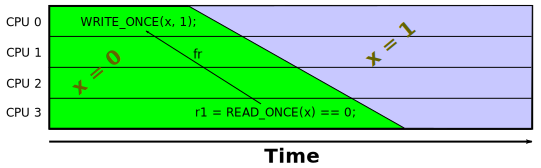
\includegraphics{memorder/fr}}
\caption{Load-to-Store is Counter-Temporal}
\label{fig:memorder:Load-to-Store is Counter-Temporal}
\end{figure}

This situation might seem completely counter-intuitive, but keep
in mind that the speed of light is finite and computers are of
non-zero size.
It therefore takes time for the effect of the \co{P2()}'s store to
\co{x} to propagate to \co{P1()}, which in turn means that it is possible
that \co{P1()}'s read from \co{x} happens much later in time, but
nevertheless still sees the old value of zero.
This situation is depicted in
\cref{fig:memorder:Load-to-Store is Counter-Temporal}:
Just because a load sees the old value does \emph{not} mean that
this load executed at an earlier time than did the store of the
new value.

Note that
\cref{lst:memorder:W+RWC Litmus Test With Release (No Ordering)}
also shows the limitations of memory-barrier pairing, given that
there are not two but three processes.
These more complex litmus tests can instead be said to have \emph{cycles},
where memory-barrier pairing is the special case of a two-thread cycle.
\begin{fcvref}[ln:formal:C-W+RWC+o-r+a-o+o-mb-o:whole]
The cycle in
\cref{lst:memorder:W+RWC Litmus Test With Release (No Ordering)}
goes through \co{P0()} (\clnref{P0:st,P0:sr}), \co{P1()} (\clnref{P1:la,P1:ld}),
\co{P2()} (\clnref{P2:st,P2:mb,P2:ld}), and back to \co{P0()} (\clnref{P0:st}).
The \co{exists} clause delineates this cycle:
The \co{1:r1=1} indicates that the \co{smp_load_acquire()} on \clnref{P1:la}
returned the value stored by the \co{smp_store_release()} on \clnref{P0:sr},
the \co{1:r2=0} indicates that the \co{WRITE_ONCE()} on \clnref{P2:st} came
too late to affect the value returned by the \co{READ_ONCE()} on \clnref{P1:ld},
and finally the \co{2:r3=0} indicates that the
\co{WRITE_ONCE()} on \clnref{P0:st} came too late to affect the value returned
by the \co{READ_ONCE()} on \clnref{P2:ld}.
In this case, the fact that the \co{exists} clause can trigger means that
the cycle is said to be \emph{allowed}.
In contrast, in cases where the \co{exists} clause cannot trigger,
the cycle is said to be \emph{prohibited}.
\end{fcvref}

\begin{listing}
\input{CodeSamples/formal/litmus/C-W+RWC+o-mb-o+a-o+o-mb-o@whole.fcv}
\caption{W+WRC Litmus Test With More Barriers}
\label{lst:memorder:W+WRC Litmus Test With More Barriers}
\end{listing}

\begin{fcvref}[ln:formal:C-W+RWC+o-r+a-o+o-mb-o:whole]
But what if we need to prohibit the cycle corresponding to the \co{exists}
clause on \clnref{exists} of
\cref{lst:memorder:W+RWC Litmus Test With Release (No Ordering)}?
One solution is to replace \co{P0()}'s \co{smp_store_release()}
with an \co{smp_mb()}, which
\cref{tab:memorder:Linux-Kernel Memory-Ordering Cheat Sheet}
shows to have not only cumulativity, but also propagation.
\end{fcvref}
The result is shown in
\cref{lst:memorder:W+WRC Litmus Test With More Barriers}
(\path{C-W+RWC+o-mb-o+a-o+o-mb-o.litmus}).

\QuickQuiz{
	\begin{fcvref}[ln:formal:C-W+RWC+o-r+a-o+o-mb-o:whole]
	But given that \co{smp_mb()} has the propagation property,
	why doesn't the \co{smp_mb()} on \clnref{P2:mb} of
	\cref{lst:memorder:W+RWC Litmus Test With Release (No Ordering)}
	prevent the \co{exists} clause from triggering?
	\end{fcvref}
}\QuickQuizAnswer{
	\begin{fcvref}[ln:formal:C-W+RWC+o-r+a-o+o-mb-o:whole]
	As a rough rule of thumb, the \co{smp_mb()} barrier's
	propagation property is sufficient to maintain ordering
	through only one load-to-store link between
	processes.
	Unfortunately,
	\cref{lst:memorder:W+RWC Litmus Test With Release (No Ordering)}
	has not one but two load-to-store links, with the
	first being from the \co{READ_ONCE()} on \clnref{P1:ld} to the
	\co{WRITE_ONCE()} on \clnref{P2:st} and the second being from
	the \co{READ_ONCE()} on \clnref{P2:ld} to the \co{WRITE_ONCE()}
	on \clnref{P0:st}.
	Therefore, preventing the \co{exists} clause from triggering
	should be expected to require not one but two
	instances of \co{smp_mb()}.
	\end{fcvref}

	As a special exception to this rule of thumb, a release-acquire
	chain can have one load-to-store link between processes
	and still prohibit the cycle.
}\QuickQuizEnd

\begin{figure}
\centering
\resizebox{\twocolumnwidth}{!}{\includegraphics{memorder/co}}
\caption{Store-to-Store is Counter-Temporal}
\label{fig:memorder:Store-to-Store is Counter-Temporal}
\end{figure}

For completeness,
\cref{fig:memorder:Store-to-Store is Counter-Temporal}
shows that the ``winning'' store among a group of stores to the
same variable is not necessarily the store that started last.
This should not come as a surprise to anyone who carefully examined
\cref{fig:memorder:A Variable With More Simultaneous Values}
on
\cpageref{fig:memorder:A Variable With More Simultaneous Values}.
One way to rationalize the counter-temporal properties of both
load-to-store and store-to-store ordering is to clearly distinguish
between the temporal order in which the store instructions executed on
the one hand, and the order in which the corresponding cacheline visited
the CPUs that executed those instructions on the other.
It is the cacheline-visitation order that defines the externally
visible ordering of the actual stores.
This cacheline-visitation order is not directly visible to the code
executing the store instructions, which results in the counter-intuitive
counter-temporal nature of load-to-store and store-to-store ordering.\footnote{
	In some hardware-multithreaded systems, the store would become
	visible to other CPUs in that same core as soon as the store
	reached the shared store buffer.
	As a result, such systems are non-multicopy atomic.}

\begin{listing}
\input{CodeSamples/formal/litmus/C-2+2W+o-wmb-o+o-wmb-o@whole.fcv}
\caption{2+2W Litmus Test With Write Barriers}
\label{lst:memorder:2+2W Litmus Test With Write Barriers}
\end{listing}

\QuickQuiz{
	But for litmus tests having only ordered stores, as shown in
	\cref{lst:memorder:2+2W Litmus Test With Write Barriers}
	(\path{C-2+2W+o-wmb-o+o-wmb-o.litmus}),
	research shows that the cycle is prohibited, even in weakly
	ordered systems such as \ARM\ and Power~\cite{test6-pdf}.
	Given that, is store-to-store ordering really \emph{always}
	counter-temporal???
}\QuickQuizAnswer{
	This litmus test is indeed a very interesting curiosity.
	Its ordering apparently occurs naturally given typical
	weakly ordered hardware design, which would normally be
	considered a great gift from the relevant laws of physics
	and cache-coherency-protocol mathematics.

	\begin{fcvref}[ln:formal:C-2+2W+o-wmb-o+o-wmb-o:whole]
	Unfortunately, no one has been able to come up with a software use
	case for this gift that does not have a much better alternative
	implementation.
	Therefore, neither the C11 nor the Linux kernel memory models
	provide any guarantee corresponding to
	\cref{lst:memorder:2+2W Litmus Test With Write Barriers}.
	This means that the \co{exists} clause on \clnref{exists} can
	trigger.
	\end{fcvref}

\begin{listing}
\input{CodeSamples/formal/litmus/C-2+2W+o-o+o-o@whole.fcv}
\caption{2+2W Litmus Test (No Ordering)}
\label{lst:memorder:2+2W Litmus Test (No Ordering)}
\end{listing}

	Of course, without the barrier, there are no ordering
	guarantees, even on real weakly ordered hardware, as shown in
	\cref{lst:memorder:2+2W Litmus Test (No Ordering)}
	(\path{C-2+2W+o-o+o-o.litmus}).
}\QuickQuizEnd

But sometimes time really is on our side.
Read on!

\subsubsection{Happens-Before}
\label{sec:memorder:Happens-Before}

As shown in
\cref{fig:memorder:Store-to-Load is Temporal},
on platforms without user-visible speculation, if a load returns the value
from a particular store, then, courtesy of the finite speed of light and
the non-zero size of modern computing systems, the store absolutely has
to have executed at an earlier time than did the load.
This means that carefully constructed programs can rely on the
passage of time itself as a memory-ordering operation.

\QuickQuiz{
	Why don't we just stick to sanely ordered CPU families like x86,
	so that time will \emph{always} be on our side???
}\QuickQuizAnswer{
	Sorry to be the one to break it to you, but x86 CPUs have
	store buffers and they are not afraid to use them.

	The data shown in
	\crefrange{fig:memorder:x86 CPUs Can Disagree}{fig:memorder:Store-to-Load is Temporal on x86}
	was obtained from a two-socket x86 system having a total of 80
	hardware threads.\footnote{
		\co{Intel(R) Xeon(R) Gold 6138 CPU @ 2.00GHz},
		for those wanting more details.}

\begin{figure}
\centering
\resizebox{\twocolumnwidth}{!}{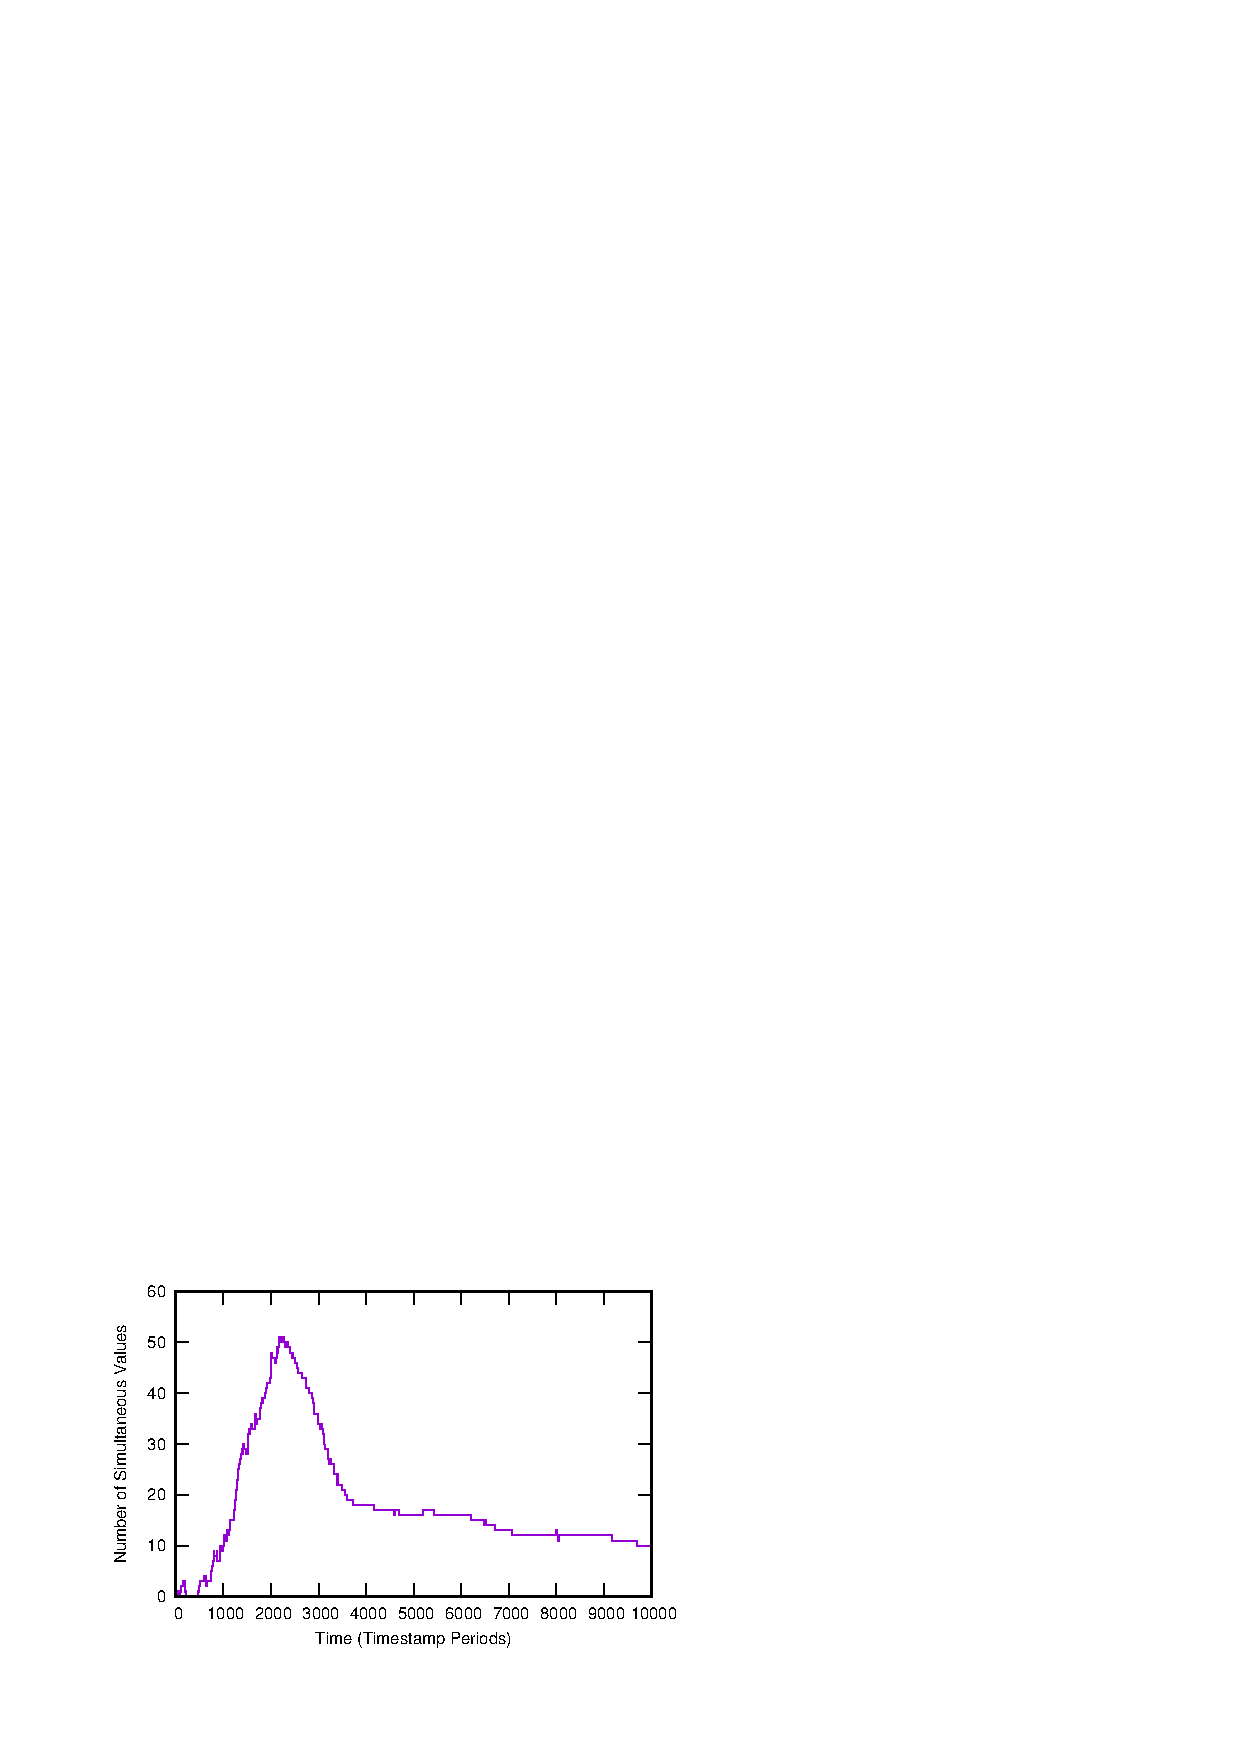
\includegraphics{CodeSamples/cpu/data/coe-nvals}}
\caption{x86 CPUs Can Disagree}
\label{fig:memorder:x86 CPUs Can Disagree}
\end{figure}

	\Cref{fig:memorder:x86 CPUs Can Disagree} is from a program
	similar to the one that generated
	\cref{fig:memorder:A Variable With More Simultaneous Values}
	on
	\cpageref{fig:memorder:A Variable With More Simultaneous Values},
	but showing the number of distinct opinions per unit time, where
	each timestamp period is 0.5~nanoseconds.\footnote{
		Recall that each CPU writes its own number to a single
		shared variable, which each CPU repeatedly polls,
		recording time and value at each change in value.}
	As you can see, there is a significant period of time during
	which there are more than 40 distinct opinions as to the value
	of a single shared variable.
	Even on x86.

\begin{figure}
\centering
\resizebox{.85\twocolumnwidth}{!}{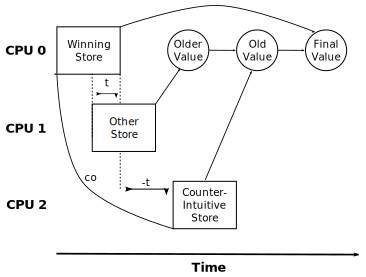
\includegraphics{memorder/co-hopes}}
\caption{Is Store-to-Store Counter-Temporal on x86?}
\label{fig:memorder:Is Store-to-Store Counter-Temporal on x86?}
\end{figure}

	But perhaps we might hope that on x86, the last CPU to execute its
	store in global time order would ``win'', that is, the final value
	of the shared variable would be that of that last store.
	If so, any store starting after the ``winning'' store finished would
	overwrite the winning store.
	In contrast, we know that on weakly ordered systems, a
	counter-intuitive store such as that shown at the bottom of
	\cref{fig:memorder:Is Store-to-Store Counter-Temporal on x86?}
	could read the old value, despite the fact that it started
	$t$ timestamp periods after the winning store completed,
	as depicted in the figure by the time interval that is labelled
	$-t$.\footnote{
		That is completed from the viewpoint of the instruction
		stream containing that store.
		The value stored might well remain in the store buffer
		for long afterwards.}

\begin{figure}
\centering
\resizebox{\twocolumnwidth}{!}{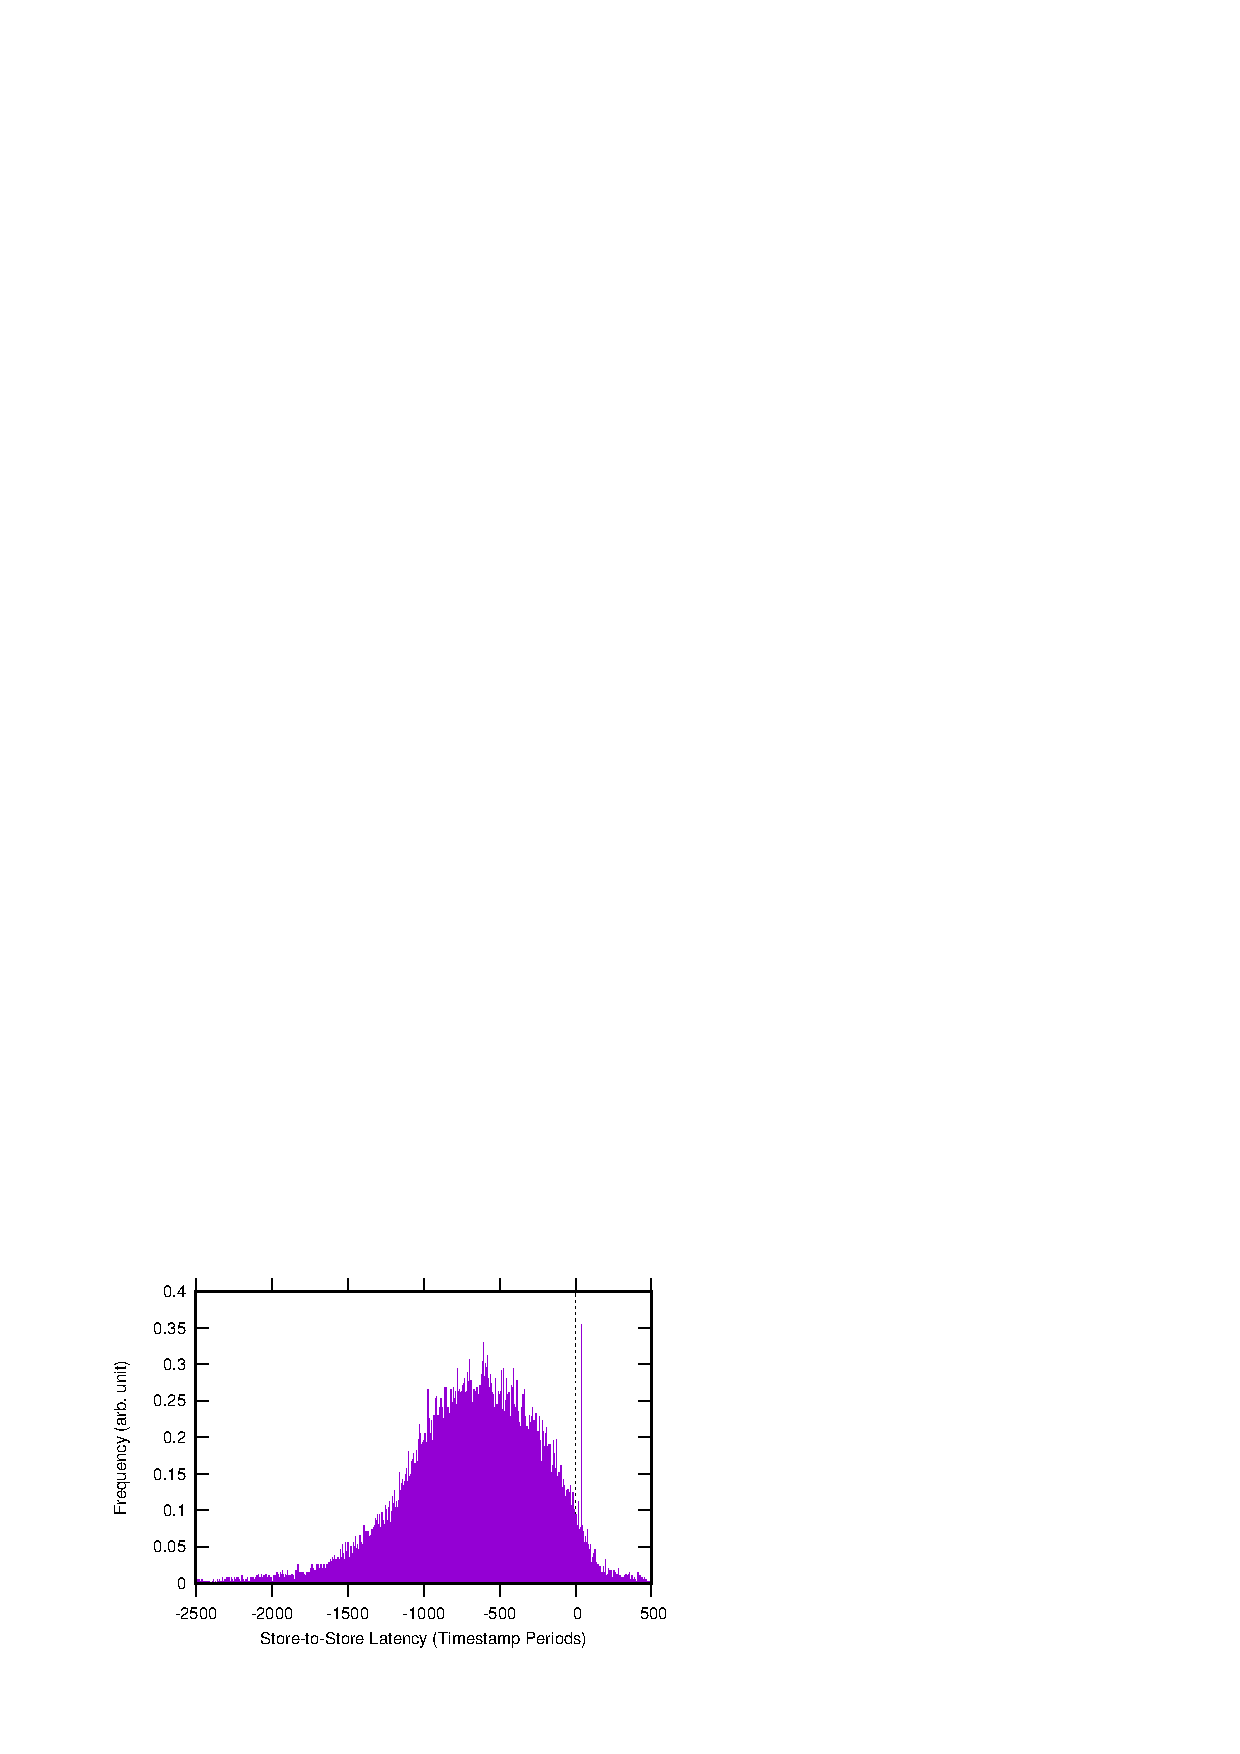
\includegraphics{CodeSamples/cpu/data/coe}}
\caption{Store-to-Store is Counter-Temporal on x86}
\label{fig:memorder:Store-to-Store is Counter-Temporal on x86}
\end{figure}

	However,
	\cref{fig:memorder:Store-to-Store is Counter-Temporal on x86}
	dashes any fond hope of x86 refusing to indulge in
	counter-intuitive stores.
	The data in this figure summarizes the results from 79,000 runs
	of the type that generated
	\cref{fig:memorder:x86 CPUs Can Disagree},
	and is a histogram of the minimum time elapsed between the start of
	a non-winning CPU's store and the end of the winning CPU's store.
	Of course, if this value is negative, the winning store completed
	(though its value might not have propagated past the store buffer)
	before some other store even started.
	And the negative-time data points in that figure show that
	this counter-temporal behavior really happens most of the time,
	even on x86.

\begin{figure}
\centering
\resizebox{.6\twocolumnwidth}{!}{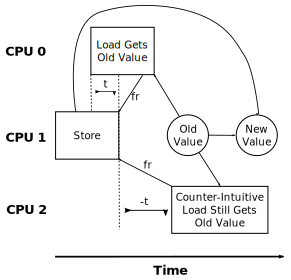
\includegraphics{memorder/fr-hopes}}
\caption{Is Load-to-Store Counter-Temporal on x86?}
\label{fig:memorder:Is Load-to-Store Counter-Temporal on x86?}
\end{figure}

	But perhaps we could instead hope that once a store had
	executed, any future load from that same variable might
	be guaranteed to return the new value.
	In contrast, we know that on weakly ordered systems, a
	counter-intuitive load such as that shown at the bottom
	of
	\cref{fig:memorder:Is Load-to-Store Counter-Temporal on x86?}
	could return the old value, despite having started $t$
	timestamp periods after the end of the store, again, as
	depicted in the figure by the $-t$.

\begin{figure}
\centering
\resizebox{\twocolumnwidth}{!}{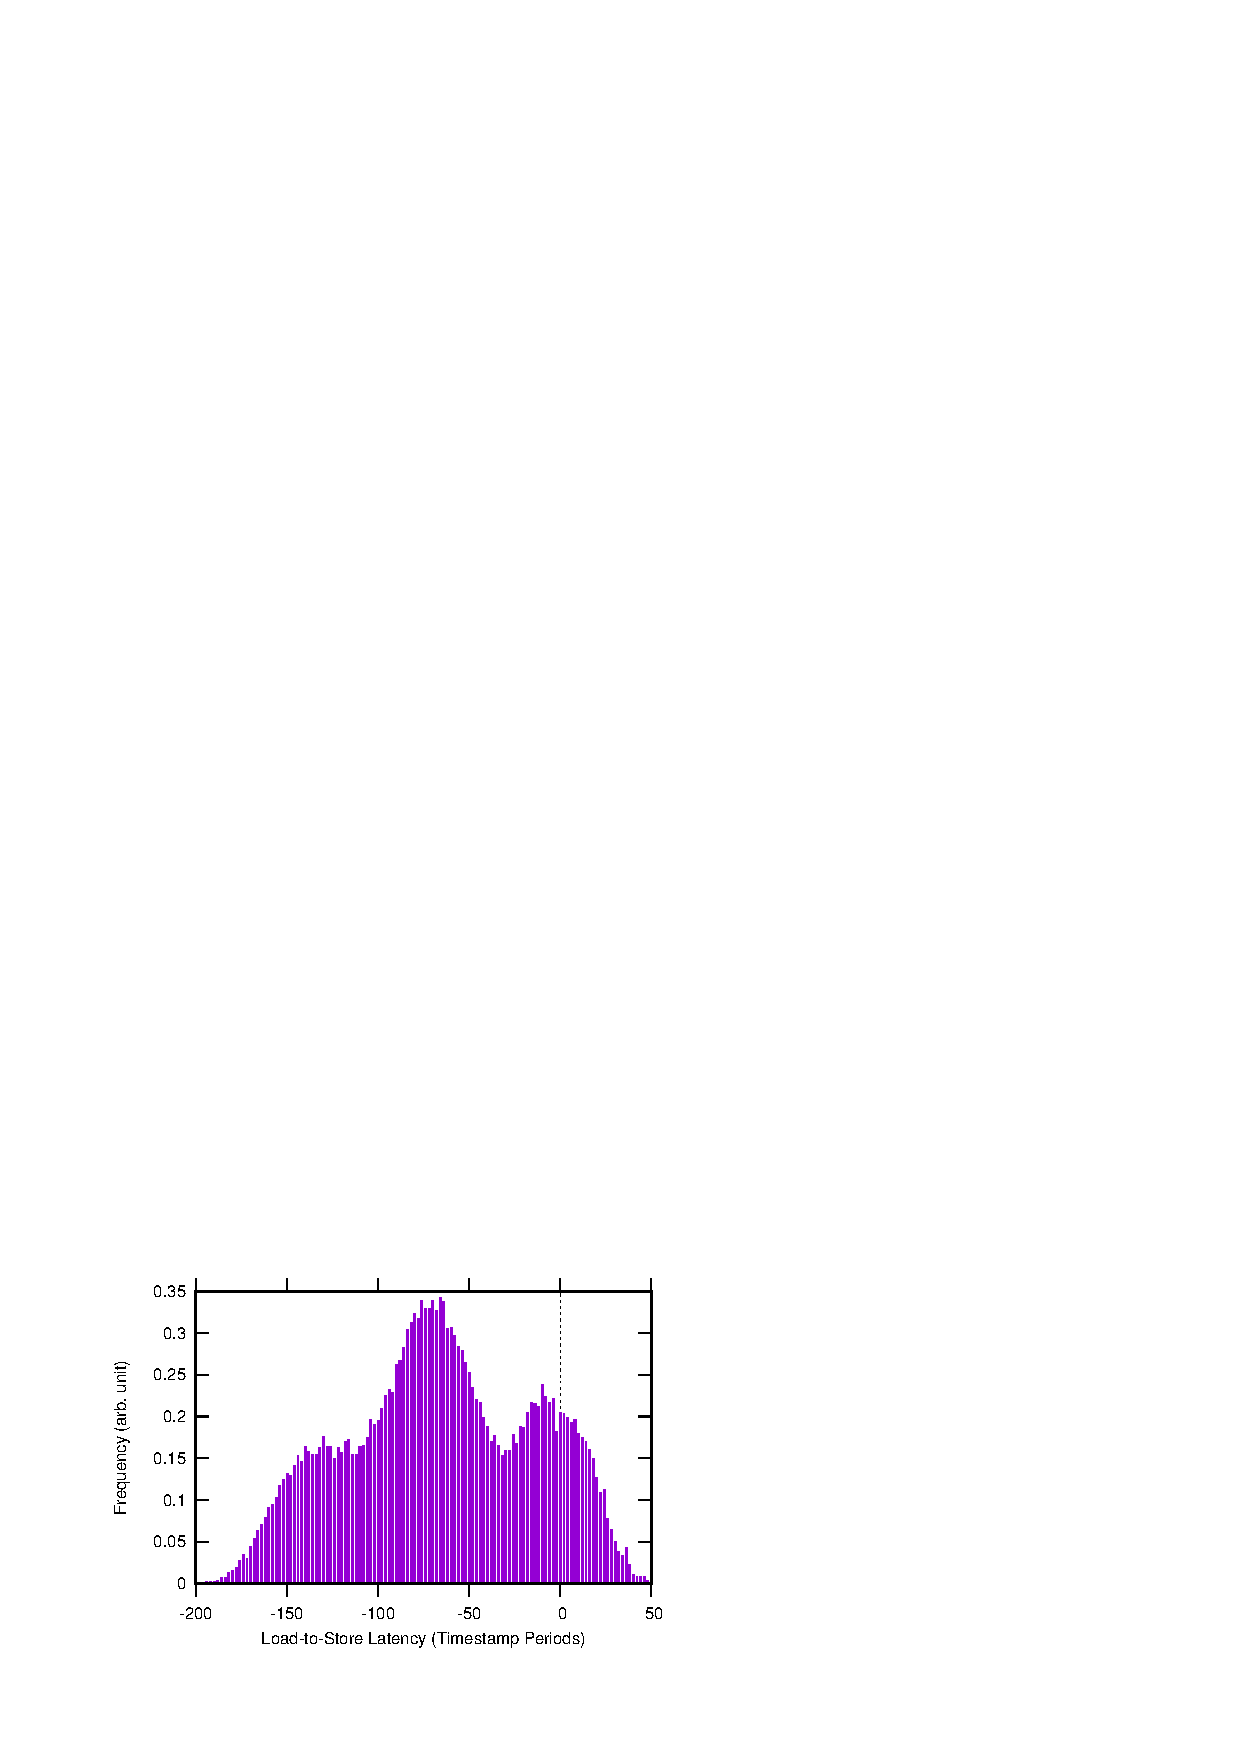
\includegraphics{CodeSamples/cpu/data/fre}}
\caption{Load-to-Store is Counter-Temporal on x86}
\label{fig:memorder:Load-to-Store is Counter-Temporal on x86}
\end{figure}

	However,
	\cref{fig:memorder:Load-to-Store is Counter-Temporal on x86}
	dashes any fond hopes that loads executing after a given store
	would see that store's value (or some later value).
	This data is generated by 1,000 runs of a program in which the
	parent thread spawns the children, each of which polls a shared
	variable.
	After all the children are running, the parent writes a new
	value to the shared variable.
	The quantity histogrammed in the figure is the time from just
	after the store until just before the last load of the old value.
	And most of these data points lie on the negative x~axis, clearly
	demonstrating the counter-temporal nature of cross-thread
	load-to-store.

\begin{figure}
\centering
\resizebox{\twocolumnwidth}{!}{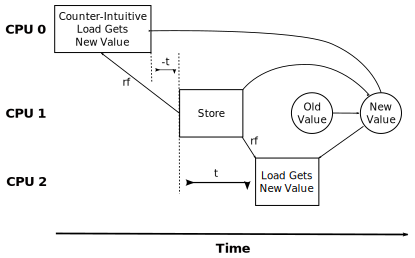
\includegraphics{memorder/rf-hopes}}
\caption{Is Store-to-Load Counter-Temporal on x86?}
\label{fig:memorder:Is Store-to-Load Counter-Temporal on x86?}
\end{figure}

\begin{figure}
\centering
\resizebox{\twocolumnwidth}{!}{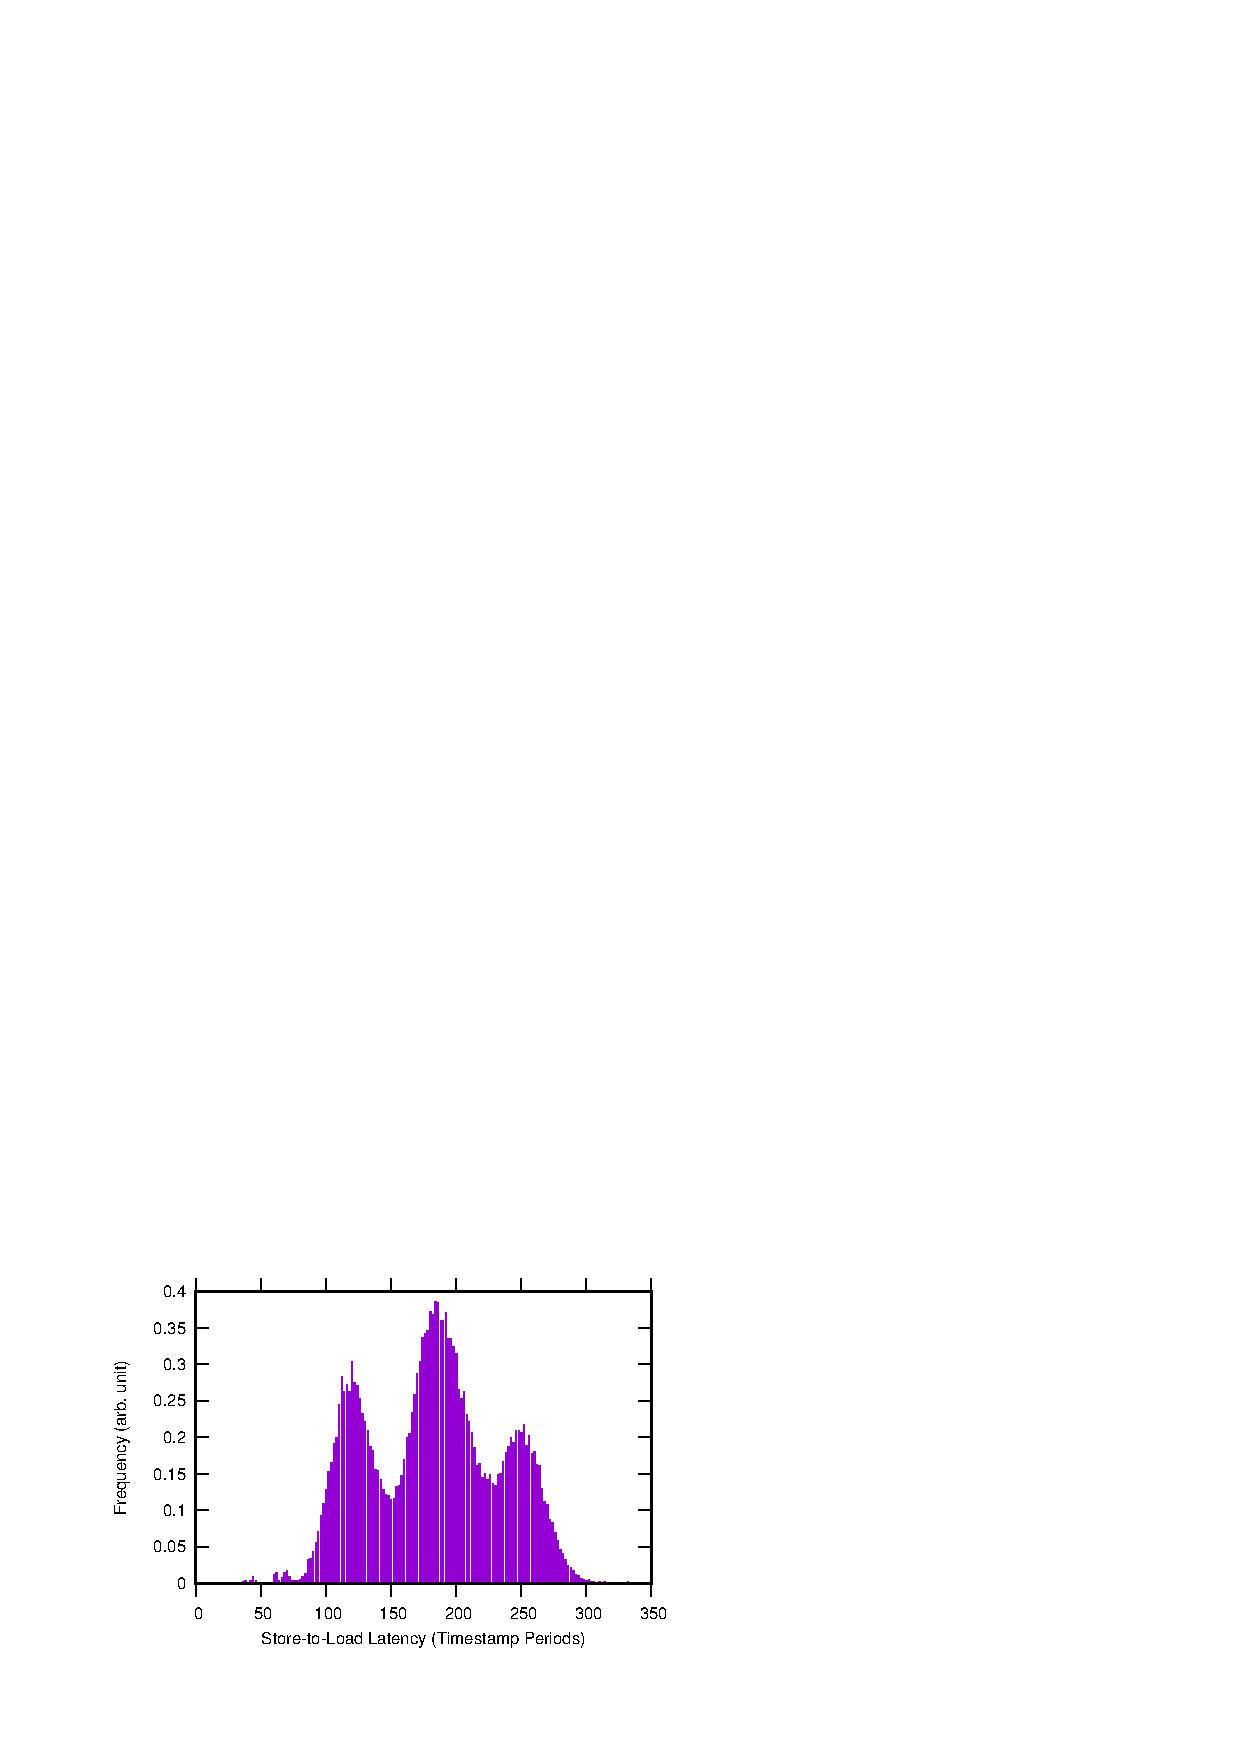
\includegraphics{CodeSamples/cpu/data/rfe}}
\caption{Store-to-Load is Temporal on x86}
\label{fig:memorder:Store-to-Load is Temporal on x86}
\end{figure}

	It is only reasonable to assume that a load that ends before
	a store starts will be unable to load that store's value,
	as shown in
	\cref{fig:memorder:Is Store-to-Load Counter-Temporal on x86?},
	even on weakly ordered systems.
	And the data points from all 1,000 runs shown in
	\cref{fig:memorder:Store-to-Load is Temporal on x86},
	lie on the positive x~axis,
	so in this case, our temporal hopes have been fulfilled.

	These results should be no surprise.
	Even on x86, the cache line shuttles between cores and sockets, and
	\cref{fig:memorder:x86 CPUs Can Disagree}
	indicates that a given store can remain in its CPU's store buffer
	for a a number of microseconds, which is more than enough time
	for today's multi-GHz CPUs to detect counter-temporal behavior.

	However, for the store-to-load case, the laws of physics guarantee
	temporal ordering because the finite speed of light and the non-zero
	size of atoms guarantees that some time will pass between a store
	and a load on some other CPU that reads that store's value.

	Alert readers may have noticed that the distribution shown in
	\cref{fig:memorder:Store-to-Store is Counter-Temporal on x86}
	is nearly monomodal, which those in
	\cref{fig:memorder:Load-to-Store is Counter-Temporal on x86}
	and
	\cref{fig:memorder:Store-to-Load is Temporal on x86}
	are decidedly trimodal.
	Such readers are encouraged to consider why that might be,
	perhaps referring to \path{CodeSamples/cpu/perftemporal.sh} and
	the scripts and programs that it invokes.

	And all readers are encouraged to note that even on relatively
	strongly ordered CPUs such as x86, store-to-store and
	load-to-store IPC links can be counter-temporal.
}\QuickQuizEnd

\begin{figure}
\centering
\resizebox{\twocolumnwidth}{!}{\includegraphics{memorder/rf}}
\caption{Store-to-Load is Temporal}
\label{fig:memorder:Store-to-Load is Temporal}
\end{figure}

\begin{listing}
\input{CodeSamples/formal/litmus/C-LB+a-o+o-data-o+o-data-o@whole.fcv}
\caption{LB Litmus Test With One Acquire}
\label{lst:memorder:LB Litmus Test With One Acquire}
\end{listing}

Of course, just the passage of time by itself is not enough, as
was seen in
\cref{lst:memorder:Load-Buffering Litmus Test (No Ordering)}
on
\cpageref{lst:memorder:Load-Buffering Litmus Test (No Ordering)},
which has nothing but store-to-load links and, because it provides
absolutely no ordering, still can trigger its \co{exists} clause.
However, as long as each thread provides even the weakest possible
ordering, \co{exists} clause would not be able to trigger.
For example,
\cref{lst:memorder:LB Litmus Test With One Acquire}
(\path{C-LB+a-o+o-data-o+o-data-o.litmus})
shows \co{P0()} ordered with an \co{smp_load_acquire()} and
both \co{P1()} and \co{P2()} ordered with data dependencies.
These orderings, which are close to the top of
\cref{tab:memorder:Linux-Kernel Memory-Ordering Cheat Sheet},
suffice to prevent the \co{exists} clause from triggering.

\QuickQuiz{
	Can you construct a litmus test like that in
	\cref{lst:memorder:LB Litmus Test With One Acquire}
	that uses \emph{only} dependencies?
}\QuickQuizAnswer{
	\Cref{lst:memorder:LB Litmus Test With No Acquires}
	shows a somewhat nonsensical but very real example.
	Creating a more useful (but still real) litmus test is left
	as an exercise for the reader.

\begin{listing}
\input{CodeSamples/formal/litmus/C-LB+o-data-o+o-data-o+o-data-o@whole.fcv}
\caption{LB Litmus Test With No Acquires}
\label{lst:memorder:LB Litmus Test With No Acquires}
\end{listing}
}\QuickQuizEnd

An important use of time for ordering memory accesses is covered in the
next section.

\subsubsection{Release-Acquire Chains}
\label{sec:memorder:Release-Acquire Chains}

A minimal release-acquire chain was shown in
\cref{lst:memorder:Enforcing Ordering of Load-Buffering Litmus Test}
on
\cpageref{lst:memorder:Enforcing Ordering of Load-Buffering Litmus Test},
but these chains can be much longer, as shown in
\cref{lst:memorder:Long LB Release-Acquire Chain}
(\path{C-LB+a-r+a-r+a-r+a-r.litmus}).
The longer the release-acquire chain, the more ordering is gained
from the passage of time, so that no matter how many threads are
involved, the corresponding \co{exists} clause cannot trigger.

\begin{listing}
\input{CodeSamples/formal/litmus/C-LB+a-r+a-r+a-r+a-r@whole.fcv}
\caption{Long LB Release-Acquire Chain}
\label{lst:memorder:Long LB Release-Acquire Chain}
\end{listing}

Although release-acquire chains are inherently store-to-load creatures,
it turns out that they can tolerate one load-to-store step, despite
such steps being counter-temporal, as shown in
\cref{fig:memorder:Load-to-Store is Counter-Temporal}
on
\cpageref{fig:memorder:Load-to-Store is Counter-Temporal}.
For example,
\cref{lst:memorder:Long ISA2 Release-Acquire Chain}
(\path{C-ISA2+o-r+a-r+a-r+a-o.litmus})
shows a three-step release-acquire chain, but where \co{P3()}'s
final access is a \co{READ_ONCE()} from \co{x0}, which is
accessed via \co{WRITE_ONCE()} by \co{P0()}, forming a non-temporal
load-to-store link between these two processes.
\begin{fcvref}[ln:formal:litmus:C-ISA2+o-r+a-r+a-r+a-o:whole]
However, because \co{P0()}'s \co{smp_store_release()} (\clnref{P0:rel})
is cumulative, if \co{P3()}'s \co{READ_ONCE()} returns zero,
this cumulativity will force the \co{READ_ONCE()} to be ordered
before \co{P0()}'s \co{smp_store_release()}.
In addition, the release-acquire chain
(\clnref{P0:rel,P1:acq,P1:rel,P2:acq,P2:rel,P3:acq})
forces \co{P3()}'s \co{READ_ONCE()} to be ordered after \co{P0()}'s
\co{smp_store_release()}.
Because \co{P3()}'s \co{READ_ONCE()} cannot be both before and after
\co{P0()}'s \co{smp_store_release()}, either or both of two things must
be true:
\end{fcvref}

\begin{listing}
\input{CodeSamples/formal/litmus/C-ISA2+o-r+a-r+a-r+a-o@whole.fcv}
\caption{Long ISA2 Release-Acquire Chain}
\label{lst:memorder:Long ISA2 Release-Acquire Chain}
\end{listing}

\begin{enumerate}
\item	\co{P3()}'s \co{READ_ONCE()} came after \co{P0()}'s
	\co{WRITE_ONCE()}, so that the \co{READ_ONCE()} returned
	the value two, so that the \co{exists} clause's \co{3:r2=0}
	is false.
\item	The release-acquire chain did not form, that is, one or more
	of the \co{exists} clause's \co{1:r2=2}, \co{2:r2=2}, or \co{3:r1=2}
	is false.
\end{enumerate}

Either way, the \co{exists} clause cannot trigger, despite this litmus
test containing a notorious load-to-store link between
\co{P3()} and \co{P0()}.
But never forget that release-acquire chains can tolerate only one
load-to-store link, as was seen in
\cref{lst:memorder:W+RWC Litmus Test With Release (No Ordering)}.

\begin{listing}
\input{CodeSamples/formal/litmus/C-Z6.2+o-r+a-r+a-r+a-o@whole.fcv}
\caption{Long Z6.2 Release-Acquire Chain}
\label{lst:memorder:Long Z6.2 Release-Acquire Chain}
\end{listing}

Release-acquire chains can also tolerate a single store-to-store step,
as shown in
\cref{lst:memorder:Long Z6.2 Release-Acquire Chain}
(\path{C-Z6.2+o-r+a-r+a-r+a-o.litmus}).
\begin{fcvref}[ln:formal:C-Z6.2+o-r+a-r+a-r+a-o:whole]
As with the previous example, \co{smp_store_release()}'s cumulativity
combined with the temporal nature of the release-acquire chain
prevents the \co{exists} clause on \clnref{exists} from triggering.
\end{fcvref}

\begin{listing}
\input{CodeSamples/formal/litmus/C-Z6.2+o-r+a-o+o-mb-o@whole.fcv}
\caption{Z6.2 Release-Acquire Chain (Ordering?)}
\label{lst:memorder:Z6.2 Release-Acquire Chain (Ordering?)}
\end{listing}

\QuickQuiz{
	Suppose we have a short release-acquire chain along with one
	load-to-store link and one store-to-store link, like that shown in
	\cref{lst:memorder:Z6.2 Release-Acquire Chain (Ordering?)}.
	Given that there is only one of each type of non-store-to-load
	link, the \co{exists} cannot trigger, right?
}\QuickQuizAnswer{
	Wrong.
	It is the number of non-store-to-load links that matters.
	If there is only one non-store-to-load link, a release-acquire
	chain can prevent the \co{exists} clause from triggering.
	However, if there is more than one non-store-to-load link,
	be they store-to-store, load-to-store, or any combination
	thereof, it is necessary to have at least one full barrier
	(\co{smp_mb()} or better) between each non-store-to-load link.
	In
	\cref{lst:memorder:Z6.2 Release-Acquire Chain (Ordering?)},
	preventing the \co{exists} clause from triggering therefore requires
	an additional full barrier between either \co{P0()}'s or
	\co{P1()}'s accesses.
}\QuickQuizEnd

\begin{listing}
\input{CodeSamples/formal/litmus/C-MP+o-r+a-o@whole.fcv}
\caption{A Release-Acquire Chain Ordering Multiple Accesses}
\label{lst:memorder:A Release-Acquire Chain Ordering Multiple Accesses}
\end{listing}

\begin{listing}
\input{CodeSamples/formal/litmus/C-MPO+o-r+a-o+o@whole.fcv}
\caption{A Release-Acquire Chain With Added Store (Ordering?)}
\label{lst:memorder:A Release-Acquire Chain With Added Store (Ordering?)}
\end{listing}

But beware:
Adding a second store-to-store link allows the correspondingly updated
\co{exists} clause to trigger.
To see this, review
\cref{lst:memorder:A Release-Acquire Chain Ordering Multiple Accesses,%
lst:memorder:A Release-Acquire Chain With Added Store (Ordering?)},
which have identical \co{P0()} and \co{P1()} processes.
The only code difference is that
\cref{lst:memorder:A Release-Acquire Chain With Added Store (Ordering?)}
has an additional \co{P2()} that does an \co{smp_store_release()} to
the \co{x2} variable that \co{P0()} releases and \co{P1()} acquires.
The \co{exists} clause is also adjusted to exclude executions in which
\co{P2()}'s \co{smp_store_release()} precedes that of \co{P0()}.

Running the litmus test in
\cref{lst:memorder:A Release-Acquire Chain With Added Store (Ordering?)}
shows that the addition of \co{P2()} can totally destroy the
ordering from the release-acquire chain.
Therefore, when constructing release-acquire chains, please take care
to construct them properly.

\QuickQuiz{
	There are store-to-load links, load-to-store links, and
	store-to-store links.
	But what about load-to-load links?
}\QuickQuizAnswer{
	The problem with the concept of load-to-load links is that
	if the two loads from the same variable return the same
	value, there is no way to determine their ordering.
	The only way to determine their ordering is if they return
	different values, in which case there had to have been an
	intervening store.
	And that intervening store means that there is no load-to-load
	link, but rather a load-to-store link followed by a
	store-to-load link.
}\QuickQuizEnd

In short, properly constructed release-acquire chains form a peaceful
island of intuitive bliss surrounded by a strongly counter-intuitive
sea of more complex memory-ordering constraints.

\subsection{A Counter-Intuitive Case Study}
\label{sec:memorder:A Counter-Intuitive Case Study}

This section will revisit
\cref{lst:memorder:R Litmus Test With Write Memory Barrier (No Ordering)}
on \cpageref{lst:memorder:R Litmus Test With Write Memory Barrier (No Ordering)},
which was presented in the answer to
\QuickQuizARef{\MemorderQQLitmusTestR}.
This litmus test has only two threads, with the stores in \co{P0()}
being ordered by \co{smp_wmb()} and the accesses in \co{P1()} being
ordered by \co{smp_mb()}.
Despite this litmus test's small size and heavy ordering, the
counter-intuitive outcome shown in the \co{exists} clause is in fact
allowed.

One way to look at this was presented in the answer to
\QuickQuizARef{\MemorderQQLitmusTestR}, namely that the link from
\co{P0()} to \co{P1()} is a store-to-store link, and that back
from \co{P1()} to \co{P0()} is a store-to-store link.
Both links are counter-temporal, thus requiring full memory barriers
in both processes.
Revisiting
\cref{fig:memorder:Store-to-Store is Counter-Temporal,%
fig:memorder:Store-to-Load is Temporal}
shows that these counter-temporal links give the hardware considerable
latitude.

But that raises the question of exactly how hardware would go about using
this latitude to satisfy the \co{exists} clause in
\cref{lst:memorder:R Litmus Test With Write Memory Barrier (No Ordering)}.
There is no known ``toy'' hardware implementation that can do this, so
let us instead study the sequence of steps that the PowerPC architecture
goes through to make this happen.

The first step in this study is to translate
\cref{lst:memorder:R Litmus Test With Write Memory Barrier (No Ordering)}
to a PowerPC assembly language litmus test
(\cref{sec:formal:Anatomy of a Litmus Test} on
\cpageref{sec:formal:Anatomy of a Litmus Test}):

\begin{fcvlabel}[ln:memorder:inline:ppcasmr]
\begin{VerbatimN}[samepage=true,commandchars=\@\[\]]
PPC R+lwsync+sync
{
0:r1=1; 0:r2=x; 0:r4=y;		@lnlbl[init0]
1:r1=2; 1:r2=y; 1:r4=x;		@lnlbl[init1]
}
 P0           | P1           ;	@lnlbl[procs]
 stw r1,0(r2) | stw r1,0(r2) ;	@lnlbl[stores]
 lwsync       | sync         ;	@lnlbl[barriers]
 stw r1,0(r4) | lwz r3,0(r4) ;	@lnlbl[storeload]
exists (y=2 /\ 1:r3=0)		@lnlbl[exists]
\end{VerbatimN}
\end{fcvlabel}

\begin{fcvref}[ln:memorder:inline:ppcasmr]
The first line identifies the type of test (\co{PPC}) and gives
the test's name.
\Clnref{init0,init1} initialize \co{P0()}'s and \co{P1()}'s registers,
respectively.
\Clnrefrange{procs}{storeload} show the PowerPC assembly
statements corresponding to the C code from
\cref{lst:memorder:R Litmus Test With Write Memory Barrier (No Ordering)},
with the first column being the code for \co{P0()} and the second column
being the code for \co{P1()}.
\Clnref{stores} shows the initial \co{WRITE_ONCE()} calls in both columns;
the columns of \clnref{barriers} show the \co{smp_wmb()} and \co{smp_mb()}
for \co{P0()} and \co{P1()}, respectively;
the columns of \clnref{storeload} shows \co{P0()}'s \co{WRITE_ONCE()} and
\co{P1()}'s \co{READ_ONCE()}, respectively;
and finally \clnref{exists} shows the \co{exists} clause.
\end{fcvref}

In order for this \co{exists} clause to be satisfied, \co{P0()}'s
\co{stw} to \co{y} must precede that of \co{P1()}, but \co{P1()}'s
later \co{lwz} from \co{x} must precede \co{P0()}'s \co{stw} to \co{x}.
Seeing how this can happen requires a rough understanding of the
following PowerPC terminology.

\begin{description}[style=nextline]

\item[Instruction commit:]
This can be thought of as the execution of that instruction as opposed
to the memory-system consequences of having executed that instruction.

\item[Write reaching coherence point:]
This can be thought of as the value written being deposited into the
corresponding cache line.

\item[Partial coherence commit:]
This can be thought of as the system having worked out the order in which
a pair of values written will be deposited into the corresponding cache
line, but potentially well before that cache line arrives.
Some might argue that the data in
\cref{fig:memorder:A Variable With More Simultaneous Values}
suggests that real PowerPC hardware does in fact use partial coherence
commits to handle concurrent stores by multiple hardware threads within
a single core.

\item[Write propagate to thread:]
This occurs when a second hardware thread becomes aware of the first
hardware thread's write.
The time at which a write propagates to a given thread might not have
any relation to cache-line movement.
For example, if a pair of threads share a store buffer, they might see
each others' writes long before the cache line gets involved.
On the other hand, if a pair of hardware threads are widely separated,
the first thread's write's value might have been deposited into the
corresponding cache line long before the second thread learns of that
write.

\item[Barrier propagate to thread:]
Hardware threads make each other aware of memory-barrier instructions
as needed by propagating them to each other.

\item[Acknowledge \tco{sync}:]
The PowerPC \co{sync} instruction implements the Linux kernel's
\co{smp_mb()} full barrier.
And one reason that the \co{sync} instruction provides such strong
ordering is that each \co{sync} is not only propagated to other hardware
threads, but these other threads must also acknowledge each \co{sync}.
This two-way communication allows the hardware threads to cooperate
to produce the required strong global ordering.

\end{description}

\begin{figure*}[tbp]
\centering
\resizebox{\textwidth}{!}{\includegraphics{memorder/PPCMEM0.png}}
\caption{PPCMEM Initial R State}
\label{fig:memorder:PPCMEM Initial R State}
\end{figure*}

\begin{figure*}[tbp]
\centering
\resizebox{\textwidth}{!}{\includegraphics{memorder/PPCMEM1.png}}
\caption{PPCMEM First R Step}
\label{fig:memorder:PPCMEM First R Step}
\end{figure*}

We are now ready to step through the PowerPC sequence of events that
satisfies the above \co{exists} clause.

To best understand this, please follow along at
\url{https://www.cl.cam.ac.uk/~pes20/ppcmem/index.html},
carefully copying the above assembly-language litmus test into the pane.
The result should look as shown in
\cref{fig:memorder:PPCMEM Initial R State}, give or take space characters.
Click on the ``Interactive'' button in the lower left, which, after a
short delay, should produce a display as shown in
\cref{fig:memorder:PPCMEM First R Step}.
If the ``Interactive'' button refuses to do anything, this usually means
that there is a syntax error, for example, a spurious newline character
might have been introduced during the copy-paste operation.

This display has one clickable link in each section displaying thread
state, and as the ``Commit'' in each link suggests, these links commit
each thread's first \co{stw} instruction.
If you prefer, you can instead click on the corresponding links listed
under ``Enabled transitions'' near the bottom of the screen.
Note well that some of the later memory-system transitions will appear
in the upper ``Storage subsystem state'' section of this display.

The following sequence of clicks demonstrates how the \co{exists} clause
can be satisfied:

\begin{enumerate}
\item	Commit \co{P0()}'s first \co{stw} instruction (to \co{x}).
\item	Commit \co{P1()}'s \co{stw} instruction.
\item	Commit \co{P0()}'s \co{lwsync} instruction.
\item	Commit \co{P0()}'s second \co{stw} instruction (to \co{y}).
\item	Commit \co{P1()}'s \co{sync} instruction.
\item	At this point, there should be no clickable links in either of
	the two sections displaying thread state, but there should be
	quite a few of them up in the ``Storage subsystem state''.
	The following steps tell you which of them to click on.
\item	\co{Partial coherence commit: c:W y=1 -> d:W y=2}.
	This commits the system to processing \co{P0()}'s store to
	\co{y} before \co{P1()}'s store even though neither store
	has reached either the coherence point or any other thread.
	One might imagine partial coherence commits happening within a
	store buffer that is shared by multiple hardware threads
	that are writing to the same variable.
\item	\co{Write propagate to thread: d:W y=2 to Thread 0}.
	This is necessary to allow \co{P1()}'s \co{sync} instruction
	to propagate to \co{P0()}.
\item	\co{Barrier propagate to thread: e:Sync  to Thread 0}.
\item	\co{Write reaching coherence point: a:W x=1}.
\item	\co{Write reaching coherence point: c:W y=1}.
\item	\co{Write reaching coherence point: d:W y=2}.
	These three operations were required in order to allow \co{P0()}
	to acknowledge \co{P1()}'s \co{sync} instruction.
\item	\co{Acknowledge sync: Sync e:Sync}.
\item	Back down in thread \co{P1()}'s state, click on \co{Read i:W
	x=0}, which loads the value zero, thus satisfying the \co{exists}
	clause.
	All that remains is cleanup, which can be carried out in any order.
\item	Commit \co{P1()}'s \co{lwz} instruction.
\item	\co{Write propagate to thread: a:W x=1 to Thread 1}.
\item	\co{Barrier propagate to thread: b:Lwsync  to Thread 1}.
\end{enumerate}

\begin{figure*}[tbp]
\centering
\resizebox{\textwidth}{!}{\includegraphics{memorder/PPCMEMfinal.png}}
\caption{PPCMEM Final R State}
\label{fig:memorder:PPCMEM Final R State}
\end{figure*}

At this point, you should see something like
\cref{fig:memorder:PPCMEM Final R State}.
Note that the satisified \co{exists} clause is shown in blue near the
bottom, confirming that this counter-intuitive really can happen.
If you wish, you can click on ``Undo'' to explore other options or
click on ``Reset'' to start over.
It can be very helpful to carry out these steps in different orders
to better understand how a non-multicopy-atomic architecture operates.

\QuickQuiz{
	What happens if that \co{lwsync} instruction is instead a
	\co{sync} instruction?
}\QuickQuizAnswer{
	The counter-intuitive outcome cannot happen.
	(Try it!)
}\QuickQuizEnd

Although a full understanding of how this counter-intuitive outcome
happens would require hardware details that are beyond the scope of
this book, this exercise should provide some helpful intuitions.
Or perhaps more accurately, destroy some counter-productive intuitions.

% @@@ Exercises?
% @@@ Hardware details from Appendix?

\section{Compile-Time Consternation}
\label{sec:memorder:Compile-Time Consternation}
%
\epigraph{Science increases our power in proportion as it lowers our pride.}
	 {Claude Bernard}

Most languages, including C, were developed on uniprocessor systems
by people with little or no parallel-programming experience.
As a result, unless explicitly told otherwise, these languages assume
that the current CPU is the only thing that is reading or writing memory.
This in turn means that these languages' compilers' optimizers
are ready, willing, and oh so able to make dramatic changes to the
order, number, and sizes of memory references that your program
executes.
In fact, the reordering carried out by hardware can seem quite tame
by comparison.

This section will help you tame your compiler, thus avoiding a great
deal of compile-time consternation.
\Cref{sec:memorder:Memory-Reference Restrictions}
describes how to keep the compiler from destructively optimizing
your code's memory references,
\cref{sec:memorder:Address- and Data-Dependency Difficulties}
describes how to protect address and data dependencies,
and finally,
\cref{sec:memorder:Control-Dependency Calamities}
describes how to protect those delicate control dependencies.

\subsection{Memory-Reference Restrictions}
\label{sec:memorder:Memory-Reference Restrictions}

As noted in \cref{sec:toolsoftrade:Accessing Shared Variables},
unless told otherwise, compilers assume that nothing else
is affecting the variables that the code is accessing.
Furthermore, this assumption is not simply some design error, but is
instead enshrined in various standards.\footnote{
	Or perhaps it is a standardized design error.}
It is worth summarizing this material in preparation for the following
sections.

\IXplx{Plain access}{es}, as in plain-access C-language assignment statements such
as \qco{r1 = a} or \qco{b = 1} are subject to the
shared-variable shenanigans described in
\cref{sec:toolsoftrade:Shared-Variable Shenanigans}.
Ways of avoiding these shenanigans are described in
\crefrange{sec:toolsoftrade:A Volatile Solution}{sec:toolsoftrade:Avoiding Data Races}
starting on
\cpageref{sec:toolsoftrade:A Volatile Solution}:

\begin{enumerate}
\item	Plain accesses can tear, for example, the compiler could choose
	to access an eight-byte pointer one byte at a time.
	Tearing of aligned machine-sized accesses can be prevented by
	using \co{READ_ONCE()} and \co{WRITE_ONCE()}.
\item	Plain loads can fuse, for example, if the results of an earlier
	load from that same object are still in a machine register,
	the compiler might opt to reuse the value in that register
	instead of reloading from memory.
	Load fusing can be prevented by using \co{READ_ONCE()} or by
	enforcing ordering between the two loads using \co{barrier()},
	\co{smp_rmb()}, and other means shown in
	\cref{tab:memorder:Linux-Kernel Memory-Ordering Cheat Sheet}.
\item	Plain stores can fuse, so that a store can be omitted entirely
	if there is a later store to that same variable.
	Store fusing can be prevented by using \co{WRITE_ONCE()} or by
	enforcing ordering between the two stores using \co{barrier()},
	\co{smp_wmb()}, and other means shown in
	\cref{tab:memorder:Linux-Kernel Memory-Ordering Cheat Sheet}.
\item	Plain accesses can be reordered in surprising ways by modern
	optimizing compilers.
	This reordering can be prevented by enforcing ordering as
	called out above.
\item	Plain loads can be invented, for example, register pressure might
	cause the compiler to discard a previously loaded value from
	its register, and then reload it later on.
	Invented loads can be prevented by using \co{READ_ONCE()} or by
	enforcing ordering as called out above between the load and a
	later use of its value using \co{barrier()}.
\item	Stores can be invented before a plain store, for example, by
	using the stored-to location as temporary storage.
	This can be prevented by use of \co{WRITE_ONCE()}.
\item	Stores can be transformed into a load-check-store sequence,
	which can defeat control dependencies.
	This can be prevented by use of \co{smp_load_acquire()}.
\end{enumerate}

\QuickQuiz{
	Why not place a \co{barrier()} call immediately before
	a plain store to prevent the compiler from inventing stores?
}\QuickQuizAnswer{
	Because it would not work.
	Although the compiler would be prevented from inventing a
	store prior to the \co{barrier()}, nothing would prevent
	it from inventing a store between that \co{barrier()} and
	the plain store.
}\QuickQuizEnd

Please note that all of these shared-memory shenanigans can instead be
avoided by avoiding \IXpl{data race} on plain accesses, as described in
\cref{sec:toolsoftrade:Avoiding Data Races}.
After all, if there are no data races, then each and every one of the
compiler optimizations mentioned above is perfectly safe.
But for code containing data races, this list is subject to change
without notice as compiler optimizations continue becoming increasingly
aggressive.

In short, use of \co{READ_ONCE()}, \co{WRITE_ONCE()}, \co{barrier()},
\co{volatile}, and other primitives called out in
\cref{tab:memorder:Linux-Kernel Memory-Ordering Cheat Sheet}
on
\cpageref{tab:memorder:Linux-Kernel Memory-Ordering Cheat Sheet}
are valuable tools in preventing the compiler from
optimizing your parallel algorithm out of existence.
Compilers are starting to provide other mechanisms for avoiding
load and store tearing, for example, \co{memory_order_relaxed}
atomic loads and stores, however, work is still
needed~\cite{JonathanCorbet2016C11atomics}.
In addition, compiler issues aside, \co{volatile} is still needed
to avoid fusing and invention of accesses, including C11 atomic accesses.

Please note that, it is possible to overdo use of \co{READ_ONCE()} and
\co{WRITE_ONCE()}.
For example, if you have prevented a given variable from changing
(perhaps by holding the lock guarding all updates to that
variable), there is no point in using \co{READ_ONCE()}.
Similarly, if you have prevented any other CPUs or threads from
reading a given variable (perhaps because you are initializing
that variable before any other CPU or thread has access to it),
there is no point in using \co{WRITE_ONCE()}.
However, in my experience, developers need to use things like
\co{READ_ONCE()} and \co{WRITE_ONCE()} more often than they think that
they do, and the overhead of unnecessary uses is quite low.
In contrast, the penalty for failing to use them when needed can be quite high.

\subsection{Address- and Data-Dependency Difficulties}
\label{sec:memorder:Address- and Data-Dependency Difficulties}
\OriginallyPublished{sec:memorder:Address- and Data-Dependency Difficulties}{Address- and Data-Dependency Difficulties}{the Linux kernel}{PaulEMcKenney2014rcu-dereference}

The low overheads of the \IXalth{address}{address}{dependency}
and \IXalth{data dependencies}{data}{dependency} discussed in
\cref{sec:memorder:Address Dependencies,%
sec:memorder:Data Dependencies},
respectively, makes their use extremely attractive.
Unfortunately, compilers do not understand either address or data
dependencies, although there are efforts underway to teach them, or at
the very least, standardize the process of teaching
them~\cite{PaulEMcKennneyConsumeP0190R4,PaulEMcKenney2017markconsumeP0462R1}.
In the meantime, it is necessary to be very careful in order to prevent
your compiler from breaking your dependencies.

\subsubsection{Give your dependency chain a good start}
The load that heads your dependency chain must use proper
ordering, for example \co{rcu_dereference()} or \co{READ_ONCE()}.
Failure to follow this rule can have serious side effects:

\begin{enumerate}
\item	On DEC Alpha, a dependent load might not be ordered with
	the load heading the dependency chain, as described in
	\cref{sec:memorder:Alpha}.
\item	If the load heading the dependency chain is a
	C11 non-volatile \co{memory_order_relaxed} load,
	the compiler could omit the load, for example, by using a value
	that it loaded in the past.
\item	If the load heading the dependency chain is a plain load,
	the compiler can omit the load, again by using a value
	that it loaded in the past.
	Worse yet, it could load twice instead of once, so that
	different parts of your code use different values---and
	compilers really do this, especially when under register
	pressure.
\item	The value loaded by the head of the dependency chain must
	be a pointer.
	In theory, yes, you could load an integer, perhaps to use
	it as an array index.
	In practice, the compiler knows too much about integers,
	and thus has way too many opportunities to break your
	dependency chain~\cite{PaulEMcKennneyConsumeP0190R4}.
\end{enumerate}

\subsubsection{Avoid arithmetic dependency breakage}
Although it is just fine to do some arithmetic operations on a pointer in
your dependency chain, you need to be careful to avoid giving the
compiler too much information.
After all, if the compiler learns enough to determine the exact value
of the pointer, it can use that exact value instead of the pointer itself.
As soon as the compiler does that, the dependency is broken and all
ordering is lost.

\begin{listing}
\begin{fcvlabel}[ln:memorder:Breakable Dependencies With Comparisons]
\begin{VerbatimL}[commandchars=\\\[\]]
int reserve_int;
int *gp;
int *p;

p = rcu_dereference(gp);
if (p == &reserve_int)		\lnlbl[cmp]
	handle_reserve(p);	\lnlbl[handle]
do_something_with(*p); /* buggy! */
\end{VerbatimL}
\end{fcvlabel}
\caption{Breakable Dependencies With Comparisons}
\label{lst:memorder:Breakable Dependencies With Comparisons}
\end{listing}

\begin{listing}
\begin{fcvlabel}[ln:memorder:Broken Dependencies With Comparisons]
\begin{VerbatimL}[commandchars=\\\[\]]
int reserve_int;
int *gp;
int *p;

p = rcu_dereference(gp);	\lnlbl[deref1]
if (p == &reserve_int) {
	handle_reserve(&reserve_int);
	do_something_with(reserve_int); /* buggy! */ \lnlbl[deref2]
} else {
	do_something_with(*p); /* OK! */
}
\end{VerbatimL}
\end{fcvlabel}
\caption{Broken Dependencies With Comparisons}
\label{lst:memorder:Broken Dependencies With Comparisons}
\end{listing}

\begin{enumerate}
\item	Although it is permissible to compute offsets from a
	pointer, these offsets must not result in total cancellation.
	For example, given a \co{char} pointer \co{cp},
	\co{cp-(uintptr_t)cp} will cancel and can allow the compiler
	to break your dependency chain.
	On the other hand, canceling offset values with each other
	is perfectly safe and legal.
	For example, if \co{a} and \co{b} are equal, \co{cp+a-b}
	is an identity function, including preserving the dependency.
\item	Comparisons can break dependencies.
	\Cref{lst:memorder:Breakable Dependencies With Comparisons}
	shows how this can happen.
	Here global pointer \co{gp} points to a dynamically allocated
	integer, but if memory is low, it might instead point to
	the \co{reserve_int} variable.
	\begin{fcvref}[ln:memorder:Breakable Dependencies With Comparisons]
	This \co{reserve_int} case might need special handling, as
	shown on \clnref{cmp,handle} of the listing.
	\end{fcvref}
	\begin{fcvref}[ln:memorder:Broken Dependencies With Comparisons]
	But the compiler could reasonably transform this code into
	the form shown in
	\cref{lst:memorder:Broken Dependencies With Comparisons},
	especially on systems where instructions with absolute
	addresses run faster than instructions using addresses
	supplied in registers.
	However, there is clearly no ordering between the pointer
	load on \clnref{deref1} and the dereference on \clnref{deref2}.
	Please note that this is simply an example:
	There are a great many other ways to break dependency chains
	with comparisons.
	\end{fcvref}
\end{enumerate}

\QuickQuizSeries{%
\QuickQuizB{
	\begin{fcvref}[ln:memorder:Breakable Dependencies With Comparisons]
	Why can't you simply dereference the pointer before comparing it
	to \co{&reserve_int} on \clnref{cmp} of
	\cref{lst:memorder:Breakable Dependencies With Comparisons}?
	\end{fcvref}
}\QuickQuizAnswerB{
	For first, it might be necessary to invoke
	\co{handle_reserve()} before \co{do_something_with()}.

	But more relevant to memory ordering, the compiler is often within
	its rights to hoist the comparison ahead of the dereferences,
	which would allow the compiler to use \co{&reserve_int} instead
	of the variable \co{p} that the hardware has tagged with
	a dependency.
}\QuickQuizEndB
%
\QuickQuizE{
	But it should be safe to compare two pointer variables, right?
	After all, the compiler doesn't know the value
	of either, so how can it possibly learn anything from the
	comparison?
}\QuickQuizAnswerE{
%
\begin{listing}
\begin{fcvlabel}[ln:memorder:Breakable Dependencies With Non-Constant Comparisons]
\begin{VerbatimL}
int *gp1;
int *p;
int *q;

p = rcu_dereference(gp1);
q = get_a_pointer();
if (p == q)
	handle_equality(p);
do_something_with(*p);
\end{VerbatimL}
\end{fcvlabel}
\caption{Breakable Dependencies With Non-Constant Comparisons}
\label{lst:memorder:Breakable Dependencies With Non-Constant Comparisons}
\end{listing}%
%
\begin{listing}
\begin{fcvlabel}[ln:memorder:Broken Dependencies With Non-Constant Comparisons]
\begin{VerbatimL}[commandchars=\\\[\]]
int *gp1;
int *p;
int *q;

p = rcu_dereference(gp1);		\lnlbl[p]
q = get_a_pointer();
if (p == q) {
	handle_equality(q);
	do_something_with(*q);		\lnlbl[q]
} else {
	do_something_with(*p);
}
\end{VerbatimL}
\end{fcvlabel}
\caption{Broken Dependencies With Non-Constant Comparisons}
\label{lst:memorder:Broken Dependencies With Non-Constant Comparisons}
\end{listing}%
%
	Unfortunately, the compiler really can learn enough to
	break your dependency chain, for example, as shown in
	\cref{lst:memorder:Breakable Dependencies With Non-Constant Comparisons}.
	The compiler is within its rights to transform this code
	into that shown in
	\cref{lst:memorder:Broken Dependencies With Non-Constant Comparisons},
	and might well make this transformation due to register pressure
	if \co{handle_equality()} was inlined and needed a lot of registers.
	\begin{fcvref}[ln:memorder:Broken Dependencies With Non-Constant Comparisons]
	\Clnref{q} of this transformed code uses \co{q}, which although
	equal to \co{p}, is not necessarily tagged by the hardware as
	carrying a dependency.
	Therefore, this transformed code does not necessarily guarantee
	that \clnref{q} is ordered after \clnref{p}.\footnote{
		Kudos to \ppl{Linus}{Torvalds} for providing this example.}
	\end{fcvref}
}\QuickQuizEndE
}

Note that a series of inequality comparisons might, when taken together,
give the compiler enough information to determine the exact value of
the pointer, at which point the dependency is broken.
Furthermore, the compiler might be able to combine information from
even a single inequality comparison with other information to learn
the exact value, again breaking the dependency.
Pointers to elements in arrays are especially susceptible to this latter
form of dependency breakage.

\subsubsection{Safe comparison of dependent pointers}
It turns out that there are several safe ways to compare dependent
pointers:

\begin{enumerate}
\item	Comparisons against the \co{NULL} pointer.
	In this case, all the compiler can learn is that the pointer
	is \co{NULL}, in which case you are not allowed to
	dereference it anyway.
\item	The dependent pointer is never dereferenced, whether before or
	after the comparison.
\item	The dependent pointer is compared to a pointer that references
	objects that were last modified a very long time ago, where
	the only unconditionally safe value of ``a very long time ago'' is
	``at compile time''.
	The key point is that something other than the address or data
	dependency guarantees ordering.
\item	Comparisons between two pointers, each of which carries
	an appropriate dependency.
	For example, you have a pair of pointers, each carrying a
	dependency, to data structures each containing a lock, and you
	want to avoid \IX{deadlock} by acquiring the locks in address order.
\item	The comparison is not-equal, and the compiler does not have
	enough other information to deduce the value of the
	pointer carrying the dependency.
\end{enumerate}

\begin{listing}
\begin{fcvlabel}[ln:memorder:Broken Dependencies With Pointer Comparisons]
\begin{VerbatimL}[commandchars=\\\[\]]
struct foo {		\lnlbl[foo:b]
	int a;
	int b;
	int c;
};                      \lnlbl[foo:e]
struct foo *gp1;	\lnlbl[gp1]
struct foo *gp2;	\lnlbl[gp2]

void updater(void)		\lnlbl[upd:b]
{
	struct foo *p;

	p = malloc(sizeof(*p));		\lnlbl[upd:alloc]
	BUG_ON(!p);			\lnlbl[upd:bug]
	p->a = 42;			\lnlbl[upd:init:a]
	p->b = 43;
	p->c = 44;			\lnlbl[upd:init:c]
	rcu_assign_pointer(gp1, p);	\lnlbl[upd:assign1]
	WRITE_ONCE(p->b, 143);		\lnlbl[upd:upd:b]
	WRITE_ONCE(p->c, 144);		\lnlbl[upd:upd:c]
	rcu_assign_pointer(gp2, p);	\lnlbl[upd:assign2]
}				\lnlbl[upd:e]

void reader(void)		\lnlbl[read:b]
{
	struct foo *p;
	struct foo *q;
	int r1, r2 = 0;

	p = rcu_dereference(gp2);	\lnlbl[read:gp2]
	if (p == NULL)			\lnlbl[read:nulchk]
		return;			\lnlbl[read:nulret]
	r1 = READ_ONCE(p->b);		\lnlbl[read:pb]
	q = rcu_dereference(gp1);	\lnlbl[read:gp1]
	if (p == q) {			\lnlbl[read:equ]
		r2 = READ_ONCE(p->c);	\lnlbl[read:pc]
	}
	do_something_with(r1, r2);
}				\lnlbl[read:e]
\end{VerbatimL}
\end{fcvlabel}
\caption{Broken Dependencies With Pointer Comparisons}
\label{lst:memorder:Broken Dependencies With Pointer Comparisons}
\end{listing}

Pointer comparisons can be quite tricky, and so it is well worth working
through the example shown in
\cref{lst:memorder:Broken Dependencies With Pointer Comparisons}.
\begin{fcvref}[ln:memorder:Broken Dependencies With Pointer Comparisons]
This example uses a simple \co{struct foo} shown on \clnrefrange{foo:b}{foo:e}
and two global pointers, \co{gp1} and \co{gp2}, shown on \clnref{gp1,gp2},
respectively.
This example uses two threads, namely \co{updater()} on
\clnrefrange{upd:b}{upd:e} and \co{reader()} on \clnrefrange{read:b}{read:e}.
\end{fcvref}

\begin{fcvref}[ln:memorder:Broken Dependencies With Pointer Comparisons:upd]
The \co{updater()} thread allocates memory on \clnref{alloc}, and complains
bitterly on \clnref{bug} if none is available.
\Clnrefrange{init:a}{init:c} initialize the newly allocated structure,
and then \clnref{assign1} assigns the pointer to \co{gp1}.
\Clnref{upd:b,upd:c} then update two of the structure's fields, and does
so \emph{after} \clnref{assign1} has made those fields visible to readers.
Please note that unsynchronized update of reader-visible fields
often constitutes a bug.
Although there are legitimate use cases doing just this, such use cases
require more care than is exercised in this example.

Finally, \clnref{assign2} assigns the pointer to \co{gp2}.
\end{fcvref}

\begin{fcvref}[ln:memorder:Broken Dependencies With Pointer Comparisons:read]
The \co{reader()} thread first fetches \co{gp2} on \clnref{gp2}, with
\clnref{nulchk,nulret} checking for \co{NULL} and returning if so.
\Clnref{pb} fetches field \co{->b} and
\clnref{gp1} fetches \co{gp1}.
If \clnref{equ} sees that the pointers fetched on \clnref{gp2,gp1}
are equal, \clnref{pc} fetches \co{p->c}.
Note that \clnref{pc} uses pointer \co{p} fetched on \clnref{gp2}, not
pointer \co{q} fetched on \clnref{gp1}.

But this difference might not matter.
An equals comparison on \clnref{equ} might lead the compiler to (incorrectly)
conclude that both pointers are equivalent, when in fact they carry
different dependencies.
This means that the compiler might well transform \clnref{pc} to instead
be \co{r2 = READ_ONCE(q->c)}, which might well cause the value 44 to be loaded
instead of the expected value 144.
\end{fcvref}

\QuickQuiz{
	\begin{fcvref}[ln:memorder:Broken Dependencies With Pointer Comparisons:read]
	But doesn't the condition in \clnref{equ} supply a control dependency
	that would keep \clnref{pc} ordered after \clnref{gp1}?
	\end{fcvref}
}\QuickQuizAnswer{
	\begin{fcvref}[ln:memorder:Broken Dependencies With Pointer Comparisons:read]
	Yes, but no.
	Yes, there is a control dependency, but control dependencies do
	not order later loads, only later stores.
	If you really need ordering, you could place an \co{smp_rmb()}
	between \clnref{equ,pc}.
	Or better yet, have \co{updater()}
	allocate two structures instead of reusing the structure.
	For more information, see
	\cref{sec:memorder:Control-Dependency Calamities}.
	\end{fcvref}
}\QuickQuizEnd

In short, great care is required to ensure that dependency
chains in your source code are still dependency chains in the
compiler-generated assembly code.

\subsection{Control-Dependency Calamities}
\label{sec:memorder:Control-Dependency Calamities}

The \IXalth{control dependencies}{control}{dependency} described in
\cref{sec:memorder:Control Dependencies}
are attractive due to their low overhead, but are also especially
tricky because current compilers do not understand them and can easily
break them.
The rules and examples in this section are intended to help you
prevent your compiler's ignorance from breaking your code.

A load-load control dependency requires a full \IXh{read}{memory barrier},
not simply a data dependency barrier.
Consider the following bit of code:

\begin{VerbatimN}
q = READ_ONCE(x);
if (q) {
	<data dependency barrier>
	q = READ_ONCE(y);
}
\end{VerbatimN}

This will not have the desired effect because there is no actual data
dependency, but rather a control dependency that the CPU may short-circuit
by attempting to predict the outcome in advance, so that other CPUs see
the load from~\co{y} as having happened before the load from~\co{x}.
In such a case what's actually required is:

\begin{VerbatimN}
q = READ_ONCE(x);
if (q) {
	<read barrier>
	q = READ_ONCE(y);
}
\end{VerbatimN}

However, stores are not speculated.
This means that ordering \emph{is} provided for load-store control
dependencies, as in the following example:

\begin{VerbatimN}
q = READ_ONCE(x);
if (q)
	WRITE_ONCE(y, 1);
\end{VerbatimN}

Control dependencies pair normally with other types of ordering operations.
That said, please note that neither \co{READ_ONCE()} nor \co{WRITE_ONCE()}
are optional!
Without the \co{READ_ONCE()}, the compiler might fuse the load
from~\co{x} with other loads from~\co{x}.
Without the \co{WRITE_ONCE()}, the compiler might fuse the store
to~\co{y} with other stores to~\co{y}, or, worse yet, read the
value, compare it, and only conditionally do the store.
Any of these can result in highly counter-intuitive effects on ordering.

Worse yet, if the compiler is able to prove (say) that the value of
variable~\co{x} is always non-zero, it would be well within its rights
to optimize the original example by eliminating the \qco{if} statement
as follows:

\begin{VerbatimN}
q = READ_ONCE(x);
WRITE_ONCE(y, 1); /* BUG: CPU can reorder!!! */
\end{VerbatimN}

\QuickQuiz{
	But there is a \co{READ_ONCE()}, so how can the compiler
	prove anything about the value of \co{q}?
}\QuickQuizAnswer{
	Given the simple \co{if} statement comparing against zero,
	it is hard to imagine the compiler proving anything.
	But suppose that later code executed a division by \co{q}.
	Because division by zero is undefined behavior, as of 2023,
	many compilers will assume that the value of \co{q} must
	be non-zero, and will thus remove that \co{if} statement,
	thus unconditionally executing the \co{WRITE_ONCE()}, in
	turn destroying the control dependency.

	There are some who argue (correctly, in Paul's view) that
	back-propagating undefined behavior across volatile accesses
	constitutes a compiler bug, but many compiler writers insist
	that this is not a bug, but rather a valuable optimization.
}\QuickQuizEnd

It is tempting to try to enforce ordering on identical stores on both
branches of the \qco{if} statement as follows:

\begin{VerbatimN}
q = READ_ONCE(x);
if (q) {
	barrier();
	WRITE_ONCE(y, 1);
	do_something();
} else {
	barrier();
	WRITE_ONCE(y, 1);
	do_something_else();
}
\end{VerbatimN}

Unfortunately, current compilers will transform this as follows at high
optimization levels:

\begin{VerbatimN}
q = READ_ONCE(x);
barrier();
WRITE_ONCE(y, 1);  /* BUG: No ordering!!! */
if (q)
	do_something();
else
	do_something_else();
\end{VerbatimN}

Now there is no conditional between the load from~\co{x} and the store
to~\co{y}, which means that the CPU is within its rights to reorder them:
The conditional is absolutely required, and must be present in the
assembly code even after all compiler optimizations have been applied.
Therefore, if you need ordering in this example, you need explicit
memory-ordering operations, for example, a \IX{release store}:

\begin{VerbatimN}
q = READ_ONCE(x);
if (q) {
	smp_store_release(&y, 1);
	do_something();
} else {
	smp_store_release(&y, 1);
	do_something_else();
}
\end{VerbatimN}

The initial \co{READ_ONCE()} is still required to prevent the compiler from
guessing the value of~\co{x}.
In addition, you need to be careful what you do with the local variable~%
\co{q},
otherwise the compiler might be able to guess its value and again remove
the needed conditional.
For example:

\begin{VerbatimN}
q = READ_ONCE(x);
if (q % MAX) {
	WRITE_ONCE(y, 1);
	do_something();
} else {
	WRITE_ONCE(y, 2);
	do_something_else();
}
\end{VerbatimN}

If \co{MAX} is defined to be~1, then the compiler knows that \co{(q\%MAX)} is
equal to zero, in which case the compiler is within its rights to
transform the above code into the following:

\begin{VerbatimN}
q = READ_ONCE(x);
WRITE_ONCE(y, 2);
do_something_else();
\end{VerbatimN}

Given this transformation, the CPU is not required to respect the ordering
between the load from variable~\co{x} and the store to variable~\co{y}.
It is tempting to add a \co{barrier()} to constrain the compiler,
but this does not help.
The conditional is gone, and the \co{barrier()} won't bring it back.
Therefore, if you are relying on this ordering, you should make sure
that \co{MAX} is greater than one, perhaps as follows:

\begin{VerbatimN}
q = READ_ONCE(x);
BUILD_BUG_ON(MAX <= 1);
if (q % MAX) {
	WRITE_ONCE(y, 1);
	do_something();
} else {
	WRITE_ONCE(y, 2);
	do_something_else();
}
\end{VerbatimN}

Please note once again that the stores to~\co{y} differ.
If they were identical, as noted earlier, the compiler could pull this
store outside of the \qco{if} statement.

You must also avoid excessive reliance on boolean short-circuit evaluation.
Consider this example:

\begin{VerbatimN}
q = READ_ONCE(x);
if (q || 1 > 0)
	WRITE_ONCE(y, 1);
\end{VerbatimN}

Because the first condition cannot fault and the second condition is
always true, the compiler can transform this example as following,
defeating the control dependency:

\begin{VerbatimN}
q = READ_ONCE(x);
WRITE_ONCE(y, 1);
\end{VerbatimN}

This example underscores the need to ensure that the compiler cannot
out-guess your code.
Never forget that, although \co{READ_ONCE()} does force
the compiler to actually emit code for a given load, it does not force
the compiler to use the value loaded.

In addition, control dependencies apply only to the then-clause and
else-clause of the if-statement in question.
In particular, it does
not necessarily apply to code following the if-statement:

\begin{VerbatimN}
q = READ_ONCE(x);
if (q)
	WRITE_ONCE(y, 1);
else
	WRITE_ONCE(y, 2);
WRITE_ONCE(z, 1);  /* BUG: No ordering. */
\end{VerbatimN}

It is tempting to argue that there in fact is ordering because the
compiler cannot reorder volatile accesses and also cannot reorder
the writes to~\co{y} with the condition.
Unfortunately for this line
of reasoning, the compiler might compile the two writes to~\co{y} as
conditional-move instructions, as in this fanciful pseudo-assembly
language:

\begin{VerbatimN}
ld r1,x
cmp r1,$0
cmov,ne r4,$1
cmov,eq r4,$2
st r4,y
st $1,z
\end{VerbatimN}

A weakly ordered CPU would have no dependency of any sort between the load
from~\co{x} and the store to~\co{z}.
The control dependencies would extend
only to the pair of \co{cmov} instructions and the store depending on them.
In short, control dependencies apply only to the stores in the \qco{then}
and \qco{else} of the \qco{if} in question (including functions invoked by
those two clauses), and not necessarily to code following that \qco{if}.

Finally, control dependencies do \emph{not} provide cumulativity.\footnote{
	Refer to \cref{sec:memorder:Cumulativity} for
	the meaning of cumulativity.}
This is demonstrated by two related litmus tests, namely
\cref{lst:memorder:LB Litmus Test With Control Dependency,%
lst:memorder:WWC Litmus Test With Control Dependency (Cumulativity?)}
with the initial values
of~\co{x} and~\co{y} both being zero.

\begin{listing}
\input{CodeSamples/formal/litmus/C-LB+o-cgt-o+o-cgt-o@whole.fcv}
\caption{LB Litmus Test With Control Dependency}
\label{lst:memorder:LB Litmus Test With Control Dependency}
\end{listing}

The \co{exists} clause in the two-thread example of
\cref{lst:memorder:LB Litmus Test With Control Dependency}
(\path{C-LB+o-cgt-o+o-cgt-o.litmus})
will never trigger.
If control dependencies guaranteed cumulativity (which they do
not), then adding a thread to the example as in
\cref{lst:memorder:WWC Litmus Test With Control Dependency (Cumulativity?)}
(\path{C-WWC+o-cgt-o+o-cgt-o+o.litmus})
would guarantee the related \co{exists} clause never to trigger.

\begin{listing}
\input{CodeSamples/formal/litmus/C-WWC+o-cgt-o+o-cgt-o+o@whole.fcv}
\caption{WWC Litmus Test With Control Dependency (Cumulativity?)}
\label{lst:memorder:WWC Litmus Test With Control Dependency (Cumulativity?)}
\end{listing}

But because control dependencies do \emph{not} provide cumulativity, the
\co{exists} clause in the three-thread litmus test can trigger.
If you need the three-thread example to provide ordering, you will need
\co{smp_mb()} between the load and store in \co{P0()},
that is, just before or just after the \qco{if} statements.
Furthermore, the original two-thread example is very fragile and should be avoided.

\QuickQuiz{
	Can't you instead add an \co{smp_mb()} to \co{P1()} in
	\cref{lst:memorder:WWC Litmus Test With Control Dependency (Cumulativity?)}?
}\QuickQuizAnswer{
	Not given the Linux kernel memory model.
	(Try it!)
	However, you can instead replace \co{P0()}'s
	\co{WRITE_ONCE()} with \co{smp_store_release()},
	which usually has less overhead than does adding an \co{smp_mb()}.
}\QuickQuizEnd

The following list of rules summarizes the lessons of this section:

\begin{enumerate}
\item	Compilers do not understand control dependencies, so it is
	your job to make sure that the compiler cannot break your code.

\item	Control dependencies can order prior loads against later stores.
	However, they do \emph{not} guarantee any other sort of ordering:
	Not prior loads against later loads, nor prior stores against
	later anything.
	If you need these other forms of ordering, use \co{smp_rmb()},
	\co{smp_wmb()}, or, in the case of prior stores and later loads,
	\co{smp_mb()}.

\item	If both legs of the \qco{if} statement begin with identical stores
	to the same variable, then the control dependency will not order
	those stores.
	If ordering is needed, precede both of them with \co{smp_mb()} or
	use \co{smp_store_release()}.
	Please note that it is \emph{not} sufficient to use \co{barrier()}
	at beginning of each leg of the \qco{if} statement because, as shown
	by the example above, optimizing compilers can destroy the control
	dependency while respecting the letter of the \co{barrier()} law.

\item	Control dependencies require at least one run-time conditional
	between the prior load and the subsequent store, and this
	conditional must involve the prior load.
	If the compiler is able to optimize the conditional away, it
	will have also optimized away the ordering.
	Careful use of \co{READ_ONCE()} and \co{WRITE_ONCE()} can help
	to preserve the needed conditional.

\item	Control dependencies require that the compiler avoid reordering
	the dependency into nonexistence.
	Careful use of \co{READ_ONCE()}, \co{atomic_read()}, or
	\co{atomic64_read()} can help to preserve your control
	dependency.

\item	Control dependencies apply only to the \qco{then} and
	\qco{else} of the \qco{if} containing the control
	dependency, including any functions that these two clauses call.
	Control dependencies do \emph{not} apply to code following the
	end of the \qco{if} statement containing the control dependency.

\item	Control dependencies pair normally with other types of
	memory-ordering operations.

\item	Control dependencies do \emph{not} provide cumulativity.
	If you need cumulativity, use something that provides it,
	such as \co{smp_store_release()} or \co{smp_mb()}.
\end{enumerate}

Again, many popular languages were designed with single-threaded use
in mind.
Successful multithreaded use of these languages requires you to pay
special attention to your memory references and dependencies.

\section{Higher-Level Primitives}
\label{sec:memorder:Higher-Level Primitives}
%
\epigraph{Method will teach you to win time.}
	 {Johann Wolfgang von Goethe}

The answer to one of the quick quizzes in
\cref{sec:formal:Axiomatic Approaches and Locking}
demonstrated exponential speedups due to verifying programs
modeled at higher levels of abstraction.
This section will look into how higher levels of abstraction can
also provide a deeper understanding of the synchronization primitives
themselves.
\Cref{sec:memorder:Memory Allocation}
takes a look at memory allocation,
\cref{sec:memorder:Locking}
examines the surprisingly varied semantics of locking, and
\cref{sec:memorder:RCU}
digs more deeply into RCU\@.

\subsection{Memory Allocation}
\label{sec:memorder:Memory Allocation}

\Cref{sec:SMPdesign:Parallel Fastpath for Resource Allocation}
touched upon memory allocation, and this section expands upon the relevant
memory-ordering issues.

The key requirement is that any access executed on a given block of
memory before freeing that block must be ordered before any access
executed after that same block is reallocated.
It would after all be a cruel and unusual memory-allocator bug if a store
preceding the free were to be reordered after another store following
the reallocation!
However, it would also be cruel and unusual to require developers to use
\co{READ_ONCE()} and \co{WRITE_ONCE()} to access dynamically allocated
memory.
Full ordering must therefore be provided for plain accesses, in spite of
all the shared-variable shenanigans called out in
\cref{sec:toolsoftrade:Shared-Variable Shenanigans}.

Of course, each CPU sees its own accesses in order and the compiler
always has fully accounted for intra-CPU shenanigans, give or take
the occasional compiler bug.
These facts are what enables the lockless fastpaths in
\co{memblock_alloc()} and \co{memblock_free()}, which are shown in
\cref{lst:SMPdesign:Allocator-Cache Allocator Function,%
lst:SMPdesign:Allocator-Cache Free Function},
respectively.
However, this is also why the developer is responsible for providing
appropriate ordering (for example, by using \co{smp_store_release()})
when publishing a pointer to a newly allocated block of memory.
After all, in the CPU-local case, the allocator has not necessarily
provided any cross-CPU ordering.

This means that the allocator must provide ordering when rebalancing
its per-thread pools.
This ordering is provided by the calls to \co{spin_lock()} and
\co{spin_unlock()} from \co{memblock_alloc()} and \co{memblock_free()}.
For any block that has migrated from one thread to another, the old
thread will have executed \co{spin_unlock(&globalmem.mutex)} after
placing the block in the \co{globalmem} pool, and the new thread will
have executed \co{spin_lock(&globalmem.mutex)} before moving that
block to its per-thread pool.
This \co{spin_unlock()} and \co{spin_lock()} ensures that both the
old and new threads see the old thread's accesses as having happened
before those of the new thread.

\QuickQuiz{
	But doesn't PowerPC have weak unlock-lock ordering properties
	within the Linux kernel, allowing a write before the unlock to
	be reordered with a read after the lock?
}\QuickQuizAnswer{
	Yes, but only from the perspective of a third thread not holding
	that lock.
	In contrast, memory allocators need only concern themselves with
	the two threads migrating the memory.
	It is after all the developer's responsibility to properly
	synchronize with any other threads that need access to the newly
	migrated block of memory.
}\QuickQuizEnd

Therefore, the ordering required by conventional uses of memory allocation
can be provided solely by non-fastpath locking, allowing the fastpath to
remain synchronization-free.

\subsection{Locking}
\label{sec:memorder:Locking}

Locking is a well-known synchronization primitive with which the
parallel-programming community has had decades of experience.
As such, locking's semantics are quite simple.

That is, they are quite simple until you start trying to mathematically
model them.

The simple part is that any CPU or thread holding a given lock is
guaranteed to see any accesses executed by CPUs or threads while they
were previously holding that same lock.
Similarly, any CPU or thread holding a given lock is guaranteed not
to see accesses that will be executed by other CPUs or threads while
subsequently holding that same lock.
And what else is there?

As it turns out, quite a bit:

\begin{enumerate}
\item	Are CPUs, threads, or compilers allowed to pull memory accesses
	into a given lock-based critical section?
\item	Will a CPU or thread holding a given lock also be guaranteed
	to see accesses executed by CPUs and threads before they last
	acquired that same lock, and vice versa?
\item	Suppose that a given CPU or thread executes one access
	(call it ``A''), releases a lock, reacquires that same lock,
	then executes another access (call it ``B'')\@.
	Is some other CPU or thread not holding that lock guaranteed to
	see A and B in order?
\item	As above, but with the lock reacquisition carried out by some
	other CPU or thread?
\item	As above, but with the lock reacquisition being some other lock?
\item	What ordering guarantees are provided by \co{spin_is_locked()}?
\end{enumerate}

The reaction to some or even all of these questions might well be ``Why
would anyone do \emph{that}?''
However, any complete mathematical definition of locking must have
answers to all of these questions.
Therefore, the following sections address these questions in the context
of the Linux kernel.

\subsubsection{Accesses Into Critical Sections?}
\label{sec:memorder:Accesses Into Critical Sections?}

Can memory accesses be reordered into lock-based critical sections?

\begin{listing}
\input{CodeSamples/formal/herd/C-Lock-before-into@whole.fcv}
\caption{Prior Accesses Into Critical Section (Ordering?)}
\label{lst:memorder:Prior Accesses Into Critical Section (Ordering?)}
\end{listing}

\begin{listing}
\input{CodeSamples/formal/herd/C-Lock-after-into@whole.fcv}
\caption{Subsequent Accesses Into Critical Section (Ordering?)}
\label{lst:memorder:Subsequent Accesses Into Critical Section (Ordering?)}
\end{listing}

Within the context of the Linux-kernel memory model, the simple answer
is ``yes''.
This may be verified by running the litmus tests shown in
\cref{lst:memorder:Prior Accesses Into Critical Section (Ordering?),%
lst:memorder:Subsequent Accesses Into Critical Section (Ordering?)}
(\path{C-Lock-before-into.litmus} and \path{C-Lock-after-into.litmus},
respectively), both of which will yield the \co{Sometimes} result.
This result indicates that the \co{exists} clause can be satisfied, that
is, that the final value of both \co{P0()}'s and \co{P1()}'s \co{r1} variable
can be zero.
This means that neither \co{spin_lock()} nor \co{spin_unlock()}
are required to act as a \IXh{full}{memory barrier}.

However, other environments might make other choices.
For example, locking implementations that run only on the x86 CPU
family will have lock-acquisition primitives that fully order the lock
acquisition with any prior and any subsequent accesses.
Therefore, on such systems the ordering shown in
\cref{lst:memorder:Prior Accesses Into Critical Section (Ordering?)}
comes for free.
There are x86 lock-release implementations that are weakly ordered,
thus failing to provide the ordering shown in
\cref{lst:memorder:Subsequent Accesses Into Critical Section (Ordering?)},
but an implementation could nevertheless choose to guarantee this ordering.

For their part, weakly ordered systems might well choose to execute
the memory-barrier instructions required to guarantee both orderings,
possibly simplifying code making advanced use of combinations of locked
and lockless accesses.
However, as noted earlier, \IXacr{lkmm} chooses not to provide these additional
orderings, in part to avoid imposing performance penalties on the simpler
and more prevalent locking use cases.
Instead, the \co{smp_mb__after_spinlock()} and \co{smp_mb__after_unlock_lock()}
primitives are provided for those more complex use cases, as discussed
in \cref{sec:memorder:Hardware Specifics}.

Thus far, this section has discussed only hardware reordering.
Can the compiler also reorder memory references into lock-based
critical sections?

The answer to this question in the context of the Linux kernel is a
resounding ``No!''
One reason for this otherwise inexplicable favoring of hardware reordering
over compiler optimizations is that the hardware will avoid reordering
a page-faulting access into a lock-based critical section.
In contrast, compilers have no clue about page faults, and would
therefore happily reorder a page fault into a critical section, which
could crash the kernel.
The compiler is also unable to reliably determine which accesses
will result in cache misses, so that compiler reordering into critical
sections could also result in excessive lock contention.
Therefore, the Linux kernel prohibits the compiler (but not the CPU)
from moving accesses into lock-based critical sections.

\subsubsection{Accesses Outside of Critical Section?}
\label{sec:memorder:Accesses Outside of Critical Section?}

If a given CPU or thread holds a given lock, it is guaranteed to see
accesses executed during all prior critical sections for that same
lock.
Similarly, such a CPU or thread is guaranteed not to see accesses
that will be executed during all subsequent critical sections for
that same lock.

\begin{listing}
\input{CodeSamples/formal/herd/C-Lock-outside-across@whole.fcv}
\caption{Accesses Outside of Critical Sections}
\label{lst:memorder:Accesses Outside of Critical Sections}
\end{listing}

But what about accesses preceding prior critical sections and
following subsequent critical sections?

This question can be answered for the Linux kernel by referring to
\cref{lst:memorder:Accesses Outside of Critical Sections}
(\path{C-Lock-outside-across.litmus}).
Running this litmus test yields the \co{Never} result,
which means that accesses in code leading up to a prior critical section
is also visible to the current CPU or thread holding that same lock.
Similarly, code that is placed after a subsequent critical section
is never visible to the current CPU or thread holding that same lock.

As a result, the Linux kernel cannot allow accesses to be moved
across the entirety of a given critical section.
Other environments might well wish to allow such code motion, but please
be advised that doing so is likely to yield profoundly counter-intuitive
results.

In short, the ordering provided by \co{spin_lock()} extends not only
throughout the critical section, but also indefinitely beyond the end
of that critical section.
Similarly, the ordering provided by \co{spin_unlock()} extends not
only throughout the critical section, but also indefinitely beyond the
beginning of that critical section.

\subsubsection{Ordering for Non-Lock Holders?}
\label{sec:memorder:Ordering for Non-Lock Holders?}

Does a CPU or thread that is not holding a given lock see that lock's
critical sections as being ordered?

\begin{listing}
\input{CodeSamples/formal/herd/C-Lock-across-unlock-lock-1@whole.fcv}
\caption{Accesses Between Same-CPU Critical Sections (Ordering?)}
\label{lst:memorder:Accesses Between Same-CPU Critical Sections (Ordering?)}
\end{listing}

This question can be answered for the Linux kernel by referring to
\cref{lst:memorder:Accesses Between Same-CPU Critical Sections (Ordering?)}
(\path{C-Lock-across-unlock-lock-1.litmus}), which
shows an example where \co{P(0)} places its write and read in two
different critical sections for the same lock.
Running this litmus test shows that the \co{exists} can be satisfied,
which means that the answer is ``no'', and that CPUs can reorder accesses
across consecutive critical sections.
In other words, not only are \co{spin_lock()} and \co{spin_unlock()}
weaker than a full barrier when considered separately, they are also
weaker than a full barrier when taken together.

If the ordering of a given lock's critical sections are to be observed,
then either the observer must hold that lock on the one hand or either
\co{smp_mb__after_spinlock()} or \co{smp_mb__after_unlock_lock()}
must be executed just after the second lock acquisition on the other.

But what if the two critical sections run on different CPUs or threads?

\begin{listing}
\input{CodeSamples/formal/herd/C-Lock-across-unlock-lock-2@whole.fcv}
\caption{Accesses Between Different-CPU Critical Sections (Ordering?)}
\label{lst:memorder:Accesses Between Different-CPU Critical Sections (Ordering?)}
\end{listing}

This question is answered for the Linux kernel by referring to
\cref{lst:memorder:Accesses Between Different-CPU Critical Sections (Ordering?)}
(\path{C-Lock-across-unlock-lock-2.litmus}),
in which the first lock acquisition is executed by \co{P0()} and the
second lock acquisition is executed by \co{P1()}.
Note that \co{P1()} must read \co{x} to reject executions in which
\co{P1()} executes before \co{P0()} does.
Running this litmus test shows that the \co{exists} can be satisfied,
which means that the answer is ``no'', and that CPUs can reorder accesses
across consecutive critical sections, even if each of those critical
sections runs on a different CPU or thread.

\QuickQuiz{
	But if there are three critical sections, isn't it true that
	CPUs not holding the lock will observe the accesses from the
	first and the third critical section as being ordered?
}\QuickQuizAnswer{
	No.

\begin{listing}
\input{CodeSamples/formal/herd/C-Lock-across-unlock-lock-3@whole.fcv}
\caption{Accesses Between Multiple Different-CPU Critical Sections}
\label{lst:memorder:Accesses Between Multiple Different-CPU Critical Sections}
\end{listing}

	\Cref{lst:memorder:Accesses Between Multiple Different-CPU Critical Sections}
	shows an example three-critical-section chain
	(\path{Lock-across-unlock-lock-3.litmus}).
	Running this litmus test shows that the \co{exists} clause can
	still be satisfied, so this additional critical section is still
	not sufficient to force ordering.

	However, as the reader can verify, placing an
	\co{smp_mb__after_spinlock()} after either \co{P1()}'s or
	\co{P2()}'s lock acquisition does suffice to force ordering.
}\QuickQuizEnd

As before, if the ordering of a given lock's critical sections are to
be observed, then either the observer must hold that lock or either
\co{smp_mb__after_spinlock()} or \co{smp_mb__after_unlock_lock()} must
be executed just after \co{P1()}'s lock acquisition.

Given that ordering is not guaranteed when both critical sections are
protected by the same lock, there is no hope of any ordering guarantee
when different locks are used.
However, readers are encouraged to construct the corresponding litmus
test and see this for themselves.

This situation can seem counter-intuitive, but it is rare for code to
care.
This approach also allows certain weakly ordered systems to implement
locks more efficiently.

\subsubsection{Ordering for \tco{spin_is_locked()}?}
\label{sec:memorder:Ordering for spin-is-locked()?}

The Linux kernel's \co{spin_is_locked()} primitive returns
\co{true} if the specified lock is held and \co{false} otherwise.
Note that \co{spin_is_locked()} returns \co{true} when some other
CPU or thread holds the lock, not just when the current CPU or thread
holds that lock.
This raises the question of what ordering guarantees \co{spin_is_locked()}
might provide.

In the Linux kernel, the answer has varied over time.
Initially, \co{spin_is_locked()} was unordered, but a few interesting
use cases motivated strong ordering.
Later discussions surrounding the Linux-kernel memory model concluded
that \co{spin_is_locked()} should be used only for debugging.
Part of the reason for this is that even a fully ordered
\co{spin_is_locked()} might return \co{true} because some other CPU or
thread was just about to release the lock in question.
In this case, there is little that can be learned from that return value
of \co{true}, which means that reliable use of \co{spin_is_locked()}
is surprisingly complex.
Other approaches almost always work better, for example, use of explicit
shared variables or the \co{spin_trylock()} primitive.

This situation resulted in the current state, namely that
\co{spin_is_locked()} provides no ordering guarantees, except that if
it returns \co{false}, the current CPU or thread cannot be holding the
corresponding lock.

\QuickQuiz{
	But if \co{spin_is_locked()} returns \co{false}, don't we also
	know that no other CPU or thread is holding the corresponding
	lock?
}\QuickQuizAnswer{
	No.
	By the time that the code inspects the return value from
	\co{spin_is_locked()}, some other CPU or thread might well have
	acquired the corresponding lock.
}\QuickQuizEnd

\subsubsection{Why Mathematically Model Locking?}
\label{sec:memorder:Why Mathematically Model Locking?}

Given all these possible choices, why model locking in general?
Why not simply model a simple implementation?

One reason is modeling performance, as shown in
\cref{tab:formal:Locking: Modeling vs. Emulation Time (s)}
on
\cpageref{tab:formal:Locking: Modeling vs. Emulation Time (s)}.
Directly modeling locking in general is orders of magnitude faster
than emulating even a trivial implementation.
This should be no surprise, given the combinatorial explosion experienced
by present-day formal-verification tools with increases in the number of
memory accesses executed by the code being modeled.
Splitting the modeling at API boundaries can therefore result in
combinatorial implosion.

Another reason is that a trivial implementation might needlessly constrain
either real implementations or real use cases.
In contrast, modeling a platonic lock allows the widest variety of
implementations while providing specific guidance to locks' users.

\subsection{RCU}
\label{sec:memorder:RCU}

As described in
\cref{sec:defer:RCU Fundamentals},
the fundamental property of RCU grace periods is this straightforward
two-part guarantee:
\begin{enumerate*}[(1)]
\item If any part of a given RCU read-side critical section precedes
the beginning of a given \IX{grace period}, then the entirety of that
critical section precedes the end of that grace period.
\item If any part of a given RCU read-side critical section follows
the end of a given grace period, then the entirety of that
critical section follows the beginning of that grace period.
\end{enumerate*}
These guarantees are summarized in
\cref{fig:memorder:RCU Grace-Period Ordering Guarantees},
where the grace period is denoted by the dashed arrow between the
\co{call_rcu()} invocation in the upper right and the corresponding
RCU callback invocation in the lower left.\footnote{
	For more detail, please see
	\crefrange{fig:defer:RCU Reader and Later Grace Period}{fig:defer:RCU Reader Within Grace Period}
	starting on
	\cpageref{fig:defer:RCU Reader and Later Grace Period}.}

\begin{figure}
\centering
\resizebox{3in}{!}{\includegraphics{memorder/RCUGPordering}}
\caption{RCU Grace-Period Ordering Guarantees}
\label{fig:memorder:RCU Grace-Period Ordering Guarantees}
\end{figure}

\begin{listing}
\input{CodeSamples/formal/herd/C-SB+o-rcusync-o+rl-o-o-rul@whole.fcv}
\caption{RCU Fundamental Property}
\label{lst:memorder:RCU Fundamental Property}
\end{listing}

\begin{listing}
\input{CodeSamples/formal/herd/C-SB+o-rcusync-o+i-rl-o-o-rul@whole.fcv}
\caption{RCU Fundamental Property and Reordering}
\label{lst:memorder:RCU Fundamental Property and Reordering}
\end{listing}

In short, an RCU read-side critical section is guaranteed never to
completely overlap an RCU grace period, as demonstrated by
\cref{lst:memorder:RCU Fundamental Property}
(\path{C-SB+o-rcusync-o+rl-o-o-rul.litmus}).
Either or neither of the \co{r2} registers can have the final value of zero,
but at least one of them must be non-zero (that is, the cycle identified
by the \co{exists} clause is prohibited), courtesy of RCU's fundamental
grace-period guarantee, as can be seen by running \co{herd} on this litmus test.
Note that this guarantee is insensitive to the ordering of the accesses
within \co{P1()}'s critical section, so the litmus test shown in
\cref{lst:memorder:RCU Fundamental Property and Reordering}\footnote{
	Dependencies can of course limit the ability to reorder accesses
	within RCU read-side critical sections.}
also forbids this same cycle.

However, this definition is incomplete, as can be seen from the following
list of questions:\footnote{
	Several of which were introduced to Paul by \ppl{Jade}{Alglave} during
	early work on LKMM, and a few more of which came from other
	LKMM participants~\cite{Alglave:2018:FSC:3173162.3177156}.}

\begin{enumerate}
\item	What ordering is provided by \co{rcu_read_lock()}
	and \co{rcu_read_unlock()}, independent of RCU grace periods?
\item	What ordering is provided by \co{synchronize_rcu()}
	and \co{synchronize_rcu_expedited()}, independent of RCU read-side
	critical sections?
\item	If the entirety of a given RCU read-side critical section
	precedes the end of a given RCU grace period, what about
	accesses preceding that critical section?
\item	If the entirety of a given RCU read-side critical section
	follows the beginning of a given RCU grace period, what about
	accesses following that critical section?
\item	What happens in situations involving more than one RCU read-side
	critical section and/or more than one RCU grace period?
\item	What happens when RCU is combined with other memory-ordering
	mechanisms?
\end{enumerate}

These questions are addressed in the following sections.

\subsubsection{RCU Read-Side Ordering}
\label{sec:memorder:RCU Read-Side Ordering}

On their own, RCU's read-side primitives \co{rcu_read_lock()} and
\co{rcu_read_unlock()} provide no ordering whatsoever.
In particular, despite their names, they do not act like locks, as can
be seen in
\cref{lst:memorder:RCU Readers Provide No Lock-Like Ordering}
(\path{C-LB+rl-o-o-rul+rl-o-o-rul.litmus}).
This litmus test's cycle is allowed:
Both instances of the \co{r1} register can have final values of 1.

\begin{listing}
\input{CodeSamples/formal/herd/C-LB+rl-o-o-rul+rl-o-o-rul@whole.fcv}
\caption{RCU Readers Provide No Lock-Like Ordering}
\label{lst:memorder:RCU Readers Provide No Lock-Like Ordering}
\end{listing}

Nor do these primitives have barrier-like ordering properties,
at least not unless there is a grace period in the mix, as can be seen in
\cref{lst:memorder:RCU Readers Provide No Barrier-Like Ordering}
(\path{C-LB+o-rl-rul-o+o-rl-rul-o.litmus}).
This litmus test's cycle is also allowed.
(Try it!)

\begin{listing}
\input{CodeSamples/formal/herd/C-LB+o-rl-rul-o+o-rl-rul-o@whole.fcv}
\caption{RCU Readers Provide No Barrier-Like Ordering}
\label{lst:memorder:RCU Readers Provide No Barrier-Like Ordering}
\end{listing}

Of course, lack of ordering in both these litmus tests should be absolutely
no surprise, given that both \co{rcu_read_lock()} and \co{rcu_read_unlock()}
are no-ops in the \IXacr{qsbr} implementation of RCU\@.

\subsubsection{RCU Update-Side Ordering}
\label{sec:memorder:RCU Update-Side Ordering}

In contrast with RCU readers, the RCU update-side functions
\co{synchronize_rcu()} and \co{synchronize_rcu_expedited()}
provide memory ordering at least as strong as \co{smp_mb()},\footnote{
	And also way more expensive!}
as can be seen by running \co{herd} on the litmus test shown in
\cref{lst:memorder:RCU Updaters Provide Full Ordering}.
This test's cycle is prohibited, just as it would with \co{smp_mb()}.
This should be no surprise given the information presented in
\cref{tab:memorder:Linux-Kernel Memory-Ordering Cheat Sheet}.

\begin{listing}
\input{CodeSamples/formal/herd/C-SB+o-rcusync-o+o-rcusync-o@whole.fcv}
\caption{RCU Updaters Provide Full Ordering}
\label{lst:memorder:RCU Updaters Provide Full Ordering}
\end{listing}

\subsubsection{RCU Readers:
			    Before and After}
\label{sec:memorder:RCU Readers: Before and After}

Before reading this section, it would be well to reflect on the distinction
between guarantees that are available and guarantees that maintainable
software should rely on.
Keeping that firmly in mind, this section presents a few of the
more exotic RCU guarantees.

\begin{listing}
\input{CodeSamples/formal/herd/C-SB+o-rcusync-o+o-rl-o-rul@whole.fcv}
\caption{What Happens Before RCU Readers?}
\label{lst:memorder:What Happens Before RCU Readers?}
\end{listing}

\Cref{lst:memorder:What Happens Before RCU Readers?}
(\path{C-SB+o-rcusync-o+o-rl-o-rul.litmus})
shows a litmus test similar to that in
\cref{lst:memorder:RCU Fundamental Property},
but with the RCU reader's first access preceding the RCU read-side critical
section, rather than the more conventional (and maintainable!\@) approach of
being contained within it.
Perhaps surprisingly, running \co{herd} on this litmus test gives the
same result as for that in
\cref{lst:memorder:RCU Fundamental Property}:
The cycle is forbidden.

Why would this be the case?

Because both of \co{P1()}'s accesses are volatile,
as discussed in
\cref{sec:toolsoftrade:A Volatile Solution},
the compiler is not permitted to reorder them.
This means that the code emitted for \co{P1()}'s \co{WRITE_ONCE()} will
precede that of \co{P1()}'s \co{READ_ONCE()}.
Therefore, RCU implementations that place memory-barrier instructions in
\co{rcu_read_lock()} and \co{rcu_read_unlock()} will preserve the ordering
of \co{P1()}'s two accesses all the way down to the hardware level.
On the other hand, RCU implementations that rely on interrupt-based
state machines will also fully preserve this ordering
\emph{relative to the grace period} due to the fact that interrupts take
place at a precise location in the execution of the interrupted code.

This in turn means that if the \co{WRITE_ONCE()} follows the end of a
given RCU grace period, then the accesses within \emph{and following}
that RCU read-side critical section must follow the beginning of that
same grace period.
Similarly, if the \co{READ_ONCE()} precedes the beginning of the grace
period, everything within \emph{and preceding} that critical section
must precede the end of that same grace period.

\begin{listing}
\input{CodeSamples/formal/herd/C-SB+o-rcusync-o+rl-o-rul-o@whole.fcv}
\caption{What Happens After RCU Readers?}
\label{lst:memorder:What Happens After RCU Readers?}
\end{listing}

\Cref{lst:memorder:What Happens After RCU Readers?}
(\path{C-SB+o-rcusync-o+rl-o-rul-o.litmus})
is similar, but instead looks at accesses after the RCU read-side
critical section.
This test's cycle is also forbidden, as can be checked with the \co{herd}
tool.
The reasoning is similar to that for
\cref{lst:memorder:What Happens Before RCU Readers?},
and is left as an exercise for the reader.

\begin{listing}
\input{CodeSamples/formal/herd/C-SB+o-rcusync-o+o-rl-rul-o@whole.fcv}
\caption{What Happens With Empty RCU Readers?}
\label{lst:memorder:What Happens With Empty RCU Readers?}
\end{listing}

\Cref{lst:memorder:What Happens With Empty RCU Readers?}
(\path{C-SB+o-rcusync-o+o-rl-rul-o.litmus})
takes things one step farther, moving \co{P1()}'s \co{WRITE_ONCE()}
to precede the RCU read-side critical section and moving
\co{P1()}'s \co{READ_ONCE()} to follow it, resulting in an
empty RCU read-side critical section.

Perhaps surprisingly, despite the empty critical section, RCU nevertheless
still manages to forbid the cycle.
This can again be checked using the \co{herd} tool.
Furthermore, the reasoning is once again similar to that for
\cref{lst:memorder:What Happens Before RCU Readers?}.
Recapping, if \co{P1()}'s \co{WRITE_ONCE()} follows the end of a given
grace period, then \co{P1()}'s RCU read-side critical section---and
everything following it---must follow the beginning of that same grace
period.
Similarly, if \co{P1()}'s \co{READ_ONCE()} precedes the beginning of a
given grace period, then \co{P1()}'s RCU read-side critical section---and
everything preceding it---must precede the end of that same grace period.
In both cases, the critical section's emptiness is irrelevant.

\QuickQuiz{
	Wait a minute!
	In QSBR implementations of RCU, no code is emitted for
	\co{rcu_read_lock()} and \co{rcu_read_unlock()}.
	This means that the RCU read-side critical section in
	\cref{lst:memorder:What Happens With Empty RCU Readers?}
	isn't just empty, it is completely nonexistent!!!
	So how can something that doesn't exist at all possibly have
	any effect whatsoever on ordering???
}\QuickQuizAnswer{
	Because in QSBR, RCU read-side critical sections don't
	actually disappear.
	Instead, they are extended in both directions until a quiescent
	state is encountered.
	For example, in the Linux kernel, the critical section might
	be extended back to the most recent \co{schedule()} call and
	ahead to the next \co{schedule()} call.
	Of course, in non-QSBR implementations, \co{rcu_read_lock()}
	and \co{rcu_read_unlock()} really do emit code, which can clearly
	provide ordering.
	And within the Linux kernel, even the QSBR implementation
	has a compiler \co{barrier()} in \co{rcu_read_lock()} and
	\co{rcu_read_unlock()}, which is necessary to prevent
	the compiler from moving memory accesses that might result
	in page faults into the RCU read-side critical section.

	Therefore, strange though it might seem, empty RCU read-side
	critical sections really can and do provide some degree of
	ordering.
}\QuickQuizEnd

\begin{listing}
\input{CodeSamples/formal/herd/C-SB+o-rcusync-o+o-o@whole.fcv}
\caption{What Happens With No RCU Readers?}
\label{lst:memorder:What Happens With No RCU Readers?}
\end{listing}

This situation leads to the question of what happens if
\co{rcu_read_lock()} and \co{rcu_read_unlock()} are omitted
entirely, as shown in
\cref{lst:memorder:What Happens With No RCU Readers?}
(\path{C-SB+o-rcusync-o+o-o.litmus}).
As can be checked with \co{herd}, this litmus test's cycle is allowed,
that is, both instances of \co{r2} can have final values of zero.

This might seem strange in light of the fact that empty RCU
read-side critical sections can provide ordering.
And it is true that QSBR implementations of RCU would in fact forbid
this outcome, due to the fact that there is no quiescent state anywhere
in \co{P1()}'s function body, so that \co{P1()} would run
within an implicit RCU read-side critical section.
However, RCU also has non-QSBR implementations, which have no implied
RCU read-side critical section, and in turn no way for RCU to enforce
ordering.
Therefore, this litmus test's cycle is allowed.

\QuickQuiz{
	Can \co{P1()}'s accesses be reordered in the litmus tests shown in
	\cref{lst:memorder:What Happens Before RCU Readers?,%
	lst:memorder:What Happens After RCU Readers?,%
	lst:memorder:What Happens With Empty RCU Readers?}
	in the same way that they were reordered going from
	\cref{lst:memorder:RCU Fundamental Property}
	to
	\cref{lst:memorder:RCU Fundamental Property and Reordering}?
}\QuickQuizAnswer{
	No, because none of these later litmus tests have more than one
	access within their RCU read-side critical sections.
	But what about swapping the accesses, for example, in
	\cref{lst:memorder:What Happens Before RCU Readers?},
	placing \co{P1()}'s \co{WRITE_ONCE()} within its critical
	section and the \co{READ_ONCE()} before its critical section?

	Swapping the accesses allows both instances of \co{r2} to
	have a final value of zero, in other words, although RCU read-side
	critical sections' ordering properties can extend outside of
	those critical sections, the same is not true of their
	reordering properties.
	Checking this with \co{herd} and explaining why is left as an
	exercise for the reader.
}\QuickQuizEnd

\subsubsection{Multiple RCU Readers and Updaters}
\label{sec:memorder:Multiple RCU Readers and Updaters}

Because \co{synchronize_rcu()} has ordering semantics that are at least
as strong as \co{smp_mb()}, no matter how many processes there are in
an SB litmus test
(such as \cref{lst:memorder:RCU Updaters Provide Full Ordering}),
placing \co{synchronize_rcu()} between each process's
accesses prohibits the cycle.
In addition, the cycle is prohibited in an SB test where one process
uses \co{synchronize_rcu()} and the other uses \co{rcu_read_lock()} and
\co{rcu_read_unlock()}, as shown by
\cref{lst:memorder:RCU Fundamental Property}.
However, if both processes use \co{rcu_read_lock()} and
\co{rcu_read_unlock()}, the cycle will be allowed, as shown by
\cref{lst:memorder:RCU Readers Provide No Lock-Like Ordering}.

Is it possible to say anything general about which RCU-protected
litmus tests will be prohibited and which will be allowed?
This section takes up that question.

\begin{listing}
\input{CodeSamples/formal/herd/C-SB+o-rcusync-o+rl-o-o-rul+rl-o-o-rul@whole.fcv}
\caption{One RCU Grace Period and Two Readers}
\label{lst:memorder:One RCU Grace Period and Two Readers}
\end{listing}

\begin{listing}
\input{CodeSamples/formal/herd/C-SB+o-rcusync-o+o-rcusync-o+rl-o-o-rul+rl-o-o-rul@whole.fcv}
\caption{Two RCU Grace Periods and Two Readers}
\label{lst:memorder:Two RCU Grace Periods and Two Readers}
\end{listing}

More specifically, what if the litmus test has one RCU grace
period and two RCU readers, as shown in
\cref{lst:memorder:One RCU Grace Period and Two Readers}?
The \co{herd} tool says that this cycle is allowed, but it would be
good to know \emph{why}.\footnote{
	Especially given that Paul changed his mind several times about
	this particular litmus test when working with \ppl{Jade}{Alglave} to
	generalize RCU ordering semantics.}

\begin{figure*}
\centering
\resizebox{0.75\onecolumntextwidth}{!}{\includegraphics{memorder/RCU1G2R}}
\caption{Cycle for One RCU Grace Period and Two RCU Readers}
\label{fig:memorder:Cycle for One RCU Grace Period and Two RCU Readers}
\end{figure*}

\begin{figure*}
\centering
\resizebox{\onecolumntextwidth}{!}{\includegraphics{memorder/RCU2G2R}}
\caption{No Cycle for Two RCU Grace Periods and Two RCU Readers}
\label{fig:memorder:No Cycle for Two RCU Grace Periods and Two RCU Readers}
\end{figure*}

The key point is that even strongly ordered CPUs such as x86 can
and will reorder \co{P1()}'s and \co{P2()}'s \co{WRITE_ONCE()} and
\co{READ_ONCE()}.
With that reordering,
\cref{fig:memorder:Cycle for One RCU Grace Period and Two RCU Readers}
shows how the cycle forms:

\begin{enumerate}
\item	\co{P0()}'s read from \co{x1} precedes \co{P1()}'s write, as
	depicted by the dashed arrow near the bottom of the diagram.
\item	Because \co{P1()}'s write follows the end of \co{P0()}'s grace period,
	\co{P1()}'s read from \co{x2} cannot precede the beginning of
	\co{P0()}'s grace period.
\item	\co{P1()}'s read from \co{x2} precedes \co{P2()}'s write.
\item	Because \co{P2()}'s write to \co{x2} precedes the end of
	\co{P0()}'s grace period, it is completely legal for \co{P2()}'s
	read from \co{x0} to precede the beginning of \co{P0()}'s grace period.
\item	Therefore, \co{P2()}'s read from \co{x0} can precede \co{P0()}'s
	write, thus allowing the cycle to form.
\end{enumerate}

But what happens when another grace period is added?
This situation is shown in
\cref{lst:memorder:Two RCU Grace Periods and Two Readers},
an SB litmus test in which \co{P0()} and \co{P1()} have RCU grace periods
and \co{P2()} and \co{P3()} have RCU readers.
Again, the CPUs can reorder the accesses within RCU read-side critical
sections, as shown in
\cref{fig:memorder:No Cycle for Two RCU Grace Periods and Two RCU Readers}.
For this cycle to form, \co{P2()}'s critical section must
end after \co{P1()}'s grace period and \co{P3()}'s must end after the
beginning of that same grace period, which happens to also be after the
end of \co{P0()}'s grace period.
Therefore, \co{P3()}'s critical section must start after the beginning
of \co{P0()}'s grace period, which in turn means that \co{P3()}'s
read from \co{x0} cannot possibly precede \co{P0()}'s write.
Therefore, the cycle is forbidden because RCU read-side critical sections
cannot span full RCU grace periods.

However, a closer look at
\cref{fig:memorder:No Cycle for Two RCU Grace Periods and Two RCU Readers}
makes it clear that adding a third reader would allow the cycle.
This is because this third reader could end before the end of \co{P0()}'s
grace period, and thus start before the beginning of that same grace
period.
This in turn suggests the general rule, which is:
In these sorts of RCU-only litmus tests, if there are at least as many
RCU grace periods as there are RCU read-side critical sections,
the cycle is forbidden.\footnote{
	Interestingly enough, Alan Stern proved that within the context
	of LKMM, the two-part fundamental property of RCU expressed
	in \cref{sec:defer:RCU Fundamentals} actually implies
	this seemingly more general result, which is called the RCU
	axiom~\cite{Alglave:2018:FSC:3173162.3177156}.}

\subsubsection{RCU and Other Ordering Mechanisms}
\label{sec:memorder:RCU and Other Ordering Mechanisms}

But what about litmus tests that combine RCU with other ordering
mechanisms?

The general rule is that it takes only one mechanism to forbid a cycle.

For example, refer back to
\cref{lst:memorder:RCU Readers Provide No Lock-Like Ordering}.
Applying the general rule from the previous section, because this litmus
test has two RCU read-side critical sections and no RCU grace periods,
the cycle is allowed.
But what if \co{P0()}'s \co{WRITE_ONCE()} is replaced by an
\co{smp_store_release()} and \co{P1()}'s \co{READ_ONCE()} is replaced
by an \co{smp_load_acquire()}?

RCU would still allow the cycle, but the release-acquire pair would
forbid it.
Because it only takes one mechanism to forbid a cycle, the release-acquire
pair would prevail, thus forbidding the cycle.

\begin{figure*}
\centering
\resizebox{0.75\onecolumntextwidth}{!}{\includegraphics{memorder/RCU1G2Rmb}}
\caption{Cycle for One RCU Grace Period, Two RCU Readers, and Memory Barrier}
\label{fig:memorder:Cycle for One RCU Grace Period; Two RCU Readers; and Memory Barrier}
\end{figure*}

For another example, refer back to
\cref{lst:memorder:One RCU Grace Period and Two Readers}.
Because this litmus test has two RCU readers but only one grace period,
its cycle is allowed.
But suppose that an \co{smp_mb()} was placed between \co{P1()}'s
pair of accesses.
In this new litmus test, because of the addition of the \co{smp_mb()},
\co{P2()}'s as well as \co{P1()}'s critical sections would extend beyond the
end of \co{P0()}'s grace period, which in turn would prevent \co{P2()}'s
read from \co{x0} from preceding \co{P0()}'s write, as depicted by the
red dashed arrow in
\cref{fig:memorder:Cycle for One RCU Grace Period; Two RCU Readers; and Memory Barrier}.
In this case, RCU and the \IXh{full}{memory barrier} work together to forbid
the cycle, with RCU preserving ordering between \co{P0()} and both
\co{P1()} and \co{P2()}, and with the \co{smp_mb()} preserving
ordering between \co{P1()} and \co{P2()}.

\QuickQuiz{
	What would happen if the \co{smp_mb()} was instead added between
	\co{P2()}'s accesses in
	\cref{lst:memorder:One RCU Grace Period and Two Readers}?
}\QuickQuizAnswer{
	The cycle would again be forbidden.
	Further analysis is left as an exercise for the reader.
}\QuickQuizEnd

In short, where RCU's semantics were once purely pragmatic, they are
now fully
formalized~\cite{PaulMcKenney2005RCUSemantics,MathieuDesnoyers2012URCU,AlexeyGotsman2013ESOPRCU,Alglave:2018:FSC:3173162.3177156}.

% \subsection{SRCU}
% \label{sec:memorder:SRCU}
% @@@ After LWN article

% Nesting vs. value passed from \co{srcu_read_lock()} to
% \co{srcu_read_unlock()}.

% When augmented by \co{smp_mb__after_srcu_read_unlock()}.

\subsection{Higher-Level Primitives:
	    Discussion}
\label{sec:memorder:Higher-Level Primitives: Discussion}

It is quite beneficial to verify code in terms of a higher-level primitive
instead of in terms of the low-level memory accesses used in a particular
implementation of that primitive.
First, this allows code using`those primitives to be
verified against an abstract representation of those primitives,
thus making that code less vulnerable to implementation changes.
Second, partitioning the verification at API boundaries results in
combinatorial implosion, greatly reducing the overhead of formal
verification.

It is hoped that verifying against detailed semantics for higher-level
primitives will greatly increase the effectiveness of static analysis
and model checking.

\section{Hardware Specifics}
\label{sec:memorder:Hardware Specifics}
\OriginallyPublished{sec:memorder:Hardware Specifics}{Memory-Barrier Instructions For Specific CPUs}{Linux Journal}{PaulMcKenney2005i,PaulMcKenney2005j}
%
\epigraph{Rock beats paper!}{Derek Williams}

Each CPU family has its own peculiar approach to memory ordering, which
can make portability a challenge, as you can see in
\cref{tab:memorder:Summary of Memory Ordering}.

\begin{table*}[tb] % @@@ Omitting 'p' prevents unordered floats in 2c builds
\rowcolors{4}{}{lightgray}
\small
\centering
\newcommand{\cpufml}[1]{\begin{picture}(6,50)(0,0)\rotatebox{90}{#1}\end{picture}}
\renewcommand*{\arraystretch}{1.2}\OneColumnHSpace{-.35in}
\ebresizewidth{
\begin{tabular}{llccccccccc}
	\toprule
	\multicolumn{2}{l}{~} & \multicolumn{9}{c}{CPU Family} \\
	\cmidrule{3-11}
	\multicolumn{2}{c}{\raisebox{.5ex}{Property}}
	& \cpufml{Alpha}
	& \cpufml{\ARMv7-A/R}
	& \cpufml{\ARMv8}
	& \cpufml{Itanium}
	& \cpufml{MIPS}
	& \cpufml{\Power{}}
	& \cpufml{SPARC TSO}
	& \cpufml{x86}
	& \cpufml{z~Systems}
	\\
	\cmidrule(r){1-2} \cmidrule{3-11}
%		 Alpha ARMv8 ARMv7 Itanium MIPS PPC SPARC x86 z Systems
\cellcolor{white}
	Memory Ordering
	& Loads Reordered After Loads or Stores?
		 & Y   & Y   & Y   & Y     & Y  & Y & ~   & ~ & ~ \\
	& Stores Reordered After Stores?
		 & Y   & Y   & Y   & Y     & Y  & Y & ~   & ~ & ~ \\
\cellcolor{white}
	& Stores Reordered After Loads?
		 & Y   & Y   & Y   & Y     & Y  & Y & Y   & Y & Y \\
	& \parbox[c][6ex]{2in}{\raggedright Atomic Instructions Reordered With\par Loads or Stores?}
		 & Y   & Y   & Y   & ~     & Y  & Y & ~   & ~ & ~ \\
\cellcolor{white}
	& Dependent Loads Reordered?
		 & Y   & ~   & ~   & ~     & ~  & ~ & ~   & ~ & ~ \\
	& Dependent Stores Reordered?
		 & ~   & ~   & ~   & ~     & ~  & ~ & ~   & ~ & ~ \\
\cellcolor{white}
	& Non-Sequentially Consistent?
		 & Y   & Y   & Y   & Y     & Y  & Y & Y   & Y & Y \\
	& Non-Multicopy Atomic?
		 & Y   & Y   & Y   & Y     & Y  & Y & Y   & Y & ~ \\
\cellcolor{white}
	& Non-Other-Multicopy Atomic?
		 & Y   & Y   & ~   & Y     & Y  & Y & ~   & ~ & ~ \\
	& Non-Cache Coherent?
		 & ~   & ~   & ~   & Y     & ~  & ~ & ~   & ~ & ~ \\
	\cmidrule(r){1-2} \cmidrule{3-11}
\cellcolor{white}
	Instructions
	& Load-Acquire/Store-Release?
		 & F   & F   & i   & I     & F  & b & ~   & ~ & ~ \\
	& Atomic RMW Instruction Type?
		 & L   & L   & L   & C     & L  & L & C   & C & C \\
\cellcolor{white}
	& Incoherent Instruction Cache/Pipeline?
		 & Y   & Y   & Y   & Y     & Y  & Y & Y   & Y & Y \\
	\bottomrule
\end{tabular}
}

\vspace{5pt}\hfill
\ebresizeverb{.6}{
\framebox[\width]{\footnotesize\setlength{\tabcolsep}{3pt}
\rowcolors{1}{}{}
\renewcommand*{\arraystretch}{1}
\begin{tabular}{llcl}
	{ \bf Key: }
	  & \multicolumn{3}{l}{Load-Acquire/Store-Release?} \\
	~ & ~ & b: & Lightweight memory barrier \\
	~ & ~ & F: & Full memory barrier \\
	~ & ~ & i: & Instruction with lightweight ordering \\
	~ & ~ & I: & Instruction with heavyweight ordering \\
	~ &\multicolumn{3}{l}{Atomic RMW Instruction Type?} \\
	~ & ~ & C: & Compare-and-exchange instruction \\
	~ & ~ & L: & Load-linked/store-conditional instruction \\
\end{tabular}
}
}\OneColumnHSpace{-0.4in}
\caption{Summary of Memory Ordering}
\label{tab:memorder:Summary of Memory Ordering}
\end{table*}

In fact, some software environments simply prohibit
direct use of memory-ordering operations, restricting the programmer
to mutual-exclusion primitives that incorporate them to the extent that
they are required.
Please note that this section is not intended to be a reference manual
covering all (or even most) aspects of each CPU family, but rather
a high-level overview providing a rough comparison.
For full details, see the reference manual for the CPU of interest.

Getting back to
\cref{tab:memorder:Summary of Memory Ordering},
the first group of rows look at memory-ordering
properties and the second group looks at instruction properties.
Please note that these properties hold at the machine-instruction
level.
Compilers can and do reorder far more aggressively than does hardware.
Use marked accesses such as \co{READ_ONCE()} and \co{WRITE_ONCE()}
to constrain the compiler's optimizations and prevent undesireable
reordering.

The first three rows indicate whether a given CPU allows the four
possible combinations of loads and stores to be reordered, as discussed
in
\cref{sec:memorder:Ordering: Why and How?} and
\crefrange{sec:memorder:Load Followed By Load}{sec:memorder:Store Followed By Store}.
The next row (``Atomic Instructions Reordered With Loads or Stores?\@'')
indicates whether a given CPU allows loads and stores
to be reordered with atomic instructions.

The fifth and sixth rows cover reordering and dependencies,
which was covered in
\crefrange{sec:memorder:Address Dependencies}{sec:memorder:Control Dependencies}
and which is explained in more detail in
\cref{sec:memorder:Alpha}.
The short version is that Alpha requires memory barriers for readers
as well as updaters of linked data structures, however, these memory
barriers are provided by the Alpha architecture-specific code in
v4.15 and later Linux kernels.

The next row, ``Non-Sequentially Consistent'', indicates whether
the CPU's normal load and store instructions are constrained by
sequential consistency.
Performance considerations have dictated that no modern mainstream
system is sequentially consistent.

The next three rows cover multicopy atomicity, which was defined in
\cref{sec:memorder:Multicopy Atomicity}.
The first is full-up (and rare) multicopy atomicity, the second is the
weaker other-multicopy atomicity, and the third is the weakest
non-multicopy atomicity.

The next row, ``Non-Cache Coherent'', covers accesses from multiple
threads to a single variable, which was discussed in
\cref{sec:memorder:Cache Coherence}.

The final three rows cover instruction-level choices and issues.
The first row indicates how each CPU implements load-acquire
and store-release, the second row classifies CPUs by atomic-instruction
type, and the third and final row
indicates whether a given CPU has an incoherent
instruction cache and pipeline.
Such CPUs require special instructions be executed for self-modifying
code.

%Parenthesized CPU names indicate modes that are architecturally allowed,
%but rarely used in practice.

The common ``just say no'' approach to memory-ordering operations
can be eminently reasonable where it applies,
but there are environments, such as the Linux kernel, where direct
use of memory-ordering operations is required.
Therefore,
Linux provides a carefully chosen least-common-denominator
set of memory-ordering primitives, which are as follows:
\begin{description}
\item	[\tco{smp_mb()}] (\IXh{full}{memory barrier}) that orders both loads and
	stores.
	This means that loads and stores preceding the memory barrier
	will be committed to memory before any loads and stores
	following the memory barrier.
\item	[\tco{smp_rmb()}] (\IXh{read}{memory barrier}) that orders only loads.
\item	[\tco{smp_wmb()}] (\IXh{write}{memory barrier}) that orders only stores.
\item	[\tco{smp_mb__before_atomic()}] that forces ordering of accesses
	preceding the \co{smp_mb__before_atomic()} against accesses following
	a later RMW atomic operation.
	This is a noop on systems that fully order atomic RMW operations.
\item	[\tco{smp_mb__after_atomic()}] that forces ordering of accesses
	preceding an earlier RMW atomic operation against accesses
	following the \co{smp_mb__after_atomic()}.
	This is also a noop on systems that fully order atomic RMW operations.
\item	[\tco{smp_mb__after_spinlock()}] that forces ordering of accesses
	preceding a lock acquisition against accesses
	following the \co{smp_mb__after_spinlock()}.
	This is also a noop on systems that fully order lock acquisitions.
\item	[\tco{mmiowb()}] that forces ordering on MMIO writes that are guarded
	by global spinlocks, and is more thoroughly described
	in a 2016 LWN article on MMIO~\cite{PaulEMcKenney2016LinuxKernelMMIO}.
\end{description}
The \co{smp_mb()}, \co{smp_rmb()}, and \co{smp_wmb()}
primitives also force
the compiler to eschew any optimizations that would have the effect
of reordering memory optimizations across the barriers.

\QuickQuiz{
	What happens to code between an atomic operation and an
	\co{smp_mb__after_atomic()}?
}\QuickQuizAnswer{
	First, please don't do this!

	But if you do, this intervening code will either be ordered
	after the atomic operation or before the
	\co{smp_mb__after_atomic()}, depending on the architecture,
	but not both.
	This also applies to \co{smp_mb__before_atomic()} and
	\co{smp_mb__after_spinlock()}, that is, both the uncertain
	ordering of the intervening code and the plea to avoid such code.
}\QuickQuizEnd

These primitives generate code only in SMP kernels, however, several
have UP versions (\co{mb()}, \co{rmb()}, and \co{wmb()},
respectively) that generate a memory barrier even in UP kernels.
The \co{smp_} versions should be used in most cases.
However, these latter primitives are useful when writing drivers,
because MMIO accesses must remain ordered even in UP kernels.
In absence of memory-ordering operations, both CPUs and compilers would
happily rearrange these accesses, which at best would make the device
act strangely, and could crash your kernel or even damage your hardware.

So most kernel programmers need not worry about the memory-ordering
peculiarities of each and every CPU, as long as they stick to these
interfaces and to the fully ordered atomic operations.\footnote{
	For a full list, expand the patterns in
	\path{Documentation/atomic_t.txt}.}
If you are working deep in a given CPU's architecture-specific code,
of course, all bets are off.

Furthermore,
all of Linux's locking primitives (spinlocks, reader-writer locks,
semaphores, RCU, \ldots) include any needed ordering primitives.
So if you are working with code that uses these primitives properly,
you need not worry about Linux's memory-ordering primitives.

That said, deep knowledge of each CPU's memory-consistency model
can be very helpful when debugging, to say nothing of when writing
architecture-specific code or synchronization primitives.

Besides, they say that a little knowledge is a very dangerous thing.
Just imagine the damage you could do with a lot of knowledge!
For those who wish to understand more about individual CPUs'
\IXh{memory}{consistency} models, the next sections describe those of a few
popular and prominent CPUs.
Although there is no substitute for actually reading a given CPU's
documentation, these sections do give a good overview.

\subsection{Alpha}
\label{sec:memorder:Alpha}

It may seem strange to say much of anything about a CPU whose end of life
has long since passed, but Alpha is interesting because it is the only
mainstream CPU that reorders dependent loads, and has thus had outsized
influence on concurrency APIs, including within the Linux kernel.
The need for core Linux-kernel code to accommodate Alpha ended
with version v4.15 of the Linux kernel, and all traces of this
accommodation were removed in v5.9 with the removal of the
\apikh{smp_read_barrier_depends()} and \co{read_barrier_depends()} APIs.
This section is nevertheless retained in the Third Edition
because here in early 2023 there are still a few Linux kernel hackers
still working on pre-v4.15 versions of the Linux kernel.
In addition, the modifications to \co{READ_ONCE()} that permitted
these APIs to be removed have not necessarily propagated to all
userspace projects that might still support Alpha.

\begin{fcvref}[ln:memorder:Insert and Lock-Free Search (No Ordering)]
The dependent-load difference between Alpha and the other CPUs is
illustrated by the code shown in
\cref{lst:memorder:Insert and Lock-Free Search (No Ordering)}.
This \co{smp_store_release()}
guarantees that the element initialization
in \clnrefrange{init:b}{init:e} is executed before the element is added to the
list on \clnref{add}, so that the lock-free search will work correctly.
That is, it makes this guarantee on all CPUs {\em except} Alpha.
\end{fcvref}

\begin{listing}
\begin{fcvlabel}[ln:memorder:Insert and Lock-Free Search (No Ordering)]
\begin{VerbatimL}[commandchars=\\\[\]]
struct el *insert(long key, long data)
{
	struct el *p;
	p = kmalloc(sizeof(*p), GFP_ATOMIC);
	spin_lock(&mutex);
	p->next = head.next;		\lnlbl[init:b]
	p->key = key;
	p->data = data;			\lnlbl[init:e]
	smp_store_release(&head.next, p); \lnlbl[add]
	spin_unlock(&mutex);
}

struct el *search(long searchkey)
{
	struct el *p;
	p = READ_ONCE_OLD(head.next);	\lnlbl[h:next]
	while (p != &head) {
		/* Prior to v4.15, BUG ON ALPHA!!! */ \lnlbl[BUG]
		if (p->key == searchkey) {	\lnlbl[key]
			return (p);
		}
		p = READ_ONCE_OLD(p->next);	\lnlbl[next]
	};
	return (NULL);
}
\end{VerbatimL}
\end{fcvlabel}
\caption{Insert and Lock-Free Search (No Ordering)}
\label{lst:memorder:Insert and Lock-Free Search (No Ordering)}
\end{listing}

\begin{fcvref}[ln:memorder:Insert and Lock-Free Search (No Ordering)]
Given the pre-v4.15 implementation of \co{READ_ONCE()}, indicated by
\co{READ_ONCE_OLD()} in the listing, Alpha actually allows the code on
\clnref{key} of
\cref{lst:memorder:Insert and Lock-Free Search (No Ordering)}
to see the old garbage values that were present before the initialization
on \clnrefrange{init:b}{init:e}.

\Cref{fig:memorder:fig:memorder:Why smp-read-barrier-depends() is Required in Pre-v4.15 Linux Kernels}
shows how this can happen on
an aggressively parallel machine with partitioned caches, so that
alternating \IXpl{cache line} are processed by the different partitions
of the caches.
For example, the load of \co{head.next} on \clnref{h:next} of
\cref{lst:memorder:Insert and Lock-Free Search (No Ordering)}
might access cache bank~0,
and the load of \co{p->key} on \clnref{key} and of \co{p->next} on \clnref{next}
might access cache bank~1.
On Alpha, the \co{smp_store_release()} will guarantee that the cache
invalidations performed by \clnrefrange{init:b}{init:e} of
\cref{lst:memorder:Insert and Lock-Free Search (No Ordering)}
(for \co{p->next}, \co{p->key}, and \co{p->data}) will reach
the interconnect before that of \clnref{add} (for \co{head.next}), but
makes absolutely no guarantee about the order of
propagation through the reading CPU's cache banks.
For example, it is possible that the reading CPU's cache bank~1 is very
busy, but cache bank~0 is idle.
This could result in the cache invalidations for the new element
(\co{p->next}, \co{p->key}, and \co{p->data}) being
delayed, so that the reading CPU loads the new value for \co{head.next},
but loads the old cached values for \co{p->key} and \co{p->next}.
Yes, this does mean that Alpha can in effect fetch
the data pointed to {\em before} it fetches the pointer itself, strange
but true.
\end{fcvref}
See the documentation~\cite{Compaq01,WilliamPugh2000Gharachorloo}
called out earlier for more information,
or if you think that I am just making all this up.\footnote{
	Of course, the astute reader will have already recognized that
	Alpha is nowhere near as mean and nasty as it could be,
	the (thankfully) mythical architecture in
	\cref{sec:app:whymb:Ordering-Hostile Architecture}
	being a case in point.}
The benefit of this unusual approach to ordering is that Alpha can use
simpler cache hardware, which in turn permitted higher clock frequencies
in Alpha's heyday.

\begin{figure}
\centering
\resizebox{\twocolumnwidth}{!}{\includegraphics{memorder/Alpha}}
\caption{Why \tco{smp_read_barrier_depends()} is Required in Pre-v4.15 Linux Kernels}
\label{fig:memorder:fig:memorder:Why smp-read-barrier-depends() is Required in Pre-v4.15 Linux Kernels}
\end{figure}

One could place an \co{smp_rmb()} primitive
between the pointer fetch and dereference in order to force Alpha
to order the pointer fetch with the later dependent load.
However, this imposes unneeded overhead on systems (such as \ARM,
Itanium, PPC, and SPARC) that respect
\IXalth{address dependencies}{address}{dependency} on the read side.
A \co{smp_read_barrier_depends()} primitive was therefore added to the
Linux kernel to eliminate overhead on these systems, but was removed
in v5.9 of the Linux kernel in favor of augmenting Alpha's definition
of \co{READ_ONCE()}.
Thus, as of v5.9, core kernel code no longer needs to concern itself
with this aspect of DEC Alpha.
\begin{fcvref}[ln:memorder:Safe Insert and Lock-Free Search]
However, it is better to use \co{rcu_dereference()}
as shown on \clnref{deref1,deref2} of
\cref{lst:memorder:Safe Insert and Lock-Free Search},
which works safely and efficiently for all recent kernel versions.
\end{fcvref}

It is also possible to implement a software mechanism
that could be used in place of \co{smp_store_release()} to force
all reading CPUs to see the writing CPU's writes in order.
This software barrier could be implemented by sending \IXacrfpl{ipi}
to all other CPUs.
Upon receipt of such an IPI, a CPU would execute a memory-barrier
instruction, implementing a system-wide memory barrier similar to that
provided by the Linux kernel's \co{sys_membarrier()} system call.
Additional logic is required to avoid deadlocks.
Of course, CPUs that respect address dependencies would define such a barrier
to simply be \co{smp_store_release()}.
However, this approach was deemed by the Linux community
to impose excessive overhead~\cite{McKenney01f}, and to their point would
be completely inappropriate for systems having
aggressive real-time response requirements.

\begin{listing}
\begin{fcvlabel}[ln:memorder:Safe Insert and Lock-Free Search]
\begin{VerbatimL}[commandchars=\\\[\]]
struct el *insert(long key, long data)
{
	struct el *p;
	p = kmalloc(sizeof(*p), GFP_ATOMIC);
	spin_lock(&mutex);
	p->next = head.next;
	p->key = key;
	p->data = data;
	smp_store_release(&head.next, p);
	spin_unlock(&mutex);
}

struct el *search(long searchkey)
{
	struct el *p;
	p = rcu_dereference(head.next);		\lnlbl[deref1]
	while (p != &head) {
		if (p->key == searchkey) {
			return (p);
		}
		p = rcu_dereference(p->next);	\lnlbl[deref2]
	};
	return (NULL);
}
\end{VerbatimL}
\end{fcvlabel}
\caption{Safe Insert and Lock-Free Search}
\label{lst:memorder:Safe Insert and Lock-Free Search}
\end{listing}

The Linux memory-barrier primitives took their names from the Alpha
instructions, so \co{smp_mb()} is \co{mb}, \co{smp_rmb()} is \co{rmb},
and \co{smp_wmb()} is \co{wmb}.
Alpha is the only CPU whose \co{READ_ONCE()} includes an \co{smp_mb()}.

\QuickQuizSeries{%
\QuickQuizB{
	Why does Alpha's \co{READ_ONCE()} include an
	\co{mb()} rather than \co{rmb()}?
}\QuickQuizAnswerB{
	Alpha has only \co{mb} and \co{wmb} instructions,
	so \co{smp_rmb()} would be implemented by the Alpha \co{mb}
	instruction in either case.
	In addition, at the time that the Linux kernel started relying on
	dependency ordering, it was not clear that Alpha ordered dependent
	stores, and thus \co{smp_mb()} was therefore the safe choice.

	However, given the aforementioned v5.9 changes to \co{READ_ONCE()}
	and a few of Alpha's atomic read-modify-write operations,
	no Linux-kernel core code need concern itself with DEC Alpha,
	thus greatly reducing Paul E.~McKenney's incentive to remove
	Alpha support from the kernel.
}\QuickQuizEndB
%
\QuickQuizE{
	Isn't DEC Alpha significant as having the weakest possible
	memory ordering?
}\QuickQuizAnswerE{
	Although DEC Alpha does take considerable flak, it does avoid
	reordering reads from the same CPU to the same variable.
	It also avoids the out-of-thin-air problem that plagues
	the Java and C11 memory
	models~\cite{Boehm:2014:OGA:2618128.2618134,conf/esop/BattyMNPS15,MarkBatty2013OOTA-WorkingNote,HansBoehm2020ConcurrentUB,DavidGoldblatt2019NoElegantOOTAfix,AlanJeffrey2014JavaDRF,PaulEMcKenney2020RelaxedGuideRelaxed,PaulEMcKenney2016OOTA,Sevcik:2011:SOS:1993316.1993534,Vafeiadis:2015:CCO:2775051.2676995}.
}\QuickQuizEndE
}

For more on Alpha, see its reference manual~\cite{ALPHA2002}.

\subsection{\ARMv7-A/R}
\label{sec:memorder:ARMv7-A/R}

The \ARM\ family of CPUs is popular in deep embedded applications,
particularly for power-constrained microcontrollers.
Its memory model is similar to that of \Power{}
(see \cref{sec:memorder:POWER / PowerPC}), but \ARM\ uses a
different set of memory-barrier instructions~\cite{ARMv7A:2010}:

\begin{description}
\item	[\tco{DMB}] (data memory barrier) causes the specified type of
	operations to \emph{appear} to have completed before any
	subsequent operations of the same type.
	The ``type'' of operations can be all operations or can be
	restricted to only writes (similar to the Alpha \co{wmb}
	and the \Power{} \co{eieio} instructions).
	In addition, \ARM\ allows \IX{cache coherence} to have one of three
	scopes:
	Single processor, a subset of the processors
	(``inner'') and global (``outer'').
\item	[\tco{DSB}] (data synchronization barrier) causes the specified
	type of operations to actually complete before any subsequent
	operations (of any type) are executed.
	The ``type'' of operations is the same as that of \co{DMB}.
	The \co{DSB} instruction was called \co{DWB} (drain write buffer
	or data write barrier, your choice) in early versions of the
	\ARM\ architecture.
\item	[\tco{ISB}] (instruction synchronization barrier) flushes the CPU
	pipeline, so that all instructions following the \co{ISB}
	are fetched only after the \co{ISB} completes.
	For example, if you are writing a self-modifying program
	(such as a JIT), you should execute an \co{ISB} between
	generating the code and executing it.
\end{description}

None of these instructions exactly match the semantics of Linux's
\co{rmb()} primitive, which must therefore be implemented as a full
\co{DMB}.
The \co{DMB} and \co{DSB} instructions have a recursive definition
of accesses ordered before and after the barrier, which has an effect
similar to that of \Power{}'s cumulativity, both of which are
stronger than \IXacr{lkmm}'s cumulativity described in
\cref{sec:memorder:Cumulativity}.

\ARM\ also implements \IXalth{control dependencies}{control}{dependency},
so that if a conditional
branch depends on a load, then any store executed after that conditional
branch will be ordered after the load.
However, loads following the conditional branch will \emph{not}
be guaranteed to be ordered unless there is an \co{ISB}
instruction between the branch and the load.
Consider the following example:

\begin{fcvlabel}[ln:memorder:ARM:load-store control dependency]
\begin{VerbatimN}[commandchars=\\\[\]]
r1 = x;			\lnlbl[x]
if (r1 == 0)		\lnlbl[if]
	nop();		\lnlbl[nop]
y = 1;			\lnlbl[y]
r2 = z;			\lnlbl[z1]
ISB();			\lnlbl[isb]
r3 = z;			\lnlbl[z2]
\end{VerbatimN}
\end{fcvlabel}

\begin{fcvref}[ln:memorder:ARM:load-store control dependency]
In this example, load-store control dependency ordering causes
the load from \co{x} on \clnref{x} to be ordered before the store to
\co{y} on \clnref{y}.
However, \ARM\ does not respect load-load control dependencies, so that
the load on \clnref{x} might well happen \emph{after} the
load on \clnref{z1}.
On the other hand, the combination of the conditional branch on \clnref{if}
and the \co{ISB} instruction on \clnref{isb} ensures that
the load on \clnref{z2} happens after the load on \clnref{x}.
Note that inserting an additional \co{ISB} instruction somewhere between
\clnref{if,z1} would enforce ordering between \clnref{x,z1}.
\end{fcvref}

\subsection{\ARMv8}
\label{sec:memorder:ARMv8}

\begin{figure}
\centering
\resizebox{2in}{!}{\includegraphics{cartoons/r-2014-LDLAR}}
\caption{Half Memory Barrier}
\ContributedBy{fig:memorder:Half Memory Barrier}{Melissa Brossard}
\end{figure}

\ARM's \ARMv8 CPU family~\cite{ARMv8A:2017}
includes 64-bit capabilities,
in contrast to their 32-bit-only CPU described in
\cref{sec:memorder:ARMv7-A/R}.
\ARMv8's memory model closely resembles its \ARMv7 counterpart,
but adds load-acquire (\co{LDLARB}, \co{LDLARH}, and \co{LDLAR})
and store-release (\co{STLLRB}, \co{STLLRH}, and \co{STLLR})
instructions.
These instructions act as ``half memory barriers'', so that
\ARMv8 CPUs can reorder previous accesses with a later \co{LDLAR}
instruction, but are prohibited from reordering an earlier \co{LDLAR}
instruction with later accesses, as fancifully depicted in
\cref{fig:memorder:Half Memory Barrier}.
Similarly, \ARMv8 CPUs can reorder an earlier \co{STLLR} instruction with
a subsequent access, but are prohibited from reordering
previous accesses with a later \co{STLLR} instruction.
As one might expect, this means that these instructions directly support
the C11 notion of load-acquire and store-release.

However, \ARMv8 goes well beyond the C11 memory model by mandating that
the combination of a store-release and load-acquire act as a full
barrier under certain circumstances.
For example, in \ARMv8, given a store followed by a store-release followed
a load-acquire followed by a load, all to different variables and all from
a single CPU, all CPUs
would agree that the initial store preceded the final load.
Interestingly enough, most TSO architectures (including x86 and the
mainframe) do not make this guarantee, as the two loads could be
reordered before the two stores.

\ARMv8 is one of only two architectures that needs the
\co{smp_mb__after_spinlock()} primitive to be a full barrier,
due to its relatively weak lock-acquisition implementation in
the Linux kernel.

\ARMv8 also has the distinction of being the first CPU whose vendor publicly
defined its memory ordering with an executable formal model~\cite{ARMv8A:2017}.

\subsection{Itanium}
\label{sec:memorder:Itanium}

Itanium offers a \IXh{weak}{consistency}
model, so that in absence of explicit
memory-barrier instructions or dependencies, Itanium is within its rights
to arbitrarily reorder memory references~\cite{IntelItanium02v2}.
Itanium has a memory-fence instruction named \co{mf}, but also has
``half-memory fence'' modifiers to loads, stores, and to some of its atomic
instructions~\cite{IntelItanium02v3}.
The \co{acq} modifier prevents subsequent memory-reference instructions
from being reordered before the \co{acq}, but permits
prior memory-reference instructions to be reordered after the \co{acq},
similar to the \ARMv8 load-acquire instructions.
Similarly, the \co{rel} modifier prevents prior memory-reference
instructions from being reordered after the \co{rel}, but allows
subsequent memory-reference instructions to be reordered before
the \co{rel}.

These half-memory fences are useful for critical sections, since
it is safe to push operations into a critical section, but can be
fatal to allow them to bleed out.
However, as one of the few CPUs with this property, Itanium at one
time defined Linux's semantics of memory ordering associated with lock
acquisition and release.\footnote{
	PowerPC is now the architecture with this dubious privilege.}
Oddly enough, actual Itanium hardware is rumored to implement
both load-acquire and store-release instructions as full barriers.
Nevertheless, Itanium was the first mainstream CPU to introduce the concept
(if not the reality) of load-acquire and store-release into its
instruction set.

\QuickQuiz{
	Given that hardware can have a half memory barrier, why don't
	locking primitives allow the compiler to move memory-reference
	instructions into lock-based critical sections?
}\QuickQuizAnswer{
	In fact, as we saw in \cref{sec:memorder:ARMv8} and will
	see in \cref{sec:memorder:POWER / PowerPC}, hardware really does
	implement partial memory-ordering instructions and it also turns
	out that these really are used to construct locking primitives.
	However, these locking primitives use full compiler barriers,
	thus preventing the compiler from reordering memory-reference
	instructions both out of and into the corresponding critical
	section.

\begin{listing}
\begin{fcvlabel}[ln:memorder:synchronize-rcu]
\begin{VerbatimL}[commandchars=\@\[\]]
static inline int rcu_gp_ongoing(unsigned long *ctr)
{
	unsigned long v;

	v = LOAD_SHARED(*ctr);@lnlbl[load]
	return v && (v != rcu_gp_ctr);
}

static void update_counter_and_wait(void)
{
	struct rcu_reader *index;

	STORE_SHARED(rcu_gp_ctr, rcu_gp_ctr + RCU_GP_CTR);
	barrier();
	list_for_each_entry(index, &registry, node) {@lnlbl[loop]
		while (rcu_gp_ongoing(&index->ctr))@lnlbl[call2]
			msleep(10);
	}
}

void synchronize_rcu(void)
{
	unsigned long was_online;

	was_online = rcu_reader.ctr;
	smp_mb();
	if (was_online)@lnlbl[if]
		STORE_SHARED(rcu_reader.ctr, 0);@lnlbl[store]
	mutex_lock(&rcu_gp_lock);@lnlbl[acqmutex]
	update_counter_and_wait();@lnlbl[call1]
	mutex_unlock(&rcu_gp_lock);
	if (was_online)
		STORE_SHARED(rcu_reader.ctr, LOAD_SHARED(rcu_gp_ctr));
	smp_mb();
}
\end{VerbatimL}
\end{fcvlabel}
\caption{Userspace RCU Code Reordering}
\label{lst:memorder:Userspace RCU Code Reordering}
\end{listing}

	To see why the compiler is forbidden from doing reordering that
	is permitted by hardware, consider the following sample code
	in \cref{lst:memorder:Userspace RCU Code Reordering}.
	This code is based on the userspace RCU update-side
	code~\cite[Supplementary Materials Figure 5]{MathieuDesnoyers2012URCU}.

\begin{fcvref}[ln:memorder:synchronize-rcu]
	Suppose that the compiler reordered \clnref{if,store} into
	the critical section starting at \clnref{acqmutex}.
	Now suppose that two updaters start executing \co{synchronize_rcu()}
	at about the same time.
	Then consider the following sequence of events:
	\begin{enumerate}
	\item	CPU~0 acquires the lock at \clnref{acqmutex}.
	\item	\Clnref{if} determines that CPU~0 was online, so it clears
		its own counter at \clnref{store}.
		(Recall that \clnref{if,store} have been reordered by the
		compiler to follow \clnref{acqmutex}).
	\item	CPU~0 invokes \co{update_counter_and_wait()} from
		\clnref{call1}.
	\item	CPU~0 invokes \co{rcu_gp_ongoing()} on itself at
		\clnref{call2}, and \clnref{load} sees that CPU~0 is
		in a quiescent state.
		Control therefore returns to \co{update_counter_and_wait()},
		and \clnref{loop} advances to CPU~1.
	\item	CPU~1 invokes \co{synchronize_rcu()}, but because CPU~0
		already holds the lock, CPU~1 blocks waiting for this
		lock to become available.
		Because the compiler reordered \clnref{if,store} to follow
		\clnref{acqmutex}, CPU~1 does not clear its own counter,
		despite having been online.
	\item	CPU~0 invokes \co{rcu_gp_ongoing()} on CPU~1 at
		\clnref{call2}, and \clnref{load} sees that CPU~1 is
		not in a quiescent state.
		The \co{while} loop at \clnref{call2} therefore never
		exits.
	\end{enumerate}

	So the compiler's reordering results in a deadlock.
	In contrast, hardware reordering is temporary, so that CPU~1
	might undertake its first attempt to acquire the mutex on
	\clnref{acqmutex} before executing \clnref{if,store}, but it
	will eventually execute \clnref{if,store}.
	Because hardware reordering only results in a short delay, it
	can be tolerated.
	On the other hand, because compiler reordering results in a
	deadlock, it must be prohibited.

	Some research efforts have used hardware transactional memory
	to allow compilers to safely reorder more aggressively, but
	the overhead of hardware transactions has thus far made
	such optimizations unattractive.
	% @@@ Citation for compilers use of HTM in this manner?
\end{fcvref}
}\QuickQuizEnd

The Itanium \co{mf} instruction is used for the \co{smp_rmb()},
\co{smp_mb()}, and \co{smp_wmb()} primitives in the Linux kernel.
Despite persistent rumors to the contrary, the \qco{mf} mnemonic stands
for ``memory fence''.

Itanium also offers a global total order for release operations,
including the \co{mf} instruction.
This provides the notion of transitivity, where if a given code fragment
sees a given access as having happened, any later code fragment will
also see that earlier access as having happened.
Assuming, that is, that all the code fragments involved correctly use
memory barriers.

Finally, Itanium is the only architecture supporting the Linux kernel
that can reorder normal loads to the same variable.
The Linux kernel avoids this issue because \co{READ_ONCE()} emits
a \co{volatile} load, which is compiled as a \co{ld,acq} instruction,
which forces ordering of all \co{READ_ONCE()} invocations by a given
CPU, including those to the same variable.

\subsection{MIPS}

The MIPS memory model~\cite[page~479]{MIPSvII-A-2016}
appears to resemble that of \ARM, Itanium, and \Power{},
being weakly ordered by default, but respecting dependencies.
MIPS has a wide variety of memory-barrier instructions, but ties them
not to hardware considerations, but rather to the use cases provided
by the Linux kernel and the C++11 standard~\cite{RichardSmith2019N4800}
in a manner similar to the \ARMv8 additions:

\begin{description}[style=nextline]
\item[\tco{SYNC}]
	Full barrier for a number of hardware operations in addition
	to memory references, which is used to implement the v4.13
	Linux kernel's \co{smp_mb()} for OCTEON systems.
\item[\tco{SYNC_WMB}]
	Write memory barrier, which can be used on OCTEON systems
	to implement the
	\co{smp_wmb()} primitive in the v4.13 Linux kernel via the
	\co{syncw} mnemonic.
	Other systems use plain \co{sync}.
\item[\tco{SYNC_MB}]
	Full memory barrier, but only for memory operations.
	This may be used to implement the
	C++ \co{atomic_thread_fence(memory_order_seq_cst)}.
\item[\tco{SYNC_ACQUIRE}]
	Acquire memory barrier, which could be used to implement
	C++'s \co{atomic_thread_fence(memory_order_acquire)}.
	In theory, it could also be used to implement the v4.13 Linux-kernel
	\co{smp_load_acquire()} primitive, but in practice
	\co{sync} is used instead.
\item[\tco{SYNC_RELEASE}]
	Release memory barrier, which may be used to implement
	C++'s \co{atomic_thread_fence(memory_order_release)}.
	In theory, it could also be used to implement the v4.13 Linux-kernel
	\co{smp_store_release()} primitive, but in practice
	\co{sync} is used instead.
\item[\tco{SYNC_RMB}]
	Read memory barrier, which could in theory be used to implement the
	\co{smp_rmb()} primitive in the Linux kernel, except that current
	MIPS implementations supported by the v4.13 Linux kernel do not
	need an explicit instruction to force ordering.
	Therefore, \co{smp_rmb()} instead simply constrains the compiler.
\item[\tco{SYNCI}]
	Instruction-cache synchronization, which is used in conjunction with
	other instructions to allow self-modifying code, such as that produced
	by just-in-time (JIT) compilers.
\end{description}

Informal discussions with MIPS architects indicates that MIPS has a
definition of transitivity or cumulativity similar to that of
\ARM\ and \Power{}\@.
However, it appears that different MIPS implementations can have
different memory-ordering properties, so it is important to consult
the documentation for the specific MIPS implementation you are using.

\subsection{\Power{} / PowerPC}
\label{sec:memorder:POWER / PowerPC}

The \Power{} and PowerPC CPU families have a wide variety of memory-barrier
instructions~\cite{PowerPC94,MichaelLyons05a}:
\begin{description}
\item	[\tco{sync}] causes all preceding operations to {\em appear to have}
	completed before any subsequent operations are started.
	This instruction is therefore quite expensive.
\item	[\tco{lwsync}] (lightweight sync) orders loads with respect to
	subsequent loads and stores, and also orders stores.
	However, it does {\em not} order stores with respect to subsequent
	loads.
	The \co{lwsync} instruction may be used to implement
	load-acquire and store-release operations.
	Interestingly enough, the \co{lwsync} instruction enforces
	the same within-CPU ordering as does x86, z~Systems, and coincidentally,
	SPARC TSO\@.
	However, placing the \co{lwsync} instruction between each
	pair of memory-reference instructions will \emph{not}
	result in x86, z~Systems, or SPARC TSO memory ordering.
	On these other systems, if a pair of CPUs independently execute
	stores to different variables, all other CPUs will agree on the
	order of these stores.
	Not so on PowerPC, even with an \co{lwsync} instruction between each
	pair of memory-reference instructions, because PowerPC is
	non-multicopy atomic.
\item	[\tco{eieio}] (enforce in-order execution of I/O, in case you
	were wondering) causes all preceding cacheable stores to appear
	to have completed before all subsequent stores.
	However, stores to cacheable memory are ordered separately from
	stores to non-cacheable memory, which means that \co{eieio}
	will not force an MMIO store to precede a spinlock release.
	This instruction may well be unique in having a five-vowel mnemonic.
\item	[\tco{isync}] forces all preceding instructions to appear to have
	completed before any subsequent instructions start execution.
	This means that the preceding instructions must have progressed
	far enough that any traps they might generate have either happened
	or are guaranteed not to happen, and that any side-effects of
	these instructions (for example, page-table changes) are seen by the
	subsequent instructions.
	However, it does \emph{not} force all memory references to be
	ordered, only the actual execution of the instruction itself.
	Thus, the loads might return old still-cached values and the
	\co{isync} instruction does not force values previously stored
	to be flushed from the store buffers.
\end{description}

Unfortunately, none of these instructions line up exactly with Linux's
\co{wmb()} primitive, which requires \emph{all} stores to be ordered,
but does not require the other high-overhead actions of the \co{sync}
instruction.
The \co{rmb()} primitive doesn't have a matching light-weight instruction
either.
But there is no choice:
{ppc64} versions of \co{wmb()}, \co{rmb()}, and \co{mb()} are defined
to be the heavyweight \co{sync} instruction.
However, Linux's \co{smp_wmb()} primitive is never used for MMIO
(since a driver must carefully order MMIOs in UP as well as
SMP kernels, after all), so it is defined to be the lighter weight
\co{eieio} or \co{lwsync} instruction~\cite{PaulEMcKenney2016LinuxKernelMMIO}.
The \co{smp_mb()} primitive is also defined to be the \co{sync}
instruction, while \co{smp_rmb()} is defined to be the lighter-weight
\co{lwsync} instruction.

\Power{} features ``cumulativity'', which can be used to obtain
transitivity.
When used properly, any code seeing the results of an earlier
code fragment will also see the accesses that this earlier code
fragment itself saw.
Much more detail is available from
McKenney and Silvera~\cite{PaulEMcKenneyN2745r2009}.

\Power{} respects control dependencies in much the same way that \ARM\
does, with the exception that the \Power{} \co{isync} instruction
is substituted for the \ARM\ \co{ISB} instruction.

Like \ARMv8, \Power{} requires \co{smp_mb__after_spinlock()} to be
a full memory barrier.
In addition, \Power{} is the only architecture requiring
\co{smp_mb__after_unlock_lock()} to be a full memory barrier.
In both cases, this is because of the weak ordering properties
of \Power{}'s locking primitives, due to the use of the \co{lwsync}
instruction to provide ordering for both acquisition and release.

Many members of the \Power{} architecture have incoherent instruction
caches, so that a store to memory will not necessarily be reflected
in the instruction cache.
Thankfully, few people write self-modifying code these days, but JITs
and compilers do it all the time.
Furthermore, recompiling a recently run program looks just like
self-modifying code from the CPU's viewpoint.
The \co{icbi} instruction (instruction cache block invalidate)
invalidates a specified cache line from
the instruction cache, and may be used in these situations.

\subsection{SPARC TSO}

Although SPARC's TSO (total-store order) is used by both Linux and
Solaris, the architecture also defines PSO (partial store order) and RMO
(relaxed-memory order).
Any program that runs in RMO will also run in either PSO or TSO, and similarly,
a program that runs in PSO will also run in TSO\@.
Moving a shared-memory parallel program in the other direction may
require careful insertion of memory barriers.

Although SPARC's PSO and RMO modes are not used much these days, they
did give rise to a very flexible memory-barrier instruction~\cite{SPARC94}
that permits fine-grained control of ordering:
\begin{description}
\item	[\tco{StoreStore}] orders preceding stores before subsequent stores.
	(This option is used by the Linux \co{smp_wmb()} primitive.)
\item	[\tco{LoadStore}] orders preceding loads before subsequent stores.
\item	[\tco{StoreLoad}] orders preceding stores before subsequent loads.
\item	[\tco{LoadLoad}] orders preceding loads before subsequent loads.
	(This option is used by the Linux \co{smp_rmb()} primitive.)
\item	[\tco{Sync}] fully completes all preceding operations before starting
	any subsequent operations.
\item	[\tco{MemIssue}] completes preceding memory operations before subsequent
	memory operations, important for some instances of memory-mapped
	I/O.
\item	[\tco{Lookaside}] does the same as MemIssue,
	but only applies to preceding stores
	and subsequent loads, and even then only for stores and loads that
	access the same memory location.
\end{description}

So, why is \qco{membar #MemIssue} needed?
Because a \qco{membar #StoreLoad} could permit a subsequent
load to get its value from a store buffer, which would be
disastrous if the write was to an MMIO register that induced side effects
on the value to be read.
In contrast, \qco{membar #MemIssue} would wait until the store buffers
were flushed before permitting the loads to execute,
thereby ensuring that the load actually gets its value from the MMIO register.
Drivers could instead use \qco{membar #Sync}, but the lighter-weight
\qco{membar #MemIssue} is preferred in cases where the additional function
of the more-expensive \qco{membar #Sync} are not required.

The \qco{membar #Lookaside} is a lighter-weight version of
\qco{membar #MemIssue}, which is useful when writing to a given MMIO register
affects the value that will next be read from that register.
However, the heavier-weight \qco{membar #MemIssue} must be used when
a write to a given MMIO register affects the value that will next be
read from {\em some other} MMIO register.

SPARC requires a \co{flush} instruction be used between the time that
the instruction stream is modified and the time that any of these
instructions are executed~\cite{SPARC94}.
This is needed to flush any prior value for that location from
the SPARC's instruction cache.
Note that \co{flush} takes an address, and will flush only that address
from the instruction cache.
On SMP systems, all CPUs' caches are flushed, but there is no
convenient way to determine when the off-CPU flushes complete,
though there is a reference to an implementation note.

But again, the Linux kernel runs SPARC in TSO mode, so
all of the above \co{membar} variants are strictly of historical
interest.
In particular, the \co{smp_mb()} primitive only needs to use \co{#StoreLoad}
because the other three reorderings are prohibited by TSO\@.

\subsection{x86}

Historically, the x86 CPUs provided ``process ordering'' so that all CPUs
agreed on the order of a given CPU's writes to memory.
This allowed the \co{smp_wmb()}
primitive to be a no-op for the CPU~\cite{IntelXeonV3-96a}.
Of course, a compiler directive was also required to prevent optimizations
that would reorder across the \co{smp_wmb()} primitive.
In ancient times, certain x86 CPUs gave no ordering guarantees for loads, so
the \co{smp_mb()} and \co{smp_rmb()} primitives expanded to \co{lock;addl}.
This atomic instruction acts as a barrier to both loads and stores.

But those were ancient times.
More recently, Intel has published a memory model for
x86~\cite{Intelx86MemoryOrdering2007}.
It turns out that Intel's modern CPUs enforce tighter ordering than was
claimed in the previous specifications, so this model simply mandates
this modern behavior.
Even more recently, Intel published an updated memory model for
x86~\cite[Section 8.2]{Intel64IA32v3A2011}, which mandates a total global order
for stores, although individual CPUs are still permitted to see their
own stores as having happened earlier than this total global order
would indicate.
This exception to the total ordering is needed to allow important
hardware optimizations involving store buffers.
In addition, x86 provides other-multicopy atomicity, for example,
so that if CPU~0 sees a store by CPU~1, then CPU~0 is guaranteed to see
all stores that CPU~1 saw prior to its store.
Software may use atomic operations to override these hardware optimizations,
which is one reason that atomic operations tend to be more expensive
than their non-atomic counterparts.

It is also important to note that atomic instructions operating
on a given memory location should all be of the same
size~\cite[Section 8.1.2.2]{Intel64IA32v3A2016}.
For example, if you write a program where one CPU atomically increments
a byte while another CPU executes a 4-byte atomic increment on
that same location, you are on your own.

Some SSE instructions are weakly ordered (\co{clflush}
and non-temporal move instructions~\cite{IntelXeonV2b-96a}).
Code that uses these non-temporal move instructions
can use \co{mfence} for \co{mb()},
\co{lfence} for \co{rmb()}, and \co{sfence} for \co{wmb()}.\footnote{
	\co{smp_mb()}, \co{smp_rmb()}, and \co{smp_wmb()} don't suffice
	for ordering non-temporal move instructions since Linux v4.15.}
A few older variants of the x86 CPU have a mode bit that enables out-of-order
stores, and for these CPUs, \co{smp_wmb()} must also be defined to
be \co{lock;addl}.

A 2017 kernel commit by Michael S.~Tsirkin replaced \co{mfence} with
\co{lock;addl} in \co{smp_mb()}, achieving a 60 percent performance
boost~\cite{Tsirkin2017}.
The change used a 4-byte negative offset from \co{SP} to avoid
slowness due to false data dependencies, instead of directly
accessing memory pointed to by \co{SP}.
\co{clflush} users still need to use \co{mfence} for ordering.
Therefore, they were converted to use \co{mb()}, which uses \co{mfence}
as before, instead of \co{smp_mb()}.

Although newer x86 implementations accommodate self-modifying code
without any special instructions, to be fully compatible with
past and potential future x86 implementations, a given CPU must
execute a jump instruction or a serializing instruction (e.g., \co{cpuid})
between modifying the code and executing
it~\cite[Section 8.1.3]{Intel64IA32v3A2011}.

\subsection{z Systems}

The z~Systems machines make up the IBM mainframe family, previously
known as the 360, 370, 390 and zSeries~\cite{IBMzSeries04a}.
Parallelism came late to z~Systems, but given that these mainframes first
shipped in the mid 1960s, this is not saying much.
The \qco{bcr 15,0} instruction is used for the Linux \co{smp_mb()} primitives,
but compiler constraints suffices for both the
\co{smp_rmb()} and \co{smp_wmb()} primitives.
It also has strong memory-ordering semantics, as shown in
\cref{tab:memorder:Summary of Memory Ordering}.
In particular, all CPUs will agree on the order of unrelated stores from
different CPUs, that is, the z~Systems CPU family is fully multicopy
atomic, and is the only commercially available system with this property.

As with most CPUs, the z~Systems architecture does not guarantee a
cache-coherent instruction stream, hence,
self-modifying code must execute a serializing instruction between updating
the instructions and executing them.
That said, many actual z~Systems machines do in fact accommodate self-modifying
code without serializing instructions.
The z~Systems instruction set provides a large set of serializing instructions,
including compare-and-swap, some types of branches (for example, the
aforementioned \qco{bcr 15,0} instruction), and test-and-set.

\subsection{Hardware Specifics:
	    Discussion}
\label{sec:memorder:Hardware Specifics: Discussion}

There is considerable variation among these CPU families, and this section
only scratched the surface of a few families that are either heavily used
or historically significant.
Those wishing more detail are invited to consult the reference manuals.

However, perhaps the biggest benefit of the Linux-kernel memory model is
that you can ignore these details when writing architecture-independent
Linux-kernel code.

\QuickQuizAnswersChp{qqzmemorder}

\input{easy/easy.tex}
\input{future/future.tex}
\input{summary.tex}

\appendix

\input{appendix/appendix.tex}

\backmatter

% Glossary
%% Reset footnote count
\setcounter{footnote}{0}
\input{glossary.tex}

% Bibliograpy
\IfTwoColumn{
  \onecolumn\begin{adjustwidth*}{.8in}{.7in}
  %\bibliographystyle{alpha}   % Use genuine alpha style (In case of build failure, use this instead)
  \bibliographystyle{alphapf} % Use alpha style customized by urlbst with --inlinelinks option
}{
  \bibliographystyle{alphapf} % Use alpha style customized by urlbst with --inlinelinks option
}
\IfColorLinks{}{
  \hypersetup{pdfborder=0 0 1,urlbordercolor=0.4 1 1}
}
\bibliography{bib/RCU,bib/WFS,bib/hw,bib/os,bib/parallelsys,bib/patterns,bib/perfmeas,bib/refs,bib/syncrefs,bib/search,bib/swtools,bib/realtime,bib/TM,bib/standards,bib/OSS,bib/maze,bib/energy,bib/QC,bib/NP,bib/memorymodel}
\IfColorLinks{}{
  \hypersetup{pdfborder=0 0 0}
}
\IfTwoColumn{
  \end{adjustwidth*}\twocolumn
}{
}

% Credits
\setcounter{secnumdepth}{-1} % surpress section numbering in backmatter
\input{ack}

% Index if enabled
\IfIndexOn{
\IfIndexHier{
\input{indexsee}
}{}
\phantomsection
\IfEbookSize{
\idxlayout{columns=2}
}{
\newgeometry{body={6.5in,8.25in},centering=true,twocolumn,columnsep=0.25in}
}
\printglossary[type=\acronymtype]
\phantomsection
\setindexprenote{%
  \hfill\begin{minipage}{1in}
    \footnotesize%
    \BF{Bold}: Major reference.
    \GL{Underline}: Definition.
    \vspace*{1ex}
  \end{minipage}
}
\printindex
\phantomsection
\setindexprenote{%
  \hfill\begin{minipage}{2.6in}
    \footnotesize (c):~Cxx standard, (g):~GCC extension,
    (k):~Linux kernel, (kh):~Linux kernel historic, (pf):~perfbook CodeSamples,
    (px):~POSIX, (ur):~userspace RCU\@.
    \vspace*{1ex}
  \end{minipage}
}
\printindex[api]
\IfEbookSize{}{
\restoregeometry
}
}{}

% page-layout dimensions
% \cleardoublepage
% ~ \\
% paperheight: \the\paperheight \\
% paperwidth: \the\paperwidth \\
% topmargin: \the\topmargin \\
% headheight: \the\headheight \\
% headsep: \the\headsep \\
% textheight: \the\textheight \\
% textwidth: \the\textwidth \\
% oddsidemargin: \the\oddsidemargin \\
% evensidemargin: \the\evensidemargin \\
% footskip: \the\footskip \\
% topskip: \the\topskip \\

\end{document}
